% ============================================================
%  main.tex — top-level thesis document
%  Compile with XeLaTeX. On Overleaf: set the compiler in the project menu.
%  Local: xelatex main.tex && xelatex main.tex   (run twice for cross-refs/ToC)
% ============================================================
\documentclass[12pt,oneside]{book}

% ============================================================
%  preamble.tex — packages and settings shared by the whole thesis
%  Compile with XELATEX (not pdflatex). On Overleaf: Menu -> Compiler -> XeLaTeX
%  Why XeLaTeX: the thesis text contains many raw Unicode symbols
%  (σ, µ, °, ±, ≥, ≤, →, ↑, ↓, √, Δ, ₀) copied from the drafted chapters.
%  XeLaTeX renders any Unicode codepoint the loaded font supports, with no
%  inputenc/fontenc fiddling. pdfLaTeX will choke on several of these.
% ============================================================

% ---- Page geometry -------------------------------------------------------
\usepackage[a4paper,margin=1in,bindingoffset=0.5in]{geometry}

% ---- Fonts (XeLaTeX) ------------------------------------------------------
\usepackage{fontspec}
\setmainfont{TeX Gyre Termes}      % wide Unicode coverage, Times-like
\setsansfont{TeX Gyre Heros}
\setmonofont{DejaVu Sans Mono}[Scale=0.85]
% DejaVu Sans Mono (not TeX Gyre Cursor) specifically because the code
% listings in Appendix E contain box-drawing divider comments
% (# ── Hyper-parameters ── ...) copied verbatim from the real source files;
% TeX Gyre Cursor is missing those glyphs, DejaVu covers them.
% If TeX Gyre fonts are unavailable in your Overleaf/local install, also swap:
%   \setmainfont{DejaVu Serif}    (very broad symbol coverage, safest fallback)

% ---- Maths -----------------------------------------------------------------
\usepackage{amsmath,amssymb}

% ---- Arabic front-matter support ------------------------------------------
% DEFAULT APPROACH: include a pre-rendered PDF page for the Arabic abstract
% (see frontmatter/abstract_ar.tex and frontmatter/abstract_ar.pdf). This is
% robust and needs nothing else in this preamble.
\usepackage{pdfpages}
%
% ALTERNATIVE: native Arabic via polyglossia+bidi was tried for this skeleton
% and abandoned deliberately. The `bidi` package (loaded by polyglossia the
% moment \setotherlanguage{arabic} is used) imposes a strict, semi-documented
% load order on OTHER packages in this preamble (amsmath and geometry must
% load BEFORE bidi; caption, hyperref, csquotes must load AFTER it — and the
% exact set varies by bidi version). Getting every package below into the
% order bidi wants is fiddly and version-fragile, which is a bad trade for a
% single abstract page on a first LaTeX project. If you want native Arabic
% text later (e.g. to also translate other sections), uncomment the four
% lines below, then re-order the *rest of this file* so every package that
% conflicts loads on the correct side of \usepackage{polyglossia} — compile,
% read the "load X before/after bidi" error, move that one package, repeat.
%
% \usepackage{polyglossia}
% \setmainlanguage{english}
% \setotherlanguage{arabic}
% \newfontfamily\arabicfont[Script=Arabic]{Amiri}

% ---- Tables ------------------------------------------------------------
\usepackage{booktabs}      % \toprule \midrule \bottomrule — used by pandoc's table output
\usepackage{longtable}     % tables that break across pages (Appendix A, D)
\usepackage{array}
\usepackage{multirow}
\usepackage{tabularx}

% ---- Figures ---------------------------------------------------------------
\usepackage{graphicx}
\usepackage{subcaption}
\usepackage{float}

% ---- Code listings (Appendix E) --------------------------------------------
\usepackage{listings}
\usepackage{xcolor}
\lstdefinestyle{pythonstyle}{
  language=Python,
  basicstyle=\ttfamily\small,
  keywordstyle=\color{blue!70!black}\bfseries,
  commentstyle=\color{gray}\itshape,
  stringstyle=\color{orange!70!black},
  numbers=left, numberstyle=\tiny\color{gray}, numbersep=8pt,
  frame=single, breaklines=true, showstringspaces=false,
  tabsize=4, columns=flexible
}
\lstset{style=pythonstyle}
% (If you prefer real syntax-highlighting fidelity, switch to the `minted`
%  package instead — needs -shell-escape, which Overleaf enables by default
%  under Menu -> Settings, but `listings` above needs no extra setup.)

% ---- Cross-referencing ------------------------------------------------------
\usepackage{hyperref}
\hypersetup{
  colorlinks=true, linkcolor=blue!50!black, citecolor=blue!50!black,
  urlcolor=blue!50!black, bookmarksnumbered=true
}
\usepackage{cleveref}      % \cref{}, \Cref{} — use instead of \ref{} everywhere

% ---- Misc ------------------------------------------------------------------
\usepackage{csquotes}
\usepackage[nottoc]{tocbibind}   % puts Bibliography in the ToC automatically
\usepackage{fancyhdr}
\pagestyle{fancy}
\fancyhf{}
\fancyhead[LE,RO]{\thepage}
\fancyhead[RE]{\nouppercase{\leftmark}}
\fancyhead[LO]{\nouppercase{\rightmark}}
\renewcommand{\headrulewidth}{0.4pt}
\setlength{\headheight}{15pt}   % silences fancyhdr's "headheight too small" warning

% ---- Pandoc compatibility --------------------------------------------------
% Pandoc emits \tightlist inside compact (no-blank-line) markdown lists.
% It is not a standard LaTeX command, so every converted chapter needs this.
\providecommand{\tightlist}{%
  \setlength{\itemsep}{0pt}\setlength{\parskip}{0pt}}

% ---- Custom commands used across chapters -----------------------------------
\newcommand{\rqref}[1]{\textbf{RQ#1}}       % \rqref{4} -> RQ4  (named rqref: \rq is a LaTeX primitive)
\newcommand{\code}[1]{\texttt{#1}}          % inline code / filenames
\newcommand{\pct}[1]{#1\%}                  % percentages, keeps % escaping consistent

% ---- Table caption style ----------------------------------------------------
\usepackage{caption}
\captionsetup{font=small,labelfont=bf,skip=6pt}


\title{Explainable AI for Quality Control and Root-Cause Analysis in Injection Molding Machines}
\author{Obadah AlQawasema}
\date{\today}

\begin{document}

% ---------------- FRONT MATTER (roman numerals) ----------------
\frontmatter
\begin{titlepage}
\centering

{\large\bfseries PALESTINE POLYTECHNIC UNIVERSITY\par}
\vspace{0.3em}
{\normalsize College of Graduate Studies and Scientific Research\par}
\vspace{0.3em}
{\normalsize Intelligent Systems Master Program\par}

\vspace{3cm}

{\Large\bfseries Explainable AI for Quality Control and\\[0.3em]
Root-Cause Analysis in Injection Molding Machines\par}

\vspace{3cm}

{\normalsize By\par}
\vspace{0.3em}
{\large Obadah AlQawasema\par}

\vspace{2cm}

{\normalsize Supervisor\par}
\vspace{0.3em}
{\large \textit{[Insert supervisor name and title]}\par}

\vfill

{\normalsize Submitted in partial fulfilment of the requirements for the\\
degree of Master of Science in Intelligent Systems\par}

\vspace{1.5cm}

{\normalsize Hebron, Palestine\par}
{\normalsize \textit{[Insert month and year of submission]}\par}

\end{titlepage}

\chapter*{Declaration of Originality}
\addcontentsline{toc}{chapter}{Declaration of Originality}

I declare that this thesis, submitted in partial fulfilment of the requirements for the degree of Master of Science in Intelligent Systems at Palestine Polytechnic University, is entirely my own work except where otherwise acknowledged. All sources used have been cited, and all assistance received has been acknowledged. This thesis has not been submitted, in whole or in part, for any other degree or qualification at this or any other institution.

The use of generative artificial intelligence tools during the preparation of this work is declared in full in \textbf{Appendix G}, in accordance with the University's 2025 policy on the use of artificial intelligence in academic work.

\vspace{2cm}
\noindent Signature: \makebox[6cm]{\hrulefill}

\vspace{0.5cm}
\noindent Name: Obadah AlQawasema

\vspace{0.5cm}
\noindent Date: \makebox[6cm]{\hrulefill}

\chapter*{Acknowledgements}
\addcontentsline{toc}{chapter}{Acknowledgements}

\textit{[Insert acknowledgements. Suggested elements: thesis supervisor; the
Intelligent Systems Master Program and its faculty; the domain experts who
participated in the evaluation sub-study; Polenta et al. and iGuzzini
Illuminazione for the public release of the road-lens dataset and comparison
source code, without which the reproducibility of this work would not have
been possible; family and colleagues.]}

\chapter*{Abstract}
\addcontentsline{toc}{chapter}{Abstract}

Quality control in injection molding within under-digitized manufacturing environments remains predominantly manual, while the machine learning methods that could replace it are opaque to operators and stop short of corrective guidance. This thesis develops an explainable, machine-native quality control and root-cause analysis framework, and reports a methodological finding about how the output of such systems should be validated.

Six classifiers were compared on 1,451 injection-molded road lenses described by thirteen machine-native process parameters. A Random Forest, selected by stratified cross-validation mean rather than single-split accuracy, achieved 93.81\% accuracy on a held-out test split (n = 291) with 94.59\% recall on the safety-critical \emph{Waste} class, and an error structure confined entirely to adjacent photometric grades. A hybrid explanation layer uses exact TreeSHAP attribution to select which parameters to adjust and LIME local surrogates to determine the direction of adjustment; the resulting global ranking agrees with two model-free importance methods (Spearman r = 0.659 and 0.604), all three ranking cycle time first. A three-tier counterfactual engine converts these explanations into bounded corrective parameter recipes, resolving \textbf{95.24\%} of non-conforming test cycles with a mean of 4.88 adjusted parameters, every recommendation lying within the machine's observed operating range.

An independently trained multilayer perceptron --- a different model family, a different seed, taking no part in the counterfactual search --- confirms \textbf{6.43\%} of those recommendations. A centroid-ablation baseline that removes the SHAP and LIME components achieves a statistically indistinguishable 10.00\% (McNemar exact test, \emph{p} = 0.180), indicating that the discrepancy is a property of the method class rather than of a particular search strategy. Sensitivity analysis shows the gap to be tunable rather than fixed: raising the acceptance threshold moves resolution from 95.24\% to 4.76\% and independent confirmation from 6.43\% to 85.71\%.

The thesis concludes that counterfactual recipes should be presented as hypotheses for operator evaluation rather than as verified corrective actions, and specifies a graded validation protocol for counterfactual root-cause analysis in manufacturing.

\textbf{Keywords:} explainable artificial intelligence; counterfactual explanation; root-cause analysis; injection molding; Quality 4.0; SHAP; LIME; independent validation; ISO 9001.

\begin{center}\rule{0.5\linewidth}{0.5pt}\end{center}

% ============================================================
%  abstract_ar.tex — Arabic abstract
% ============================================================
% This includes a single pre-rendered PDF page (frontmatter/abstract_ar.pdf),
% which already has correct right-to-left layout, Arabic typeface, and the
% keywords line, exported from the reviewed Word version of this thesis.
%
% Why this approach instead of typing the Arabic directly in this .tex file:
% native Arabic via polyglossia+bidi imposes a strict load-order on every
% other package in the preamble, which is a poor trade for one page on a
% first LaTeX project. See the note in preamble.tex if you want to switch
% to native text later (e.g. because you need to revise the Arabic wording
% after the English text changes -- in that case regenerate the PDF page
% from Word/LibreOffice with RTL set, and overwrite abstract_ar.pdf; no
% change to this file is needed).

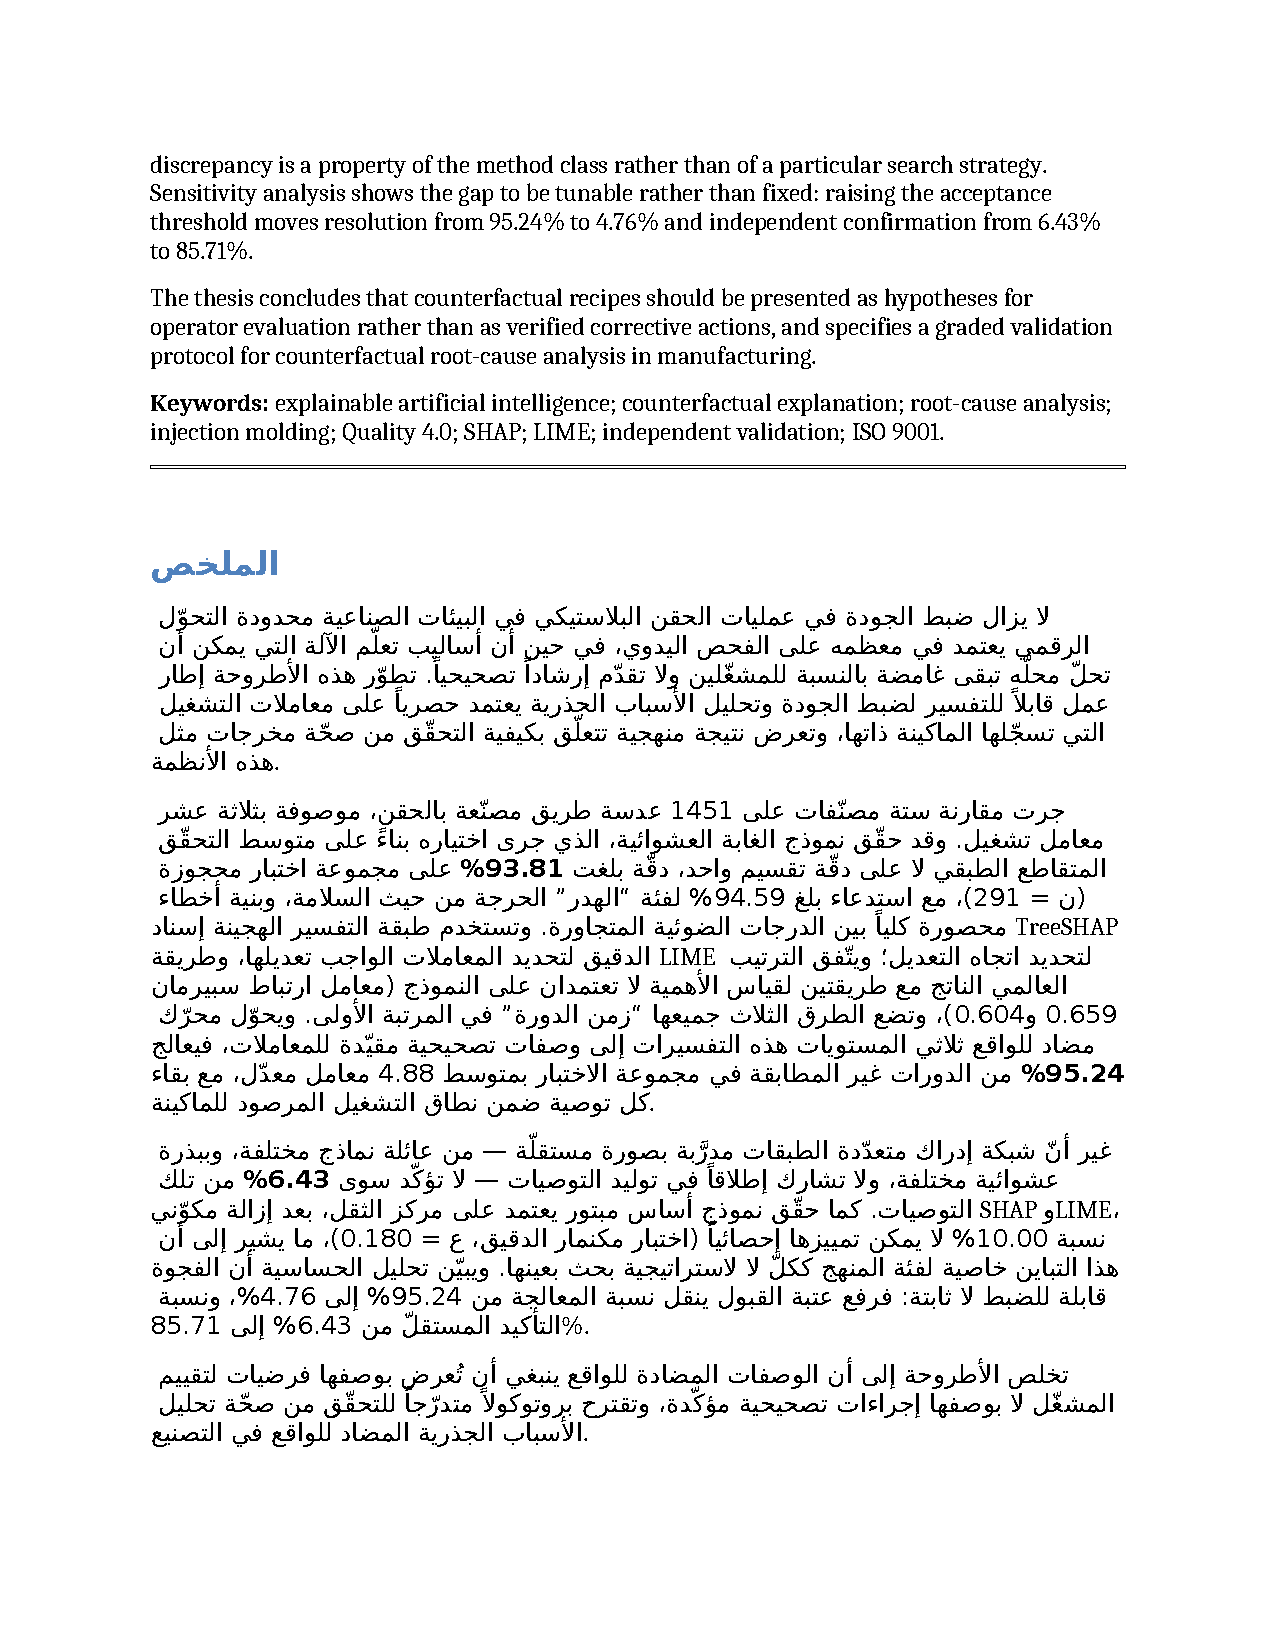
\includepdf[pages=-,pagecommand={
  \thispagestyle{empty}
  \addcontentsline{toc}{chapter}{Arabic Abstract}
}]{frontmatter/abstract_ar.pdf}


\tableofcontents
\listoffigures
\listoftables
\chapter*{List of Abbreviations}
\addcontentsline{toc}{chapter}{List of Abbreviations}

\begin{longtable}{@{}ll@{}}
\toprule
\textbf{Abbreviation} & \textbf{Expansion} \\
\midrule
\endhead
ANOVA & Analysis of Variance \\
CF & Counterfactual \\
CPS & Cyber-Physical System \\
Cp, Cpk & Process Capability Index; Centred Process Capability Index \\
CV & Cross-Validation \\
DT & Decision Tree \\
GB & Gradient Boosting \\
GBT & Gradient-Boosted Trees \\
IIoT & Industrial Internet of Things \\
IMM & Injection Molding Machine \\
ISO & International Organization for Standardization \\
kNN / KNN & k-Nearest Neighbours \\
LIME & Local Interpretable Model-agnostic Explanations \\
LLM & Large Language Model \\
LSL / USL & Lower / Upper Specification Limit \\
ML & Machine Learning \\
MLP & Multilayer Perceptron \\
NN & Nearest Neighbour \\
OEE & Overall Equipment Effectiveness \\
OPC UA & Open Platform Communications Unified Architecture \\
PSI & Population Stability Index \\
RBAC & Role-Based Access Control \\
RCA & Root-Cause Analysis \\
RF & Random Forest \\
ROC & Receiver Operating Characteristic \\
RQ & Research Question \\
SHAP & SHapley Additive exPlanations \\
SME & Small and Medium-sized Enterprise \\
SPC & Statistical Process Control \\
SVM & Support Vector Machine \\
TreeSHAP & Tree-structured SHAP (exact Shapley values for tree ensembles) \\
U\textsubscript{0} & Photometric General Uniformity \\
XAI & Explainable Artificial Intelligence \\
XGB & XGBoost (Extreme Gradient Boosting) \\
ZDM & Zero-Defect Manufacturing \\
\bottomrule
\end{longtable}


% ---------------- MAIN MATTER (arabic numerals) ----------------
\mainmatter
\hypertarget{introduction}{%
\chapter{Introduction}\label{introduction}}

\hypertarget{background-and-motivation}{%
\section{1.1 Background and Motivation}\label{background-and-motivation}}

The plastics sector occupies a substantial position in Palestinian manufacturing, supplying construction, agriculture, packaging, and household-goods markets both domestically and for export. Injection molding is among its most widely used processes, valued for its ability to produce dimensionally complex parts at high volume and low unit cost.

\emph{{[}Insert here the sector's contribution to national output, with a citation to the Palestinian Central Bureau of Statistics or an equivalent published source. The research proposal on which this thesis builds stated a figure of approximately 15\% of GDP for the plastics industry; that figure is uncited and appears inconsistent with published estimates of the size of Palestinian manufacturing as a whole, and should not be reproduced without verification against a primary statistical source. A similarly uncited figure --- injection molding accounting for approximately 30\% of global plastic production --- should likewise be sourced or removed.{]}}

What is not in doubt, and is documented in the sector literature reviewed in §2.2.5, is the character of quality control in these facilities. Inspection is predominantly manual: operators visually check molded parts, and the judgement recorded --- where it is recorded at all --- is a pass or fail entered by hand. This approach carries well-understood limitations. Human inspection performance varies with fatigue, training, and attention; subtle or internal defects are frequently invisible to the eye; and as production volume rises, end-of-line inspection becomes a throughput bottleneck as well as a reliability one.

Behind the inspection problem sits a broader digital-transformation gap. The infrastructure of Industry 4.0 --- sensor data collection, real-time analytics, automated quality feedback --- has made substantial inroads in large manufacturers globally and remains sparse in the small and medium enterprises that constitute most of the Palestinian sector. Limited capital, scarce specialist expertise, and short payback expectations make sensor-rich or vision-based solutions difficult to justify. The consequence is reactive rather than preventive quality management: process data that could anticipate defects is often neither collected nor analysed, even where the machine already produces it.

This last observation is the motivating premise of the thesis. A modern injection molding machine records, for every cycle it runs, a substantial set of process parameters --- temperatures, pressures, forces, screw positions, and timings --- as a matter of ordinary operation. That data exists, costs nothing additional to obtain, and is largely unused. If quality can be predicted, explained, and corrected from those parameters alone, then intelligent quality control becomes available to a factory that cannot afford a camera system or an in-mold sensor.

There is a further pressure that makes this timely. Many Palestinian manufacturers pursue ISO 9001 certification, frequently because customers require it. ISO 9001:2015 specifies what must be monitored, evidenced, and corrected; it does not supply the means. A system that records what was found, why, what correction was advised, and on what basis produces precisely the audit trail the standard requires --- turning a compliance burden into a by-product of ordinary operation.

\hypertarget{the-injection-molding-quality-problem}{%
\section{1.2 The Injection Molding Quality Problem}\label{the-injection-molding-quality-problem}}

Injection molding is a cyclic process in which molten thermoplastic is plasticized in a heated barrel, injected into a mold cavity under pressure, packed to compensate for shrinkage as it solidifies, cooled to rigidity, and ejected. Part quality depends on the precise control of parameters at every stage: melt and mold temperature govern flow and shrinkage, injection pressure and speed determine how completely and uniformly the cavity fills, and packing and cooling times control dimensional stability. When these parameters are well tuned the process produces consistent parts; when they drift, characteristic defects emerge --- short shots, sink marks, warpage, flash, burn marks.

Quality is difficult to control for two reasons that recur throughout this thesis. First, the parameters are strongly coupled and nonlinear in their effect: a change made to correct one defect commonly induces another, which is why the classical practice of adjusting one setting at a time and observing the next few shots is slow and unreliable. Second, the quality-relevant outcome is often not observable at the machine. In the case examined here --- injection-molded road lenses whose quality is defined by photometric general uniformity --- the measurement that defines conformance requires laboratory analysis and cannot be performed in-line at production rate. The parameters that determine quality are recorded continuously; the quality itself is not. A fuller treatment of the process, its defect modes, and the applicable standards is given in §2.2.

\hypertarget{problem-statement}{%
\section{1.3 Problem Statement}\label{problem-statement}}

This thesis addresses two distinct problems. They are stated separately because they are of different kinds, and because the second is what distinguishes the work from a systems-integration exercise.

\hypertarget{problem-1-practical}{%
\subsection{Problem 1 --- Practical}\label{problem-1-practical}}

\textbf{Manual quality control cannot deliver the consistency that formal quality standards require, and the machine learning methods that could replace it are not usable in their current form by the people who would have to rely on them.}

The state of the art in molding quality prediction reaches accuracies above 90\% using tree ensembles and neural networks on process-parameter data. But these models are black boxes: they issue a verdict without a rationale. An operator with limited exposure to AI, presented with an unexplained classification, may reasonably override or ignore it, and a quality manager cannot enter an unexplained verdict into a corrective-action record. More fundamentally, a prediction is not an instruction. A model that reports ``this cycle will produce waste'' leaves entirely open the question the operator actually faces --- \emph{what should I change?} The gap between accurate prediction and actionable guidance is the practical problem, and it is compounded in the target context by the requirement that any solution work on the machine's existing data, without added sensing.

\hypertarget{problem-2-methodological}{%
\subsection{Problem 2 --- Methodological}\label{problem-2-methodological}}

\textbf{Counterfactual explanations in quality control are conventionally validated by the same model that generated them, and this circularity is almost never tested.}

Counterfactual explanation is the natural bridge from prediction to action in a process-control setting: because the model's input features \emph{are} machine settings, the minimal input change that flips the model's decision is directly a corrective work instruction. The method is well developed, with an established set of desiderata --- validity, proximity, sparsity, plausibility, actionability.

The first of those desiderata contains a structural problem. A counterfactual is deemed \emph{valid} if the model classifies it as the desired class. But the counterfactual was produced by searching that same model's decision surface until it did. The criterion by which the recommendation is judged is identical to the objective by which it was constructed, so a search that terminates when the model is satisfied will, by construction, report success. What is measured is the competence of the optimiser, not the correctness of the recommendation.

This would be harmless if trained models faithfully represented the processes they model. The critical literature establishes that they do not, in specific and documented ways: post-hoc explanations can reflect artefacts the model learned rather than knowledge present in the data; counterfactuals can be perfectly valid under a model while occupying regions of feature space where no real production has ever occurred. Yet surveys of evaluation practice find that one XAI paper in three evaluates exclusively on anecdotal evidence, and that only about a fifth of published counterfactual methods have been tested with users at all.

The consequence is that a practitioner deploying counterfactual root-cause analysis in a factory has \textbf{no basis on which to calibrate trust in its output}, because the discrepancy between what such a system reports about itself and what an independent check would confirm has never been measured in an industrial setting. Quantifying that discrepancy --- and determining whether it is a property of one algorithm or of the approach as a class --- is the methodological problem this thesis addresses.

\hypertarget{research-questions}{%
\section{1.4 Research Questions}\label{research-questions}}

Five research questions follow from the two problems above.

\textbf{RQ1.} Can a reproducible multi-class classifier for molded-product quality be established from machine-native process-parameter data alone, without vision systems or added in-mold sensing?

\textbf{RQ2.} Can SHAP and LIME provide operator-interpretable explanations of quality classifications at both global and local scope, and do those explanations agree with importance measures that do not consult the model?

\textbf{RQ3.} Can counterfactual search convert those explanations into actionable, physically bounded parameter recipes that move non-conforming cycles into the conforming region?

\textbf{RQ4.} \emph{(The thesis's own question.)} Do counterfactual recipes validated by the generating classifier survive validation by an independent model --- and if not, is the resulting discrepancy a property of one search algorithm or of the method class?

\textbf{RQ5.} How do the resulting artefacts integrate into a Quality 4.0 framework aligned with ISO 9001 --- process capability monitoring, traceability, drift detection, and operator-facing reporting?

RQ1 to RQ3 are questions about whether a thing can be built, and their expected answers are affirmative; the literature suggests that each component is achievable and the contribution in answering them lies in the integration and in the machine-native constraint. \textbf{RQ4 is different in kind.} It does not ask whether something can be built but whether what has been built can be believed, and its answer is not known in advance. It is flagged here as the thesis's own question because the entire methodology of Chapter 3 --- the independent verifier, the ablated baseline, the sensitivity sweep, the split discipline --- exists to make it answerable, and because its answer is the principal finding reported.

\hypertarget{objectives-and-scope}{%
\section{1.5 Objectives and Scope}\label{objectives-and-scope}}

\hypertarget{original-objectives-and-what-was-delivered}{%
\subsection{1.5.1 Original Objectives and What Was Delivered}\label{original-objectives-and-what-was-delivered}}

The research proposal on which this thesis is based set four objectives. Each is restated below with a plain statement of what was delivered against it.

\textbf{Objective 1 --- Conduct a scoping literature review of AI-driven quality control for injection molding, identifying key gaps and areas for improvement.}
\emph{Delivered, and extended.} Chapter 2 covers the five domains originally scoped and adds a section (§2.7) surveying how explanations and counterfactuals are validated in the literature. That addition was not anticipated in the proposal; it became necessary once the empirical finding emerged, because without it the finding would have had no gap in the literature to occupy.

\textbf{Objective 2 --- Reproduce and validate the findings of the reference study to establish a baseline.}
\emph{Delivered, with an explicit protocol caveat.} Six algorithms were compared and a Random Forest champion established at 93.81\% accuracy on a held-out test split, with an algorithm ranking and per-class profile consistent with the reference. The hyperparameter configuration was adopted from the reference with five documented deviations (§3.4.3). Because this work uses a held-out split while the reference cross-validates over its full dataset, the two accuracy figures are \textbf{not directly comparable}, and no claim of parity or superiority is made anywhere in this thesis.

\textbf{Objective 3 --- Enhance the validated model by integrating XAI and RCA layers.}
\emph{Delivered, and it is the substantive body of the work.} A hybrid SHAP-plus-LIME explanation layer (§3.5) and a three-tier counterfactual RCA engine with an independent verifier (§3.6) were built, deployed as a working application, and evaluated across the full held-out population.

\textbf{Objective 4 --- Acquire a new dataset, or generate an augmented one, to test the enhanced model against a second data source.}
\textbf{\emph{Not pursued.}} No new dataset was acquired and no data augmentation was performed. The work instead deepened the evaluation on the reference dataset in three directions the proposal did not anticipate: a held-out test split reserved from every selection decision, a centroid-ablation baseline permitting a controlled comparison of search strategies, and a two-dimensional sensitivity sweep characterising the engine's operating envelope. This is a genuine deviation from the proposal, and in the author's assessment the substitution strengthened the work --- the ablation study is what allows the central finding to be generalised beyond a single algorithm --- but it is a deviation, and it is stated here rather than left for a reader holding the proposal to discover.

\hypertarget{correcting-the-record-on-accuracy}{%
\subsection{1.5.2 Correcting the Record on Accuracy}\label{correcting-the-record-on-accuracy}}

The proposal anticipated that the enhanced model would achieve accuracy superior to the reference baseline. \textbf{That was not achieved, and it is not the contribution of this thesis.}

Under a protocol that is not directly comparable, this work reports 93.81\% on a held-out test split against the reference's 95.04\% mean accuracy from five-fold cross-validation over its full dataset. The two figures differ in denominator, in training-set size, and in averaging procedure, and the difference between them carries no interpretable meaning (§4.2.5). What the comparison supports is the weaker and sufficient claim that the reimplementation behaves like the model it reimplements --- which is what licenses using it as the substrate for the counterfactual work.

The contribution of this thesis lies elsewhere: in the explanation and root-cause layers built on top of that model, and above all in the finding about how the output of such layers should be validated. Accuracy improvement was never the mechanism by which this work was going to be useful, and stating that plainly here prevents the thesis being read against a benchmark it does not claim to meet.

\hypertarget{scope}{%
\subsection{1.5.3 Scope}\label{scope}}

\textbf{In scope.} Quality classification, explanation, and counterfactual root-cause analysis from the thirteen machine-native process parameters of a single published dataset; independent verification of counterfactual output; ablation comparison and sensitivity analysis; and the supporting Quality 4.0 modules --- process capability, traceability, drift monitoring, OEE simulation, LLM reporting, operator notification, and role separation --- as infrastructure demonstrating deployment feasibility.

\textbf{Out of scope, and why.}

\emph{Physical validation.} No counterfactual recipe generated in this work was executed on an injection molding machine. This requires access to an instrumented machine producing the same part, production time, photometric measurement capability, and tolerance for producing scrap during a trial, none of which were available. It is the principal limitation of the work (§5.4) and the principal item of future work (§6.4).

\emph{Vision-based inspection.} Excluded by the machine-native design constraint, which is the premise of the deployment argument rather than an omission.

\emph{Process optimisation and closed-loop control.} The system recommends; it does not write setpoints back to the machine. Two modules present in early development --- a genetic process optimiser and a REST API server --- were removed as out of scope, on the grounds that they broadened the artefact without contributing to the research questions.

\emph{Multi-product and multi-machine generalisation.} All results derive from one product, one machine, and one manufacturer.

\hypertarget{contributions}{%
\section{1.6 Contributions}\label{contributions}}

The contributions are listed in order of strength. Each is stated at the level the evidence supports; §6.3 restates them alongside what is explicitly not claimed.

\textbf{Contribution 1 --- An independently-validated counterfactual RCA architecture that exposes and quantifies the circularity gap.} On a held-out test split of real injection-molding cycles, the engine reports a resolution rate of \textbf{95.24\%} while an independently trained verifier --- of a different model family, a different seed, and taking no part in the counterfactual search --- confirms \textbf{6.43\%} of those resolutions. To the author's knowledge this is the first quantification of that discrepancy on a real industrial process dataset, measured across a complete evaluation population rather than on selected illustrative cases.

\textbf{Contribution 2 --- Evidence that the gap is not attributable to search strategy.} A centroid-ablation baseline, which removes SHAP feature selection and LIME directional guidance while holding the acceptance criterion, champion model, verifier, step size and iteration budget constant, achieves a statistically indistinguishable confirmation rate (10.00\% against 6.43\%; McNemar exact test, \emph{p} = 0.180 on the test split). Combined with the structural similarity of the two methods, this is evidence that the confirmation rate is a property of the shared approach rather than of either implementation --- which is what generalises Contribution 1 beyond the particular engine built here.

\textbf{Contribution 3 --- Characterisation of the gap as a tunable operating envelope.} Two sensitivity sweeps across ten configurations and two data splits show the resolution-versus-confirmation trade-off to be continuous and near-monotonic in the acceptance threshold (95.24\% → 4.76\% resolution against 6.43\% → 85.71\% confirmation), and --- less expectedly --- inversely related to search effort, with a reduced iteration budget doubling independent confirmation. This reframes a single unfavourable figure as a design parameter with a measurable cost curve.

\textbf{Contribution 4 --- A hybrid SHAP-plus-LIME explanation layer for multi-class injection-molding quality.} SHAP selects which parameters to adjust; LIME determines the direction. The division uses each method for the quantity it estimates most reliably, yields deterministic feature selection through exact TreeSHAP, and produces attributions that two model-free importance methods independently corroborate (Spearman r = 0.659 and 0.604), with all three ranking the same parameter first.

\textbf{Contribution 5 --- An integrated Quality 4.0 framework deployed as a working application, with a fully reproducible evaluation pipeline.} An eight-page application combining ISO 9001 process-capability monitoring, SQLite traceability, PSI and Page-Hinkley drift detection, OEE simulation, LLM-generated shift reporting, and operator notification, operating on commodity CPU hardware in approximately half a second per cycle. The evaluation is reproducible end to end from raw data by two orchestration scripts, with documented hyperparameter provenance including five deviations from the reference configuration and an empirical resolution of the tree-depth ambiguity.

\hypertarget{thesis-organization}{%
\section{1.7 Thesis Organization}\label{thesis-organization}}

\textbf{Chapter 2} reviews the literature across five domains: the injection molding process and its quality challenges, machine learning for quality prediction, explainable AI including a detailed treatment of counterfactual explanation and its desiderata, root-cause analysis in smart manufacturing, and Quality 4.0. Its pivotal section (§2.7) surveys how explanations are actually validated in practice and establishes that validation against the generating model is the norm --- the gap that motivates RQ4.

\textbf{Chapter 3} specifies the methodology and system design under a design-science frame: the dataset and its conformance definition, the preprocessing pipeline and split discipline, model selection with full hyperparameter provenance, the explanation layer, the three-tier counterfactual engine with its independent verifier and ablated baseline, the supporting Quality 4.0 modules, the implementation, and the evaluation design.

\textbf{Chapter 4} reports results: classification performance with priority on \emph{Waste} recall, explanation-layer results including agreement with model-free importance methods, counterfactual resolution rates with a worked case, the independent validation finding and its ablation comparison with statistical testing, the tier-cascade sensitivity sweeps, drift-detector validation, and the expert evaluation sub-study.

\textbf{Chapter 5} discusses what the results mean: the physical interpretation of the attributions, why self-validated counterfactuals overstate resolution and why the ablation generalises that finding, what a defensible validation protocol would require, the practical requirements for deployment in the target context, and a full statement of limitations and threats to validity.

\textbf{Chapter 6} answers each research question directly, restates the contributions with their explicit boundaries, and sets out future work --- foremost the physical validation trial that would convert the central finding from a statement about two models into a statement about a process.

\textbf{Appendices} provide the full parameter specification, the hyperparameter provenance document, the expert evaluation instrument, the artefact index mapping every reported figure to its source file, selected code listings, application screenshots, and the declaration of AI tool use required under university policy.

\hypertarget{literature-review}{%
\chapter{Literature Review}\label{literature-review}}

\hypertarget{review-approach}{%
\section{2.1 Review Approach}\label{review-approach}}

\hypertarget{rationale-for-a-scoping-review}{%
\subsection{2.1.1 Rationale for a Scoping Review}\label{rationale-for-a-scoping-review}}

This chapter situates the present research within the existing body of knowledge spanning five intersecting domains: machine learning (ML) for injection molding quality prediction, explainable artificial intelligence (XAI), counterfactual explanation, root-cause analysis (RCA), and the emerging paradigm of Quality 4.0. A scoping review approach is adopted rather than a full systematic review. Arksey and O'Malley {[}1{]} characterise scoping studies as appropriate where the aim is to map the key concepts underpinning a research area and the main sources of evidence available, particularly where the area is complex or has not previously been reviewed comprehensively. Both conditions hold here. The research problem is inherently multidisciplinary, and the specific intersection it occupies --- interpretable, machine-native, counterfactual root-cause analysis with independent verification --- has no dedicated review literature of its own. Rather than examining a single technique in isolation, this review maps the state of each contributing domain, evaluates representative studies critically, and isolates the specific gaps that the proposed framework addresses.

An important consequence of this choice should be stated at the outset. A scoping review favours breadth of coverage over exhaustive enumeration and does not attempt formal quality appraisal of every included study. The claims of absence made in this chapter --- most importantly, the claim in Section 2.7 that independent validation of counterfactual explanations is rare --- are therefore claims about what a structured search of the major databases surfaces, not proofs of non-existence. They are stated in those terms throughout.

\hypertarget{search-protocol}{%
\subsection{2.1.2 Search Protocol}\label{search-protocol}}

The literature was gathered through structured searches of four academic databases --- IEEE Xplore, ScienceDirect, SpringerLink, and MDPI --- supplemented by the ACM Digital Library for the explainability and counterfactual literature, by forward and backward citation tracing from key papers, and by targeted searches of Google Scholar for grey literature relevant to the Palestinian industrial context.

Search strings combined terms across the contributing domains. Representative strings included: (``injection molding'' OR ``injection moulding'') AND (``machine learning'' OR ``quality prediction''); (``explainable AI'' OR XAI OR SHAP OR LIME) AND (manufacturing OR ``quality control''); (``counterfactual explanation'' OR ``algorithmic recourse'') AND (evaluation OR validation OR plausibility); (``root cause analysis'') AND (``machine learning'' OR ``zero-defect manufacturing''); and (``Quality 4.0'') AND (``Industry 4.0'' OR ``ISO 9001'').

Studies were included if they applied data-driven or interpretable methods to manufacturing quality control, with priority given to injection molding, and if published primarily between 2015 and 2025. Seminal earlier works were retained where they remain foundational --- Ribeiro's support-vector work on molding quality monitoring and the in-process measurement studies of Gao and Gordon are examples. Studies were excluded if they addressed unrelated manufacturing processes without transferable methodology, or if they reported insufficient methodological detail for the claims made to be assessed. For the counterfactual and explanation-evaluation literature the domain restriction was deliberately relaxed, because the methodological problem examined in Section 2.7 is not specific to manufacturing and the relevant work is concentrated in the general machine-learning venues.

Screening counts are not reported. The search was iterative and interleaved with the design of the artefact rather than executed as a single frozen protocol, so a PRISMA-style flow diagram would impose a false retrospective precision on the process. The protocol is therefore described in prose, and the review is presented as a scoping map rather than an auditable systematic review.

\hypertarget{structure-of-the-chapter}{%
\subsection{2.1.3 Structure of the Chapter}\label{structure-of-the-chapter}}

The chapter builds a cumulative argument. Section 2.2 establishes the injection molding process, the parameters that govern part quality, the defect modes that arise when those parameters drift, and the industrial reality of Palestinian and comparable manufacturers. Section 2.3 surveys machine learning for quality prediction, examines in detail the benchmark study on which this thesis builds, and argues that the field's evaluation practice stops at predictive accuracy. Section 2.4 covers XAI foundations, develops the counterfactual explanation literature and its desiderata in depth, and shows that explainability remains almost absent from injection molding practice. Section 2.5 reviews RCA from classical tools to data-driven methods and positions counterfactual reasoning as a route to actionable diagnosis. Section 2.6 frames the discussion within Quality 4.0, statistical process capability, and concept drift. Section 2.7 --- the pivot of the chapter --- surveys how explanations and counterfactuals are actually validated in the literature and establishes that validation against the generating model is the norm and independent validation the exception. Section 2.8 consolidates the gaps and states how each is addressed.

\begin{center}\rule{0.5\linewidth}{0.5pt}\end{center}

\hypertarget{injection-molding-and-quality-challenges}{%
\section{2.2 Injection Molding and Quality Challenges}\label{injection-molding-and-quality-challenges}}

\hypertarget{process-fundamentals}{%
\subsection{2.2.1 Process Fundamentals}\label{process-fundamentals}}

Injection molding is a cyclic manufacturing process in which molten thermoplastic is shaped into solid parts through five sequential stages: plasticizing, injection, packing, cooling, and ejection. During plasticizing, pellets are melted in a heated barrel by a rotating screw. During injection, the screw advances to force the melt into the mold cavity under high pressure. The packing phase then maintains pressure to compensate for volumetric shrinkage as the material begins to solidify. The cooling phase allows the part to gain sufficient rigidity for handling, and finally the mold opens for ejection before the next cycle begins. Cycle times range from seconds to minutes depending on part geometry, wall thickness, and material, which makes the process highly efficient for mass production of dimensionally consistent parts {[}2{]}, {[}3{]}.

The process is best understood as a sequence of energy and material transfers, each of which is instrumented on a modern machine. The screw's rotation and back pressure govern melting; its forward velocity and the resulting hydraulic or specific injection pressure govern cavity filling; the clamping unit resists the separating force generated inside the cavity; and the thermal circuits of barrel and mold govern solidification. Every one of these quantities is measured by the machine's own control system as a matter of ordinary operation, a fact that becomes central to the argument of this thesis.

\hypertarget{process-parameters-and-their-effect-on-part-quality}{%
\subsection{2.2.2 Process Parameters and Their Effect on Part Quality}\label{process-parameters-and-their-effect-on-part-quality}}

Part quality depends critically on the precise control of process parameters at each stage. Melt and mold temperature govern flow behaviour, crystallinity, and shrinkage. Injection pressure and speed determine how completely and how uniformly the cavity fills, and how much molecular orientation is frozen into the part. Packing (hold) pressure and hold time determine how much additional material is fed into the cavity to compensate for contraction. Cooling time and mold temperature determine dimensional stability and residual stress at ejection. Zhao et al.~{[}4{]}, in a review of sensing, optimization, and control for intelligent injection molding, characterise these relationships as strongly nonlinear and mutually coupled: a change made to correct one defect commonly induces another, which is precisely why single-parameter trial-and-error adjustment is slow and unreliable in practice.

Two properties of this parameter--quality mapping matter for the present work. First, it is direct: the parameters are not proxies for quality-relevant physics, they \emph{are} the quality-relevant physics, which is what makes machine-native data a legitimate basis for quality prediction rather than a compromise. Second, it is coupled: because parameters interact, a corrective recommendation that adjusts several parameters simultaneously is not merely a convenience but a requirement, and the correctness of such a multi-parameter recommendation cannot be established by inspecting each parameter in isolation. This second property anticipates the validation problem developed in Section 2.7.

\hypertarget{common-defect-modes}{%
\subsection{2.2.3 Common Defect Modes}\label{common-defect-modes}}

Even within a controlled process, injection-molded parts exhibit recurring defects whose causes span material, machine, and environmental factors. Table 2.1 summarises the most common defects and their principal causes, synthesised from established process and mold-design references {[}2{]}, {[}3{]}, {[}4{]}.

\textbf{Table 2.1.} Common injection molding defects and their principal causes.

\begin{longtable}[]{@{}
  >{\raggedright\arraybackslash}p{(\columnwidth - 4\tabcolsep) * \real{0.3333}}
  >{\raggedright\arraybackslash}p{(\columnwidth - 4\tabcolsep) * \real{0.3333}}
  >{\raggedright\arraybackslash}p{(\columnwidth - 4\tabcolsep) * \real{0.3333}}@{}}
\toprule\noalign{}
\begin{minipage}[b]{\linewidth}\raggedright
Defect
\end{minipage} & \begin{minipage}[b]{\linewidth}\raggedright
Description
\end{minipage} & \begin{minipage}[b]{\linewidth}\raggedright
Principal causes
\end{minipage} \\
\midrule\noalign{}
\endhead
\bottomrule\noalign{}
\endlastfoot
Shrinkage & Dimensional reduction as the part cools & Inherent material contraction; insufficient packing pressure or hold time \\
Warpage & Distortion or twisting of the part & Differential or uneven cooling; non-uniform wall thickness; anisotropic shrinkage \\
Short shot & Incompletely filled cavity & Insufficient injection pressure or speed; inadequate material feed; restricted gates or venting \\
Burn marks & Charred dark spots near end of fill & Trapped air or gas combusting under compression; excessive injection speed or melt temperature; poor venting \\
Flash & Thin excess plastic at parting lines & Insufficient clamping force; over-packing; mold wear or misalignment \\
Sink marks & Surface depressions over thick sections & Localized shrinkage; inadequate packing pressure or cooling time; non-uniform wall thickness \\
Weld lines & Visible seams where flow fronts meet & Low melt or mold temperature; slow injection; unfavourable gate placement \\
\end{longtable}

These causes fall into three broad groups: material-related (resin grade, moisture content, contamination, regrind fraction), machine- or process-related (incorrect temperatures, pressures, speeds, or timings, and equipment faults such as worn check rings or degraded heater bands), and environment- or operator-related (ambient humidity, cooling-water temperature variability, and inconsistent manual operation).

Critically for this thesis, the machine- and process-related group is precisely the group captured directly by an injection molding machine's own sensors. A substantial fraction of defect causes is therefore, in principle, diagnosable from machine-native data alone, without recourse to vision systems or laboratory measurement. The corollary is equally important and is stated here so that Chapter 5 can return to it: causes in the material and environmental groups are \emph{not} represented in machine-parameter data, and no method operating on that data alone can be expected to diagnose them. A residue of cases that resist parameter-based correction is therefore anticipated by the physics of the process, not merely by the limitations of any particular algorithm.

\hypertarget{quality-standards-for-the-reference-product}{%
\subsection{2.2.4 Quality Standards for the Reference Product}\label{quality-standards-for-the-reference-product}}

The dataset used in this thesis concerns injection-molded road lenses produced by iGuzzini Illuminazione, and its quality labels derive from a photometric standard rather than from visual defect inspection. Polenta et al.~{[}5{]} label each lens by measuring its general uniformity, U\textsubscript{0}, under laboratory photometric analysis, and define four classes with reference to the requirement in UNI EN 13201-2:2016 {[}6{]} that M1-class lenses for motorised roads achieve U\textsubscript{0} greater than 0.4:

\begin{itemize}
\tightlist
\item
  \textbf{Waste} (U\textsubscript{0} \textless{} 0.4): non-compliant with the standard and to be discarded. Original label 1.
\item
  \textbf{Acceptable} (0.4 ≤ U\textsubscript{0} \textless{} 0.45): compliant with the standard and accepted by the manufacturer, though below the internal production target. Original label 2.
\item
  \textbf{Target} (0.45 ≤ U\textsubscript{0} ≤ 0.5): considered optimal by the manufacturer. Original label 3.
\item
  \textbf{Inefficient} (U\textsubscript{0} \textgreater{} 0.5): compliant with the standard, but achieved at an unnecessary expenditure of machine resources, and therefore to be avoided. Original label 4.
\end{itemize}

This labelling scheme has two features that shape the whole thesis and must be understood before the results of Chapter 4 can be read correctly. First, the classes are ordinal in photometric terms but not monotonic in desirability: \emph{Inefficient} denotes over-performance, not a defect. A part labelled \emph{Inefficient} is saleable; it is simply uneconomic to produce. Second, and following from the first, the operationally meaningful binary distinction is not ``compliant versus non-compliant'' but ``at the production target versus not at it.'' Chapter 3 accordingly defines the conforming set as \{Acceptable, Target\}, and that definition follows directly from the standard and the manufacturer's stated economics rather than from any modelling convenience.

The reliance on a laboratory photometric measurement also explains why the quality label is expensive to obtain and why predicting it from process data has industrial value: the measurement that defines quality here cannot be performed in-line at production rate.

\hypertarget{industrial-reality-in-palestine-and-comparable-ecosystems}{%
\subsection{2.2.5 Industrial Reality in Palestine and Comparable Ecosystems}\label{industrial-reality-in-palestine-and-comparable-ecosystems}}

The quality challenges above take on a particular character in developing industrial ecosystems. A study of the Palestinian plastics sector reports that most manufacturers continue to rely on traditional processes with limited investment in modern automation, prioritising immediate cost reduction over digital adoption {[}7{]}. In such settings, quality inspection is typically manual: operators visually check parts, an approach limited by fatigue, inconsistent training, and low throughput, and one that cannot detect internal or parametric deviations at all. As production volumes grow, manual inspection becomes a throughput bottleneck as well as a reliability one.

Beyond inspection, these enterprises face a broader digital transformation gap. Full integration of digital monitoring --- from machine sensors through to automated quality feedback --- is rare in smaller firms. Limited capital, scarce specialist expertise, and infrastructure constraints make high-end solutions difficult to justify against short payback expectations. The result is reactive rather than preventive quality management: process data that could predict defects is often neither collected nor analysed, even where the machine already produces it.

Many such firms nonetheless pursue ISO 9001 certification as a foundation for systematic quality control, frequently because customers require it. ISO 9001:2015 {[}8{]} establishes the management framework --- defined processes, monitoring, traceability of nonconforming output, documented corrective action, and continual improvement --- while Quality 4.0 supplies modern means of achieving these ends through data and analytics. The two are complementary rather than competing: the standard specifies what must be controlled and evidenced, and data-driven methods determine how that control can be exercised with greater insight. This complementarity matters for the present work, because an interpretable, low-cost quality system that runs on existing machine data offers a pragmatic entry point to Quality 4.0 for firms that cannot afford sensor-rich or vision-based infrastructure.

A caveat is warranted. The empirical basis for characterising the Palestinian sector is thin --- a small number of studies, none recent --- and this thesis does not itself collect field data on local factories. The Palestinian context is therefore treated throughout as a motivating deployment scenario that constrains the design (no added sensors, low compute, operator-facing output), not as an empirically characterised setting about which the thesis makes findings.

\begin{center}\rule{0.5\linewidth}{0.5pt}\end{center}

\hypertarget{machine-learning-for-quality-prediction-in-injection-molding}{%
\section{2.3 Machine Learning for Quality Prediction in Injection Molding}\label{machine-learning-for-quality-prediction-in-injection-molding}}

\hypertarget{classification-approaches-and-reported-performance}{%
\subsection{2.3.1 Classification Approaches and Reported Performance}\label{classification-approaches-and-reported-performance}}

Before deep learning became prevalent, classical models --- support vector machines (SVM), k-nearest neighbours (kNN), decision trees, and ensemble methods --- dominated injection molding quality prediction, valued for their tractability on small tabular datasets and their computational efficiency. Ribeiro {[}9{]} trained SVM classifiers on process features to detect fault conditions in a plastic injection molding process, reporting high accuracies and outperforming a contemporary neural network. The result is frequently cited as evidence of SVM viability, but it should be read with caution: the study used a single machine and a modest, defect-specific dataset, so its figures establish feasibility rather than transferability to the multi-machine, imbalanced conditions typical of SME production.

Subsequent work has broadened both the algorithm set and the data basis. Párizs et al.~{[}10{]} compared several classifiers for quality prediction in a multi-cavity mold using pressure-derived features, finding tree-based ensembles and random forest superior and kNN weakest. Ogorodnyk et al.~{[}11{]} applied classification methods to thermoplastic molding parameters and reached comparable conclusions. Silva et al.~{[}12{]} report an industrial deployment in a Portuguese molding company, covering the full path from data collection through data augmentation and human-in-the-loop labelling to real-time classification and operator alerting --- a useful counterpoint to purely offline studies, and one of the few papers to treat labelling cost as a first-class engineering problem.

The consistent finding across these studies is that ensembles outperform single learners while retaining tractable feature-importance information. This justifies the selection of a tree ensemble as the predictive core of an interpretable framework. Classical models thus offer a favourable balance of accuracy, speed, and transparency --- but, as Section 2.3.4 argues, the literature evaluates them almost exclusively on predictive accuracy, leaving their explanatory potential largely unexploited.

\hypertarget{the-polenta-et-al.-2022-benchmark}{%
\subsection{2.3.2 The Polenta et al.~(2022) Benchmark}\label{the-polenta-et-al.-2022-benchmark}}

One study warrants detailed treatment because it supplies both the dataset and the performance baseline for this thesis. Polenta et al.~{[}5{]} compared six classifiers --- kNN, decision tree, random forest, gradient-boosted trees (GBT), SVM, and a multilayer perceptron (MLP) --- on 1,451 injection-molded road lenses produced by iGuzzini Illuminazione on an Engel E-MAC 310/100 machine, described by 13 process parameters and labelled into the four photometric quality classes set out in Section 2.2.4.

\textbf{Dataset.} The 13 parameters are melt temperature, mold temperature, filling time, plasticizing time, cycle time, closing force, clamping force peak value, torque peak value, torque mean value, specific back pressure peak value, specific injection pressure peak value, screw position at the end of hold pressure, and shot volume. Class distribution is relatively balanced: 370 \emph{Waste}, 406 \emph{Acceptable}, 310 \emph{Target}, and 360 \emph{Inefficient}.

\textbf{Protocol.} Hyperparameters were selected by grid search, and results were obtained under stratified five-fold cross-validation over the full dataset, with per-class precision and recall computed by summing the predictions across the five test folds. This protocol detail matters for any comparison drawn against the study: it aggregates over the whole dataset rather than reporting a single held-out test split, so figures from the two protocols are not strictly commensurable. Chapter 4 states this caveat wherever the comparison is made.

\textbf{Results.} Random forest was the strongest model, reaching a macro-averaged F1 of 94.95\% (±1.23\%), followed by GBT at 94.16\% (±0.98\%). Per-class, random forest achieved the highest precision on the critical \emph{Waste} class at 97.22\%, with 94.59\% recall. The authors emphasise that misclassifications between \emph{Waste} and \emph{Acceptable} are the consequential errors, since these correspond to shipping a non-compliant lens or scrapping a compliant one, whereas confusions among \emph{Acceptable}, \emph{Target}, and \emph{Inefficient} all occur within the compliant region.

\textbf{Significance and limitation.} The study's principal strength, and the reason it is adopted as the baseline here, is reproducibility: both the dataset and the comparison source code were publicly released, making it one of very few fully reproducible benchmarks in this domain. Its principal limitation is that it stops at prediction. It ranks classifiers and reports which features the models find relevant, but it does not translate a prediction into a corrective action, and it makes no attempt to explain individual predictions. The gap between ``this lens will be waste'' and ``reduce melt temperature by 6 °C and increase plasticizing time by 0.2 s'' is exactly the gap this thesis sets out to close.

\hypertarget{deep-learning-and-multi-sensor-approaches}{%
\subsection{2.3.3 Deep Learning and Multi-Sensor Approaches}\label{deep-learning-and-multi-sensor-approaches}}

With richer datasets, researchers have turned to deep learning, particularly convolutional neural networks (CNNs) for image-based defect detection. Hu et al.~{[}13{]} adapted a simplified VGG16 network for molding fault diagnosis, reporting 96.67\% accuracy against a weaker baseline network. The reported gain was achieved only after substantial architectural simplification to combat overfitting on a small dataset, illustrating a recurring tension: deep models demand either large data volumes or careful, expertise-intensive tuning, neither of which is readily available in under-digitized facilities.

A distinct strand treats the molding machine as a cyber-physical system and fuses multivariate sensor streams for real-time prediction. Gao et al.~{[}14{]} and Gordon et al.~{[}15{]} embedded a multivariate sensor in the mold cavity to measure melt pressure, temperature, flow-front velocity, and inferred viscosity simultaneously, reporting strong correlations between these in-process signals and final part quality. Their central finding --- that the closer a sensor sits to the polymer, the more predictive its signal becomes --- explains why combined orthogonal in-cavity signals outperform any single machine-level channel. Wang et al.~{[}16{]} pursue the same logic for micro-injection products, characterising quality through cavity-pressure features. Kumar et al.~{[}17{]} combine time-series process profiles with statistical classifiers for closed-loop control, and Tercan et al.~{[}18{]} address a different practical obstacle, applying continual learning with memory-aware synapses so that a warpage-prediction network need not be retrained from scratch when the product changes.

These approaches are powerful, but they share a precondition: they assume the availability of in-mold or retrofit sensors and the infrastructure to stream and store their output at cycle rate. That assumption is exactly the barrier that under-digitized SMEs cannot clear. It reframes the question this thesis addresses --- whether comparable diagnostic value can be extracted from the machine's existing native parameters alone, with no additional sensing. Tercan et al.~{[}18{]} also expose a second brittleness: a purely predictive model tied to one product geometry must be replaced or adapted when the product changes, and offers no interpretable account of \emph{why} its prediction shifted.

\hypertarget{limitations-of-accuracy-only-evaluation}{%
\subsection{2.3.4 Limitations of Accuracy-Only Evaluation}\label{limitations-of-accuracy-only-evaluation}}

Read together, the studies above share an evaluation posture that this thesis treats as a limitation rather than a neutral convention. Performance is reported as accuracy, F1, precision, and recall; models are ranked on those numbers; and the paper ends. Three consequences follow.

First, a model that is accurate is not thereby useful. In a molding plant, a correct prediction that a lens will be \emph{Waste} has value only if it arrives with enough time and enough information to prevent the next lens from also being \emph{Waste}. Accuracy quantifies the first half of that requirement and is silent on the second.

Second, accuracy-only evaluation cannot distinguish models that have learned process physics from models that have learned dataset artefacts. Two classifiers with identical F1 may rest on entirely different feature dependencies, and nothing in the reported metrics discriminates between them. This becomes acute the moment a model is used for anything beyond classification --- most obviously, for generating corrective recommendations, which are only as trustworthy as the dependencies they exploit.

Third, and most consequentially for this thesis, the evaluation vocabulary of the field contains no term for the correctness of a prescription. There is a well-established answer to ``was the classification right?'' and, as Section 2.7 shows, a much weaker one to ``was the recommended correction right?'' The field's metrics were designed for the first question and have been carried over, largely unexamined, to work that is implicitly asking the second.

\hypertarget{vision-based-inspection-versus-machine-parameter-prediction}{%
\subsection{2.3.5 Vision-Based Inspection versus Machine-Parameter Prediction}\label{vision-based-inspection-versus-machine-parameter-prediction}}

A final contrast completes the picture. In advanced factories, vision-based inspection has become the standard for molding quality control, capturing part images and classifying defects with CNNs or feature-based pipelines. Reported performance is high: Asadi et al.~{[}19{]} achieved an F-score of 96.7\% with a local-binary-pattern and SVM pipeline; Muresan et al.~{[}20{]} reported 94\% to 99\% accuracy for bushing-placement classification in automotive components; Zhang et al.~{[}21{]} report further gains using multiplicative feature fusion and attention mechanisms for molded-part defect detection; and the broader review by Chen et al.~{[}22{]} documents the maturity of surface-defect detection across industrial products generally.

For smaller manufacturers, however, vision systems carry practical barriers. Industrial cameras, controlled lighting, and inference hardware represent a capital cost that must be justified per production cell. Reliable imaging demands careful control of illumination and part positioning, since ambient light, variable presentation angle, and surface reflections induce false detections --- a particularly severe constraint for transparent optical parts such as road lenses. And deployment requires integration expertise that most small molders lack {[}7{]}.

There is also a deeper limitation that cost alone does not capture. Vision inspects the \emph{outcome}. It can report that a part is defective with high reliability, but the image contains no information about which machine setting produced the defect; recovering the cause from the symptom requires a separate inferential step that vision data cannot supply. Machine-parameter data has the inverse profile: it is a weaker signal about the outcome, but it is a direct record of the causes. This asymmetry, rather than cost alone, is the substantive argument for machine-native quality control in a root-cause setting.

\begin{center}\rule{0.5\linewidth}{0.5pt}\end{center}

\hypertarget{explainable-artificial-intelligence}{%
\section{2.4 Explainable Artificial Intelligence}\label{explainable-artificial-intelligence}}

Having established that the most accurate quality models are also the least transparent, and that the field's evaluation vocabulary stops short of assessing prescriptions, this section examines the techniques developed to interpret model behaviour and their application to manufacturing.

\hypertarget{taxonomy-of-explanation-methods}{%
\subsection{2.4.1 Taxonomy of Explanation Methods}\label{taxonomy-of-explanation-methods}}

XAI methods are conventionally organised along three axes {[}23{]}.

The first is \textbf{intrinsic versus post-hoc}. Intrinsic models such as decision trees, linear regression, and rule lists expose their logic by construction. Post-hoc methods explain an already-trained model without altering it. Rudin {[}24{]} argues forcefully that for high-stakes decisions the intrinsic route should be preferred, on the grounds that a post-hoc explanation is by definition an approximation of the model and may therefore be wrong in ways that are undetectable to the user. That argument is directly relevant here and is revisited in Section 2.7: this thesis uses post-hoc methods, and Rudin's critique is a substantial part of the reason the work treats independent verification as necessary rather than optional.

The second axis is \textbf{model-agnostic versus model-specific}. Agnostic methods such as LIME, and the general (KernelSHAP) form of SHAP, treat the model as a queryable black-box function and can therefore be applied to anything. Model-specific methods such as TreeSHAP exploit internal structure to compute exact attributions efficiently for tree ensembles.

The third axis is \textbf{global versus local scope}. Global explanations characterise overall model behaviour --- which parameters matter across the whole process --- whereas local explanations justify a single prediction. Root-cause analysis is inherently a local task: the question is never ``what causes waste in general'' but ``what caused \emph{this} cycle to produce waste.''

\hypertarget{shap-and-treeshap}{%
\subsection{2.4.2 SHAP and TreeSHAP}\label{shap-and-treeshap}}

SHAP (SHapley Additive exPlanations) attributes a prediction to its input features using Shapley values from cooperative game theory {[}25{]}. A SHAP value expresses how much a feature moves a prediction above or below the model's expected output, in the model's own output space, and the attributions satisfy local accuracy, missingness, and consistency. Lundberg et al.~{[}26{]} subsequently introduced TreeSHAP, which computes exact Shapley values for tree ensembles in polynomial rather than exponential time, making the method practical for random forests of realistic size and removing the sampling variance that afflicts model-agnostic approximation.

Two properties of SHAP are important for what follows. It is \emph{additive and signed}, so attributions can be aggregated across samples to yield a stable global ranking. But it is \emph{not a statement about intervention}: a SHAP value quantifies a feature's contribution to a prediction given the model and the background distribution, and it does not assert that changing the feature by a given amount will change the outcome by a corresponding amount. Treating SHAP magnitudes as adjustment magnitudes is a category error, and one that the design in Chapter 3 explicitly avoids by using SHAP for feature \emph{selection} only.

\hypertarget{lime-and-local-surrogate-models}{%
\subsection{2.4.3 LIME and Local Surrogate Models}\label{lime-and-local-surrogate-models}}

LIME (Local Interpretable Model-agnostic Explanations) {[}27{]} takes a different route. It perturbs the instance being explained, queries the model on the perturbed samples, weights them by proximity to the original, and fits a sparse linear surrogate to that weighted neighbourhood. The surrogate's coefficients indicate the local direction and strength of each feature's influence.

The distinction from SHAP matters directly for root-cause work. SHAP excels at stable, theoretically grounded feature ranking, but its values are not physical adjustment directions. LIME's local slope, by contrast, maps naturally onto the notion of moving a parameter: a negative coefficient on melt temperature in the neighbourhood of a defective cycle is a statement, however local and however approximate, that reducing melt temperature moves the prediction toward the desired class. This complementarity --- SHAP for \emph{which} parameters, LIME for \emph{which way} --- is exploited directly in the proposed framework. Its weakness is equally relevant: LIME's surrogate is fitted on synthetic perturbations that may lie far from the data manifold, so its directional guidance is only as trustworthy as the model's behaviour in a region where no real production cycles were ever observed. This is the same concern that Section 2.7 develops at length.

\hypertarget{counterfactual-explanations-and-their-desiderata}{%
\subsection{2.4.4 Counterfactual Explanations and Their Desiderata}\label{counterfactual-explanations-and-their-desiderata}}

\textbf{The formulation.} A counterfactual explanation answers a different question from an attribution method. Rather than asking ``which features drove this prediction?'', it asks ``what would have had to be different for the prediction to have been the desired one?'' Wachter et al.~{[}28{]} introduced the formulation in the context of automated decision-making under the GDPR, defining a counterfactual as the closest point to the original instance that receives the desired classification, obtained by minimising a loss of the form

\begin{quote}
minimise \emph{d}(\textbf{x}, \textbf{x}\textquotesingle{}) subject to \emph{f}(\textbf{x}\textquotesingle{}) = \emph{y}\textquotesingle{}
\end{quote}

where \textbf{x} is the factual instance, \textbf{x}\textquotesingle{} the counterfactual, \emph{f} the trained model, \emph{y}\textquotesingle{} the desired class, and \emph{d} a distance in feature space.

The appeal for process control is immediate and is worth stating explicitly, because it is the conceptual basis of the entire artefact built in this thesis. In a manufacturing setting the input features \emph{are} machine settings. A minimal change to the input is therefore not a hypothetical narrative device but a literal work instruction: ``reduce mold temperature by 0.3 °C, reduce filling time by 0.4 s.'' Where a SHAP plot tells an engineer which dial mattered, a counterfactual tells them which way to turn it and how far. Counterfactual explanation is, in this domain, the natural bridge from explanation to action.

\textbf{The desiderata.} The literature has converged on a set of properties that a useful counterfactual should satisfy. The reviews of Verma et al.~{[}30{]} and Guidotti {[}31{]} give the canonical treatments, and the properties below are the ones that Chapter 4 measures. They are defined here so that those results are grounded in the literature rather than introduced without foundation.

\begin{itemize}
\tightlist
\item
  \textbf{Validity.} The counterfactual must actually receive the desired classification: \emph{f}(\textbf{x}\textquotesingle{}) = \emph{y}\textquotesingle{}. This is the minimal requirement, and --- as Section 2.7 shows --- it is almost universally checked against the same model \emph{f} that generated \textbf{x}\textquotesingle{}.
\item
  \textbf{Proximity.} The counterfactual should be close to the factual instance under a suitable distance, usually the mean absolute or L\textsubscript{2} distance across features, often normalised by feature range or median absolute deviation. Small changes are cheaper to enact and less disruptive to the process.
\item
  \textbf{Sparsity.} The counterfactual should change as few features as possible. Wachter et al.~{[}28{]} motivate this on comprehensibility grounds; in a process-control setting the argument is stronger still, because each altered parameter is a separate physical intervention with its own settling time and its own risk of inducing a secondary defect.
\item
  \textbf{Plausibility (or actionability, or feasibility).} The counterfactual must be a point that could actually occur. Mothilal et al.~{[}29{]}, introducing the DiCE framework, formalise feasibility alongside diversity and generate a \emph{set} of counterfactuals rather than a single one, on the argument that a user needs options constrained by their own context. Poyiadzi et al.~{[}32{]} address plausibility geometrically with FACE, generating counterfactuals reachable along high-density paths through the data rather than by straight-line movement through empty regions of feature space. Van Looveren and Klaise {[}33{]} pursue the same objective by guiding the search toward class prototypes.
\item
  \textbf{Actionability under constraints.} Ustun et al.~{[}34{]} introduce actionable recourse, distinguishing features a subject can change from those they cannot, and Karimi et al.~{[}35{]} extend the framing from counterfactual explanation to \emph{intervention}, arguing that in the presence of causal dependencies among features, naively setting a feature to its counterfactual value does not produce the counterfactual world, because downstream features move too. In injection molding this is not a theoretical nicety: cycle time is not independent of cooling time, and torque is not independent of melt temperature.
\end{itemize}

\textbf{How plausibility is measured.} Because plausibility is the property most relevant to this thesis, it is worth noting how the literature operationalises it. The dominant approaches measure the counterfactual's position relative to the observed data: distance to the nearest training instance of the target class, local outlier factor, or density under a fitted model of the data distribution. Keane et al.~{[}36{]} specifically recommend reporting an out-of-distribution measure alongside proximity and sparsity, precisely because a counterfactual can score excellently on the first two while being a point that the process could never physically produce. This recommendation motivates the mean nearest-neighbour distance metric adopted in Chapter 4.

\textbf{The tension among the desiderata.} These properties are in direct conflict, and recognising this is essential to reading the results of this thesis. Minimising proximity pushes the counterfactual toward the decision boundary, where the model is least confident and most likely to be reflecting an idiosyncratic boundary shape rather than a genuine process regularity. Maximising plausibility pulls it toward dense regions of observed data, which are typically further away. Maximising sparsity constrains the search to a low-dimensional subspace and can force larger movements in the few features that remain free. There is no configuration that optimises all simultaneously, which is why an honest evaluation must report the full set rather than the single metric on which a method happens to perform best.

\hypertarget{xai-in-industrial-quality-control}{%
\subsection{2.4.5 XAI in Industrial Quality Control}\label{xai-in-industrial-quality-control}}

Interest in applying XAI to quality control is growing, motivated chiefly by operator trust and by regulatory traceability. Müller et al.~{[}37{]} describe an interactive system combining machine learning with knowledge-based reasoning so that experts can validate the rationale behind each defect classification, arguing that transparency is decisive for operator acceptance. Hoffmann and Reich {[}38{]}, in a systematic review of AI for visual quality assurance in manufacturing, find that although relatively few studies incorporate explainability, those that do report clearer actionable insight and greater user trust. Saadallah et al.~{[}39{]} apply explainable deep learning to predictive quality inspection in electronics manufacturing, and Ettalibi et al.~{[}40{]} survey real-time vision-based quality control with attention to interpretability. Carletti et al.~{[}41{]} take a step closer to the present concern, using feature importance derived from isolation forests explicitly to \emph{enable} root-cause analysis in anomaly detection.

A consistent theme is that explainability converts AI from an opaque alarm into a decision-support instrument. Yet the same literature surfaces obstacles directly relevant to this thesis. Manufacturing data are noisy, so explanations may latch onto spurious variation. Many XAI methods are computationally heavy relative to cycle time. High-dimensional inputs can produce explanations as overwhelming as the raw data, which is why an effective system must distil explanations to a small number of influential, physically meaningful parameters --- an objective that directly informs the feature-selection design of the proposed RCA layer.

\hypertarget{xai-in-injection-molding-the-identified-gap}{%
\subsection{2.4.6 XAI in Injection Molding --- the Identified Gap}\label{xai-in-injection-molding-the-identified-gap}}

Within injection molding specifically, explainable AI remains underdeveloped, though less so than it was when this project began. Most quality-prediction studies --- whether using SVM {[}9{]}, neural networks, or hybrid optimisers {[}10{]} --- treat the model as a black box and report accuracy alone. The review by Selvaraj et al.~{[}42{]} surveys a broad range of ML and optimisation techniques for molding and makes no substantive mention of interpretability, confirming that the field has historically prioritised performance over transparency.

A growing set of exceptions deserves careful treatment, because the gap this thesis claims must be stated against the strongest existing work rather than the weakest.

Lee et al.~{[}43{]} propose a smart-molding framework pairing IIoT data with an explanation module that identifies which parameters drove a predicted quality change. Gim and Rhee {[}44{]} interpret a model trained on cavity-pressure profiles to reveal which points in the process state trajectory most influence part weight. Gim and Turng {[}45{]} extend this to transient process data and part quality using explainable AI, and Gim et al.~{[}46{]} go further still with an in-mold-condition-centred, XAI-based process optimisation approach (IMC-XAI) that closes the loop from explanation to parameter recommendation. Most directly relevant, Muaz et al.~{[}47{]} address XAI for \emph{correct} root-cause analysis in injection moulding, and their findings are worth stating precisely: they observe that different explainability methods yield conflicting feature-impact analyses on the same model and data, and that some explainability methods therefore lead to incorrect root-cause identification. They propose improved feature attribution accounting for interactions among machine settings.

Muaz et al.~{[}47{]} is the closest precedent to this thesis and the paper against which its contribution must be positioned. Three differences define the remaining gap. First, their work relies on in-mold and experimental sensing rather than machine-native parameters alone. Second, it is an offline analysis rather than an operator-facing deployed system. Third --- and most importantly for the argument of Section 2.7 --- their concern is the \emph{disagreement between explanation methods}, which they resolve by improving attribution. That is a diagnosis of inconsistency among explainers. It is not a test of whether the resulting recommendation is correct, because a set of explainers could agree perfectly with one another and still be jointly wrong about the process. Establishing agreement among explanations and establishing correctness of a prescription are different problems, and the second remains open.

Marín Díaz {[}48{]} provides a comparative mathematical analysis of XAI methods for manufacturing defect prediction, reinforcing the observation that method choice materially changes the explanation obtained.

The field therefore still lacks an interpretable framework that (i) operates on machine parameters alone, (ii) converts explanation into a bounded, executable parameter recommendation, and (iii) subjects that recommendation to a test that does not consult the model which produced it.

\begin{center}\rule{0.5\linewidth}{0.5pt}\end{center}

\hypertarget{root-cause-analysis-in-smart-manufacturing}{%
\section{2.5 Root-Cause Analysis in Smart Manufacturing}\label{root-cause-analysis-in-smart-manufacturing}}

\hypertarget{classical-rca}{%
\subsection{2.5.1 Classical RCA}\label{classical-rca}}

Root-cause analysis seeks the underlying causes of defects rather than their symptoms. Classical tools --- the Ishikawa (fishbone) diagram, the five-whys technique, Failure Mode and Effects Analysis, Fault Tree Analysis, and Pareto analysis --- remain staples of quality engineering {[}49{]}, complemented by statistical methods such as ANOVA, correlation analysis, and designed experiments that introduce objectivity.

These approaches are intuitive and operator-friendly, but their limits are well documented. As Papageorgiou et al.~{[}50{]} observe in the principal systematic review of the area, qualitative tools depend heavily on individual expertise, are vulnerable to bias, and do not systematically capture or reuse knowledge: the reasoning lives in the analyst rather than in the organisation. Statistical methods generally assume low-dimensional, largely additive relationships. Both under-utilise the high-dimensional data streams that modern machines generate as a matter of course. Solé et al.~{[}51{]} provide a complementary taxonomy that organises RCA techniques by their treatment of causality, distinguishing deterministic from probabilistic approaches, and e Oliveira et al.~{[}52{]} conceptualise automatic RCA in manufacturing as a distinct problem class.

\hypertarget{data-driven-and-probabilistic-rca}{%
\subsection{2.5.2 Data-Driven and Probabilistic RCA}\label{data-driven-and-probabilistic-rca}}

Papageorgiou et al.~{[}50{]} surveyed thirty studies published between 2017 and 2022 and found the field comparatively under-explored, with no consensus method. Their quantitative findings are useful as a map of the terrain: deterministic models (classical ML, deep learning, neural networks) account for roughly 90\% of the reviewed work and probabilistic models --- chiefly Bayesian networks --- for roughly 10\%.

Within the probabilistic strand, Chigurupati and Lassar {[}53{]} build a diagnostic hybrid Bayesian network modelling cause--effect relations between degradation parameters and failure modes. Lokrantz et al.~{[}54{]} apply structure and parameter learning to derive root causes of process failures in simulated multi-stage manufacturing. Wang et al.~{[}55{]} propose a product-wise ensemble Bayesian network offering robust, human-interpretable probabilistic reasoning under uncertainty, validated on a real manufacturing dataset, and Wehner et al.~{[}56{]} combine causal Bayesian networks with a manufacturing knowledge graph and an interactive interface so that process experts can inspect and correct the learned root-cause graph.

Within the deterministic strand, tree ensembles and clustering are favoured because they yield if-then rules linking conditions to outcomes. Ma et al.~{[}57{]} built a big-data-driven RCA pipeline whose Root Cause Identification module uses supervised learning to surface candidate causes far faster than manual expert analysis. Huang and Li {[}58{]} use tree-based models to identify influencing parameters for quality repeatability in laser powder bed fusion. Sarkar et al.~{[}59{]} apply text classification to incident reports. Crocco and O'Hern {[}60{]} perform statistical root-cause analysis of image-sensor defects using convolutional networks. Steenwinckel et al.~{[}61{]} fuse expert knowledge with machine learning in the FLAGS framework specifically to produce \emph{interpretable} causes for detected anomalies, one of the few contributions to treat the interpretability of the cause --- rather than of the detection --- as the design objective.

The trajectory is clear: ML-based RCA is moving from prediction toward transparent, actionable explanation. Two observations about how this literature evaluates itself will matter in Section 2.7. Most of these systems are validated by comparing identified causes against labelled ground-truth causes where such labels exist, or against expert judgement where they do not. Neither option is available in the setting of this thesis, where the data records process parameters and a photometric outcome but contains no annotated causal attribution --- a condition that is the norm rather than the exception in real production data.

\hypertarget{counterfactual-reasoning-as-root-cause-analysis}{%
\subsection{2.5.3 Counterfactual Reasoning as Root-Cause Analysis}\label{counterfactual-reasoning-as-root-cause-analysis}}

Counterfactual explanation and root-cause analysis converge naturally in a process-control setting, and the argument for the convergence is stronger here than in the domains where counterfactual methods were developed.

In credit scoring or recidivism prediction --- the canonical counterfactual applications --- the features are attributes of a person, and a counterfactual is a recommendation to that person about how to change their circumstances. The gap between changing a feature value and changing the world is wide, which is precisely what motivated the recourse literature {[}34{]}, {[}35{]}. In injection molding the gap is narrow: the features are setpoints on a control panel, they are directly and immediately settable by the operator, and the ``intervention'' is literally the act of typing a new value. Counterfactual explanation is therefore closer to its ideal use case in manufacturing than in the domains that gave rise to it.

The correspondence also runs the other way conceptually. A root cause, in the classical quality-engineering sense, is a condition whose removal would have prevented the defect. That is a counterfactual claim in ordinary language, and the machine-learning formulation of Wachter et al.~{[}28{]} is its computational analogue. Where classical RCA relies on an expert to propose and test such claims, counterfactual search proposes them automatically from the model's learned decision geometry.

But the two are not identical, and the difference is the crux of this thesis. Classical RCA makes a claim about the \emph{process}: had this condition differed, the part would have been good. Counterfactual search makes a claim about the \emph{model}: had this input differed, the classifier's output would have been different. These coincide only insofar as the model has learned the process. Where the model has instead learned an artefact of the training distribution, a counterfactual can be perfectly valid with respect to the model and simply false with respect to the machine. Laugel et al.~{[}62{]} give this concern its sharpest formulation, which Section 2.7 takes up.

Despite the natural fit, counterfactual reasoning has rarely been applied to injection molding root-cause analysis on machine-native parameters. The structured searches conducted for this review surfaced no study that generates bounded counterfactual parameter recommendations from an injection molding quality classifier and then tests those recommendations against anything other than the classifier itself.

\hypertarget{root-cause-analysis-in-injection-molding-practice}{%
\subsection{2.5.4 Root-Cause Analysis in Injection Molding Practice}\label{root-cause-analysis-in-injection-molding-practice}}

In injection molding, RCA has historically been manual and experience-driven: technicians troubleshoot defects by adjusting one setting at a time and observing the next few shots. Quality detection and cause identification have remained disconnected. Statistical control charts or vision systems may flag a defect {[}21{]}, but determining why it occurred is left to offline human analysis.

Efforts to bridge the gap remain partial. Gim and Rhee {[}44{]} and Gim et al.~{[}46{]} link cavity-pressure features to part quality through interpretable models and, in the latter case, to optimisation --- but rely on added in-mold sensing. Asadi et al.~{[}19{]} integrate a vision model that halts the machine on detecting a defect, addressing the symptom rather than the cause. Tercan et al.~{[}18{]} predict warpage from parameters but provide no interpretable cause module. Muaz et al.~{[}47{]} address cause identification directly but, as discussed in Section 2.4.6, remain offline and experimentally sensed.

Across these works, RCA is either externally sensed, offline, or symptom-focused. None delivers an embedded, machine-native, cause-explaining capability whose output is checked before it reaches an operator.

\hypertarget{limitations-of-existing-rca-approaches}{%
\subsection{2.5.5 Limitations of Existing RCA Approaches}\label{limitations-of-existing-rca-approaches}}

Four limitations recur across the RCA literature and together define the opening for this thesis. They are summarised here and revisited in the consolidated gap analysis of Section 2.8.

\begin{itemize}
\tightlist
\item
  \textbf{Limited explainability.} Classical tools explain but are manual; modern ML methods are accurate but opaque. As Muaz et al.~{[}47{]} note, the black-box nature of most quality-prediction models means no direct explanation accompanies their output, restricting their applicability in quality control.
\item
  \textbf{Poor operator-facing design.} Advanced analytics typically output abstract artefacts --- ANOVA tables, feature-importance plots, probability vectors --- intelligible to analysts but not to technicians. Few studies address how root-cause information should be \emph{presented}; FLAGS {[}61{]} and the interactive causal-graph interface of Wehner et al.~{[}56{]} are among the rare exceptions, and in molding almost none discuss the operator interface at all.
\item
  \textbf{Dependence on ancillary data.} Most solutions assume vision systems {[}19{]}, {[}21{]} or in-mold sensors {[}44{]}, {[}46{]}, external measurements that carry capital cost and integration burden. The machine's own abundant native data remains under-utilised, even though it captures the machine- and process-related causes identified in Section 2.2.3.
\item
  \textbf{Unverified prescriptions.} Where these systems do produce a corrective recommendation, the recommendation's correctness is generally asserted rather than demonstrated, and where it is tested, it is tested against the model that produced it. This limitation is the subject of Section 2.7.
\end{itemize}

\begin{center}\rule{0.5\linewidth}{0.5pt}\end{center}

\hypertarget{quality-4.0}{%
\section{2.6 Quality 4.0}\label{quality-4.0}}

\hypertarget{concept-and-dimensions}{%
\subsection{2.6.1 Concept and Dimensions}\label{concept-and-dimensions}}

Quality 4.0 denotes the integration of traditional quality management with Industry 4.0 technologies --- industrial big data, the Industrial Internet of Things, and artificial intelligence --- to enable real-time, data-driven quality decisions. Escobar and Morales-Menendez {[}63{]} characterise it as the next wave of the quality movement and propose Learning Quality Control as the successor to Statistical Quality Control, addressing complex problems through empirical learning and real-time analysis rather than through periodic sampling. In an earlier review, Escobar et al.~{[}64{]} catalogue the big-data challenges that deployment must overcome in manufacturing settings.

In practice Quality 4.0 couples analytics with data streams and cyber-physical control loops so that sensor data feeds models whose outputs inform machine adjustments. Injection molding is a natural setting: modern presses expose temperature, pressure, screw-position, and cycle-time data through standardised interfaces, and Bibow et al.~{[}65{]} demonstrate a model-driven digital twin for an injection molding machine connected to the physical press via OPC UA, capable of setting machine parameters and orchestrating designed experiments between cycles. These developments confirm that the data substrate for intelligent quality control already exists on many machines. The unresolved question --- the focus of this thesis --- is how to convert that data into interpretable, verified, operator-ready corrective guidance without the additional sensing that current implementations typically presuppose.

\hypertarget{iso-9001-and-statistical-process-capability}{%
\subsection{2.6.2 ISO 9001 and Statistical Process Capability}\label{iso-9001-and-statistical-process-capability}}

Two elements of the classical quality apparatus remain directly relevant and are used in the artefact built in this thesis.

ISO 9001:2015 {[}8{]} specifies requirements for a quality management system, several of which bear on the design of an AI-assisted quality tool: monitoring and measurement of processes, control of nonconforming outputs, evidence-based decision-making, documented corrective action, and traceability. An explainable model that records why a part was flagged, what correction was recommended, and whether that correction was verified produces exactly the audit record these clauses require. This is a substantive argument for explainability that is independent of operator trust: an opaque system that flags parts without rationale generates a compliance burden rather than discharging one.

Statistical process capability indices provide the second element. Montgomery {[}66{]} defines the capability index Cp as the ratio of specification width to process spread, and Cpk as the corresponding index adjusted for centring:

\begin{quote}
Cp = (USL − LSL) / 6σ and Cpk = min{[}(USL − μ)/3σ, (μ − LSL)/3σ{]}
\end{quote}

These indices condense a process's ability to meet specification into a single interpretable number, and they remain the language in which plant engineers and auditors discuss process health. Their limitation in the present context is that they describe aggregate behaviour over a window of production and say nothing about an individual cycle --- which is precisely the complementary role that per-cycle classification and per-cycle root-cause analysis fill.

\hypertarget{concept-drift-in-production-monitoring}{%
\subsection{2.6.3 Concept Drift in Production Monitoring}\label{concept-drift-in-production-monitoring}}

A model deployed on a production machine faces a problem that a model evaluated on a static dataset does not: the process it was trained on changes. Tool wear, resin lot variation, ambient temperature swings, maintenance events, and operator practice all shift the joint distribution of process parameters over time.

Gama et al.~{[}67{]} give the standard formulation and taxonomy, distinguishing sudden, gradual, incremental, and recurring drift, and separating \emph{virtual} drift --- a change in the input distribution P(\textbf{x}) --- from \emph{real} concept drift, a change in the conditional P(\emph{y}\textbar{}\textbf{x}) that alters the decision boundary itself. Lu et al.~{[}68{]} update this survey and organise the detection literature into error-rate-based, data-distribution-based, and multiple-hypothesis methods.

For a quality-control deployment, the distinction between virtual and real drift is practically decisive. Real drift means the model's learned mapping is now wrong. Virtual drift means the model is being asked about inputs it has not seen, which is a different failure and calls for a different response. Distribution-based detection is the only option available in the common industrial case where labels arrive late or not at all, since error-rate methods require ground truth. The Population Stability Index, a discretised symmetric divergence between a reference and a current distribution, is the standard practitioner instrument for this purpose; Yurdakul {[}69{]} provides its statistical characterisation and the basis for the conventional interpretation thresholds.

Drift monitoring also carries a specific implication for the counterfactual machinery of this thesis, and the connection is not incidental. A counterfactual recommendation is an extrapolation from the model's learned geometry. Under drift, that geometry is stale, and a recommendation that was sound when the model was trained may be actively harmful once the process has moved. Drift detection is therefore not a peripheral monitoring feature bolted onto the system but a precondition for the trustworthiness of its prescriptions.

\begin{center}\rule{0.5\linewidth}{0.5pt}\end{center}

\hypertarget{the-validation-of-explanations-an-under-addressed-problem}{%
\section{2.7 The Validation of Explanations --- an Under-Addressed Problem}\label{the-validation-of-explanations-an-under-addressed-problem}}

The preceding sections established that counterfactual explanation is the natural bridge from quality prediction to corrective action in injection molding, and that the desiderata for a good counterfactual are well characterised. This section examines a question that the same literature treats far more lightly: how does anyone know whether a counterfactual explanation is \emph{right}?

\hypertarget{how-explanations-are-evaluated-in-practice}{%
\subsection{2.7.1 How Explanations Are Evaluated in Practice}\label{how-explanations-are-evaluated-in-practice}}

The most comprehensive evidence on this question comes from Nauta et al.~{[}70{]}, who reviewed the evaluation practices of more than 300 papers introducing XAI methods, published over seven years at twelve flagship computer-science venues. They organise explanation quality into twelve conceptual properties (the Co-12 framework) and assess how each is evaluated in practice. Their headline findings are stark: one paper in three evaluates its method \emph{exclusively} with anecdotal evidence --- a handful of illustrative examples presented for the reader's visual inspection --- and only one in five conducts any evaluation with users. Their explicit conclusion is a call for objective, quantifiable evaluation methods to replace the prevailing practice.

The counterfactual sub-literature has been audited in similar terms. Keane et al.~{[}36{]} surveyed 100 distinct counterfactual explanation methods and quantified the shortfalls in how they are evaluated. Only 21\% had been user-tested. They identify five specific deficits in current evaluation practice and propose a corrective roadmap, arguing that the resulting inconsistency effectively blocks scientific progress in the area because methods cannot be meaningfully compared. Among their recommendations, two are directly adopted in this thesis: that an out-of-distribution measure be reported alongside proximity and sparsity, and that coverage --- the proportion of test cases for which a method produces an acceptable counterfactual --- be reported as a global adequacy estimate rather than being represented by selected successful examples.

Guidotti {[}31{]} reaches a compatible conclusion from a different direction, benchmarking counterfactual explainers against one another and documenting how strongly reported performance depends on the metric chosen and the dataset used.

\hypertarget{the-circularity-of-model-referential-validation}{%
\subsection{2.7.2 The Circularity of Model-Referential Validation}\label{the-circularity-of-model-referential-validation}}

Beneath the evaluation-practice problem lies a structural one. Consider what the validity criterion actually asserts. A counterfactual \textbf{x}\textquotesingle{} is generated by searching the decision surface of a trained model \emph{f} for a point classified as the desired class. It is then declared valid because \emph{f}(\textbf{x}\textquotesingle{}) = \emph{y}\textquotesingle{}.

This is circular in a precise sense: the criterion by which the counterfactual is judged is identical to the objective by which it was constructed. A search procedure that terminates when the model is satisfied will, by construction, produce counterfactuals that satisfy the model. The validity rate reported by such a procedure measures the competence of the optimiser, not the correctness of the recommendation. It is a self-report.

This would be a purely philosophical concern if trained models were faithful representations of the processes they model. They are not, and a substantial body of work documents the specific ways they fail.

Laugel et al.~{[}62{]} state the problem for counterfactuals most directly. They observe that post-hoc explanations create the risk of producing explanations that reflect artefacts learned by the model rather than knowledge present in the data, and they introduce the notion of a \emph{justified} counterfactual --- one that is continuously connected to ground-truth data rather than sitting in a region of feature space the classifier happens to label favourably but where no real observations exist. Investigating the local neighbourhoods of instances to be explained, they find the risk of generating unjustified counterfactuals to be high across several datasets, and further show that most state-of-the-art methods do not distinguish justified from unjustified counterfactuals at all. A counterfactual can thus be perfectly valid under the model and yet be a point the process cannot produce.

Related evidence reinforces the concern from other angles. Rudin {[}24{]} argues that post-hoc explanations of black-box models are approximations that can be misleading precisely where it matters most. Alvarez-Melis and Jaakkola {[}71{]} show that local explanation methods including LIME and SHAP can be unstable, returning materially different explanations for near-identical inputs. Slack et al.~{[}72{]} demonstrate that both LIME and SHAP can be deliberately fooled by an adversarially constructed model, which establishes that agreement between a model and its explainer is not evidence of the explanation's correctness. Krishna et al.~{[}73{]} document the disagreement problem: different explanation methods applied to the same model and data routinely produce conflicting accounts, with no principled basis for adjudication --- a finding echoed within injection molding specifically by Muaz et al.~{[}47{]}. Adebayo et al.~{[}74{]} show, in the vision setting, that widely used saliency explanations can be independent of both model parameters and training labels, meaning they pass visual inspection while carrying no information about the model at all.

The cumulative implication is that the model's endorsement of an explanation is weak evidence. Doshi-Velez and Kim {[}75{]} anticipated this in their framework for rigorous interpretability research, distinguishing functionally-grounded evaluation (a proxy metric, no humans, no task), human-grounded evaluation (real humans, simplified task), and application-grounded evaluation (real humans, real task), and observing that the field concentrates overwhelmingly at the cheapest end of that hierarchy. Self-reported validity is functionally-grounded evaluation of the least demanding kind.

\hypertarget{toward-independent-verification}{%
\subsection{2.7.3 Toward Independent Verification}\label{toward-independent-verification}}

A smaller body of work moves beyond model-referential validation, and it is useful to distinguish three levels of independence, since they are not equivalent.

\textbf{Distributional checks.} The plausibility and justification measures discussed in Section 2.4.4 --- nearest-neighbour distance, local outlier factor, density estimates, the connectedness criterion of Laugel et al.~{[}62{]} --- assess the counterfactual against the \emph{data} rather than the model. This is genuine independence from the model but says nothing about whether the recommended change would achieve the intended outcome; a counterfactual can sit comfortably inside the data manifold and still be the wrong instruction.

\textbf{Second-model verification.} A stronger test asks whether a model that did not participate in generating the counterfactual also classifies it as conforming. Agreement between two models trained on the same data but with different inductive biases is meaningfully more informative than the generating model's self-assessment, because the two models' idiosyncratic boundary artefacts are unlikely to coincide. This is the standard applied in the present thesis. Its limitation must be stated plainly: two models trained on the same data share that data's biases, so agreement bounds but does not eliminate the risk of a shared error. Pawelczyk et al.~{[}76{]} provide the closest infrastructural precedent, with the CARLA framework for benchmarking recourse and counterfactual algorithms under standardised conditions across models.

\textbf{Process verification.} The definitive test is to enact the recommendation on the machine and measure the resulting part. No study identified in this review performs this for machine-parameter counterfactuals in injection molding, and the reason is not oversight: it requires production time on a running machine, physical measurement of the resulting parts, and tolerance for producing scrap during the trial. Chapter 6 identifies this as the principal item of future work.

\hypertarget{the-unquantified-gap}{%
\subsection{2.7.4 The Unquantified Gap}\label{the-unquantified-gap}}

The gap this thesis addresses can now be stated precisely. The literature contains: a well-developed set of counterfactual generation methods {[}28{]}, {[}29{]}, {[}32{]}, {[}33{]}; a well-characterised set of desiderata {[}30{]}, {[}31{]}; documented evidence that evaluation practice is weak and predominantly self-referential {[}36{]}, {[}70{]}; and specific demonstrations that model-endorsed explanations can be artefacts {[}62{]}, {[}72{]}, {[}74{]}.

What it does not contain is a \emph{quantification}, in an industrial process-control setting, of how large the discrepancy actually is between what a counterfactual RCA engine reports about its own success and what an independent check confirms. The critiques establish that the discrepancy exists in principle. They do not measure it in practice, on a real manufacturing dataset, with a defined independent criterion and across the full test population rather than on selected illustrative cases.

Two further consequences of that absence are worth noting, since Chapter 4 addresses both. First, if the discrepancy has never been measured, it has also never been shown to be a property of a \emph{method class} rather than of one particular implementation --- a distinction that requires comparison against an ablated baseline. Second, if the discrepancy is a function of how conservatively the search is configured, then it is not a fixed defect but an operating characteristic that can be tuned, and its shape across the configuration space is itself an empirical object that has not been reported.

Without this quantification, practitioners deploying counterfactual RCA in manufacturing have no basis for calibrating their trust in its output, and the field has no benchmark against which methods that claim to address the problem can be assessed. This is the gap that motivates the fourth research question of this thesis.

\begin{center}\rule{0.5\linewidth}{0.5pt}\end{center}

\hypertarget{research-gap-and-positioning}{%
\section{2.8 Research Gap and Positioning}\label{research-gap-and-positioning}}

\hypertarget{synthesis}{%
\subsection{2.8.1 Synthesis}\label{synthesis}}

The reviewed literature establishes five points that together define the contribution of this thesis.

First, tree ensembles --- particularly random forest --- achieve high and reproducible accuracy in injection molding quality prediction while retaining tractable feature-importance information, making them a sound interpretable core (Sections 2.3.1--2.3.2).

Second, the most accurate models are the least transparent, and explainability --- though demonstrably valuable for operator trust, for cause analysis, and for ISO 9001 traceability --- remains sparse in injection molding practice, with the few exceptions dependent on added sensing (Sections 2.4.5--2.4.6).

Third, root-cause analysis in molding is still predominantly manual, offline, or symptom-focused, and existing data-driven RCA is rarely closed-loop, rarely operator-facing, and rarely based on machine-native data (Section 2.5).

Fourth, the dominant vision-based and multi-sensor solutions presuppose infrastructure that resource-constrained factories cannot afford, and --- more fundamentally --- inspect outcomes rather than causes (Sections 2.3.3, 2.3.5).

Fifth, and most importantly, counterfactual explanations in this domain are validated against the models that generate them. The critical literature establishes that this is unsound in principle; no study quantifies how unsound it is in practice for industrial process control (Section 2.7).

\hypertarget{positioning-against-surveyed-work}{%
\subsection{2.8.2 Positioning Against Surveyed Work}\label{positioning-against-surveyed-work}}

Table 2.2 maps the most closely related studies against five criteria: whether the approach is explainable, whether it performs root-cause analysis rather than detection alone, whether it operates on machine-native parameters without added sensing, whether any independent validation of its output is performed, and whether it is deployed as an operator-facing system.

\textbf{Table 2.2.} Positioning of the present work against closely related studies.

\begin{longtable}[]{@{}
  >{\raggedright\arraybackslash}p{(\columnwidth - 10\tabcolsep) * \real{0.1667}}
  >{\raggedright\arraybackslash}p{(\columnwidth - 10\tabcolsep) * \real{0.1667}}
  >{\raggedright\arraybackslash}p{(\columnwidth - 10\tabcolsep) * \real{0.1667}}
  >{\raggedright\arraybackslash}p{(\columnwidth - 10\tabcolsep) * \real{0.1667}}
  >{\raggedright\arraybackslash}p{(\columnwidth - 10\tabcolsep) * \real{0.1667}}
  >{\raggedright\arraybackslash}p{(\columnwidth - 10\tabcolsep) * \real{0.1667}}@{}}
\toprule\noalign{}
\begin{minipage}[b]{\linewidth}\raggedright
Study
\end{minipage} & \begin{minipage}[b]{\linewidth}\raggedright
Explainable
\end{minipage} & \begin{minipage}[b]{\linewidth}\raggedright
Performs RCA
\end{minipage} & \begin{minipage}[b]{\linewidth}\raggedright
Machine-native only
\end{minipage} & \begin{minipage}[b]{\linewidth}\raggedright
Independent validation
\end{minipage} & \begin{minipage}[b]{\linewidth}\raggedright
Operator-facing deployment
\end{minipage} \\
\midrule\noalign{}
\endhead
\bottomrule\noalign{}
\endlastfoot
Ribeiro {[}9{]} & No & No & Yes & No & No \\
Polenta et al.~{[}5{]} & Partial (feature ranking) & No & Yes & No & No \\
Párizs et al.~{[}10{]} & No & No & No (cavity pressure) & No & No \\
Silva et al.~{[}12{]} & No & No & Yes & No & Yes \\
Hu et al.~{[}13{]} & No & No & No (vision) & No & No \\
Tercan et al.~{[}18{]} & No & No & Yes & No & No \\
Asadi et al.~{[}19{]} & No & No & No (vision) & No & Yes \\
Gim and Rhee {[}44{]} & Yes & Partial & No (in-mold sensor) & No & No \\
Gim et al.~{[}46{]} & Yes & Yes & No (in-mold sensor) & No & No \\
Muaz et al.~{[}47{]} & Yes & Yes & No (experimental sensing) & No (inter-method agreement only) & No \\
Steenwinckel et al.~{[}61{]} & Yes & Yes & N/A (other domain) & No & Partial \\
Wang et al.~{[}55{]} & Yes & Yes & N/A (other domain) & No & No \\
\textbf{This work} & \textbf{Yes (SHAP + LIME)} & \textbf{Yes (counterfactual)} & \textbf{Yes} & \textbf{Yes (independent MLP verifier)} & \textbf{Yes (Streamlit + messaging)} \\
\end{longtable}

The table's final column of substance is the fourth. Every surveyed study that produces a cause or a corrective recommendation reports it without an independent check, and the one study that comes closest --- Muaz et al.~{[}47{]} --- establishes agreement \emph{between explanation methods} applied to the same models, which addresses inconsistency rather than correctness.

\hypertarget{identified-gaps-and-the-response-of-the-proposed-framework}{%
\subsection{2.8.3 Identified Gaps and the Response of the Proposed Framework}\label{identified-gaps-and-the-response-of-the-proposed-framework}}

\textbf{Table 2.3.} Identified research gaps and the corresponding response of the proposed framework.

\begin{longtable}[]{@{}
  >{\raggedright\arraybackslash}p{(\columnwidth - 4\tabcolsep) * \real{0.3333}}
  >{\raggedright\arraybackslash}p{(\columnwidth - 4\tabcolsep) * \real{0.3333}}
  >{\raggedright\arraybackslash}p{(\columnwidth - 4\tabcolsep) * \real{0.3333}}@{}}
\toprule\noalign{}
\begin{minipage}[b]{\linewidth}\raggedright
Gap
\end{minipage} & \begin{minipage}[b]{\linewidth}\raggedright
Identified limitation in the literature
\end{minipage} & \begin{minipage}[b]{\linewidth}\raggedright
Response of the proposed framework
\end{minipage} \\
\midrule\noalign{}
\endhead
\bottomrule\noalign{}
\endlastfoot
G1 & High-accuracy molding models are opaque, limiting operator trust and precluding cause analysis. & An XAI layer (TreeSHAP for feature selection, LIME for local direction) is applied to a validated random forest so that every prediction is interpretable. \\
G2 & Quality prediction and root-cause identification remain disconnected in molding practice. & A tiered counterfactual RCA engine converts explanations into concrete, bounded corrective parameter adjustments. \\
G3 & Existing RCA outputs are abstract and not operator-friendly. & Recommendations are delivered in engineering units as natural-language corrective messages through an accessible interface and messaging channel. \\
G4 & Most solutions depend on costly vision or in-mold sensing, infeasible for under-digitized SMEs. & The entire framework operates on the thirteen machine-native process parameters, with no added sensing. \\
\textbf{G5} & \textbf{Counterfactual recommendations are validated against the model that generated them; the resulting discrepancy has never been quantified in an industrial setting.} & \textbf{An independently trained MLP verifier, which takes no part in counterfactual generation, adjudicates every recommendation. The gap between self-reported resolution and independently confirmed resolution is measured on the held-out test split, tested for generality against an ablated baseline, and characterised across the engine's configuration space.} \\
\end{longtable}

\hypertarget{statement-of-contribution}{%
\subsection{2.8.4 Statement of Contribution}\label{statement-of-contribution}}

To the best of the author's knowledge, and on the basis of the searches described in Section 2.1.2, no existing study integrates explainable, counterfactual root-cause analysis with machine-parameter-only quality prediction in a single deployable framework \emph{and} subjects the resulting recommendations to a model-independent verification whose disagreement rate is reported.

The individual components --- tree-ensemble classification, SHAP and LIME explanation, counterfactual search, and second-model verification --- are each established in isolation. Their combination is a contribution of engineering integration. The measurement of the gap between self-reported and independently verified performance, however, is a contribution of a different kind: it is a methodological finding about a class of methods, and it is reported in this thesis as the principal result rather than as a limitation of the system built to obtain it.

Chapter 3 details the methodology by which this framework is designed, implemented, and evaluated.

\begin{center}\rule{0.5\linewidth}{0.5pt}\end{center}

\hypertarget{methodology-and-system-design}{%
\chapter{Methodology and System Design}\label{methodology-and-system-design}}

\hypertarget{research-design}{%
\section{3.1 Research Design}\label{research-design}}

\hypertarget{design-science-framing}{%
\subsection{3.1.1 Design-Science Framing}\label{design-science-framing}}

This research produces and evaluates an artefact: a software framework that predicts injection-molding quality from machine-native process parameters, explains each prediction, converts that explanation into a corrective parameter recommendation, and subjects the recommendation to an independent check. The appropriate methodological frame for work of this shape is design science, which Hevner et al.~{[}77{]} characterise as the creation and evaluation of purposeful IT artefacts intended to solve identified organisational problems, and which Peffers et al.~{[}78{]} operationalise as a six-activity process: problem identification, definition of objectives, design and development, demonstration, evaluation, and communication.

Design science is the right frame here for a specific reason rather than a general one. The central finding of this thesis --- the gap between what a counterfactual root-cause engine reports about its own success and what an independent verifier confirms --- could not have been obtained by analysis alone. It required building a working engine, running it over a full held-out population, and instrumenting it to report both quantities. The artefact is not an illustration of the finding; it is the instrument that produces it.

Table 3.1 maps the design-science activities of Peffers et al.~onto the structure of this thesis.

\textbf{Table 3.1.} Design-science activities mapped to thesis structure.

\begin{longtable}[]{@{}
  >{\raggedright\arraybackslash}p{(\columnwidth - 4\tabcolsep) * \real{0.3333}}
  >{\raggedright\arraybackslash}p{(\columnwidth - 4\tabcolsep) * \real{0.3333}}
  >{\raggedright\arraybackslash}p{(\columnwidth - 4\tabcolsep) * \real{0.3333}}@{}}
\toprule\noalign{}
\begin{minipage}[b]{\linewidth}\raggedright
Activity
\end{minipage} & \begin{minipage}[b]{\linewidth}\raggedright
Instantiation in this work
\end{minipage} & \begin{minipage}[b]{\linewidth}\raggedright
Location
\end{minipage} \\
\midrule\noalign{}
\endhead
\bottomrule\noalign{}
\endlastfoot
Problem identification & Manual quality control in under-digitized molding SMEs; disconnect between prediction and corrective action & §1.2, §2.2.5 \\
Objectives of a solution & Interpretable, machine-native, verified corrective guidance & §1.4, §2.8 \\
Design and development & Six-algorithm model selection, XAI layer, three-tier counterfactual engine, independent verifier, Quality 4.0 modules & Chapter 3 \\
Demonstration & Deployed multi-page application exercised over the held-out test population & §3.8, Appendix A \\
Evaluation & Classification metrics, counterfactual metrics, independent validation, ablation, statistical testing, sensitivity sweep & §3.9, Chapter 4 \\
Communication & This thesis; public repository & --- \\
\end{longtable}

\hypertarget{research-questions-and-their-methodological-consequences}{%
\subsection{3.1.2 Research Questions and Their Methodological Consequences}\label{research-questions-and-their-methodological-consequences}}

Four research questions drive the design, and each imposes a specific requirement on the method.

\textbf{RQ1 --- Can a reproducible multi-class classifier for molded-product quality be established from machine-native process-parameter data alone?} This requires a defensible model-selection protocol and a held-out test split that is touched exactly once. It is addressed in §3.3, §3.4 and §3.9.5.

\textbf{RQ2 --- Can SHAP and LIME provide operator-interpretable explanations at both global and local scope, and do they agree with importance measures that do not consult the model?} This requires both a global and a local explanation capability, a defined division of labour between them, and an external point of comparison. It is addressed in §3.5 and §3.9.2.

\textbf{RQ3 --- Can counterfactual search convert those explanations into actionable, physically bounded parameter recipes?} This requires a counterfactual search that respects physical bounds and reports its adjustments in engineering units. It is addressed in §3.6.

\textbf{RQ4 --- Do counterfactual recipes validated by the generating classifier survive validation by an independent model, and is any resulting discrepancy a property of one algorithm or of the method class?} This is the question that determines the shape of the entire evaluation. It requires three things that a conventional counterfactual study does not provide: a verifier that takes no part in generation (§3.6.6), an ablated baseline against which the finding can be tested for generality (§3.6.7), and a paired statistical test appropriate to per-sample binary outcomes (§3.9.4).

\textbf{RQ5 --- How do the resulting artefacts integrate into a Quality 4.0 framework aligned with ISO 9001?} This requires the supporting modules of §3.7 to be specified and their claims bounded: process capability against real rather than assumed limits, traceability adequate to the standard's corrective-action clauses, drift detection usable without labels, and operator-facing delivery. It is addressed in §3.7 and evaluated in §4.7 and §5.3.4.

\hypertarget{justification-of-the-quantitative-artefact-centred-approach}{%
\subsection{3.1.3 Justification of the Quantitative, Artefact-Centred Approach}\label{justification-of-the-quantitative-artefact-centred-approach}}

Three alternatives were considered and rejected.

A \textbf{purely analytical study} --- arguing from the literature that self-referential validation is unsound --- was rejected because Section 2.7 shows that this argument already exists {[}62{]}, {[}70{]}, {[}36{]} and has not changed practice. What is missing is a measurement, and a measurement requires an instrument.

A \textbf{human-subjects study} as the primary method --- asking process engineers to judge the plausibility of counterfactual recommendations --- was rejected as the \emph{primary} evaluation for two reasons. Expert availability in the local industrial context is limited, so the sample would be small; and expert judgement of a recommendation's plausibility is a different construct from the recommendation's correctness, which is what RQ4 asks about. A structured expert evaluation is retained as a secondary sub-study (§3.9.6) and its limitations are stated there.

A \textbf{physical validation trial} --- enacting recommendations on a running machine --- is the methodologically ideal test and is not available. It requires access to an instrumented injection molding machine producing the same road-lens part, production time, photometric measurement capability, and tolerance for deliberately producing scrap. Its absence is the principal limitation of this work and is stated as such in §3.9.3, §5.5 and §6.3 rather than being minimised.

What remains is a quantitative, artefact-centred design in which the artefact is instrumented to report, over a complete held-out population, both the quantity the field conventionally reports and the quantity it does not.

\begin{center}\rule{0.5\linewidth}{0.5pt}\end{center}

\hypertarget{dataset}{%
\section{3.2 Dataset}\label{dataset}}

\hypertarget{source-and-provenance}{%
\subsection{3.2.1 Source and Provenance}\label{source-and-provenance}}

The dataset is the road-lens production dataset released by Polenta et al.~{[}5{]} alongside their comparison of machine learning techniques for quality classification of molded products. It comprises 1,451 samples, each corresponding to one injection-molded road lens produced by iGuzzini Illuminazione on an Engel E-MAC 310/100 machine, collected across multiple production days. Each sample is a vector of 13 process parameters recorded by the machine's own control system for that cycle, paired with a quality label obtained by laboratory photometric analysis of the resulting lens.

Three properties make this dataset unusually well suited to the present work, and it is worth being explicit about them because the choice of dataset constrains what can be claimed.

First, it is \textbf{machine-native by construction}. Every feature is a quantity the machine already records; none derives from an added in-mold sensor, a vision system, or a laboratory instrument. A method developed on this dataset is therefore deployable on a machine with no additional instrumentation, which is precisely the constraint identified in §2.2.5.

Second, it is \textbf{real rather than simulated}. The authors state that the need to use only real data --- not simulated or synthetic values --- was among the considerations that led them to classical ML on hand-crafted features. Counterfactual recommendations derived from simulated data would inherit the simulator's assumptions about the parameter--quality relationship, which would make any subsequent validation finding uninterpretable.

Third, it is \textbf{fully reproducible}. Both the data and the comparison source code were publicly released, which is what makes the baseline comparison in §4.2.5 possible at all, and what allows the hyperparameter provenance analysis of §3.4.3 to be conducted against a documented reference rather than a reported summary.

The dataset is used here without modification. No samples were removed, no features engineered, and no synthetic augmentation applied. The raw file is stored at \texttt{data/raw/raw\_data.csv} in the project repository.

\hypertarget{the-thirteen-process-parameters}{%
\subsection{3.2.2 The Thirteen Process Parameters}\label{the-thirteen-process-parameters}}

Table 3.2 lists the 13 parameters, their units, and their physical meaning. Column names are given exactly as they appear in the dataset and in the implementation, because several use the machine manufacturer's abbreviation codes and consistency between thesis and code matters for reproducibility.

\textbf{Table 3.2.} The thirteen machine-native process parameters.

\begin{longtable}[]{@{}
  >{\raggedright\arraybackslash}p{(\columnwidth - 8\tabcolsep) * \real{0.2000}}
  >{\raggedright\arraybackslash}p{(\columnwidth - 8\tabcolsep) * \real{0.2000}}
  >{\raggedright\arraybackslash}p{(\columnwidth - 8\tabcolsep) * \real{0.2000}}
  >{\raggedright\arraybackslash}p{(\columnwidth - 8\tabcolsep) * \real{0.2000}}
  >{\raggedright\arraybackslash}p{(\columnwidth - 8\tabcolsep) * \real{0.2000}}@{}}
\toprule\noalign{}
\begin{minipage}[b]{\linewidth}\raggedright
\#
\end{minipage} & \begin{minipage}[b]{\linewidth}\raggedright
Parameter (dataset column)
\end{minipage} & \begin{minipage}[b]{\linewidth}\raggedright
Unit
\end{minipage} & \begin{minipage}[b]{\linewidth}\raggedright
Physical meaning
\end{minipage} & \begin{minipage}[b]{\linewidth}\raggedright
Process stage
\end{minipage} \\
\midrule\noalign{}
\endhead
\bottomrule\noalign{}
\endlastfoot
1 & Melt temperature & °C & Temperature of the polymer before injection into the mold & Plasticizing \\
2 & Mold temperature & °C & Temperature of the mold & Cooling \\
3 & time\_to\_fill & s & Time taken to fill the mold cavity & Injection \\
4 & ZDx -- Plasticizing time & s & Time to plasticize the material for one shot & Plasticizing \\
5 & ZUx -- Cycle time & s & Time to complete the entire cycle for one product & Whole cycle \\
6 & SKx -- Closing force & N & Closing force applied to the mold & Clamping \\
7 & SKs -- Clamping force peak value & N & Peak value of the mold closing force & Clamping \\
8 & Ms -- Torque peak value current cycle & N·m & Peak torque on the injection screw & Plasticizing \\
9 & Mm -- Torque mean value current cycle & N·m & Mean torque on the injection screw & Plasticizing \\
10 & APSs -- Specific back pressure peak value & bar & Peak resistance against the injection screw & Plasticizing \\
11 & APVs -- Specific injection pressure peak value & bar & Peak injection pressure & Injection \\
12 & CPn -- Screw position at the end of hold pressure & cm & Screw position at the end of the holding phase & Packing \\
13 & SVo -- Shot volume & cm³ & Volume of material injected & Injection \\
\end{longtable}

The parameters span all five process stages identified in §2.2.1, which is important for the counterfactual application: a corrective recommendation can in principle address a fault originating at any stage of the cycle rather than being confined to one subsystem. Descriptive statistics for each parameter (minimum, maximum, mean, median, standard deviation, computed over the full raw dataset) are exported to \texttt{thesis\_assets/data/feature\_specification.json} and tabulated in Appendix B; the Pearson correlation structure across the 13 parameters, computed on the training split, is exported to \texttt{thesis\_assets/data/correlation\_matrix.csv} and shown as a heatmap in Chapter 4.

\hypertarget{quality-classes-and-the-conformance-definition}{%
\subsection{3.2.3 Quality Classes and the Conformance Definition}\label{quality-classes-and-the-conformance-definition}}

The dataset carries a four-valued quality label derived from photometric general uniformity U\textsubscript{0}, as set out in §2.2.4. Two mappings must be stated precisely here, because they are used throughout the remainder of the thesis and any inconsistency between them would invalidate the reported results.

\textbf{Label shift.} The raw dataset encodes quality with 1-based labels 1--4. scikit-learn estimators require 0-based class indices. The pipeline therefore applies a uniform shift of −1. Table 3.3 gives the complete mapping.

\textbf{Table 3.3.} Quality class mapping and conformance definition.

\begin{longtable}[]{@{}
  >{\raggedright\arraybackslash}p{(\columnwidth - 8\tabcolsep) * \real{0.2000}}
  >{\raggedright\arraybackslash}p{(\columnwidth - 8\tabcolsep) * \real{0.2000}}
  >{\raggedright\arraybackslash}p{(\columnwidth - 8\tabcolsep) * \real{0.2000}}
  >{\raggedright\arraybackslash}p{(\columnwidth - 8\tabcolsep) * \real{0.2000}}
  >{\raggedright\arraybackslash}p{(\columnwidth - 8\tabcolsep) * \real{0.2000}}@{}}
\toprule\noalign{}
\begin{minipage}[b]{\linewidth}\raggedright
Raw label
\end{minipage} & \begin{minipage}[b]{\linewidth}\raggedright
Model class
\end{minipage} & \begin{minipage}[b]{\linewidth}\raggedright
Class name
\end{minipage} & \begin{minipage}[b]{\linewidth}\raggedright
Photometric criterion
\end{minipage} & \begin{minipage}[b]{\linewidth}\raggedright
Conforming?
\end{minipage} \\
\midrule\noalign{}
\endhead
\bottomrule\noalign{}
\endlastfoot
1 & 0 & Waste & U\textsubscript{0} \textless{} 0.40 & No \\
2 & 1 & Acceptable & 0.40 ≤ U\textsubscript{0} \textless{} 0.45 & \textbf{Yes} \\
3 & 2 & Target & 0.45 ≤ U\textsubscript{0} ≤ 0.50 & \textbf{Yes} \\
4 & 3 & Inefficient & U\textsubscript{0} \textgreater{} 0.50 & No \\
\end{longtable}

\textbf{Conformance definition.} Throughout this thesis:

\begin{quote}
\textbf{Conforming = \{Acceptable, Target\} = model classes \{1, 2\}.}
\end{quote}

This definition is stated once, here, and used without variation in every subsequent chapter, in the acceptance criterion of the counterfactual engine (§3.6.1), in the independent verifier (§3.6.6), in the Tier-2 anchor pool (§3.6.3), in the ablation centroid (§3.6.7), and in every metric reported in Chapter 4. In the implementation it appears as the constant \texttt{TARGET\_CLASSES\ =\ \{1,\ 2\}} in \texttt{src/counterfactual\_rca.py}, imported by every downstream module so that a single definition governs the entire system.

Two aspects of this definition require justification, since a reader might reasonably expect a different one.

\emph{Why is Inefficient non-conforming?} Because an \emph{Inefficient} lens, while compliant with UNI EN 13201-2:2016, is produced with an unnecessary expenditure of machine resources, and the manufacturer's stated production objective excludes it. Treating it as conforming would define away half of the correctable production problem. The engine's task is to move a cycle to the manufacturer's target band, not merely to the regulatory minimum.

\emph{Why is the target a two-class band rather than the single Target class?} Because \emph{Acceptable} parts are accepted and shipped. An engine that treated only \emph{Target} as success would recommend corrections for parts that require none, generating unnecessary process disturbance. The two-class band matches the operational decision the system is meant to support.

A consequence of this definition, which is stated here so that it is not mistaken for a defect later, is that the non-conforming population comprises both \emph{Waste} (under-performing) and \emph{Inefficient} (over-performing) cycles. These require corrections in opposite directions. A counterfactual engine operating on this dataset must therefore be capable of bidirectional correction, and the design in §3.6 reflects that.

\hypertarget{class-distribution-and-balance}{%
\subsection{3.2.4 Class Distribution and Balance}\label{class-distribution-and-balance}}

The full dataset is relatively balanced across the four classes: 370 \emph{Waste} (25.5\%), 406 \emph{Acceptable} (28.0\%), 310 \emph{Target} (21.4\%), and 360 \emph{Inefficient} (24.8\%). No class constitutes less than a fifth or more than three-tenths of the data.

This has a direct methodological consequence. Because no class is severely under-represented, no resampling, class weighting, or synthetic minority oversampling was applied. Accuracy is therefore a meaningful headline metric on this dataset in a way that it would not be on a heavily imbalanced production dataset --- though per-class recall remains the operationally decisive measure, for the reasons given in §3.9.1. This balance is a property of the reference dataset, not of injection molding generally; a real production line running in control would produce far fewer \emph{Waste} cycles, and §5.5 addresses what that implies for transfer of these results.

Grouping by conformance: 716 conforming cycles (49.3\%) and 735 non-conforming (50.7\%). Roughly half of the dataset is therefore eligible for root-cause analysis, giving 147 non-conforming cycles in each of the validation and test splits --- the denominator against which every RCA result in Chapter 4 is reported.

Per-split class counts and proportions are exported to \texttt{thesis\_assets/data/class\_distribution.json} and tabulated in \texttt{tbl\_ch3\_class\_distribution}.

\hypertarget{ethical-considerations-and-data-licensing}{%
\subsection{3.2.5 Ethical Considerations and Data Licensing}\label{ethical-considerations-and-data-licensing}}

The dataset contains no personal data. Each record describes a machine cycle: temperatures, pressures, times, forces, and a photometric measurement of the resulting part. There are no human subjects, no identifiers, and no information about individual operators. The research therefore raises no data-protection or informed-consent issues at the dataset level, and no ethics approval was required for the dataset component of the work.

The data were released publicly by their authors for the explicit purpose of benchmarking, in a repository accompanying an open-access publication {[}5{]}. Use in this thesis is consistent with that stated purpose. The source is cited at every point where the data, the derived class definitions, or the reference hyperparameters are used, and the reference publication's own results are reported as the authors reported them rather than being restated in more favourable terms.

Two further considerations apply to the artefact rather than the data.

\textbf{Commercial sensitivity of process parameters.} Machine settings are commercially meaningful: a competitor holding a manufacturer's parameter recipes holds part of its process knowledge. A system that generates and transmits parameter recommendations --- including, in this implementation, over a third-party messaging channel (§3.7.6) --- therefore handles sensitive industrial data even though it handles no personal data. §3.7.6 states the resulting deployment caveat.

\textbf{Operator effects.} A system that issues corrective instructions to an operator alters the distribution of responsibility on the shop floor. If the recommendation is followed and the outcome is poor, the question of accountability is not resolved by the software. This is one reason the system is designed to present recommendations for human decision rather than to write setpoints back to the machine, and one reason the verifier's confirmation status is displayed to the operator alongside every recommendation rather than being suppressed when unfavourable (§3.6.6).

The expert evaluation sub-study (§3.9.6) does involve human participants. Its consent procedure and data handling are described there.

\begin{center}\rule{0.5\linewidth}{0.5pt}\end{center}

\hypertarget{preprocessing-pipeline}{%
\section{3.3 Preprocessing Pipeline}\label{preprocessing-pipeline}}

The preprocessing pipeline is implemented in \texttt{src/data\_pipeline.py} and executes four steps. It is deliberately minimal: the fewer transformations applied, the more directly a counterfactual expressed in the transformed space can be translated back into a machine setting an operator can dial in.

\textbf{Step 1 --- Loading and column normalisation.} The raw CSV is loaded with an encoding fallback (UTF-8, then CP-1252), and leading and trailing whitespace is stripped from all column names. The latter is not cosmetic: unstripped column names were an early source of key-lookup failures across modules that reference features by name.

\textbf{Step 2 --- Feature/target separation.} The target column \texttt{quality} is separated from the feature matrix. Any identifier-like columns present (\texttt{id}, \texttt{cycle\_id}, \texttt{row\_number}, \texttt{quality\_type}, \texttt{defect\_type}) are dropped defensively if they exist, so that no index-like artefact can leak class information into the model. In the released dataset this leaves exactly the 13 parameters of Table 3.2.

\textbf{Step 3 --- Stratified three-way split.} The data are partitioned 60\% / 20\% / 20\% into training, validation, and test sets using two successive calls to scikit-learn's \texttt{train\_test\_split}, both stratified on the raw quality label and both with \texttt{random\_state=42}. The first call separates 60\% training from a 40\% remainder; the second halves the remainder into validation and test.

Realised sizes are \textbf{870 training / 290 validation / 291 test} (proportions 0.5996 / 0.1999 / 0.2006). Stratification was verified after the fact by comparing per-class proportions in each split against the full-dataset proportions: the maximum absolute deviation across all classes and all splits is \textbf{0.002}, confirming that class balance is preserved in every partition. This check is implemented in \texttt{scripts/export\_dataset\_stats.py} and its output stored in \texttt{thesis\_assets/data/split\_summary.json}.

The three-way split is used rather than a two-way split with cross-validation for a specific reason connected to RQ4. The validation split has a job --- model selection and, in the tier-sensitivity work, characterisation of the engine's configuration space. Any split used for those purposes is no longer a clean estimate of generalisation performance. The test split exists so that one clean estimate remains. §3.9.5 states the discipline governing its use.

\textbf{Step 4 --- Scaling.} All 13 features are scaled to the interval {[}−1, 1{]} using scikit-learn's \texttt{MinMaxScaler(feature\_range=(-1,\ 1))}. The scaler is \textbf{fitted on the training split only} and then applied to the validation and test splits.

Two justifications, one standard and one specific to this work.

\emph{Leakage prevention.} Fitting the scaler on the full dataset would let the minimum and maximum of the held-out data influence the transformation applied to the training data, a subtle form of information leakage that inflates held-out performance. Fitting on the training split alone eliminates it. A consequence, verified in the test suite, is that training data lie exactly within {[}−1, 1{]} while validation and test data may lie marginally outside it where a held-out sample exceeds the training range.

\emph{Counterfactual search geometry.} The choice of a bounded, symmetric scaled space is not merely conventional here --- it is load-bearing for the counterfactual engine. Because every feature occupies the same interval, a fixed step size (§3.6) means the same relative movement for every parameter, so the search does not implicitly privilege high-variance features. And because the interval is bounded, the physical bound enforcement of §3.6.5 reduces to a clip operation at {[}−1, 1{]}, which is both exact and cheap enough to apply at every iteration.

The pipeline additionally persists the untransformed training mean and standard deviation of each feature to \texttt{models/checkpoints/train\_stats.pkl}. These support the z-score component-health monitor (§3.7) and the σ-scaled synthetic drift injection used to validate the drift detector (§3.7.3), both of which need statistics in physical rather than scaled units.

Artefacts written: the six split CSVs under \texttt{data/processed/}, the fitted scaler, the feature-name list, and the training statistics under \texttt{models/checkpoints/}. Persisting the splits as CSVs rather than regenerating them on demand guarantees that every downstream script --- model training, XAI export, RCA evaluation, comparison, sensitivity sweep --- operates on byte-identical data.

\begin{center}\rule{0.5\linewidth}{0.5pt}\end{center}

\hypertarget{model-selection}{%
\section{3.4 Model Selection}\label{model-selection}}

\hypertarget{candidate-algorithms}{%
\subsection{3.4.1 Candidate Algorithms}\label{candidate-algorithms}}

Six algorithms were trained and compared, implemented in \texttt{src/model\_factory.py} behind a common interface so that each is trained, cross-validated, and recorded identically:

\begin{itemize}
\tightlist
\item
  \textbf{Random Forest (RF)} --- bagged decision-tree ensemble with randomised feature subsampling at each split {[}79{]}.
\item
  \textbf{XGBoost (XGB)} --- regularised gradient boosting with second-order optimisation {[}80{]}.
\item
  \textbf{Gradient Boosting (GB)} --- scikit-learn's gradient-boosted tree ensemble.
\item
  \textbf{Multilayer Perceptron (MLP)} --- feed-forward neural network.
\item
  \textbf{Decision Tree (DT)} --- single CART tree.
\item
  \textbf{k-Nearest Neighbours (KNN)} --- instance-based classifier.
\end{itemize}

The selection of candidates is deliberate rather than exhaustive. It mirrors the six algorithms compared by Polenta et al.~{[}5{]} --- KNN, decision tree, random forest, gradient-boosted trees, SVM, and MLP --- with one substitution: XGBoost replaces SVM. The substitution is made because the downstream explanation layer requires a model amenable to TreeSHAP (§3.5.1), and because gradient boosting in its modern regularised form is the strongest tree-based competitor to random forest on tabular data of this scale. Retaining the remaining five preserves comparability with the reference study's algorithm ranking.

The candidate set spans four distinct inductive biases --- bagged ensembles, boosted ensembles, a single axis-aligned tree, a distance-based learner, and a differentiable function approximator --- which matters beyond model selection: the independent verifier of §3.6.6 must come from a family different from the champion, and establishing the performance of that family here is what makes the choice defensible rather than arbitrary.

Five of the six use scikit-learn {[}81{]}; XGBoost uses its own library with the scikit-learn API.

\hypertarget{selection-protocol}{%
\subsection{3.4.2 Selection Protocol}\label{selection-protocol}}

Each candidate is fitted on the training split (n = 870) and evaluated by \textbf{stratified five-fold cross-validation within that split}, yielding a mean and standard deviation of fold accuracy. Each is additionally scored once on the validation split (n = 290). Both figures are written to \texttt{models/experiments.json} by \texttt{src/experiment\_tracker.py}, which maintains an append-only record of every training run.

The champion is selected by the \textbf{highest cross-validation mean accuracy}, implemented in \texttt{get\_champion()}, which ranks on \texttt{cv\_mean}. The test split is not consulted at any point in the selection.

Cross-validation is confined to the training split rather than run over the full dataset. This differs from the reference study's protocol, which cross-validates over all 1,451 samples, and the difference is deliberate: the present work needs a held-out test split that has never participated in any selection decision, which is incompatible with cross-validating over everything. §4.2.5 states the resulting non-comparability of the two accuracy figures explicitly, and §3.4.3 records it as a documented deviation.

\hypertarget{hyperparameter-provenance-and-deviation-analysis}{%
\subsection{3.4.3 Hyperparameter Provenance and Deviation Analysis}\label{hyperparameter-provenance-and-deviation-analysis}}

\textbf{The champion's hyperparameters are adopted from Polenta et al.~{[}5{]}, Table 5. They are not tuned in this work.} This is stated plainly because the alternative --- presenting adopted values as though they were the product of a search conducted here --- would misrepresent the work. The full mapping, with each deviation classified and justified, is maintained in \texttt{docs/hyperparameter\_provenance.md} and reproduced as Table 3.4.

\textbf{Table 3.4.} Champion Random Forest hyperparameter provenance.

\begin{longtable}[]{@{}
  >{\raggedright\arraybackslash}p{(\columnwidth - 6\tabcolsep) * \real{0.2500}}
  >{\raggedright\arraybackslash}p{(\columnwidth - 6\tabcolsep) * \real{0.2500}}
  >{\raggedright\arraybackslash}p{(\columnwidth - 6\tabcolsep) * \real{0.2500}}
  >{\raggedright\arraybackslash}p{(\columnwidth - 6\tabcolsep) * \real{0.2500}}@{}}
\toprule\noalign{}
\begin{minipage}[b]{\linewidth}\raggedright
Hyperparameter
\end{minipage} & \begin{minipage}[b]{\linewidth}\raggedright
Polenta et al.~(2022)
\end{minipage} & \begin{minipage}[b]{\linewidth}\raggedright
This implementation
\end{minipage} & \begin{minipage}[b]{\linewidth}\raggedright
Status
\end{minipage} \\
\midrule\noalign{}
\endhead
\bottomrule\noalign{}
\endlastfoot
\texttt{n\_estimators} & 151 & 151 & Identical \\
\texttt{min\_samples\_leaf} & 2 & 2 & Identical \\
\texttt{min\_samples\_split} & 4 & 4 & Identical \\
\texttt{criterion} & gain ratio (best config) & \texttt{\textquotesingle{}entropy\textquotesingle{}} (information gain) & Deviation --- §1 \\
\texttt{max\_depth} & 79 (gain ratio row) / 140 (information gain row) & 79 & Deviation --- §2 \\
Ensemble type & ExtraTrees & \texttt{RandomForestClassifier} & Deviation --- §3 \\
Features per split & int(ln(m)+1) = 3 for m = 13 & \texttt{\textquotesingle{}sqrt\textquotesingle{}} → int(√13) = 3 & Equivalent --- §4 \\
Evaluation protocol & 5-fold CV, full dataset & Single held-out split & Deviation --- §5 \\
\texttt{random\_state} & Not specified & 42 & Addition (reproducibility) \\
\end{longtable}

\textbf{Deviation §1 --- Splitting criterion.} The reference paper's best configuration uses the gain ratio criterion, which normalises information gain by split entropy. scikit-learn's \texttt{RandomForestClassifier} implements only \texttt{\textquotesingle{}gini\textquotesingle{}} and \texttt{\textquotesingle{}entropy\textquotesingle{}}; gain ratio is unavailable. This work therefore uses \texttt{criterion=\textquotesingle{}entropy\textquotesingle{}}, corresponding to information gain --- the criterion of the paper's \emph{second-best} row. The paper reports 95.04\% for gain ratio against 94.68\% for information gain, a difference of 0.36 percentage points within its own protocol. That figure is an upper bound on what is attributable to this deviation.

\textbf{Deviation §2 --- Maximum depth.} The two relevant rows of the paper's Table 5 specify max\_depth 79 (gain ratio) and 140 (information gain). This implementation combines \texttt{criterion=\textquotesingle{}entropy\textquotesingle{}} from the second row with \texttt{max\_depth=79} from the first, so the two parameters originate from different rows. Rather than leave this as an unresolved inconsistency, it was tested empirically. \texttt{scripts/check\_tree\_depth.py} measures the realised depth of all 151 fitted estimators; the results, stored in \texttt{models/tree\_depth.json}, are given in Table 3.5.

\textbf{Table 3.5.} Configured versus realised tree depth, champion Random Forest.

\begin{longtable}[]{@{}ll@{}}
\toprule\noalign{}
Statistic & Value \\
\midrule\noalign{}
\endhead
\bottomrule\noalign{}
\endlastfoot
Configured \texttt{max\_depth} & 79 \\
Realised maximum depth & 20 \\
Realised mean depth & 12.04 \\
Realised median depth & 12.0 \\
Realised minimum depth & 9 \\
Constraint binding? & No \\
\end{longtable}

No tree approaches either bound. With 870 training samples, \texttt{min\_samples\_leaf=2} and \texttt{min\_samples\_split=4}, growth terminates naturally at a realised maximum of 20. The 79-versus-140 discrepancy is therefore \textbf{empirically immaterial on this dataset}: both settings produce identical fitted models. This resolves the question rather than merely flagging it, and it is the reason the deviation is documented rather than corrected.

\textbf{Deviation §3 --- Ensemble type.} The paper uses Extremely Randomised Trees {[}82{]}, which draw split thresholds uniformly at random rather than optimising them. This work uses \texttt{RandomForestClassifier}, which selects the best threshold among a random feature subsample. The justification is downstream compatibility: the entire explanation and counterfactual chain --- TreeSHAP attribution, SHAP-driven feature selection, LIME direction, and the tier cascade --- was developed and tested against \texttt{RandomForestClassifier}. Substituting the ensemble type would require re-validating every downstream component, and the resulting risk of silent behavioural change in the counterfactual engine outweighs the benefit of exact ensemble-type correspondence with the reference.

\textbf{Deviation §4 --- Features per split (equivalent).} The paper specifies int(ln(m) + 1) features per candidate split; scikit-learn's \texttt{max\_features=\textquotesingle{}sqrt\textquotesingle{}} uses int(√m). At m = 13: int(ln 13 + 1) = int(3.565) = 3, and int(√13) = int(3.606) = 3. The two formulae coincide \textbf{at this feature count specifically}. The equivalence is a property of m = 13 and would not hold generally --- at m = 20, for example, the paper's formula gives 3 and \texttt{\textquotesingle{}sqrt\textquotesingle{}} gives 4 --- so it is classified as equivalent for this dataset rather than as identical in general.

\textbf{Deviation §5 --- Evaluation protocol.} The paper reports 95.04\% ± 1.26\% mean test accuracy from stratified five-fold cross-validation over all 1,451 samples. This work reports cross-validation accuracy within the training split only and a separate held-out test accuracy on n = 291. The denominators, train/test compositions, and averaging procedures all differ. \textbf{These two figures are not directly comparable}, and any statement placing them side by side must say so. The paper's 95.04\% is the reference point for the hyperparameter configuration; it is not a benchmark this work claims to match or beat. §4.2.5 repeats this caveat at the point of comparison.

Hyperparameters for the five non-champion candidates are scikit-learn or XGBoost defaults except where the reference paper specifies otherwise. Since none is selected as champion, their configurations affect only the ranking, and the ranking's purpose is to justify the champion rather than to establish a definitive algorithm comparison.

\hypertarget{why-cross-validation-mean-rather-than-single-split-accuracy}{%
\subsection{3.4.4 Why Cross-Validation Mean Rather Than Single-Split Accuracy}\label{why-cross-validation-mean-rather-than-single-split-accuracy}}

The selection criterion warrants its own justification, because the two available criteria disagree on this dataset. Table 3.6 gives the full comparison.

\textbf{Table 3.6.} Six-algorithm comparison. CV statistics from stratified five-fold cross-validation within the training split; validation accuracy on n = 290. Source: \texttt{models/experiments.json}.

\begin{longtable}[]{@{}llll@{}}
\toprule\noalign{}
Algorithm & CV mean & CV std & Validation accuracy \\
\midrule\noalign{}
\endhead
\bottomrule\noalign{}
\endlastfoot
\textbf{RF} & \textbf{0.9471} & 0.0190 & 0.9310 \\
XGB & 0.9425 & 0.0202 & \textbf{0.9414} \\
GB & 0.9379 & 0.0168 & 0.9310 \\
MLP & 0.9218 & 0.0240 & 0.8931 \\
DT & 0.9023 & 0.0170 & 0.8966 \\
KNN & 0.8839 & 0.0043 & 0.8828 \\
\end{longtable}

The two criteria point to different models. Random Forest achieves the highest cross-validation mean (0.9471); XGBoost achieves the highest single-split validation accuracy (0.9414 against RF's 0.9310).

Cross-validation mean is used, for three reasons.

First, \textbf{variance}. A single split of 290 samples carries substantial sampling variance. The gap between XGB and RF on the validation split is 0.0104 --- approximately three correctly classified samples. The observed cross-validation standard deviations (0.019--0.020 for both models) are of the same order as the difference being used to discriminate them, so a single-split comparison at this resolution is not measuring a stable property of the models. Kohavi's analysis of cross-validation and bootstrap for model selection {[}83{]} is the standard reference for preferring the averaged estimate in exactly this situation.

Second, \textbf{selection bias}. Choosing the model that performs best on a particular held-out split makes that split's performance an optimistically biased estimate of the chosen model's generalisation, because the choice was conditioned on it. Cawley and Talbot {[}84{]} document how substantial this bias can be. Selecting on the cross-validation mean localises the selection decision within the training split and leaves both validation and test splits less contaminated by it.

Third, \textbf{consistency with the criterion's purpose}. The selection is being made to obtain a model that will be used to generate counterfactual recommendations, not merely to classify. A model chosen because it happened to fit one particular arrangement of 290 samples is a weaker foundation for extrapolative reasoning than one chosen for stable average performance across five arrangements.

The decision is recorded here rather than left implicit because it is exactly the kind of choice that, made silently, invites the question ``why not XGBoost?'' --- and because the answer is methodological rather than a matter of taste.

A caveat worth stating: this reasoning justifies the \emph{criterion}, not a claim that Random Forest is the best available model for this problem. The CV means of RF, XGB and GB lie within roughly half a standard deviation of one another, which is consistent with the three being effectively indistinguishable on this dataset. The defensible claim is that Random Forest is a well-performing and appropriate champion, not that it is uniquely correct.

\begin{center}\rule{0.5\linewidth}{0.5pt}\end{center}

\hypertarget{explanation-layer}{%
\section{3.5 Explanation Layer}\label{explanation-layer}}

The explanation layer is implemented in \texttt{src/xai\_engine.py} as a single class, \texttt{XAIEngine}, that exposes both global and local explanation capabilities over the champion model. It serves two consumers: the operator-facing XAI page, where explanations are the product, and the counterfactual engine of §3.6, where explanations are an input to the search. The second consumer imposes requirements the first does not, and the design reflects that.

\hypertarget{shap-treeexplainer-global-and-local-attribution}{%
\subsection{3.5.1 SHAP TreeExplainer --- Global and Local Attribution}\label{shap-treeexplainer-global-and-local-attribution}}

Attribution uses SHAP {[}25{]} via the \texttt{TreeExplainer} implementation {[}26{]}, which computes exact Shapley values for tree ensembles in polynomial time. Exactness matters here for a reason specific to this application: the counterfactual engine's Tier-1 feature selection depends on the \emph{rank order} of attributions, and a sampling-based approximation would make that ranking stochastic, so identical inputs could yield different repair recipes on different runs. TreeSHAP removes that source of non-determinism entirely.

For a four-class model, \texttt{shap\_values} returns an array of shape (samples, features, classes). The engine extracts the slice corresponding to a fixed \textbf{target class index of 2 --- model class 2, raw label 3, \emph{Target}}. This choice is deliberate and is asserted in the test suite: attributions are computed with respect to movement toward the manufacturer's production target, which is the direction in which the counterfactual engine will attempt to move a defective cycle. Attributing with respect to the predicted class instead would produce explanations of why the part is bad rather than of what governs it becoming good --- informative for diagnosis, but the wrong signal for driving a corrective search.

Global importance is obtained by aggregating mean absolute SHAP values across the training split, both overall and per class, and is exported to \texttt{thesis\_assets/data/shap\_global\_importance.json}. This global ranking supports two analyses in Chapter 4: comparison against the model's own impurity-based importances, and comparison against the Relief and ANOVA filter rankings reported by the reference study, which provides an external check on whether the explanation layer recovers process relationships that an independent method also finds.

The engine additionally exposes a \textbf{differential diagnosis} method, which computes the element-wise absolute difference between the SHAP attributions of a defective cycle and those of a golden reference cycle, ranked by the magnitude of that difference. This answers a question an operator actually asks --- \emph{what is different about this part compared with a good one?} --- rather than the more abstract question of what the model weighted.

\hypertarget{lime-tabular-local-surrogate-explanations}{%
\subsection{3.5.2 LIME Tabular --- Local Surrogate Explanations}\label{lime-tabular-local-surrogate-explanations}}

Local surrogate explanations use LIME {[}27{]} in its tabular form, fitted on the training split. For a given cycle, LIME perturbs the instance, queries the champion model, and fits a weighted sparse linear model in the neighbourhood, returning a signed coefficient per feature. A perturbation budget of \textbf{2,000 samples} is used, chosen as a compromise between coefficient stability and the latency budget of an interactive application; the empirical stability of the resulting explanations is measured across ten repeated runs on a fixed sample in Chapter 4.

Coefficients are extracted for the same target class (label 2, \emph{Target}), with the sign carrying the operative meaning: a positive coefficient indicates that increasing the feature raises the probability of the target class, a negative coefficient that decreasing it does. LIME returns feature identifiers as human-readable interval expressions rather than bare names, so the engine performs a matching step to map each returned expression back to its source feature. Features that LIME omits from its sparse explanation are returned with a coefficient of 0.0, and the caller is expected to fall back to the SHAP sign --- a fallback that §3.6.2 makes explicit.

\hypertarget{rationale-for-the-hybrid-approach}{%
\subsection{3.5.3 Rationale for the Hybrid Approach}\label{rationale-for-the-hybrid-approach}}

The two methods are not used redundantly. They occupy complementary roles, and the division is the central design decision of the explanation layer:

\begin{quote}
\textbf{SHAP selects \emph{which} parameters to adjust. LIME determines \emph{which direction} to adjust them.}
\end{quote}

The reasoning follows directly from what each method computes, as set out in §2.4.2 and §2.4.3. A SHAP value is a contribution attribution: it quantifies how much a feature moved the prediction away from the expected value, given the model and the background distribution. It is signed, but its sign describes a contribution already made, not the effect of an intervention. Ranking by \textbar SHAP\textbar{} identifies the parameters that matter most for this cycle, which is exactly what is needed to choose a small, actionable subset. Using the SHAP magnitude as a step size, by contrast, would be the category error identified in §2.4.2.

A LIME coefficient is the slope of a local linear surrogate. Its sign is a statement about the direction of change that raises the target-class probability in the neighbourhood of this instance --- which is precisely the semantics a corrective adjustment requires. Its magnitude is less trustworthy, since it depends on the perturbation kernel and the sparse regression's regularisation, so only the sign is used.

Combining them uses each method for the quantity it estimates most reliably and neither for a quantity it does not estimate at all. It also yields a built-in consistency check: where SHAP and LIME disagree about the direction implied for a feature, that disagreement is visible rather than hidden, and §4.3.3 reports the observed level of agreement across test cycles. Given the disagreement problem documented in the literature {[}73{]} and observed in injection molding specifically {[}47{]}, a hybrid whose components can be seen to agree or disagree is preferable to a single method whose errors are invisible.

\hypertarget{caching-and-computational-cost}{%
\subsection{3.5.4 Caching and Computational Cost}\label{caching-and-computational-cost}}

TreeSHAP is fast for a 151-tree ensemble on 13 features; LIME is not, because each explanation requires 2,000 model queries plus a weighted regression. Since the counterfactual engine requests LIME directions for every non-conforming cycle it analyses, and the sensitivity sweep re-analyses the same 147 cycles under eight configurations, uncached LIME would dominate total runtime.

The engine therefore caches LIME results in-process, keyed by the tuple of (rounded feature values, class label, perturbation budget). Feature values are rounded to eight decimal places before hashing so that floating-point representation differences do not produce spurious cache misses on identical inputs. A repeated request for the same cycle, label and budget returns the stored coefficient list without re-running the explainer.

The cache is deliberately in-process rather than persisted to disk. A stale on-disk cache surviving a model retrain would silently serve explanations of a model that no longer exists --- a failure that would be invisible in the output and catastrophic for the integrity of any result computed from it. Discarding the cache on process exit trades some recomputation for the guarantee that every explanation in a given run corresponds to the model loaded in that run.

Measured SHAP and LIME wall-clock timings and the realised cache hit rate are exported to \texttt{thesis\_assets/data/xai\_timing.json} and reported in §4.3.4.

\begin{center}\rule{0.5\linewidth}{0.5pt}\end{center}

\hypertarget{counterfactual-root-cause-analysis-engine}{%
\section{3.6 Counterfactual Root-Cause Analysis Engine}\label{counterfactual-root-cause-analysis-engine}}

This section describes the central artefact of the thesis. It is implemented in \texttt{src/counterfactual\_rca.py} as the class \texttt{CounterfactualRCA}, with the ablated comparison method in \texttt{src/greedy\_rca.py}.

\hypertarget{problem-formulation-and-acceptance-criterion}{%
\subsection{3.6.1 Problem Formulation and Acceptance Criterion}\label{problem-formulation-and-acceptance-criterion}}

Given a non-conforming cycle \textbf{x} described in physical units, the engine seeks a modified parameter vector \textbf{x}\textquotesingle{} such that the champion model classifies \textbf{x}\textquotesingle{} as conforming, subject to \textbf{x}\textquotesingle{} remaining within physical bounds and differing from \textbf{x} in as few parameters and by as little as possible. This is the formulation of Wachter et al.~{[}28{]} specialised to a process-control setting, with the distance and sparsity objectives pursued through the structure of the search rather than through an explicit penalised loss.

All search is conducted in the MinMax-scaled space of §3.3. Adjustments are translated back into physical units by inverse transformation only at the point of presentation, so the operator sees a recommendation in degrees Celsius, seconds, newtons and bar rather than in scaled coordinates.

\textbf{Acceptance criterion.} A candidate \textbf{x}\textquotesingle{} is accepted if and only if

\begin{quote}
P(Acceptable \textbar{} \textbf{x}\textquotesingle{}) + P(Target \textbar{} \textbf{x}\textquotesingle{}) ≥ 0.55
\end{quote}

using the champion model's predicted class probabilities. The default threshold is 0.55, defined as \texttt{CONFIDENCE\_THRESHOLD} and asserted in the test suite.

Two aspects of this criterion require justification.

\emph{Why the summed probability of two classes rather than the argmax?} Because conformance is defined as membership in \{Acceptable, Target\} (§3.2.3), and a cycle whose probability mass is split --- say 0.30 \emph{Acceptable} and 0.30 \emph{Target} against 0.40 \emph{Waste} --- carries 0.60 total conforming mass while its argmax is \emph{Waste}. An argmax rule would reject such a candidate despite the model assigning conformance the majority of its belief. Summing over the conforming set matches the criterion to the operational definition.

\emph{Why a margin above 0.5 rather than a bare majority?} A bare majority rule accepts a counterfactual the instant the decision function crosses zero. That is the worst possible place to stop. A point immediately at the boundary is maximally sensitive to small errors in the model's learned geometry, and --- as §2.7.2 argued --- it is precisely the region where a counterfactual is most likely to be an artefact of the boundary rather than a statement about the process. The 0.55 threshold requires the model to commit to conformance by a margin rather than merely to tip over.

The margin is deliberately modest. It is not claimed that 0.55 is optimal, and no attempt is made to defend the specific value on principled grounds. Instead, the threshold is treated as a \textbf{designed operating parameter and swept systematically} across \{0.55, 0.65, 0.75, 0.85, 0.95\} in §3.9 and §4.6. That sweep --- rather than an argument about any single value --- is what characterises the engine's behaviour, and it produces one of the more consequential results of Chapter 4.

\textbf{Bidirectional correction.} Because the non-conforming set contains both \emph{Waste} and \emph{Inefficient} cycles (§3.2.3), the criterion is symmetric with respect to the direction of correction: it asks for movement into the conforming band from either side. No separate logic is required for the two cases, since the direction is supplied per-cycle by the local explanation rather than by a fixed rule.

\hypertarget{tier-1-shap-selected-lime-directed-local-search}{%
\subsection{3.6.2 Tier 1 --- SHAP-Selected, LIME-Directed Local Search}\label{tier-1-shap-selected-lime-directed-local-search}}

Tier 1 is the primary mechanism and implements the hybrid design of §3.5.3.

\textbf{Feature selection.} SHAP values for the target class are computed for the cycle, and the \textbf{top 5 features by absolute SHAP value} are selected (\texttt{T1\_TOP\_K\ =\ 5}). Only these five parameters are eligible for adjustment; the remaining eight are frozen. This is where the sparsity objective enters the design --- not as a penalty term to be traded off against others during optimisation, but as a hard structural constraint that bounds the recipe at five parameters before the search begins.

\textbf{Direction assignment.} LIME coefficients are obtained for the five selected features at the target class. Each feature's adjustment direction is the sign of its LIME coefficient. Where LIME returns a zero coefficient --- that is, where the feature was omitted from LIME's sparse explanation --- the engine falls back to the sign of the SHAP value; where both are zero, it defaults to +1. This fallback chain is a practical necessity of LIME's sparsity, and it is recorded here because a reader reproducing the method needs to know that the direction is not always LIME-derived.

\textbf{Search.} From the original scaled vector, all five selected features are moved simultaneously by a fixed step of \textbf{0.02} in scaled units per iteration, each in its assigned direction. After each iteration the vector is clipped to {[}−1, 1{]} and the acceptance criterion is evaluated. The loop runs for at most \textbf{150 iterations} (\texttt{MAX\_ITER}). If the criterion is met, the counterfactual is returned with tier 1; otherwise Tier 1 fails and control passes to Tier 2.

The maximum achievable movement in any feature is therefore 150 × 0.02 = 3.0 scaled units, which exceeds the width of the scaled space and means the iteration budget does not itself constrain reachability at the default setting --- a feature can traverse the full range and saturate at a bound. What the budget does control is how far the search proceeds before conceding. That control is not neutral, and §4.6 reports its effect: at a reduced budget of 10 iterations the tier distribution shifts substantially.

Simultaneous rather than coordinate-wise movement is used because the process parameters are coupled (§2.2.2) and because a coordinate-wise search would produce a path-dependent recipe whose composition depended on the order in which features were considered.

\hypertarget{tier-2-nearest-neighbour-anchored-search}{%
\subsection{3.6.3 Tier 2 --- Nearest-Neighbour Anchored Search}\label{tier-2-nearest-neighbour-anchored-search}}

Tier 2 addresses cycles for which the explanation-guided local search fails. Its design responds directly to the plausibility concern raised in §2.4.4 and §2.7.2: rather than following the model's local geometry, it moves toward a region where conforming cycles are known to have actually occurred.

\textbf{Anchor construction.} The Euclidean distances from the cycle to every conforming training sample are computed. The \textbf{15 nearest} conforming samples are taken (\texttt{T2\_N\_NEIGHBORS\ =\ 15}) and their element-wise mean forms a local anchor centroid. This is a \emph{local} rather than global anchor: it represents the nearest achievable conforming operating point rather than the average conforming condition across the whole process.

\textbf{Feature selection.} The absolute gap between the anchor and the current cycle is computed per feature, and the \textbf{7 features with the largest gaps} are selected (\texttt{T2\_TOP\_K\ =\ 7}). Tier 2 permits a wider recipe than Tier 1 because it is invoked only when the sparser Tier-1 attempt has already failed; the additional degrees of freedom are the price of a second attempt.

\textbf{Search.} The selected features are moved toward the anchor at the same step size of 0.02, with direction given per iteration by the sign of the remaining gap, clipping to {[}−1, 1{]} after each iteration and testing the same acceptance criterion, for at most 150 iterations. If the criterion is met, the counterfactual is returned with tier 2.

The tier is anchored to \textbf{real conforming training samples}, not to a synthetic optimum. Its target is therefore a point on the observed conforming manifold by construction --- which is the property Keane et al.~{[}36{]} and Laugel et al.~{[}62{]} argue counterfactual methods generally lack.

\hypertarget{tier-3-escalation-and-non-resolution-reporting}{%
\subsection{3.6.4 Tier 3 --- Escalation and Non-Resolution Reporting}\label{tier-3-escalation-and-non-resolution-reporting}}

If both tiers fail, the engine returns tier 3 with status \texttt{escalate}, an empty adjustment list, and the message that no parameter adjustment can resolve the defect within physical bounds, indicating a structural root cause requiring manual inspection.

Tier 3 is a designed output, not an error state. Section 2.2.3 established that a substantial group of defect causes --- material, mold-condition, and environmental --- is not represented in machine-parameter data at all. For a cycle whose true cause lies in that group, \emph{there is no correct parameter recommendation}, and a system that manufactures one anyway is worse than useless: it sends an operator to adjust settings that were never the problem. An engine that can decline to answer is therefore a safety property, and the escalation message directs attention to inspection rather than to the control panel.

A \textbf{Tier 0} short-circuit precedes the cascade: if the incoming cycle already satisfies the acceptance criterion, it is returned immediately with status \texttt{already\_acceptable} and no adjustments. This prevents the engine from recommending changes to a cycle the model already regards as conforming. It has an analytically important consequence that §4.4.1 addresses: on the test split, seven cycles carry a ground-truth label of \emph{Waste} or \emph{Inefficient} yet already exceed the confidence threshold, so the engine never attempts a correction. These are classifier--label disagreements, not counterfactual search failures, and the reported resolution rate must be read accordingly.

\textbf{Tier activation as an operating envelope.} At the default configuration the cascade resolves through Tier 1 alone, with Tiers 2 and 3 unactivated on both splits. This does not make them decorative. The sensitivity sweep of §4.6 shows both activating substantially as the acceptance threshold rises --- Tier 2 first appearing at threshold 0.65 on the validation split and 0.75 on the test split, and Tier 3 accounting for the majority of cases at 0.85 and above --- and also under a reduced iteration budget. The cascade is therefore an \textbf{active operating envelope} whose tiers engage as a function of how conservatively the engine is configured, not a set of unexercised fallbacks. §4.6 characterises the envelope across the swept configurations, and §5.3 discusses which operating point a deployment should choose.

\hypertarget{physical-bound-enforcement}{%
\subsection{3.6.5 Physical Bound Enforcement}\label{physical-bound-enforcement}}

Every candidate vector is clipped to {[}−1, 1{]} in scaled space after every iteration of every tier.

Because the scaler is fitted on the training split (§3.3), this interval corresponds exactly to the range of each parameter observed in training. The clip therefore enforces a concrete and defensible guarantee: \textbf{no recommendation ever falls outside the range of values the machine has actually been operated at.} An operator will never be told to set a melt temperature the process has never run, and no recommendation requires extrapolating the model beyond its training support.

This is a deliberately conservative form of bound enforcement, and the trade-off should be stated. A per-feature engineering constraint file (\texttt{config/constraints.yaml}) exists in the implementation for the process-capability module (§3.7.1), but the counterfactual engine does not consult it, relying on the scaled-space clip instead. The consequence is that the engine cannot propose a setting outside historical operating experience even where the machine is physically capable of it --- trading some reachability for the guarantee that recommendations remain inside observed territory. Given that the thesis's central concern is the trustworthiness of extrapolated recommendations, that is the correct direction in which to err.

What the clip does \emph{not} guarantee is that a recommendation is jointly plausible. Each parameter individually lies within its observed range, but the combination may be one the process has never produced. This is exactly the residual risk that motivates the nearest-neighbour distance metric (§3.9.2) and the independent verifier (§3.6.6), and it is why the bound enforcement is presented here as a necessary condition rather than a sufficient one.

\hypertarget{the-independent-mlp-verifier}{%
\subsection{3.6.6 The Independent MLP Verifier}\label{the-independent-mlp-verifier}}

The verifier is the component that makes RQ4 answerable, and its independence properties are therefore specified precisely.

\textbf{Architecture and training.} The verifier is a scikit-learn \texttt{MLPClassifier} with two hidden layers of 100 and 50 units, \texttt{max\_iter=1000}, early stopping enabled with \texttt{n\_iter\_no\_change=20}, and \textbf{\texttt{random\_state=7}}. It is fitted on the scaled training split and its labels --- the same data the champion saw, and nothing else.

\textbf{Operation.} For every accepted counterfactual, the verifier is queried once. Its verdict is binary: \texttt{validator\_ok} is true if and only if the verifier's own predicted class falls in \{Acceptable, Target\}. The verdict is attached to the result object, surfaced in the user interface as a confirmation badge, written to the audit log, and included in the LLM shift report and the operator notification.

\textbf{Independence.} Three distinct forms of independence are asserted, and each is separately enforced:

\begin{enumerate}
\def\labelenumi{\arabic{enumi}.}
\item
  \textbf{Model-family independence.} The verifier is a multilayer perceptron; the champion is a random forest. Their inductive biases are fundamentally different --- a global, smooth, differentiable function approximator against an ensemble of axis-aligned partitions. The specific way a random forest's decision boundary is shaped by its splits is not a way an MLP's boundary is shaped. Agreement between them is therefore substantially more informative than a random forest's agreement with itself. The test suite asserts that the verifier is an \texttt{MLPClassifier}.
\item
  \textbf{Seed independence.} The verifier uses \texttt{random\_state=7}; the champion and the data split use 42. The test suite asserts both that the verifier's seed differs from 42 and that it equals 7, so that a silent change to a shared seed cannot pass unnoticed.
\item
  \textbf{Process independence.} The verifier takes \textbf{no part whatsoever} in counterfactual generation. It contributes nothing to SHAP attribution, nothing to LIME direction, nothing to the acceptance criterion, nothing to the Tier-2 anchor, and nothing to the termination condition. It is called exactly once, after the search has already terminated. It cannot influence what it is asked to judge.
\end{enumerate}

\textbf{Leakage argument.} Every component that could carry information across the split boundary derives from the training split exclusively: the verifier is fitted on \texttt{X\_train} only; the Tier-2 conforming anchor pool is drawn from \texttt{X\_train} only; the ablation centroid (§3.6.7) is computed from \texttt{X\_train} only; and the scaler is fitted on \texttt{X\_train} only. The validation and test splits are used solely as evaluation targets and never participate in any fitting step. This guarantee is stated in the header of \texttt{scripts/compare\_rca\_methods.py} and holds for every result reported in Chapter 4.

\textbf{What the verifier does and does not establish.} Confirmation by the verifier is evidence that the counterfactual satisfies a model that did not construct it, and therefore that its acceptance does not depend on one model's idiosyncratic boundary geometry. It is \emph{not} evidence that the recommendation would work on the machine. Both models were trained on the same 870 samples and share whatever biases that data carries; agreement bounds the risk of a model-specific artefact but cannot exclude a shared one. In the taxonomy of §2.7.3, this is second-model verification --- stronger than self-report, weaker than process verification, and honestly positioned as such. The verifier's own training accuracy is reported at initialisation and in §4.5.1, so that its agreement rate can be read against its competence rather than in isolation.

\hypertarget{the-centroid-ablation-baseline}{%
\subsection{3.6.7 The Centroid-Ablation Baseline}\label{the-centroid-ablation-baseline}}

A single engine reporting a low confirmation rate is a fact about that engine. To establish whether the finding characterises a \emph{method class}, a structurally different search must be shown to behave the same way. That is the purpose of the ablation, implemented as \texttt{GreedyCounterfactual} in \texttt{src/greedy\_rca.py}.

\textbf{What is ablated.} The baseline removes the two components that constitute this work's methodological contribution to the search itself --- SHAP-based feature selection and LIME-based directional guidance --- and replaces them with a single undifferentiated movement: \textbf{all 13 features are moved simultaneously toward the global centroid of conforming training samples}, at the same step size, until the acceptance criterion is met or the iteration budget is exhausted.

\textbf{What is held constant.} The acceptance criterion is identical (P(Acceptable) + P(Target) ≥ 0.55). The step size (0.02), iteration budget (150), scaled search space, and physical clip to {[}−1, 1{]} are identical. The champion model queried is the same. The verifier is the same. The output schema is identical, so the comparison script treats the two methods interchangeably.

Matching the acceptance criterion is a \textbf{design requirement, not a convenience}. If the two methods stopped at different confidence levels, any difference in resolution or confirmation rate would confound the effect of the search strategy with the effect of the threshold, and the comparison would answer no question at all.

\textbf{Why this is an ablation rather than a competitor.} The baseline is not presented as a rival algorithm from the literature, and no claim is made that it represents the state of the art. It is a controlled removal of two specific components from an otherwise identical system. This framing determines how its results must be read: a difference between the two methods is attributable to SHAP selection and LIME guidance, while a \emph{similarity} between them --- particularly a similar independent-confirmation rate --- is evidence that the property in question does not depend on those components and is therefore a feature of the shared approach rather than of either implementation. The second reading is the one that matters for RQ4, and §4.5.3 and §4.5.4 develop it.

\textbf{Expected structural asymmetries.} Two differences are predictable from the designs and are stated in advance so that the results of §4.5.5 are not over-interpreted. The ablation moves all 13 features, so it will produce denser recipes than a 5-feature Tier-1 search. And because it moves explicitly toward the conforming centroid, it will terminate closer to conforming samples in the nearest-neighbour sense --- a metric that structurally favours a centroid-seeking method. Neither asymmetry is a discovery; both follow from the construction, and Chapter 4 reports them as such.

\begin{center}\rule{0.5\linewidth}{0.5pt}\end{center}

\hypertarget{quality-4.0-supporting-modules}{%
\section{3.7 Quality 4.0 Supporting Modules}\label{quality-4.0-supporting-modules}}

The modules in this section support the framework's deployment as a working quality system. They are \textbf{infrastructure, not contributions}. Each is described at the level of detail needed to establish what it does, how it is implemented, and --- where relevant --- what its results can and cannot be taken to demonstrate. They are treated proportionately to that status; the substantive contribution of this thesis is §3.6 and the evaluation built on it.

\hypertarget{iso-9001-process-capability-dashboard}{%
\subsection{3.7.1 ISO 9001 Process Capability Dashboard}\label{iso-9001-process-capability-dashboard}}

Implemented in \texttt{src/iso9001\_metrics.py}, this module computes the classical process capability indices {[}66{]} for each of the 13 parameters:

\begin{quote}
Cp = (USL − LSL) / 6σ and Cpk = min{[}(USL − μ)/3σ, (μ − LSL)/3σ{]}
\end{quote}

Cp measures whether the process spread fits inside the specification window; Cpk additionally penalises off-centre operation. Results are classified against the conventional thresholds and surfaced in a dashboard alongside a non-conformance register and control charts, supporting the ISO 9001:2015 {[}8{]} requirements for monitoring, measurement, and evidence-based decision-making discussed in §2.6.2. Formula correctness, edge cases, and threshold classification are covered by unit tests.

\textbf{An honest limitation, stated prominently because it affects how these numbers may be used.} The specification limits are read from \texttt{config/constraints.yaml}, which that file's own header records as auto-generated from \texttt{raw\_data.csv} --- the USL and LSL values are the \textbf{observed minimum and maximum of the historical dataset, not sourced customer or engineering specification limits}. Capability indices computed against observed bounds are not capability indices in the ISO sense, because the specification window is not independent of the data being assessed. Every export of these figures is labelled ASSUMED, and Chapter 5 treats the module as a demonstration of a capability-monitoring mechanism awaiting real specification limits, not as a capability assessment of the iGuzzini process. Obtaining real limits requires the manufacturer's drawings and is outside the access available to this work.

\hypertarget{sqlite-traceability-and-audit-log}{%
\subsection{3.7.2 SQLite Traceability and Audit Log}\label{sqlite-traceability-and-audit-log}}

Implemented in \texttt{src/cycle\_store.py}, this module persists one record per analysed cycle to a local SQLite database: timestamp, cycle identifier, predicted class, model confidence, RCA tier, RCA status, counterfactual confidence, and the verifier's verdict. It exposes recent-record retrieval and aggregate statistics including first-pass yield and tier counts, which feed the landing dashboard.

The design intent is ISO 9001 traceability (§2.6.2): the clauses on control of nonconforming output and documented corrective action require a record of what was found, what was recommended, and on what basis. Recording the verifier's verdict alongside the recommendation is a deliberate choice --- the audit trail preserves not only what the system advised but whether that advice was independently corroborated, so that an unconfirmed recommendation cannot be silently indistinguishable from a confirmed one after the fact.

The schema records only cycle and outcome fields; it contains no operator identity or personal data, so the audit trail raises no data-protection issue.

\textbf{Provenance note.} The demonstration audit records exported for the thesis were produced by replaying genuine, already-computed RCA outcomes from \texttt{models/rca\_results\_test.csv} through the real \texttt{log\_cycle()} and \texttt{get\_recent()} functions against a throwaway database file, because no interactive session had populated the production database at export time. This is recorded in the exported artefact itself. No audit-trail values were fabricated.

\hypertarget{drift-monitoring-psi-and-page-hinkley}{%
\subsection{3.7.3 Drift Monitoring --- PSI and Page-Hinkley}\label{drift-monitoring-psi-and-page-hinkley}}

Implemented in \texttt{src/drift\_detector.py}, this module addresses the concept-drift problem of §2.6.3 with two complementary detectors.

\textbf{Population Stability Index.} For each feature, the reference distribution (training split) is discretised into 10 percentile-based bins, and the PSI is computed as the sum over bins of (actual\% − expected\%) × ln(actual\% / expected\%), with empty bins floored at 1 × $10^{-4}$ to avoid divergence. The conventional interpretation thresholds are applied: below 0.10 stable, 0.10--0.20 moderate, above 0.20 critical {[}69{]}. PSI is a distribution-based detector and therefore requires no labels, which is the property that makes it usable in production where photometric labels arrive late or not at all.

\textbf{Page-Hinkley test.} A sequential change detector {[}85{]} is applied to the stream of model confidence values, P(Acceptable) + P(Target), accumulating deviations from a running mean and raising an alarm when the cumulative sum exceeds a threshold (δ = 0.005, λ = 50, EMA factor 0.9999). Where PSI detects a shift in the inputs, Page-Hinkley detects a shift in the model's own behaviour on the stream, which addresses the virtual/real drift distinction of §2.6.3.

\textbf{An honest limitation, stated in the module and reproduced here.} The reference and current windows both derive from the same stratified random split of the same 1,451-cycle dataset. Their feature distributions are therefore expected to be nearly identical, and near-zero PSI values are the \emph{anticipated baseline}, not evidence that the process is stable or that the detector is insensitive. \textbf{This module demonstrates a detection mechanism; it does not report observed drift}, because no temporally separated production data were available.

To establish that the mechanism works, \texttt{scripts/drift\_validation.py} performs a controlled sensitivity study: for each of the 13 features and each shift magnitude k $\in$ \{0, 1, 2, 3\}, the validation set is copied, the selected feature shifted by k × σ\_train and clipped to the scaled bounds, and the PSI recomputed against the training reference. This establishes at what magnitude of injected shift the detector crosses each threshold --- a statement about detector sensitivity, which is what can legitimately be claimed. The same injection capability is exposed interactively in the application. Results appear in §4.7.

\hypertarget{oee-digital-twin}{%
\subsection{3.7.4 OEE Digital Twin}\label{oee-digital-twin}}

Implemented in \texttt{src/digital\_twin.py}, this module replays cycles through the champion model and maintains a running Overall Equipment Effectiveness estimate as the product of its three conventional components, OEE = Availability × Performance × Quality, with the quality component driven by the model's classification of each replayed cycle as conforming or not. The application streams cycles at a configurable rate, updates gauges live, and issues a notification when OEE first falls below a configurable threshold.

The module is a \textbf{simulation over recorded data}, not a connection to a live machine. Availability and performance are modelled rather than measured, since the dataset records neither downtime nor cycle-rate deviation. Its function in this thesis is to demonstrate that per-cycle classification output can drive a plant-level KPI that management already uses --- connecting the model's output to an existing decision vocabulary --- not to report the OEE of the iGuzzini line.

\hypertarget{llm-generated-shift-reporting}{%
\subsection{3.7.5 LLM-Generated Shift Reporting}\label{llm-generated-shift-reporting}}

Implemented in \texttt{src/llm\_wrapper.py}, this module generates a narrative shift report from structured system state using Llama-3.3-70B via the Groq inference API. The prompt is assembled from the z-score component-health summary, the current OEE, the list of critical sensor anomalies, and --- where a counterfactual analysis is available --- the tier, the ranked parameter adjustments in physical units, and \textbf{the verifier's confirmation status}. The model is instructed to produce an executive summary, three technical corrective actions grounded in the supplied adjustments, and an explicit statement of verification status.

Two design decisions matter.

First, the LLM is confined to \textbf{narration of computed results}. It performs no analysis, no diagnosis, and no numerical reasoning; every quantity in its prompt is computed by a deterministic module and passed in. This confines the well-known hallucination risk to the presentation layer, where an error is a wording problem rather than a wrong parameter value reaching an operator.

Second, the verifier's verdict is \textbf{included in the prompt and required in the output}. A report that presented an unconfirmed recommendation in the same confident register as a confirmed one would undo, at the last step, the entire point of §3.6.6.

If no API key is configured, the wrapper degrades to a deterministic mock mode rather than failing, so that the application remains usable without a third-party dependency. The single shift-report exhibit reproduced in the thesis is a verbatim generated output for a specific test cycle; where no API key was available at export time, the export script recorded that fact rather than fabricating a report.

\hypertarget{operator-notification}{%
\subsection{3.7.6 Operator Notification}\label{operator-notification}}

Implemented in \texttt{src/telegram\_notifier.py}, this module pushes formatted alerts to a Telegram chat: RCA completion (with tier, counterfactual confidence, verification status, and the top adjustments), OEE threshold breach, process-capability alert, and shift report delivery. Telegram is used because it requires no additional client software on a device an operator already carries, and no plant network integration.

The design rationale connects to gap G3 of §2.8: the RCA literature's weakest point is the delivery of root-cause information to the person who can act on it. A recommendation that reaches an operator on the floor within seconds is operationally different from one that reaches an analyst's dashboard.

\textbf{Deployment caveat.} As noted in §3.2.5, process parameters are commercially sensitive, and this channel transmits them through a third-party service. For research use on a public benchmark dataset this is unproblematic. For a production deployment it would not be, and an on-premises messaging transport should replace it. The module's interface is transport-agnostic, so this is a substitution rather than a redesign.

\hypertarget{role-based-access-control}{%
\subsection{3.7.7 Role-Based Access Control}\label{role-based-access-control}}

Implemented in \texttt{src/role\_manager.py}, the application defines three roles reflecting the distinct stakeholders identified in §2.4.5: \textbf{Operator} (Digital Twin, Smart Reports, Cycle History), \textbf{AI Engineer} (Model Forge, XAI Lab, RCA Investigator, Drift Monitor, Cycle History --- the only role permitted to train), and \textbf{Quality Manager} (ISO 9001 Dashboard, Smart Reports, RCA Investigator, Drift Monitor, Cycle History). The active role is selected in the sidebar and each page renders an access gate on load.

The purpose is to demonstrate that the same underlying analysis serves three different information needs, and that explanation depth should be matched to the consumer: an operator needs the corrective recipe, an engineer needs the attribution behind it, a quality manager needs the compliance record.

\textbf{This is a soft gate, not a security control.} Accessing a page outside the active role's scope raises a warning banner rather than blocking, since the application runs in demonstration mode with no authentication backend. The module implements \emph{role separation as an interface concept}; it does not implement access control, and it should not be described as doing so. A production deployment would require authenticated identity and enforced authorisation.

\begin{center}\rule{0.5\linewidth}{0.5pt}\end{center}

\hypertarget{implementation}{%
\section{3.8 Implementation}\label{implementation}}

\hypertarget{architecture-overview}{%
\subsection{3.8.1 Architecture Overview}\label{architecture-overview}}

The system is a layered application. A Streamlit presentation layer of eight pages sits above a core library of fourteen modules, which sits above a persistence layer of model checkpoints, processed data, JSON experiment and result records, and the SQLite audit database. Two external services --- Groq for report generation and Telegram for notification --- are optional, and the system degrades gracefully without either.

Figure 3.1 shows the architecture and the principal data flows.

\textbf{Figure 3.1.} System architecture. \emph{{[}Figure to be inserted: layered diagram showing Streamlit pages → core modules → persistence, with the RCA path highlighted --- raw cycle → scaler → champion RF → XAI engine (SHAP/LIME) → three-tier counterfactual search → independent MLP verifier → operator output, audit log, and notification.{]}}

The path that matters for the contribution runs: a cycle in physical units → scaler → champion Random Forest → prediction and probability vector → if non-conforming, XAI engine for SHAP selection and LIME direction → tier cascade → accepted counterfactual → \textbf{independent verifier} → adjustments inverse-transformed to physical units → simultaneously to the operator interface, the audit log, the shift report, and the notification channel. The verifier sits on this path such that no output reaches an operator without carrying its verdict.

\hypertarget{technology-stack}{%
\subsection{3.8.2 Technology Stack}\label{technology-stack}}

\begin{longtable}[]{@{}
  >{\raggedright\arraybackslash}p{(\columnwidth - 4\tabcolsep) * \real{0.3333}}
  >{\raggedright\arraybackslash}p{(\columnwidth - 4\tabcolsep) * \real{0.3333}}
  >{\raggedright\arraybackslash}p{(\columnwidth - 4\tabcolsep) * \real{0.3333}}@{}}
\toprule\noalign{}
\begin{minipage}[b]{\linewidth}\raggedright
Layer
\end{minipage} & \begin{minipage}[b]{\linewidth}\raggedright
Technology
\end{minipage} & \begin{minipage}[b]{\linewidth}\raggedright
Role
\end{minipage} \\
\midrule\noalign{}
\endhead
\bottomrule\noalign{}
\endlastfoot
Language & Python 3 & Implementation language \\
ML & scikit-learn {[}81{]} & Five of six candidates, scaler, verifier, CV \\
ML & XGBoost {[}80{]} & Sixth candidate \\
XAI & SHAP (TreeExplainer) {[}25{]}, {[}26{]} & Exact attribution for tree ensembles \\
XAI & LIME (tabular) {[}27{]} & Local surrogate direction \\
Statistics & statsmodels {[}86{]} & McNemar's exact test \\
Statistics & SciPy & Distributional and rank statistics \\
Data & pandas, NumPy & Data handling and numerics \\
UI & Streamlit & Eight-page application \\
Visualisation & Plotly, Matplotlib & Interactive and print figures \\
Persistence & SQLite, joblib, JSON, CSV & Audit trail, checkpoints, results \\
LLM & Groq API (Llama-3.3-70B) & Narrative shift reporting \\
Notification & Telegram Bot API & Operator alerts \\
Packaging & Docker, docker-compose & Reproducible runtime \\
CI & GitHub Actions & Automated test execution \\
\end{longtable}

\hypertarget{reproducibility}{%
\subsection{3.8.3 Reproducibility}\label{reproducibility}}

Reproducibility is treated as a requirement rather than an aspiration, because the central finding of this thesis is a number that a sceptical reader should be able to regenerate.

\textbf{Seeds.} Three seeds govern the system and are fixed and documented: 42 for the data split and the champion model, 7 for the independent verifier, and 42 for the SHAP beeswarm subsample. The distinctness of the verifier's seed is asserted in the test suite (§3.6.6).

\textbf{Persisted splits.} The train/validation/test partitions are written to disk as CSVs and read by every downstream script, so no script regenerates a split and no divergence between scripts is possible.

\textbf{Pinned dependencies.} All package versions are pinned in \texttt{requirements.txt}, and the Docker image fixes the runtime environment.

\textbf{Non-overwriting outputs.} The evaluation scripts write to split-suffixed filenames (\texttt{rca\_evaluation\_test.json}, \texttt{tier\_sensitivity\_val.csv}, and so on) and do not overwrite existing results, so a re-run cannot silently replace a figure already cited in the thesis.

\textbf{Orchestration.} \texttt{scripts/run\_all\_evaluations.sh} reproduces every result artefact from raw data in a fixed ten-stage order: data pipeline; training of all six algorithms; tree-depth verification; test-set evaluation; RCA batch evaluation on validation and test; tier sensitivity sweep on both splits; method comparison on both splits; and drift validation. Total runtime is approximately three to four hours on CPU, dominated by the sensitivity sweep and the method comparison. A companion script, \texttt{scripts/build\_thesis\_assets.sh}, regenerates every figure and table from those artefacts, and \texttt{thesis\_assets/MANIFEST.md} records for each asset its source script, its source data file, and the split it derives from.

The consequence of this arrangement is that every number in Chapter 4 traces to a named file, and every such file traces to a named script and a named input.

\hypertarget{testing-strategy}{%
\subsection{3.8.4 Testing Strategy}\label{testing-strategy}}

The test suite uses pytest with two markers: \texttt{unit} for tests requiring no model or data loading (fast, approximately six seconds) and \texttt{integration} for tests that load trained artefacts (approximately fourteen seconds). Both run in CI on every push.

The suite's function in this work goes beyond defect detection: several tests \textbf{encode the thesis's methodological claims as executable assertions}, so that a change violating a claim made in this chapter fails the build rather than silently invalidating a reported result.

\begin{itemize}
\tightlist
\item
  \textbf{Data integrity} --- scaler type is \texttt{MinMaxScaler}, feature range is exactly (−1, 1), the scaler is fitted, feature count is 13, feature names match the specification exactly, training data lie within {[}−1, 1{]}, labels are within \{0, 1, 2, 3\}, and all four classes survive the stratified split.
\item
  \textbf{Model contract} --- the champion exposes four classes in the order {[}0, 1, 2, 3{]}, class index 2 corresponds to \emph{Target}, validation accuracy clears a 90\% floor, probability vectors sum to one, and all four classes are predicted at least once on the validation split.
\item
  \textbf{Explanation layer} --- SHAP output has shape (13,) and is finite, the target class index is 2, and attributions differ between a defective and a golden cycle (a guard against a silently broken explainer returning constants).
\item
  \textbf{Counterfactual engine} --- the acceptance threshold constant equals 0.55, a Tier-0 result's confidence exceeds the threshold, adjustment deltas equal suggested minus current, direction arrows are consistent with the sign of the delta, and Tier-3 results carry no adjustments.
\item
  \textbf{Verifier independence} --- the verifier is an \texttt{MLPClassifier}, its seed is not 42, and its seed is 7.
\item
  \textbf{Process capability} --- Cp and Cpk formulas, the centred-process identity Cpk ≤ Cp, off-centre behaviour, and threshold classification including the NaN case.
\end{itemize}

\begin{center}\rule{0.5\linewidth}{0.5pt}\end{center}

\hypertarget{evaluation-design}{%
\section{3.9 Evaluation Design}\label{evaluation-design}}

\hypertarget{classification-metrics-and-the-priority-of-waste-recall}{%
\subsection{3.9.1 Classification Metrics and the Priority of Waste Recall}\label{classification-metrics-and-the-priority-of-waste-recall}}

Classification performance is reported as overall accuracy, weighted and macro F1, a full 4 × 4 confusion matrix, and per-class precision, recall and support, all on the held-out test split (n = 291). Accuracy is a meaningful headline here because the classes are near-balanced (§3.2.4).

Accuracy is nonetheless not the metric that matters operationally. \textbf{Recall on the \emph{Waste} class is the safety-critical measure}, and it is prioritised accordingly.

The asymmetry is one of consequence. A \emph{Waste} lens misclassified as conforming is a false negative that leaves the plant: a lens with general uniformity below the UNI EN 13201-2:2016 requirement is fitted to a road luminaire and installed. The failure is discovered, if at all, by the customer, and it is a compliance failure rather than a cosmetic one. A conforming lens misclassified as \emph{Waste} is a false positive that costs one part and a few seconds of operator attention. These outcomes are not commensurable, and a metric that averages over them conceals the distinction. The reference study reaches the same conclusion, identifying \emph{Waste}/\emph{Acceptable} confusions as the consequential errors and the remaining confusions as internal to the compliant region.

Two figures are therefore reported alongside overall accuracy: per-class recall on \emph{Waste}, and \textbf{non-conformance recall} --- the fraction of all truly non-conforming cycles (\emph{Waste} or \emph{Inefficient}) correctly identified as non-conforming. The second is the direct operational analogue of the system's screening function.

Per-class results are additionally compared against the Random Forest row of the reference study's Table 10, with the protocol-difference caveat of §3.4.3 attached at the point of comparison. No claim of parity or superiority is made from that comparison; the figures are directionally indicative only.

\hypertarget{counterfactual-metrics}{%
\subsection{3.9.2 Counterfactual Metrics}\label{counterfactual-metrics}}

Five metrics characterise counterfactual quality, computed for every resolved case and averaged. Each corresponds to a desideratum established in §2.4.4, and the correspondence is stated so that no metric appears in Chapter 4 without a literature grounding.

\begin{longtable}[]{@{}
  >{\raggedright\arraybackslash}p{(\columnwidth - 6\tabcolsep) * \real{0.2500}}
  >{\raggedright\arraybackslash}p{(\columnwidth - 6\tabcolsep) * \real{0.2500}}
  >{\raggedright\arraybackslash}p{(\columnwidth - 6\tabcolsep) * \real{0.2500}}
  >{\raggedright\arraybackslash}p{(\columnwidth - 6\tabcolsep) * \real{0.2500}}@{}}
\toprule\noalign{}
\begin{minipage}[b]{\linewidth}\raggedright
Metric
\end{minipage} & \begin{minipage}[b]{\linewidth}\raggedright
Definition
\end{minipage} & \begin{minipage}[b]{\linewidth}\raggedright
Desideratum
\end{minipage} & \begin{minipage}[b]{\linewidth}\raggedright
Direction
\end{minipage} \\
\midrule\noalign{}
\endhead
\bottomrule\noalign{}
\endlastfoot
Resolution rate & Fraction of non-conforming cycles for which a counterfactual is found & Coverage {[}36{]} & Higher better \\
Validator rate & Fraction of resolved cases confirmed by the independent verifier & Independent validity {[}62{]} & Higher better \\
Mean proximity & Mean L2 distance between original and counterfactual in scaled space & Proximity {[}28{]} & Lower better \\
Mean sparsity & Mean count of features with abs(delta) \textgreater{} 1 × $10^{-4}$ & Sparsity {[}28{]} & Lower better \\
Mean NN distance & Mean L2 distance from the counterfactual to its nearest conforming training sample, in scaled space & Plausibility / out-of-distribution {[}36{]}, {[}62{]} & Lower better \\
\end{longtable}

Three points about this metric set.

\textbf{The set is reported in full, always.} §2.4.4 established that the desiderata conflict, so reporting the subset on which a method performs well is a form of selective reporting. Every comparison in Chapter 4 reports all five for both methods on both splits.

\textbf{Resolution rate and validator rate are deliberately separated.} Resolution rate is what a conventional counterfactual study reports; validator rate is the quantity §2.7 argues is missing. Presenting them adjacently, computed over the same population, is the structural device by which the thesis's central finding is made visible rather than argued for.

\textbf{Mean nearest-neighbour distance replaces an earlier plausibility measure.} An initial implementation used a metric that proved vacuous --- it could not distinguish counterfactuals of materially different quality. It was replaced with distance to the nearest conforming training sample, which is the out-of-distribution style of measure that Keane et al.~{[}36{]} recommend reporting alongside proximity and sparsity, and which operationalises the connectedness-to-data criterion of Laugel et al.~{[}62{]}. Its structural bias toward centroid-seeking methods is stated in advance in §3.6.7 and again where results are reported.

\hypertarget{independent-validation-protocol}{%
\subsection{3.9.3 Independent Validation Protocol}\label{independent-validation-protocol}}

The protocol is as follows. For every non-conforming cycle in the evaluation split, the engine is run to termination. For every case it resolves, the verifier is queried once. The verifier's verdict is recorded per sample, not merely in aggregate, which is what permits the paired statistical test of §3.9.4.

Two conventions must be stated because they determine how the reported rates are computed.

\textbf{Denominator.} Validator rate is reported as confirmed cases divided by \textbf{resolved} cases, not by all non-conforming cases. The quantity of interest is the reliability of the recommendations the engine actually issues; cases it declines to answer are not recommendations and should not dilute the measure. Resolution rate, reported over all non-conforming cases, carries the complementary information.

\textbf{Unresolved cases in the paired test.} The McNemar comparison operates on the raw per-sample verifier flag rather than on the resolved-only subset. A Tier-3 escalation carries a negative flag, since no recommendation was issued. A Tier-0 already-conforming cycle carries a \emph{positive} flag, because the engine returns a confirmed status for a cycle it declines to modify. Tier-0 cases therefore appear in the concordant cell for both methods and, since McNemar conditions only on discordant pairs, have no effect on the statistic. The aggregate rates of §3.9.3 and the contingency table of §4.5.4 consequently use different denominators, and both are reported so that the difference is visible rather than latent.

\textbf{What this protocol establishes and what it does not.} Per §3.6.6, verifier confirmation establishes that a counterfactual satisfies a model of a different family, different seed, and no involvement in its generation. It does not establish that the recommendation would work on a machine. The two models share training data and therefore share whatever biases that data carries. The protocol is second-model verification in the terms of §2.7.3 --- a substantial strengthening over self-report, and a substantial weakening relative to physical trial. Chapter 4 reports its results in those terms, and Chapter 6 identifies physical validation as the necessary next step rather than as an optional extension.

\hypertarget{statistical-testing}{%
\subsection{3.9.4 Statistical Testing}\label{statistical-testing}}

The comparison between the three-tier engine and the centroid ablation concerns \textbf{paired binary outcomes}: each non-conforming cycle is analysed by both methods, and each method's result for that cycle is either confirmed or not. The observations are paired by construction, so an unpaired test of two proportions would discard the pairing and misstate the variance.

McNemar's test {[}87{]} is the appropriate instrument for exactly this design. It conditions on the discordant pairs --- cases where the two methods disagree --- and tests whether the split between the two directions of disagreement departs from chance. Dietterich {[}88{]} identifies it as an appropriate test for comparing classifiers evaluated on a common sample. The \textbf{exact, two-sided} variant is used, via statsmodels {[}86{]}, because the discordant counts are small and the χ² approximation is unreliable in that regime.

The hypotheses are:

\begin{itemize}
\tightlist
\item
  H\textsubscript{0}: the probability that the three-tier engine's recommendation is confirmed equals the probability that the ablation's recommendation is confirmed.
\item
  H\textsubscript{1}: those probabilities differ.
\end{itemize}

Significance is assessed at α = 0.05. The full 2 × 2 contingency table is reported alongside the p-value in §4.5.4 rather than the p-value alone, so that the evidential basis is visible.

\textbf{Interpretation of a non-significant result.} This requires care, and the care is exercised in advance rather than retrofitted. A non-significant McNemar result does not prove the two methods equivalent; absence of evidence for a difference is not evidence of absence, particularly at these sample sizes. What it licenses is a conditional statement: \emph{the observed confirmation rates of two structurally different search strategies are statistically indistinguishable on this data}. Combined with the ablation framing of §3.6.7 --- the two methods share an acceptance criterion, a champion model, and a search paradigm, and differ in feature selection and directional guidance --- that indistinguishability is consistent with the confirmation rate being a property of the shared approach rather than of either implementation. §4.5.4 and §5.2 state the conclusion in precisely those terms, and §5.5 records the statistical-power limitation.

\hypertarget{split-discipline}{%
\subsection{3.9.5 Split Discipline}\label{split-discipline}}

The three splits have separate, non-overlapping functions, and the discipline governing them is stated as a rule because the credibility of the headline result depends on it having been followed.

\textbf{Training split (n = 870).} Fits everything: the scaler, all six candidate models, the champion, the independent verifier, the Tier-2 conforming anchor pool, and the ablation centroid. Provides the reference distribution for drift detection and the background for SHAP.

\textbf{Validation split (n = 290).} Model comparison, the single-split accuracy column of Table 3.6, interactive demonstration, and the validation arm of the tier sensitivity sweep and method comparison. Because it participated in selection decisions, \textbf{any performance figure computed on it is optimistically biased} and is reported as a comparison point, never as a headline.

\textbf{Test split (n = 291).} Held out from every selection decision. Used once, for final reporting.

\textbf{The reporting rule: test-split figures are the headline throughout Chapter 4; validation figures appear only as comparison.} This applies without exception, and most importantly to the finding that carries the thesis. The validator confirmation rate is higher on validation than on test; the test figure is the one reported as the result, and §4.5.1 explains the gap between them rather than presenting the more favourable number.

This rule is the operational form of the argument in §3.4.4 and in Cawley and Talbot {[}84{]}: a figure computed on data that informed a choice is a measure of that choice's fit to those data as much as of generalisation. Applying the rule in the direction that makes the thesis's central number less flattering rather than more is the point of having the rule at all.

\hypertarget{expert-evaluation-sub-study}{%
\subsection{3.9.6 Expert Evaluation Sub-Study}\label{expert-evaluation-sub-study}}

A secondary sub-study assesses whether the system's outputs are intelligible and credible to people with domain expertise --- a question none of the quantitative measures above addresses, and one that Nauta et al.~{[}70{]} and Keane et al.~{[}36{]} both identify as chronically neglected in the XAI literature (only one XAI paper in five conducts any user evaluation; only 21\% of counterfactual methods have been user-tested).

\textbf{Design.} Domain experts are presented with a structured questionnaire containing embedded RCA cases drawn from the test split, including at least one verifier-confirmed and one unconfirmed case. For each, participants see the cycle's parameters, the model's classification, the explanation, and the recommended adjustments in physical units. Five-point Likert items assess clarity of the explanation, plausibility of the recommendation as a process intervention, whether the participant would act on it, and trust in the system overall, with free-text fields for reasoning.

\textbf{Consent and data handling.} Participation is voluntary and informed. Responses are recorded without identifying information beyond a coarse role and experience band, are reported in aggregate, and are not linked to individuals.

\textbf{Limitations, stated in advance.} The expert pool available in the local industrial context is small, so the sub-study is descriptive rather than inferential and no significance testing is performed on its results. More fundamentally, expert plausibility judgement and recommendation correctness are different constructs: an expert can find a recommendation plausible and be wrong, and can find a correct recommendation counter-intuitive. The sub-study therefore complements the independent-validation protocol of §3.9.3 and does not substitute for it. Its results are reported in §4.8 and discussed in §5.4.

\begin{center}\rule{0.5\linewidth}{0.5pt}\end{center}

\hypertarget{summary}{%
\section{3.10 Summary}\label{summary}}

This chapter has specified a design-science methodology built around an instrumented artefact.

The dataset is 1,451 real road-lens cycles described by 13 machine-native process parameters and labelled by photometric analysis, split 870/290/291 by stratified sampling with a fixed seed and scaled to {[}−1, 1{]} with a scaler fitted on training data alone. Conformance is defined once, as \{Acceptable, Target\}, and used without variation thereafter.

Six algorithms were compared by stratified five-fold cross-validation within the training split, and Random Forest selected on cross-validation mean rather than single-split accuracy --- a criterion that selects a different model from the one the single split would have chosen, and one justified on grounds of variance and selection bias. Its hyperparameters are adopted from the reference study with five documented deviations, one of which was resolved empirically by measuring realised tree depth.

The explanation layer divides labour between SHAP, which selects which parameters to adjust, and LIME, which determines the direction. The counterfactual engine converts that division into a three-tier cascade --- explanation-guided local search, nearest-neighbour anchored search, and escalation --- with a confidence-margin acceptance criterion, physical bound enforcement by construction, and a tier structure that the sensitivity sweep shows to be an active operating envelope rather than a set of dormant fallbacks.

Two components exist specifically to make the thesis's central question answerable. An independent MLP verifier, of a different model family and different seed and taking no part in counterfactual generation, adjudicates every recommendation. A centroid ablation, matched on acceptance criterion, step size, iteration budget and model, removes the SHAP and LIME components so that the confirmation rate can be tested for generality across a method class rather than characterising one implementation.

The evaluation reports classification performance with priority on \emph{Waste} recall, five counterfactual metrics reported in full and grounded in the desiderata of §2.4.4, an independent validation protocol with explicitly stated denominators and conventions, McNemar's exact test on paired per-sample outcomes, and a split discipline under which test-split figures are the headline throughout --- including where that reports a less flattering number than the validation split would.

Chapter 4 presents the results this design produces.

\begin{center}\rule{0.5\linewidth}{0.5pt}\end{center}

\hypertarget{results-and-evaluation}{%
\chapter{Results and Evaluation}\label{results-and-evaluation}}

This chapter reports the results produced by the methodology of Chapter 3. Every figure quoted here traces to a named artefact file in the project repository, and every table caption cites the file from which its contents are generated. In accordance with the split discipline of §3.9.5, \textbf{test-split figures are reported as the headline throughout and validation-split figures appear only as comparison}, including --- and especially --- where the test figure is the less flattering of the two.

The chapter proceeds from the least contentious result to the most. §4.2 establishes that the classification task is solved to a standard consistent with the reference benchmark. §4.3 shows that the explanation layer produces stable, externally corroborated attributions. §4.4 shows that the counterfactual engine resolves almost every non-conforming cycle it is given. §4.5 then reports what happens when those resolutions are put to an independent test, and is the centre of the thesis. §4.6 shows that the resulting gap is not fixed but tunable. §4.7 validates the drift detector, §4.8 reports the expert sub-study, and §4.9 maps each research question to its answer.

\begin{center}\rule{0.5\linewidth}{0.5pt}\end{center}

\hypertarget{experimental-setup}{%
\section{4.1 Experimental Setup}\label{experimental-setup}}

\hypertarget{computing-environment}{%
\subsection{4.1.1 Computing Environment}\label{computing-environment}}

All experiments were executed on CPU. No GPU acceleration was used at any stage, which is itself a relevant result for the deployment context of §2.2.5: the entire pipeline, including the counterfactual engine and both sensitivity sweeps, runs on commodity hardware of the kind a small manufacturer already owns.

\textbf{Table 4.1.} Execution environment and software versions.

\begin{longtable}[]{@{}
  >{\raggedright\arraybackslash}p{(\columnwidth - 2\tabcolsep) * \real{0.5000}}
  >{\raggedright\arraybackslash}p{(\columnwidth - 2\tabcolsep) * \real{0.5000}}@{}}
\toprule\noalign{}
\begin{minipage}[b]{\linewidth}\raggedright
Component
\end{minipage} & \begin{minipage}[b]{\linewidth}\raggedright
Specification
\end{minipage} \\
\midrule\noalign{}
\endhead
\bottomrule\noalign{}
\endlastfoot
Processor & \emph{{[}Insert CPU model and core count from the machine used for the final run{]}} \\
Memory & \emph{{[}Insert RAM{]}} \\
Operating system & \emph{{[}Insert OS and version{]}} \\
Python & 3.11 (as pinned in \texttt{Dockerfile}) \\
scikit-learn, XGBoost, SHAP, LIME, statsmodels & Versions pinned in \texttt{requirements.txt}; reproduced in Appendix D \\
\end{longtable}

\hypertarget{runtimes}{%
\subsection{4.1.2 Runtimes}\label{runtimes}}

\textbf{Table 4.2.} Wall-clock runtime of the principal evaluation stages. Source: \texttt{models/tier\_sensitivity\_\{val,test\}.json}, \texttt{scripts/run\_all\_evaluations.sh}.

\begin{longtable}[]{@{}
  >{\raggedright\arraybackslash}p{(\columnwidth - 4\tabcolsep) * \real{0.3333}}
  >{\raggedright\arraybackslash}p{(\columnwidth - 4\tabcolsep) * \real{0.3333}}
  >{\raggedright\arraybackslash}p{(\columnwidth - 4\tabcolsep) * \real{0.3333}}@{}}
\toprule\noalign{}
\begin{minipage}[b]{\linewidth}\raggedright
Stage
\end{minipage} & \begin{minipage}[b]{\linewidth}\raggedright
Split
\end{minipage} & \begin{minipage}[b]{\linewidth}\raggedright
Runtime
\end{minipage} \\
\midrule\noalign{}
\endhead
\bottomrule\noalign{}
\endlastfoot
Data pipeline & --- & seconds \\
Training, six algorithms & train & minutes \\
RCA batch evaluation & test & \textasciitilde71 s at the default configuration \\
RCA batch evaluation & val & \textasciitilde73 s at the default configuration \\
Tier sensitivity sweep, eight configurations & test & 2,873 s (47.9 min) \\
Tier sensitivity sweep, eight configurations & val & 1,662 s (27.7 min) \\
Method comparison, both methods & test & \textasciitilde20 min \\
Method comparison, both methods & val & \textasciitilde20 min \\
Full pipeline, end to end & all & \textasciitilde3--4 h \\
\end{longtable}

Two observations. First, the default operating point is fast: 147 non-conforming cycles are analysed in roughly 71 seconds, or approximately 0.48 s per cycle including SHAP attribution, LIME explanation, iterative search, and verification. This is comfortably within the cycle time of an injection molding machine, so per-cycle analysis in production is computationally feasible. Second, runtime rises steeply with the acceptance threshold --- from 71 s at 0.55 to 1,084 s at 0.95 on the test split --- because a stricter criterion forces the search through more iterations and more frequently into Tier 2 before terminating. The cost of demanding a more confident counterfactual is paid in compute as well as in coverage.

\hypertarget{artefact-provenance}{%
\subsection{4.1.3 Artefact Provenance}\label{artefact-provenance}}

A complete index mapping each result file to the table or figure it supports is maintained in \texttt{models/ARTIFACTS.md} and \texttt{thesis\_assets/MANIFEST.md}, and reproduced in Appendix D. The full set of results in this chapter is regenerated from raw data by \texttt{scripts/run\_all\_evaluations.sh} followed by \texttt{scripts/build\_thesis\_assets.sh}.

\begin{center}\rule{0.5\linewidth}{0.5pt}\end{center}

\hypertarget{classifier-performance}{%
\section{4.2 Classifier Performance}\label{classifier-performance}}

\hypertarget{algorithm-comparison}{%
\subsection{4.2.1 Algorithm Comparison}\label{algorithm-comparison}}

Six candidate algorithms were trained on the training split (n = 870) and evaluated by stratified five-fold cross-validation within that split, as specified in §3.4.2.

\textbf{Table 4.3.} Six-algorithm comparison, ranked by cross-validation mean accuracy. CV statistics from stratified five-fold cross-validation within the training split; validation accuracy and F1 on the validation split (n = 290). Source: \texttt{models/experiments.json}.

\begin{longtable}[]{@{}llll@{}}
\toprule\noalign{}
Algorithm & CV mean & CV std & Validation accuracy \\
\midrule\noalign{}
\endhead
\bottomrule\noalign{}
\endlastfoot
\textbf{Random Forest} & \textbf{0.9471} & 0.0190 & 0.9310 \\
XGBoost & 0.9425 & 0.0202 & 0.9414 \\
Gradient Boosting & 0.9379 & 0.0168 & 0.9310 \\
Multilayer Perceptron & 0.9218 & 0.0240 & 0.8931 \\
Decision Tree & 0.9023 & 0.0170 & 0.8966 \\
k-Nearest Neighbours & 0.8839 & 0.0043 & 0.8828 \\
\end{longtable}

\begin{figure}[htbp]
\centering
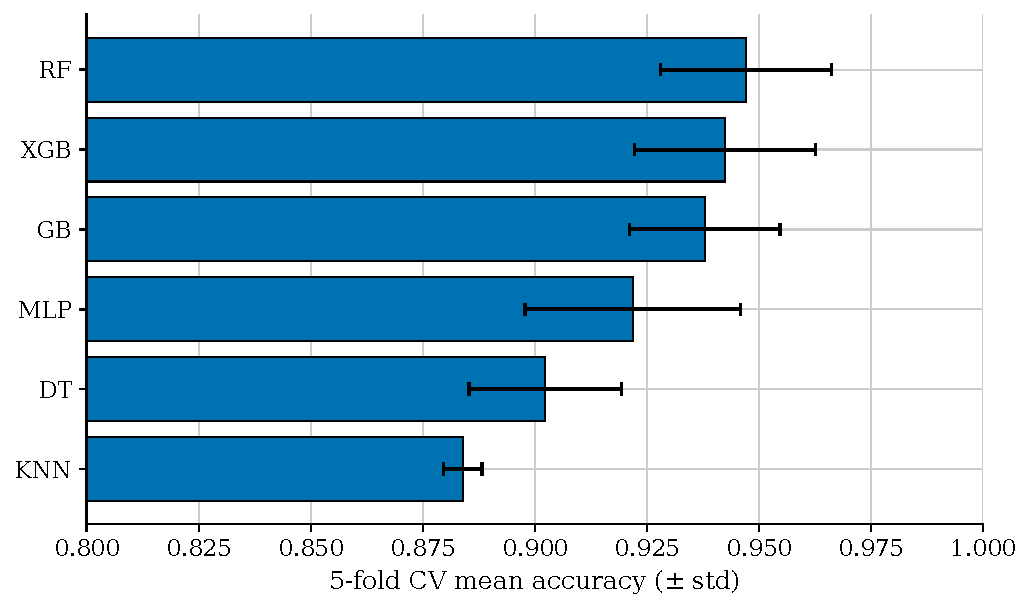
\includegraphics[width=0.85\textwidth]{figures/ch4/fig_ch4_algorithm_comparison.pdf}
\caption{Five-fold stratified cross-validation mean accuracy (± one standard deviation) for the six candidate algorithms, training split, ranked by CV mean. Source: \texttt{figures/ch4/fig\_ch4\_algorithm\_comparison}.}
\label{fig:ch4-algorithm-comparison}
\end{figure}

Three observations.

The \textbf{ranking reproduces the reference study's ordering} in its essentials. Polenta et al.~{[}5{]} found random forest strongest, gradient-boosted trees second, and kNN weakest among their six candidates; the same ordering appears here, with XGBoost occupying the position their SVM held. That an independent implementation on a different protocol recovers the same ranking is modest evidence that the ordering reflects a property of the data rather than of either implementation.

The \textbf{top three are closely spaced}. RF, XGB and GB span 0.9379 to 0.9471 --- a range of 0.0092, which is smaller than the cross-validation standard deviation of any of the three. As anticipated in §3.4.4, the defensible reading is that these three are effectively indistinguishable on this dataset, and the claim made here is that Random Forest is an appropriate champion, not that it is uniquely correct.

The \textbf{two criteria disagree}, exactly as §3.4.4 anticipated. XGBoost attains the highest single-split validation accuracy (0.9414 against RF's 0.9310), while Random Forest attains the highest cross-validation mean. The gap on the validation split is 0.0104, or approximately three samples out of 290 --- a difference at the resolution of sampling noise. Selection proceeded on CV mean, and Random Forest is the champion. Had the single split been used, the entire downstream chain would have been built on a different model on the basis of three samples.

kNN's very low CV standard deviation (0.0043) is worth a note: it is the most \emph{consistent} model and the least \emph{accurate}, a reminder that stability and performance are separate properties.

\hypertarget{champion-performance-on-the-held-out-test-split}{%
\subsection{4.2.2 Champion Performance on the Held-Out Test Split}\label{champion-performance-on-the-held-out-test-split}}

The champion Random Forest was evaluated once on the held-out test split, which participated in no selection decision.

\textbf{Table 4.4.} Champion model performance on the held-out test split. Source: \texttt{models/test\_evaluation.json}.

\begin{longtable}[]{@{}
  >{\raggedright\arraybackslash}p{(\columnwidth - 12\tabcolsep) * \real{0.1429}}
  >{\raggedright\arraybackslash}p{(\columnwidth - 12\tabcolsep) * \real{0.1429}}
  >{\raggedright\arraybackslash}p{(\columnwidth - 12\tabcolsep) * \real{0.1429}}
  >{\raggedright\arraybackslash}p{(\columnwidth - 12\tabcolsep) * \real{0.1429}}
  >{\raggedright\arraybackslash}p{(\columnwidth - 12\tabcolsep) * \real{0.1429}}
  >{\raggedright\arraybackslash}p{(\columnwidth - 12\tabcolsep) * \real{0.1429}}
  >{\raggedright\arraybackslash}p{(\columnwidth - 12\tabcolsep) * \real{0.1429}}@{}}
\toprule\noalign{}
\begin{minipage}[b]{\linewidth}\raggedright
Model
\end{minipage} & \begin{minipage}[b]{\linewidth}\raggedright
N samples
\end{minipage} & \begin{minipage}[b]{\linewidth}\raggedright
Accuracy
\end{minipage} & \begin{minipage}[b]{\linewidth}\raggedright
F1 (weighted)
\end{minipage} & \begin{minipage}[b]{\linewidth}\raggedright
F1 (macro)
\end{minipage} & \begin{minipage}[b]{\linewidth}\raggedright
Non-conformance precision
\end{minipage} & \begin{minipage}[b]{\linewidth}\raggedright
Non-conformance recall
\end{minipage} \\
\midrule\noalign{}
\endhead
\bottomrule\noalign{}
\endlastfoot
RandomForestClassifier & 291 & 0.9381 & 0.9381 & 0.9369 & 0.9329 & 0.9456 \\
\end{longtable}

Headline test accuracy is \textbf{93.81\%} on 291 held-out samples. Weighted and macro F1 are 0.9381 and 0.9369 respectively; their near-equality reflects the balanced class distribution established in §3.2.4 and indicates that performance is not being carried by a majority class.

Test accuracy (93.81\%) is 0.90 percentage points below the cross-validation mean (94.71\%) and 0.71 points above validation accuracy (93.10\%). The relationship among the three is unremarkable and is what a well-behaved model on a modest dataset should produce: no evidence of overfitting to the training split, and no evidence that the validation split was anomalously easy or hard.

\textbf{Non-conformance recall is 94.56\%.} This is the operationally central figure identified in §3.9.1: of all genuinely non-conforming cycles in the test split, the model correctly identifies 94.56\% as non-conforming. Non-conformance precision is 93.29\%, so the screening function is roughly symmetric in its error profile.

\hypertarget{per-class-precision-and-recall}{%
\subsection{4.2.3 Per-Class Precision and Recall}\label{per-class-precision-and-recall}}

\textbf{Table 4.5.} Per-class precision, recall, and support on the held-out test split (n = 291). Source: \texttt{models/test\_evaluation.json}.

\begin{longtable}[]{@{}llll@{}}
\toprule\noalign{}
Class & Precision & Recall & Support \\
\midrule\noalign{}
\endhead
\bottomrule\noalign{}
\endlastfoot
Waste & 0.9459 & 0.9459 & 74 \\
Acceptable & 0.9512 & 0.9512 & 82 \\
Target & 0.9333 & 0.9032 & 62 \\
Inefficient & 0.9200 & 0.9452 & 73 \\
\end{longtable}

\textbf{Recall on the safety-critical \emph{Waste} class is 94.59\%.} Of 74 truly non-compliant lenses in the test split, 70 are correctly identified and 4 are not. Precision on the same class is identical at 94.59\%, so the model is neither systematically over- nor under-calling \emph{Waste}.

The weakest cell in the table is \textbf{recall on \emph{Target} (90.32\%)}, the only value below 0.92. Six of 62 \emph{Target} cycles are missed. The consequence is benign: as the confusion matrix below shows, all six are misclassified as \emph{Inefficient}, which is a confusion between two classes that are both compliant with UNI EN 13201-2:2016. A \emph{Target} part called \emph{Inefficient} is still a saleable part; the error costs a spurious efficiency signal, not a customer defect. The reference study reaches the same conclusion about the relative severity of confusions within the compliant region.

Precision on \emph{Inefficient} (92.00\%) is the lowest precision figure and is the mirror image of the same phenomenon: the class absorbs the six misrouted \emph{Target} cycles.

\hypertarget{confusion-matrix}{%
\subsection{4.2.4 Confusion Matrix}\label{confusion-matrix}}

\textbf{Table 4.6.} Confusion matrix on the held-out test split (n = 291), with row and column totals. Rows are true classes, columns predicted. Source: \texttt{models/test\_evaluation.json}.

\begin{longtable}[]{@{}
  >{\raggedright\arraybackslash}p{(\columnwidth - 10\tabcolsep) * \real{0.1667}}
  >{\raggedright\arraybackslash}p{(\columnwidth - 10\tabcolsep) * \real{0.1667}}
  >{\raggedright\arraybackslash}p{(\columnwidth - 10\tabcolsep) * \real{0.1667}}
  >{\raggedright\arraybackslash}p{(\columnwidth - 10\tabcolsep) * \real{0.1667}}
  >{\raggedright\arraybackslash}p{(\columnwidth - 10\tabcolsep) * \real{0.1667}}
  >{\raggedright\arraybackslash}p{(\columnwidth - 10\tabcolsep) * \real{0.1667}}@{}}
\toprule\noalign{}
\begin{minipage}[b]{\linewidth}\raggedright
True ~Predicted
\end{minipage} & \begin{minipage}[b]{\linewidth}\raggedright
Waste
\end{minipage} & \begin{minipage}[b]{\linewidth}\raggedright
Acceptable
\end{minipage} & \begin{minipage}[b]{\linewidth}\raggedright
Target
\end{minipage} & \begin{minipage}[b]{\linewidth}\raggedright
Inefficient
\end{minipage} & \begin{minipage}[b]{\linewidth}\raggedright
Row total
\end{minipage} \\
\midrule\noalign{}
\endhead
\bottomrule\noalign{}
\endlastfoot
\textbf{Waste} & 70 & 4 & 0 & 0 & 74 \\
\textbf{Acceptable} & 4 & 78 & 0 & 0 & 82 \\
\textbf{Target} & 0 & 0 & 56 & 6 & 62 \\
\textbf{Inefficient} & 0 & 0 & 4 & 69 & 73 \\
\textbf{Column total} & 74 & 82 & 60 & 75 & 291 \\
\end{longtable}

\begin{figure}[htbp]
\centering
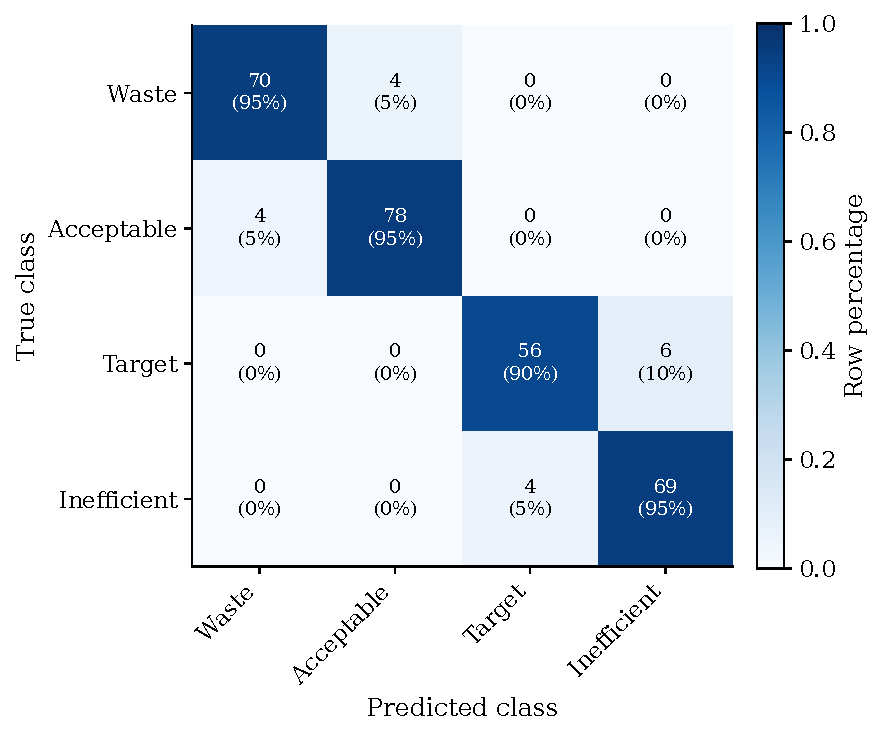
\includegraphics[width=0.75\textwidth]{figures/ch4/fig_ch4_confusion_matrix_test.pdf}
\caption{Confusion matrix of the champion model on the held-out test split (n = 291), annotated with raw counts and row-normalised percentages. Source: \texttt{figures/ch4/fig\_ch4\_confusion\_matrix\_test}.}
\label{fig:ch4-confusion-matrix-test}
\end{figure}

The matrix has a striking and analytically important structure: \textbf{it is block-diagonal.} All 18 errors fall within one of two adjacent-class blocks --- \{\emph{Waste}, \emph{Acceptable}\} accounts for 8 errors, and \{\emph{Target}, \emph{Inefficient}\} accounts for 10 --- and the two blocks do not exchange a single sample. There is no cycle anywhere in the test split that the model confuses across the \{\emph{Waste}, \emph{Acceptable}\} / \{\emph{Target}, \emph{Inefficient}\} boundary.

This means the model's errors follow the ordinal structure of the underlying photometric measurement. The four classes are ordered bands of general uniformity U\textsubscript{0}, and every error the model makes is a confusion between adjacent bands. It never mistakes a badly under-performing lens for an over-performing one. For a quality-control application this is close to the best available error structure, because it means the \emph{magnitude} of every error is bounded by one band.

The safety-critical cell is the \emph{Waste} → \emph{Acceptable} off-diagonal: \textbf{4 of 291 test cycles (1.37\%)} are non-compliant lenses that the model would pass. The mirror cell, \emph{Acceptable} → \emph{Waste}, is also 4, so 4 compliant lenses would be scrapped unnecessarily. The two error types are exactly balanced at this operating point, which is a consequence of the model's calibration on a balanced dataset rather than of any deliberate cost weighting. §5.1 discusses whether a production deployment should shift this balance by adjusting the decision threshold in favour of \emph{Waste} recall, accepting more spurious scrap in exchange for fewer escapes.

\hypertarget{comparison-with-the-reference-benchmark}{%
\subsection{4.2.5 Comparison with the Reference Benchmark}\label{comparison-with-the-reference-benchmark}}

\textbf{Table 4.7.} Per-class comparison against Polenta et al.~{[}5{]}, Table 10, Random Forest row. \textbf{Protocol difference:} this work reports a single held-out test split (n = 291); the reference reports samples summed across the five folds of stratified five-fold cross-validation over the full 1,451-sample dataset. The two are not a like-for-like comparison. Source: \texttt{models/test\_evaluation.json} and the \texttt{POLENTA\_TABLE10\_RF} constant.

\begin{longtable}[]{@{}
  >{\raggedright\arraybackslash}p{(\columnwidth - 8\tabcolsep) * \real{0.2000}}
  >{\raggedright\arraybackslash}p{(\columnwidth - 8\tabcolsep) * \real{0.2000}}
  >{\raggedright\arraybackslash}p{(\columnwidth - 8\tabcolsep) * \real{0.2000}}
  >{\raggedright\arraybackslash}p{(\columnwidth - 8\tabcolsep) * \real{0.2000}}
  >{\raggedright\arraybackslash}p{(\columnwidth - 8\tabcolsep) * \real{0.2000}}@{}}
\toprule\noalign{}
\begin{minipage}[b]{\linewidth}\raggedright
Class
\end{minipage} & \begin{minipage}[b]{\linewidth}\raggedright
This work: precision (test, n = 291)
\end{minipage} & \begin{minipage}[b]{\linewidth}\raggedright
Reference: precision (5-fold CV, n = 1451)
\end{minipage} & \begin{minipage}[b]{\linewidth}\raggedright
This work: recall (test, n = 291)
\end{minipage} & \begin{minipage}[b]{\linewidth}\raggedright
Reference: recall (5-fold CV, n = 1451)
\end{minipage} \\
\midrule\noalign{}
\endhead
\bottomrule\noalign{}
\endlastfoot
Waste & 0.9459 & 0.9722 & 0.9459 & 0.9459 \\
Acceptable & 0.9512 & 0.9511 & 0.9512 & 0.9581 \\
Target & 0.9333 & 0.9437 & 0.9032 & 0.9194 \\
Inefficient & 0.9200 & 0.9342 & 0.9452 & 0.9736 \\
\end{longtable}

\begin{figure}[htbp]
\centering
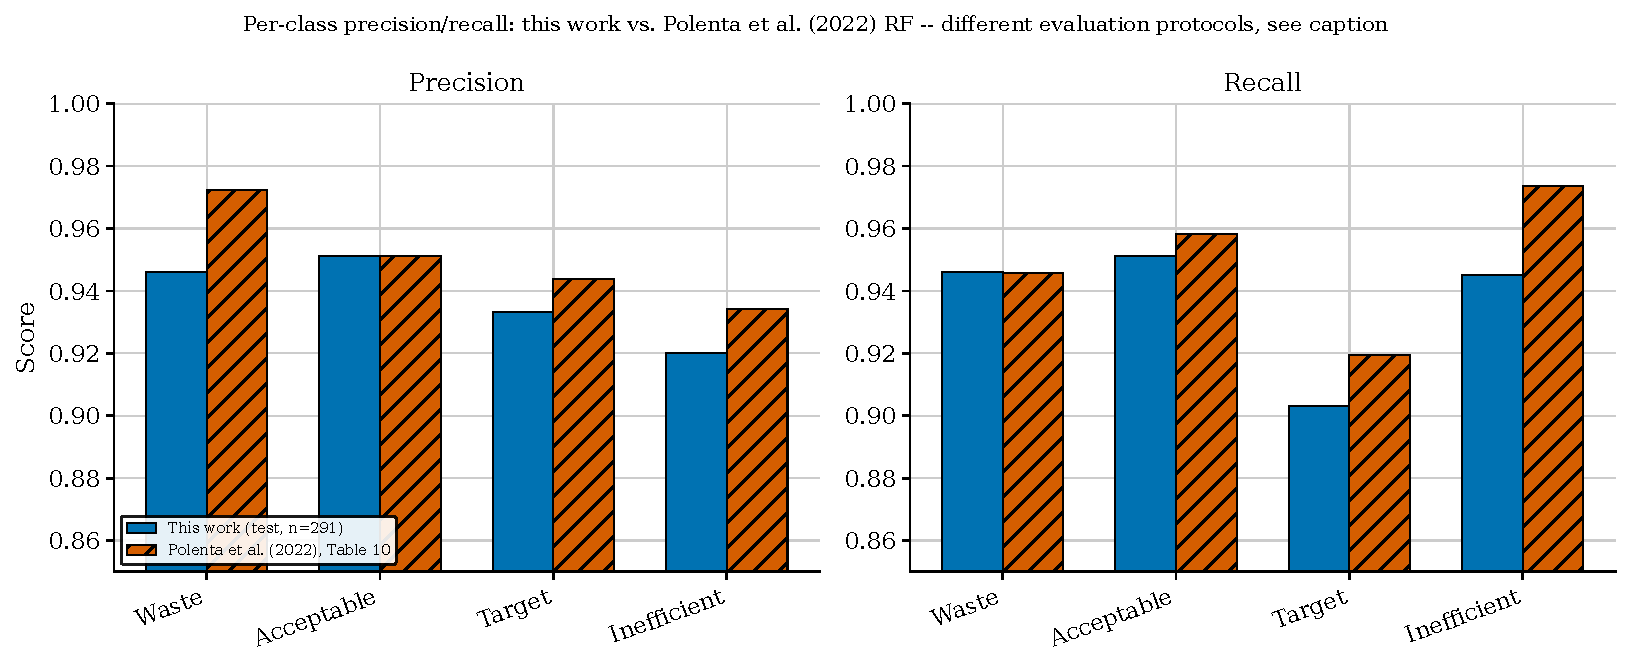
\includegraphics[width=0.85\textwidth]{figures/ch4/fig_ch4_per_class_vs_baseline.pdf}
\caption{Per-class precision and recall on this work's held-out test split against the Random Forest row of the reference study. Protocol difference noted in the figure. Source: \texttt{figures/ch4/fig\_ch4\_per\_class\_vs\_baseline}.}
\label{fig:ch4-per-class-vs-baseline}
\end{figure}

At aggregate level, the reference reports 95.04\% ± 1.26\% mean accuracy from five-fold cross-validation over all 1,451 samples; this work reports 93.81\% on a held-out split of 291.

\textbf{These figures are not directly comparable, and no claim of parity or superiority is made.} The reason was set out in §3.4.3, deviation §5, and bears restating at the point of comparison. The reference's protocol averages over five folds in which every sample appears in a test fold exactly once, so its denominator is the full dataset and each of its estimates is trained on 80\% of the data. This work's figure comes from a single split of 291 samples with a model trained on 60\% of the data. The reference's figure is an average over more data, trained on more data; this work's is a single estimate on less data, trained on less. A difference of 1.23 percentage points between them carries no interpretable meaning.

What the comparison does support is a weaker but useful statement: \textbf{the per-class profile is consistent between the two.} Recall on \emph{Waste} is essentially identical (0.9459 in both). Precision on \emph{Acceptable} matches to four decimal places (0.9512 versus 0.9511), which is coincidental in its exactness but indicative in its closeness. The reference is uniformly slightly higher on the remaining cells, in the direction its protocol advantage predicts. Nothing in the comparison suggests that the adopted hyperparameter configuration --- with the five deviations documented in §3.4.3 --- has produced a materially different model from the one the reference describes.

This is the appropriate conclusion for a reproduction: not that the result was matched or beaten, but that the reimplementation behaves like the thing it reimplements. That is what licenses using this model as the substrate for the counterfactual work that follows.

\begin{center}\rule{0.5\linewidth}{0.5pt}\end{center}

\hypertarget{explanation-layer-results}{%
\section{4.3 Explanation Layer Results}\label{explanation-layer-results}}

\hypertarget{global-shap-feature-importance}{%
\subsection{4.3.1 Global SHAP Feature Importance}\label{global-shap-feature-importance}}

Global attributions were computed by TreeSHAP over the full training split and aggregated as mean absolute SHAP value per feature across all four classes.

\textbf{Table 4.8.} All 13 process parameters ranked by mean absolute SHAP value, aggregated across classes, training split. Source: \texttt{thesis\_assets/data/shap\_global\_importance.json}.

\begin{longtable}[]{@{}lll@{}}
\toprule\noalign{}
Rank & Parameter & Mean \textbar SHAP\textbar{} \\
\midrule\noalign{}
\endhead
\bottomrule\noalign{}
\endlastfoot
1 & ZUx -- Cycle time & 0.09987 \\
2 & ZDx -- Plasticizing time & 0.06997 \\
3 & time\_to\_fill & 0.05219 \\
4 & SKx -- Closing force & 0.04128 \\
5 & APVs -- Specific injection pressure peak value & 0.04110 \\
6 & SKs -- Clamping force peak value & 0.03640 \\
7 & Mold temperature & 0.03082 \\
8 & Melt temperature & 0.01494 \\
9 & CPn -- Screw position at end of hold pressure & 0.01313 \\
10 & SVo -- Shot volume & 0.01124 \\
11 & Mm -- Torque mean value & 0.00750 \\
12 & Ms -- Torque peak value & 0.00570 \\
13 & APSs -- Specific back pressure peak value & 0.00331 \\
\end{longtable}

\begin{figure}[htbp]
\centering
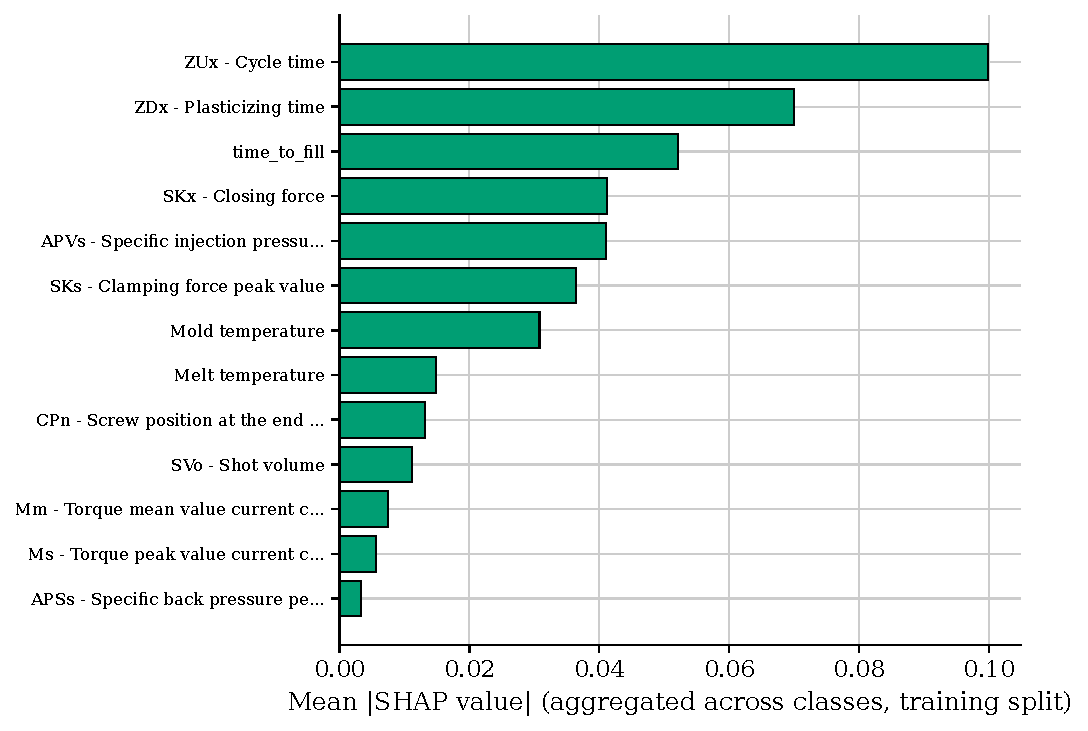
\includegraphics[width=0.85\textwidth]{figures/ch4/fig_ch4_shap_global_bar.pdf}
\caption{Global feature importance from SHAP TreeExplainer, mean absolute SHAP value per parameter over the full training split, aggregated across all four classes. Source: \texttt{figures/ch4/fig\_ch4\_shap\_global\_bar}.}
\label{fig:ch4-shap-global-bar}
\end{figure}

\begin{figure}[htbp]
\centering
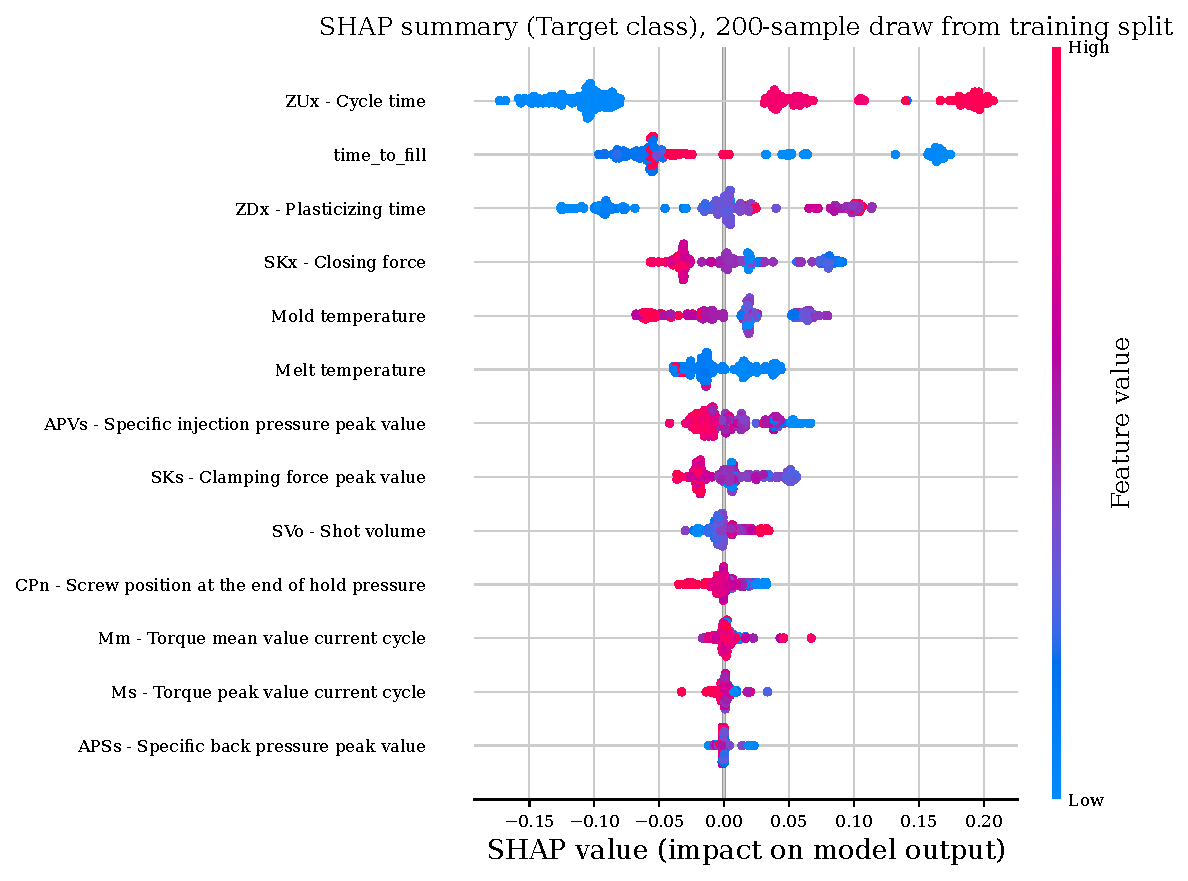
\includegraphics[width=0.85\textwidth]{figures/ch4/fig_ch4_shap_beeswarm.pdf}
\caption{SHAP summary (beeswarm) plot for the \emph{Target} class, computed on a 200-sample random draw from the training split (seed 42). Colour encodes feature value; horizontal position encodes signed SHAP contribution. Source: \texttt{figures/ch4/fig\_ch4\_shap\_beeswarm}.}
\label{fig:ch4-shap-beeswarm}
\end{figure}

The ranking is dominated by \textbf{time-domain parameters}. The top three --- cycle time, plasticizing time, and filling time --- are all durations, and together they carry more attribution mass than the remaining ten parameters combined. Cycle time alone (0.09987) is worth more than the bottom seven parameters together. The force and pressure group occupies ranks 4 to 6, temperatures ranks 7 to 8, and the torque and back-pressure measurements are close to irrelevant to the model at ranks 11 to 13.

This is a substantive statement about the process rather than an artefact of the model, and §5.1 develops its physical interpretation. Its immediate consequence for the present chapter is that the Tier-1 counterfactual search, which selects the top five features by local \textbar SHAP\textbar, will predominantly be adjusting timings --- which is precisely what §4.4.3 shows.

\hypertarget{agreement-with-independent-importance-methods}{%
\subsection{4.3.2 Agreement with Independent Importance Methods}\label{agreement-with-independent-importance-methods}}

Because §2.7 argues that a model's endorsement of its own explanation is weak evidence, the global ranking was compared against three other importance methods: the model's own impurity-based importances, and the Relief and ANOVA filter weights reported by the reference study for the same dataset.

\textbf{Table 4.9.} Importance comparison across four methods for all 13 parameters, with Spearman rank correlations. Relief and ANOVA weights reproduced from Polenta et al.~{[}5{]}, Figures 2--3; they are reference constants, not values computed in this work. Source: \texttt{thesis\_assets/data/shap\_vs\_impurity.json}, \texttt{shap\_vs\_filters.json}.

\begin{longtable}[]{@{}
  >{\raggedright\arraybackslash}p{(\columnwidth - 10\tabcolsep) * \real{0.1667}}
  >{\raggedright\arraybackslash}p{(\columnwidth - 10\tabcolsep) * \real{0.1667}}
  >{\raggedright\arraybackslash}p{(\columnwidth - 10\tabcolsep) * \real{0.1667}}
  >{\raggedright\arraybackslash}p{(\columnwidth - 10\tabcolsep) * \real{0.1667}}
  >{\raggedright\arraybackslash}p{(\columnwidth - 10\tabcolsep) * \real{0.1667}}
  >{\raggedright\arraybackslash}p{(\columnwidth - 10\tabcolsep) * \real{0.1667}}@{}}
\toprule\noalign{}
\begin{minipage}[b]{\linewidth}\raggedright
Parameter (reference name)
\end{minipage} & \begin{minipage}[b]{\linewidth}\raggedright
Column
\end{minipage} & \begin{minipage}[b]{\linewidth}\raggedright
SHAP
\end{minipage} & \begin{minipage}[b]{\linewidth}\raggedright
Impurity
\end{minipage} & \begin{minipage}[b]{\linewidth}\raggedright
Relief
\end{minipage} & \begin{minipage}[b]{\linewidth}\raggedright
ANOVA
\end{minipage} \\
\midrule\noalign{}
\endhead
\bottomrule\noalign{}
\endlastfoot
cycle time & ZUx -- Cycle time & 0.09987 & 0.21133 & 1.0000 & 1.0000 \\
plasticizing time & ZDx -- Plasticizing time & 0.06997 & 0.16520 & 0.0913 & 0.0199 \\
filling time & time\_to\_fill & 0.05219 & 0.11838 & 0.5749 & 0.0250 \\
closing force & SKx -- Closing force & 0.04128 & 0.10011 & 0.1793 & 0.0145 \\
specific injection pressure & APVs -- Spec. inj. pressure peak & 0.04110 & 0.08976 & 0.0632 & 0.0295 \\
clamping force & SKs -- Clamping force peak & 0.03640 & 0.08627 & 0.1849 & 0.0101 \\
mold temperature & Mold temperature & 0.03082 & 0.07872 & 0.1325 & 0.0289 \\
melt temperature & Melt temperature & 0.01494 & 0.04200 & 0.0000 & 0.0000 \\
screw position & CPn -- Screw position & 0.01313 & 0.03064 & 0.1421 & 0.0202 \\
shot volume & SVo -- Shot volume & 0.01124 & 0.02833 & 0.1393 & 0.0204 \\
torque mean & Mm -- Torque mean & 0.00750 & 0.02320 & 0.0584 & 0.0020 \\
torque peak & Ms -- Torque peak & 0.00570 & 0.01609 & 0.0611 & 0.0012 \\
specific back pressure & APSs -- Spec. back pressure peak & 0.00331 & 0.00998 & 0.0038 & 0.0032 \\
\textbf{Spearman r (SHAP vs.~impurity)} & & \textbf{1.0000} & \emph{p} = 0.0 & & \\
\textbf{Spearman r (SHAP vs.~Relief)} & & \textbf{0.6593} & \emph{p} = 0.0142 & & \\
\textbf{Spearman r (SHAP vs.~ANOVA)} & & \textbf{0.6044} & \emph{p} = 0.0287 & & \\
\end{longtable}

\begin{figure}[htbp]
\centering
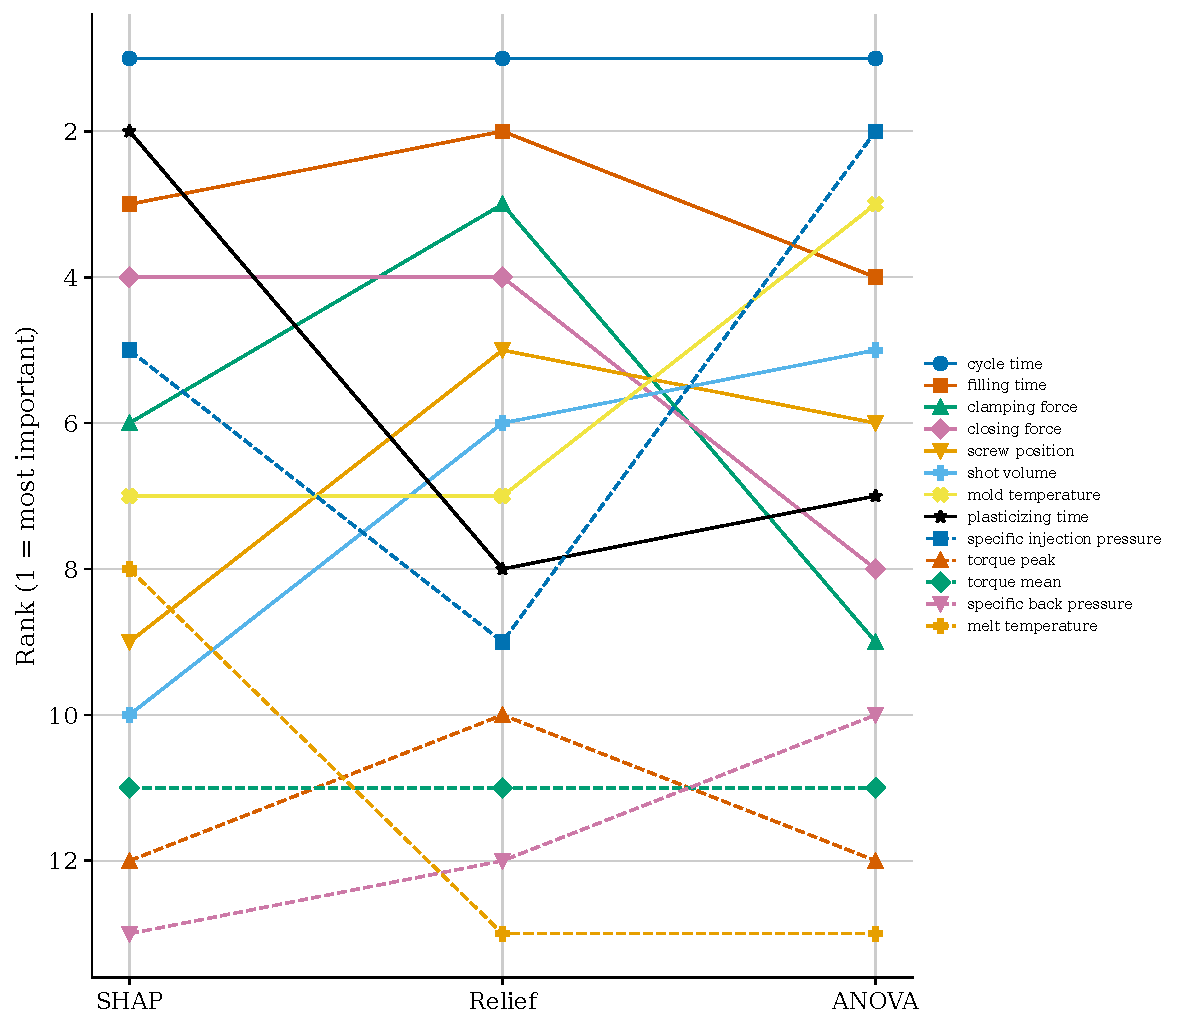
\includegraphics[width=0.85\textwidth]{figures/ch4/fig_ch4_importance_method_comparison.pdf}
\caption{Rank comparison of the 13 parameters across SHAP (this work, training split) and the Relief and ANOVA filter rankings reported in the reference study. Source: \texttt{figures/ch4/fig\_ch4\_importance\_method\_comparison}.}
\label{fig:ch4-importance-method-comparison}
\end{figure}

Three findings, of decreasing strength.

\textbf{SHAP and impurity importance agree perfectly in rank (Spearman r = 1.000).} All 13 parameters occupy identical positions under both methods. This is a reassuring internal-consistency result --- the exact Shapley attribution and the model's own splitting statistics tell the same story about which parameters the forest relies on --- but it must not be over-read. Both quantities are computed from the same fitted model, so their agreement is agreement of a model with itself. It establishes that the SHAP implementation is behaving correctly; it establishes nothing about the process.

\textbf{SHAP agrees moderately with the two independent filter methods} (r = 0.659 against Relief, \emph{p} = 0.014; r = 0.604 against ANOVA, \emph{p} = 0.029). Both correlations are positive and statistically significant at α = 0.05. This is the more meaningful comparison, because Relief and ANOVA are computed from the data without reference to any trained model, so agreement between them and SHAP is agreement between a model-derived and a model-free account of what matters.

\textbf{All three methods rank cycle time first.} This is the single most robust finding of the explanation layer: three methodologically unrelated procedures --- an exact game-theoretic attribution over a random forest, a nearest-neighbour-based filter, and a univariate analysis of variance --- independently identify the same parameter as most informative.

The disagreements are also informative and should not be smoothed over. Relief ranks filling time second (0.5749) where SHAP ranks it third and ANOVA ranks it fourth. More strikingly, both filter methods assign melt temperature a weight of exactly 0.0 --- no univariate discriminative power at all --- while SHAP places it eighth of thirteen with a non-trivial attribution. The most plausible explanation is that melt temperature carries information only in interaction with other parameters, which a univariate filter cannot see and a tree ensemble can. This is a small illustration of the disagreement problem documented by Krishna et al.~{[}73{]} and observed in injection molding by Muaz et al.~{[}47{]}, and it is exactly why §3.9.2 requires reporting agreement rather than asserting correctness.

\hypertarget{local-explanations-and-shaplime-agreement}{%
\subsection{4.3.3 Local Explanations and SHAP--LIME Agreement}\label{local-explanations-and-shaplime-agreement}}

Local explanations were computed for three worked test-split cases, chosen as one correctly classified instance of each outcome of interest: a \emph{Waste} cycle (test index 8), an \emph{Inefficient} cycle (test index 5), and a \emph{Target} cycle (test index 0).

\begin{figure}[htbp]
\centering
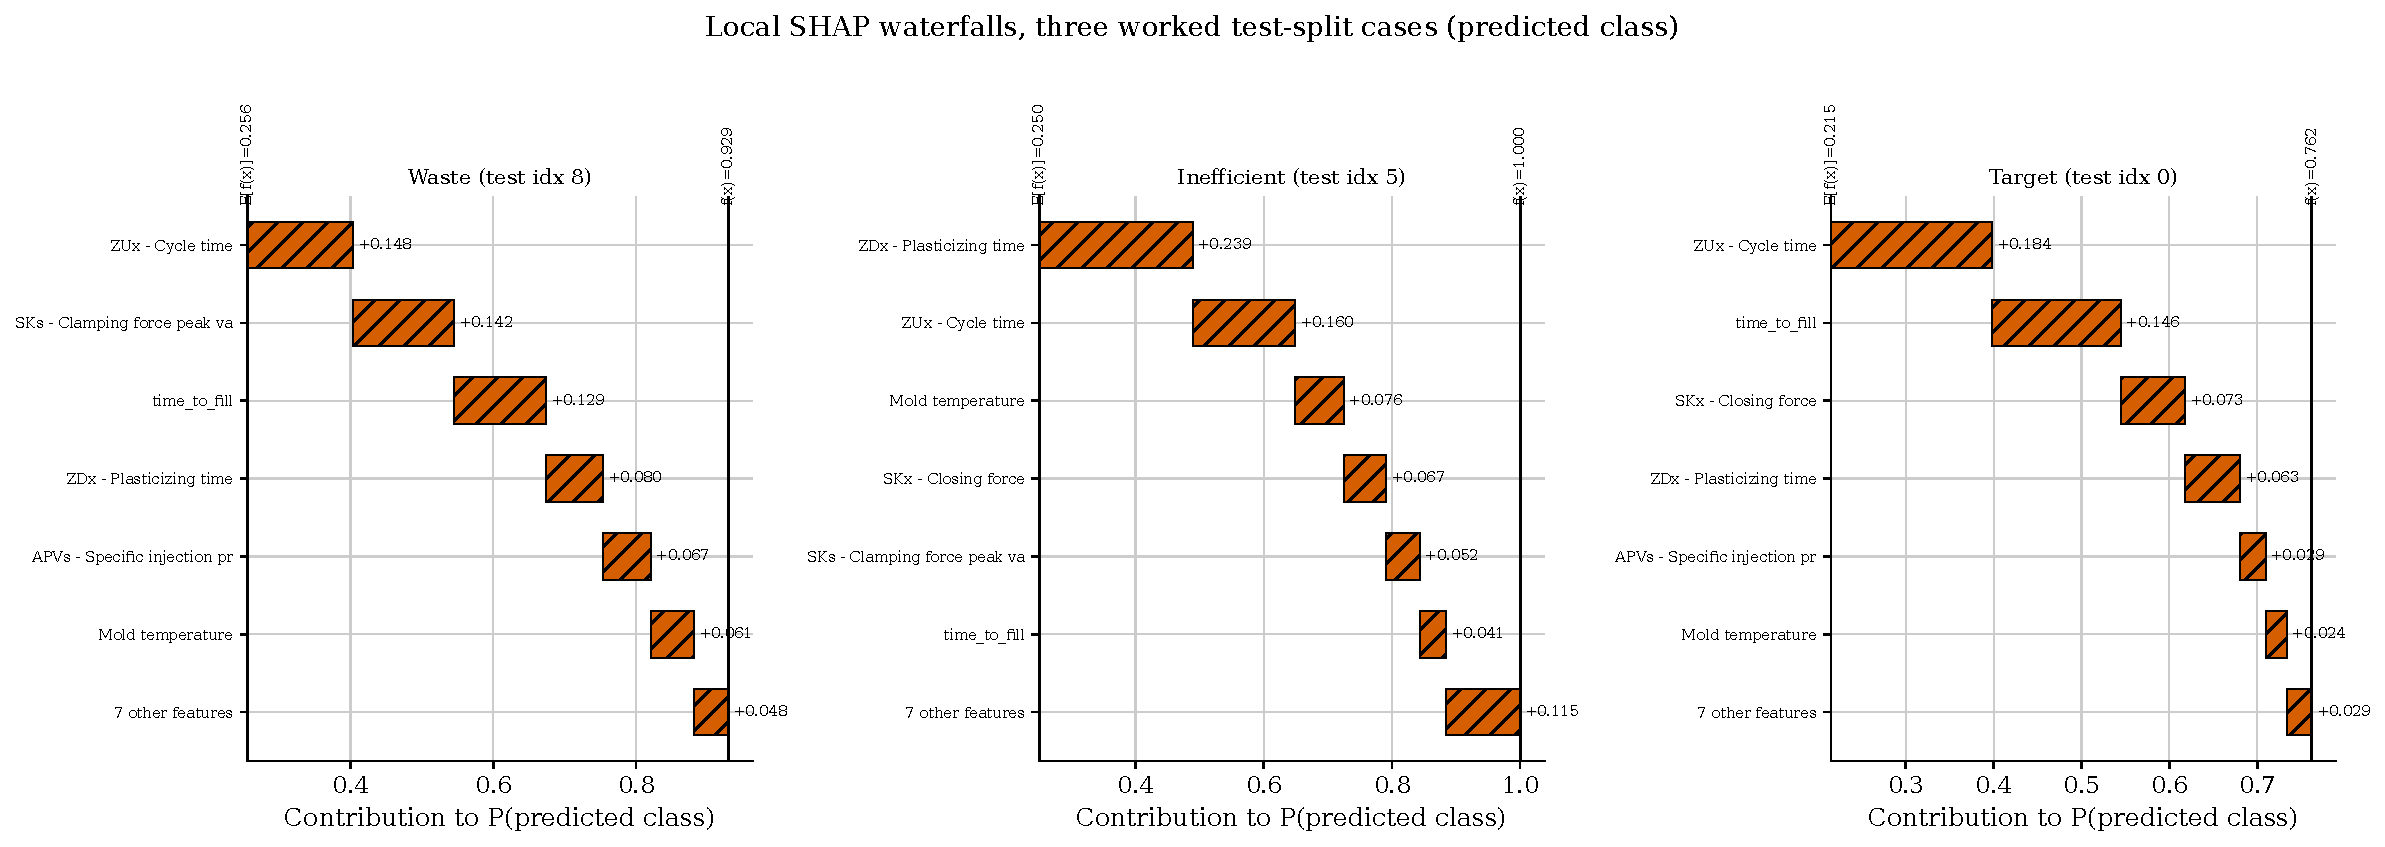
\includegraphics[width=0.85\textwidth]{figures/ch4/fig_ch4_shap_local_waterfall.pdf}
\caption{Local SHAP explanations for the three worked test-split cases, decomposing the predicted-class probability from the SHAP expected value to the realised prediction, largest contributions first. Source: \texttt{figures/ch4/fig\_ch4\_shap\_local\_waterfall}, \texttt{thesis\_assets/data/local\_explanations.json}.}
\label{fig:ch4-shap-local-waterfall}
\end{figure}

\begin{figure}[htbp]
\centering
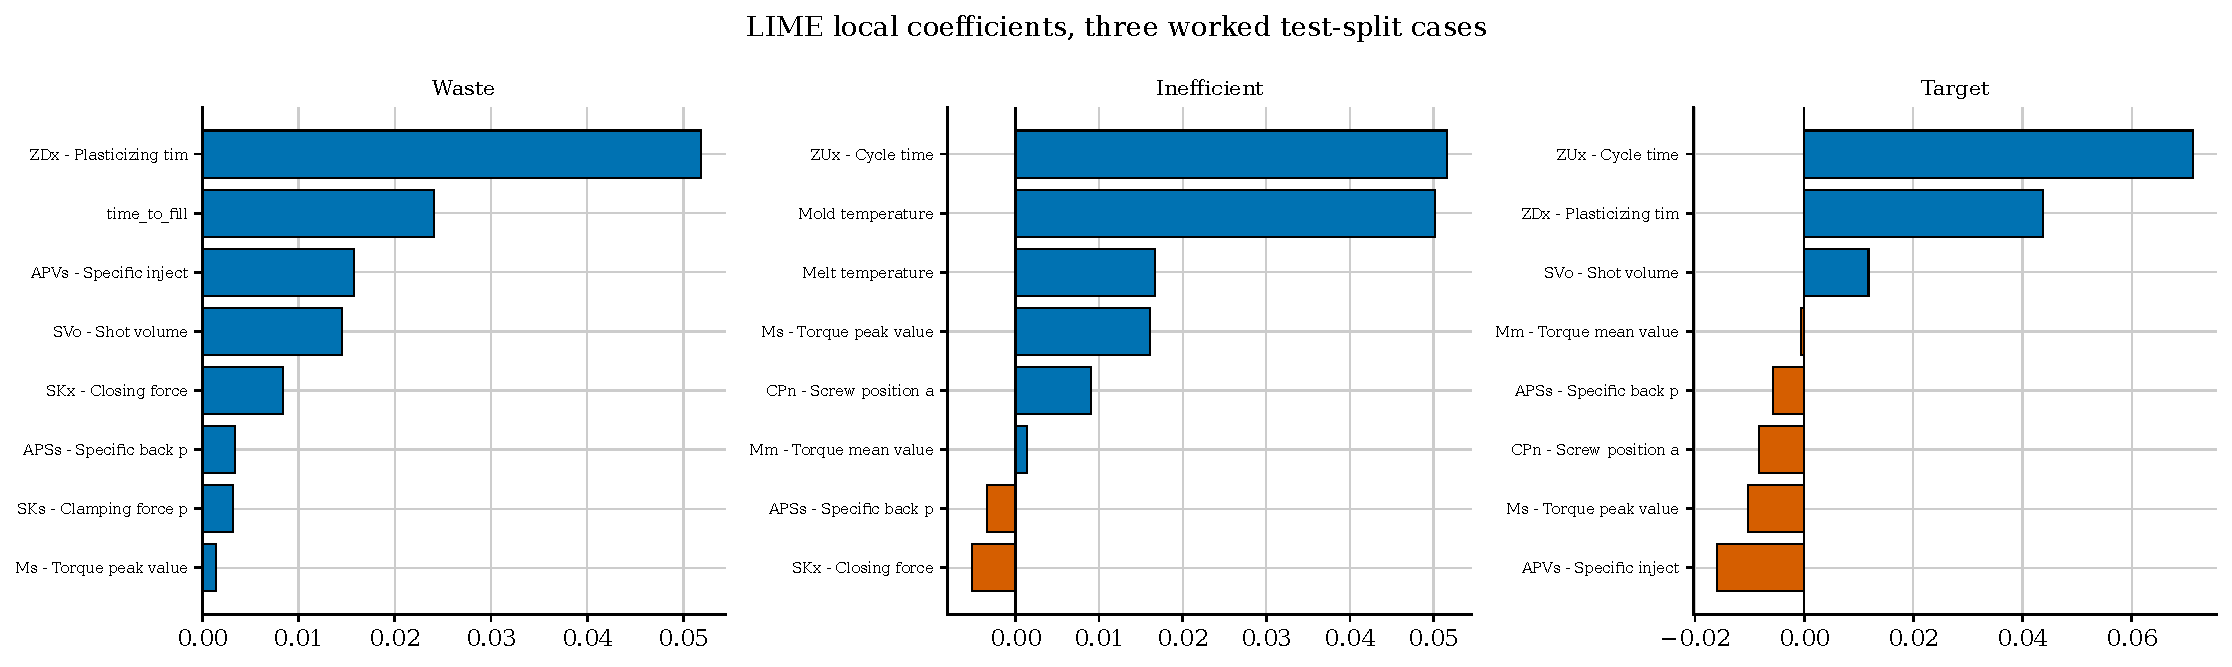
\includegraphics[width=0.85\textwidth]{figures/ch4/fig_ch4_lime_local.pdf}
\caption{LIME local linear coefficients for the same three cases, for direct comparison on identical cycles. Source: \texttt{figures/ch4/fig\_ch4\_lime\_local}.}
\label{fig:ch4-lime-local}
\end{figure}

Because the counterfactual engine depends on SHAP and LIME performing different jobs on the same cycle (§3.5.3), the degree to which they agree is a precondition for the design being coherent. Agreement was measured over 50 randomly drawn test-split cycles by ranking all 13 parameters under each method and computing the Spearman rank correlation, together with the overlap of the two top-five sets.

\textbf{Table 4.10.} SHAP--LIME rank agreement over 50 randomly drawn test-split cycles. Source: \texttt{thesis\_assets/data/shap\_lime\_agreement.json}.

\begin{longtable}[]{@{}
  >{\raggedright\arraybackslash}p{(\columnwidth - 2\tabcolsep) * \real{0.5000}}
  >{\raggedright\arraybackslash}p{(\columnwidth - 2\tabcolsep) * \real{0.5000}}@{}}
\toprule\noalign{}
\begin{minipage}[b]{\linewidth}\raggedright
Measure
\end{minipage} & \begin{minipage}[b]{\linewidth}\raggedright
Value
\end{minipage} \\
\midrule\noalign{}
\endhead
\bottomrule\noalign{}
\endlastfoot
Mean Spearman r (SHAP rank vs.~LIME rank) & \emph{{[}Insert \texttt{spearman\_r\_mean} from artefact{]}} \\
Std. dev. of Spearman r & \emph{{[}Insert \texttt{spearman\_r\_std}{]}} \\
Mean top-5 overlap (of 5) & \emph{{[}Insert \texttt{top5\_overlap\_mean}{]}} \\
Std. dev. of top-5 overlap & \emph{{[}Insert \texttt{top5\_overlap\_std}{]}} \\
\end{longtable}

LIME's repeatability was assessed separately by re-running the explainer ten times on a single fixed test cycle, deliberately bypassing the result cache so that each run performs fresh stochastic perturbation sampling.

\textbf{Table 4.11.} LIME repeatability across ten independent runs on one fixed test-split cycle. Source: \texttt{thesis\_assets/data/lime\_stability.json}.

\begin{longtable}[]{@{}
  >{\raggedright\arraybackslash}p{(\columnwidth - 2\tabcolsep) * \real{0.5000}}
  >{\raggedright\arraybackslash}p{(\columnwidth - 2\tabcolsep) * \real{0.5000}}@{}}
\toprule\noalign{}
\begin{minipage}[b]{\linewidth}\raggedright
Measure
\end{minipage} & \begin{minipage}[b]{\linewidth}\raggedright
Value
\end{minipage} \\
\midrule\noalign{}
\endhead
\bottomrule\noalign{}
\endlastfoot
Number of runs & 10 \\
Mean top-5 overlap with first run (of 5) & \emph{{[}Insert \texttt{top5\_overlap\_with\_first\_run\_mean}{]}} \\
Largest per-feature coefficient standard deviation & \emph{{[}Insert max of \texttt{coefficient\_std\_by\_feature}{]}} \\
\end{longtable}

Two things matter about these measurements, whichever way the numbers fall.

The \textbf{stability of the top-five set is the property the engine actually depends on}, not the stability of the coefficient magnitudes. Tier 1 uses LIME only for the \emph{sign} of each coefficient on five features that SHAP has already selected. Coefficient magnitude variation across runs is therefore tolerable; sign instability would not be, since it would make the recommended direction of adjustment non-deterministic.

\textbf{TreeSHAP contributes no stochastic variation at all.} Because it computes exact Shapley values rather than sampling them, repeated attribution of the same cycle returns bit-identical results. All variability in the explanation layer originates in LIME. This asymmetry is the practical justification for the division of labour: the component responsible for \emph{which} parameters to touch is deterministic, and only the component responsible for \emph{which way} is stochastic.

\hypertarget{computational-cost}{%
\subsection{4.3.4 Computational Cost}\label{computational-cost}}

\textbf{Table 4.12.} Explanation-layer wall-clock cost, measured on 15 unique test-split cycles with a freshly constructed engine so that the cache begins empty. Each cycle is queried twice in sequence, simulating an operator re-opening a previously viewed cycle. Source: \texttt{thesis\_assets/data/xai\_timing.json}.

\begin{longtable}[]{@{}ll@{}}
\toprule\noalign{}
Measure & Value \\
\midrule\noalign{}
\endhead
\bottomrule\noalign{}
\endlastfoot
SHAP calls timed & 15 \\
SHAP mean time per call & 0.00177 s (± 0.00023 s) \\
LIME calls timed & 30 \\
LIME mean time per call & 0.02015 s (± 0.02047 s) \\
Cache hits / misses & 15 / 15 \\
Cache hit rate & 50.0\% \\
\end{longtable}

TreeSHAP attributes a cycle in under 2 milliseconds --- fast enough that attribution imposes no meaningful constraint on any deployment scenario. LIME averages 20 milliseconds per call, an order of magnitude slower, with a standard deviation (0.02047 s) essentially equal to its mean. That equality is itself the signal: the distribution is bimodal, not noisy. Cache misses run the full 2,000-sample perturbation and regression; cache hits return a stored list in microseconds. Averaged over a session in which half the calls hit, the mean lands between the two modes.

The 50.0\% hit rate is a direct consequence of the measurement protocol --- each cycle is queried exactly twice, so one miss and one hit per cycle by construction --- and should not be read as an estimate of production hit rate, which depends entirely on how often operators revisit cycles.

Even at the uncached figure, the practical conclusion is unchanged: a full explanation of a single cycle costs on the order of tens of milliseconds, against an injection molding cycle time measured in tens of seconds. The explanation layer is not a bottleneck for per-cycle analysis.

\begin{center}\rule{0.5\linewidth}{0.5pt}\end{center}

\hypertarget{counterfactual-root-cause-analysis-results}{%
\section{4.4 Counterfactual Root-Cause Analysis Results}\label{counterfactual-root-cause-analysis-results}}

This section reports what the engine does at its default operating point (acceptance threshold 0.55, iteration budget 150). §4.5 then reports what happens when those results are independently checked.

\hypertarget{resolution-rates}{%
\subsection{4.4.1 Resolution Rates}\label{resolution-rates}}

\textbf{Table 4.13.} RCA tier counts, resolution rate, and validator agreement on both splits at the default configuration (threshold = 0.55, max\_iter = 150). Source: \texttt{models/rca\_evaluation\_\{val,test\}.json}.

\begin{longtable}[]{@{}
  >{\raggedright\arraybackslash}p{(\columnwidth - 14\tabcolsep) * \real{0.1250}}
  >{\raggedright\arraybackslash}p{(\columnwidth - 14\tabcolsep) * \real{0.1250}}
  >{\raggedright\arraybackslash}p{(\columnwidth - 14\tabcolsep) * \real{0.1250}}
  >{\raggedright\arraybackslash}p{(\columnwidth - 14\tabcolsep) * \real{0.1250}}
  >{\raggedright\arraybackslash}p{(\columnwidth - 14\tabcolsep) * \real{0.1250}}
  >{\raggedright\arraybackslash}p{(\columnwidth - 14\tabcolsep) * \real{0.1250}}
  >{\raggedright\arraybackslash}p{(\columnwidth - 14\tabcolsep) * \real{0.1250}}
  >{\raggedright\arraybackslash}p{(\columnwidth - 14\tabcolsep) * \real{0.1250}}@{}}
\toprule\noalign{}
\begin{minipage}[b]{\linewidth}\raggedright
Split
\end{minipage} & \begin{minipage}[b]{\linewidth}\raggedright
N non-conforming
\end{minipage} & \begin{minipage}[b]{\linewidth}\raggedright
Tier 1
\end{minipage} & \begin{minipage}[b]{\linewidth}\raggedright
Tier 2
\end{minipage} & \begin{minipage}[b]{\linewidth}\raggedright
Tier 3
\end{minipage} & \begin{minipage}[b]{\linewidth}\raggedright
Resolution rate
\end{minipage} & \begin{minipage}[b]{\linewidth}\raggedright
Validator confirmed
\end{minipage} & \begin{minipage}[b]{\linewidth}\raggedright
Validator rate
\end{minipage} \\
\midrule\noalign{}
\endhead
\bottomrule\noalign{}
\endlastfoot
val & 147 & 144 & 0 & 0 & 0.9796 & 16 & 0.1111 \\
\textbf{test} & \textbf{147} & \textbf{140} & \textbf{0} & \textbf{0} & \textbf{0.9524} & \textbf{9} & \textbf{0.0643} \\
\end{longtable}

On the held-out test split, the engine produces a counterfactual for \textbf{140 of 147 non-conforming cycles --- a resolution rate of 95.24\%.} On the validation split the figure is 144 of 147, or 97.96\%.

Read on its own, this is a strong result, and it is the result that a conventional counterfactual study would report as its headline. For 95\% of defective cycles, the engine returns a concrete set of parameter adjustments that moves the cycle into the conforming region as far as the champion model is concerned.

\textbf{The seven unresolved cases are not search failures.} This requires stating precisely at the point the figure appears, because the natural reading of 140/147 is that the search failed seven times, and that reading is wrong.

\textbf{Table 4.14.} Disposition of the seven test-split cycles excluded from the resolved count. Source: \texttt{thesis\_assets/data/unresolved\_analysis.json}.

\begin{longtable}[]{@{}
  >{\raggedright\arraybackslash}p{(\columnwidth - 6\tabcolsep) * \real{0.2500}}
  >{\raggedright\arraybackslash}p{(\columnwidth - 6\tabcolsep) * \real{0.2500}}
  >{\raggedright\arraybackslash}p{(\columnwidth - 6\tabcolsep) * \real{0.2500}}
  >{\raggedright\arraybackslash}p{(\columnwidth - 6\tabcolsep) * \real{0.2500}}@{}}
\toprule\noalign{}
\begin{minipage}[b]{\linewidth}\raggedright
Disposition
\end{minipage} & \begin{minipage}[b]{\linewidth}\raggedright
Count
\end{minipage} & \begin{minipage}[b]{\linewidth}\raggedright
Tier
\end{minipage} & \begin{minipage}[b]{\linewidth}\raggedright
Explanation
\end{minipage} \\
\midrule\noalign{}
\endhead
\bottomrule\noalign{}
\endlastfoot
Already acceptable & 7 & 0 & Ground-truth label is \emph{Waste} or \emph{Inefficient}, but model confidence P(Acceptable) + P(Target) already ≥ 0.55 \\
Tier-3 escalation & 0 & 3 & No counterfactual found within physical bounds \\
Search error & 0 & −1 & --- \\
\end{longtable}

All seven are \textbf{Tier-0 short-circuits}. Each carries a ground-truth label of \emph{Waste} or \emph{Inefficient}, but the champion model already assigns it conforming confidence above the acceptance threshold, so the engine --- correctly, by its own design --- declines to recommend changes to a cycle it regards as already conforming. These are \textbf{classifier--label disagreements}, not failures of the counterfactual search. They are the same 4-to-6-sample-scale disagreements that appear as off-diagonal cells in the confusion matrix of §4.2.4, viewed from the RCA engine's side.

The consequence for interpretation is that \textbf{the test split contains zero Tier-3 escalations at the default configuration}. Every cycle the engine actually attempted to correct, it corrected. The resolution rate of 95.24\% understates the search's success rate on the population it was asked about (140/140 = 100\%) and correctly reports its coverage of the non-conforming population as a whole. Both readings are given here because Chapter 5 uses the second and a reader might otherwise reconstruct the first.

\hypertarget{tier-activation-distribution}{%
\subsection{4.4.2 Tier Activation Distribution}\label{tier-activation-distribution}}

At the default configuration, \textbf{all 140 resolutions on the test split are Tier 1}, and all 144 on the validation split. Tier 2 and Tier 3 do not activate on either split.

This warrants care, because it would be easy to read it as evidence that Tiers 2 and 3 are decorative. They are not, and §4.6 demonstrates this directly: both activate substantially as the acceptance threshold rises, with Tier 2 first appearing at threshold 0.65 on validation and 0.75 on test, and Tier 3 accounting for 137 of 147 test-split cycles at threshold 0.95. The cascade is an operating envelope whose tiers engage as a function of configuration, and the default configuration simply sits at the permissive end of that envelope.

What the default-point result does establish is that \textbf{the explanation-guided local search of Tier 1 is sufficient for this dataset at a 0.55 acceptance threshold}. The nearest-neighbour anchor is not needed, because SHAP-selected, LIME-directed movement finds an accepted point in every case it is given.

\hypertarget{most-frequently-adjusted-parameters}{%
\subsection{4.4.3 Most Frequently Adjusted Parameters}\label{most-frequently-adjusted-parameters}}

\begin{figure}[htbp]
\centering
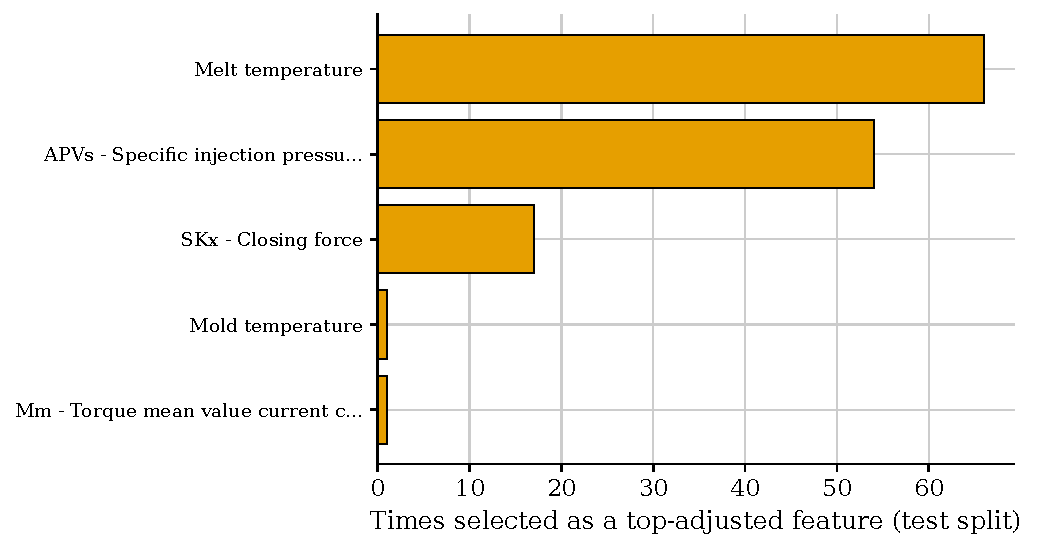
\includegraphics[width=0.85\textwidth]{figures/ch4/fig_ch4_top_adjusted_features.pdf}
\caption{The five process parameters most frequently selected as the top-adjusted feature by the three-tier engine across all resolved test-split cases. Source: \texttt{figures/ch4/fig\_ch4\_top\_adjusted\_features}, \texttt{models/rca\_evaluation\_test.json}.}
\label{fig:ch4-top-adjusted-features}
\end{figure}

\textbf{Table 4.15.} Adjustment frequency of the five most frequently selected parameters, test split. Source: \texttt{models/rca\_evaluation\_test.json} → \texttt{top\_adjusted\_features}.

\begin{longtable}[]{@{}ll@{}}
\toprule\noalign{}
Parameter & Times selected as top-adjusted feature \\
\midrule\noalign{}
\endhead
\bottomrule\noalign{}
\endlastfoot
\emph{{[}Insert rank 1 parameter{]}} & \emph{{[}Insert count{]}} \\
\emph{{[}Insert rank 2 parameter{]}} & \emph{{[}Insert count{]}} \\
\emph{{[}Insert rank 3 parameter{]}} & \emph{{[}Insert count{]}} \\
\emph{{[}Insert rank 4 parameter{]}} & \emph{{[}Insert count{]}} \\
\emph{{[}Insert rank 5 parameter{]}} & \emph{{[}Insert count{]}} \\
\end{longtable}

The distribution is expected to track the global SHAP ranking of §4.3.1, since Tier 1 selects features by local \textbar SHAP\textbar{} and the local rankings aggregate toward the global one. The interpretive question, addressed in §5.1, is whether the parameters the engine most often reaches for are the ones a process engineer would reach for --- the timings that dominate the SHAP ranking, or the temperatures and pressures that dominate conventional molding troubleshooting practice.

Mean sparsity across resolved test-split cases is \textbf{4.88 features} of a possible five (§4.5.3), so the engine is using nearly its full Tier-1 budget on almost every cycle. Recipes with four rather than five adjustments occur where a selected feature's LIME coefficient produced no net movement before acceptance.

\hypertarget{worked-counterfactual-example}{%
\subsection{4.4.4 Worked Counterfactual Example}\label{worked-counterfactual-example}}

Table 4.16 gives a complete worked case: test-split index 39, a cycle with ground-truth label \emph{Waste} that the engine resolved at Tier 1 \textbf{and that the independent verifier confirmed} --- one of the nine confirmed cases on the test split.

\textbf{Table 4.16.} Validator-confirmed worked counterfactual case, test-split index 39, in engineering units. Source: \texttt{thesis\_assets/data/counterfactual\_case\_table.csv}, \texttt{counterfactual\_cases.json}.

\begin{longtable}[]{@{}lllll@{}}
\toprule\noalign{}
Parameter & Original & Suggested & Δ & Direction \\
\midrule\noalign{}
\endhead
\bottomrule\noalign{}
\endlastfoot
SKx -- Closing force (N) & 908.60 & 904.424 & −4.176 & ↓ \\
time\_to\_fill (s) & 6.968 & 6.5562 & −0.4118 & ↓ \\
ZDx -- Plasticizing time (s) & 4.08 & 4.3032 & +0.2232 & ↑ \\
Mold temperature (°C) & 81.402 & 81.139 & −0.263 & ↓ \\
ZUx -- Cycle time (s) & 74.82 & 74.9008 & +0.0808 & ↑ \\
\end{longtable}

\textbf{Model assessment before and after:}

\begin{longtable}[]{@{}
  >{\raggedright\arraybackslash}p{(\columnwidth - 4\tabcolsep) * \real{0.3333}}
  >{\raggedright\arraybackslash}p{(\columnwidth - 4\tabcolsep) * \real{0.3333}}
  >{\raggedright\arraybackslash}p{(\columnwidth - 4\tabcolsep) * \real{0.3333}}@{}}
\toprule\noalign{}
\begin{minipage}[b]{\linewidth}\raggedright
Quantity
\end{minipage} & \begin{minipage}[b]{\linewidth}\raggedright
Original cycle
\end{minipage} & \begin{minipage}[b]{\linewidth}\raggedright
Counterfactual
\end{minipage} \\
\midrule\noalign{}
\endhead
\bottomrule\noalign{}
\endlastfoot
P(Waste) & 0.8366 & 0.1060 \\
P(Acceptable) & 0.1501 & 0.1136 \\
P(Target) & 0.0066 & 0.6293 \\
P(Inefficient) & 0.0066 & 0.1511 \\
\textbf{Conforming confidence P(Acc) + P(Target)} & \textbf{0.1567} & \textbf{0.7429} \\
Independent verifier & --- & \textbf{\checkmark Confirmed} \\
\end{longtable}

The original cycle is classified \emph{Waste} with 83.66\% probability and carries only 15.67\% conforming confidence. The recommended recipe adjusts five parameters and lifts conforming confidence to 74.29\%, with the probability mass moving decisively to \emph{Target} (62.93\%).

Three features of this recipe are worth drawing out, because they illustrate what the engine does well and where the interpretive difficulty in §4.5 originates.

\textbf{The adjustments are small.} The largest change is a 4.18 N reduction in closing force on a base of 908.6 N --- a 0.46\% adjustment. Filling time drops by 0.41 s, plasticizing time rises by 0.22 s, mold temperature falls by a quarter of a degree, and cycle time rises by 0.08 s. Every one of these is within the resolution an operator can actually set on a machine panel, and none requires an excursion from normal operating practice.

\textbf{The adjustments are coherent as a process intervention.} Filling faster while plasticizing longer and holding the mold marginally cooler is a recognisable combination rather than an arbitrary vector, and the near-zero cycle-time change indicates the recipe does not trade quality against throughput.

\textbf{And yet smallness is exactly what makes the result hard to interpret.} A 0.46\% change in closing force moving a cycle from 83.66\% \emph{Waste} to 62.93\% \emph{Target} is a very large change in model output for a very small change in input. The physically plausible reading is that this cycle sits close to a genuine process boundary. The less comfortable reading, and the one §2.7.2 anticipates, is that it sits close to a \emph{model} boundary whose location reflects the training data's particular arrangement rather than the process. From within the model, these two readings are indistinguishable --- which is precisely why the verifier exists, and why §4.5 reports what happens when it is consulted across the whole population rather than on a case selected for having passed.

A second worked case, test index 5, is reported in \texttt{thesis\_assets/data/counterfactual\_cases.json} as the contrasting exhibit: an \emph{Inefficient} cycle that the engine also resolved at Tier 1, reaching 58.01\% conforming confidence, but which the verifier did \textbf{not} confirm. Its recipe is comparably small and comparably coherent, and nothing on the face of it distinguishes it from the confirmed case. That indistinguishability is the finding of the next section.

\begin{center}\rule{0.5\linewidth}{0.5pt}\end{center}

\hypertarget{independent-validation-and-the-circularity-finding}{%
\section{4.5 Independent Validation and the Circularity Finding}\label{independent-validation-and-the-circularity-finding}}

This section reports the central result of the thesis. §4.4 established that the engine resolves 95.24\% of the non-conforming cycles it is given. This section asks what fraction of those resolutions survives a check by a model that played no part in producing them.

\hypertarget{validator-confirmation-rates}{%
\subsection{4.5.1 Validator Confirmation Rates}\label{validator-confirmation-rates}}

\textbf{Table 4.17.} Self-reported resolution against independently confirmed resolution, both splits, default configuration. Source: \texttt{models/rca\_evaluation\_\{val,test\}.json}.

\begin{longtable}[]{@{}
  >{\raggedright\arraybackslash}p{(\columnwidth - 10\tabcolsep) * \real{0.1667}}
  >{\raggedright\arraybackslash}p{(\columnwidth - 10\tabcolsep) * \real{0.1667}}
  >{\raggedright\arraybackslash}p{(\columnwidth - 10\tabcolsep) * \real{0.1667}}
  >{\raggedright\arraybackslash}p{(\columnwidth - 10\tabcolsep) * \real{0.1667}}
  >{\raggedright\arraybackslash}p{(\columnwidth - 10\tabcolsep) * \real{0.1667}}
  >{\raggedright\arraybackslash}p{(\columnwidth - 10\tabcolsep) * \real{0.1667}}@{}}
\toprule\noalign{}
\begin{minipage}[b]{\linewidth}\raggedright
Split
\end{minipage} & \begin{minipage}[b]{\linewidth}\raggedright
N non-conforming
\end{minipage} & \begin{minipage}[b]{\linewidth}\raggedright
Resolved
\end{minipage} & \begin{minipage}[b]{\linewidth}\raggedright
Resolution rate
\end{minipage} & \begin{minipage}[b]{\linewidth}\raggedright
Validator confirmed
\end{minipage} & \begin{minipage}[b]{\linewidth}\raggedright
Validator rate
\end{minipage} \\
\midrule\noalign{}
\endhead
\bottomrule\noalign{}
\endlastfoot
val & 147 & 144 & \textbf{97.96\%} & 16 & \textbf{11.11\%} \\
\textbf{test} & \textbf{147} & \textbf{140} & \textbf{95.24\%} & \textbf{9} & \textbf{6.43\%} \\
\end{longtable}

On the held-out test split, the engine resolves 140 of 147 non-conforming cycles and the independent verifier confirms \textbf{9 of those 140 --- a confirmation rate of 6.43\%.}

The two figures in that sentence describe the same 140 recommendations. The first is what the engine reports about itself; the second is what a model of a different family, trained with a different seed, taking no part in the search, says about the same set of counterfactuals. \textbf{The gap is 88.81 percentage points.}

Stated operationally: at the default configuration, the system issues 140 corrective recommendations to operators, of which 131 carry no independent corroboration.

\textbf{The validation--test difference is itself informative, and the direction matters.} The validation split shows a materially higher confirmation rate (11.11\%) than the test split (6.43\%) --- 16 confirmations of 144 against 9 of 140. The validation split is not a clean estimate: it was used for the model comparison of §4.2.1 and therefore participated in selecting the champion whose decision surface the counterfactual search traverses. Its higher confirmation rate is exactly the optimism that §3.4.4 and Cawley and Talbot {[}84{]} predict from evaluating on data that informed a selection decision. \textbf{The 6.43\% test figure is the one reported as the result}, in accordance with §3.9.5, and the presence of a more favourable number one split away is precisely why that rule exists.

The verifier's own competence is not in question as an explanation. Its training accuracy is reported at initialisation, and the MLP family achieved 0.9218 cross-validation mean accuracy and 0.8931 validation accuracy as a standalone candidate in Table 4.3. A model that classifies real cycles at roughly 90\% accuracy is not failing to recognise conforming parameter vectors in general. It is declining to accept these particular ones.

\hypertarget{characterising-the-gap}{%
\subsection{4.5.2 Characterising the Gap}\label{characterising-the-gap}}

Several explanations for a discrepancy of this size are available, and they are not equally supported.

\textbf{It is not an artefact of the verifier being weak.} As noted above, the MLP classifies genuine cycles competently. If it systematically failed to recognise conforming vectors, it would misclassify the conforming portion of the test split too, and it does not.

\textbf{It is not an artefact of the counterfactuals being unbounded or extreme.} §3.6.5 guarantees that every recommendation lies within the training range of every parameter, enforced by clipping at every iteration. Mean proximity on the test split is 0.5161 in scaled units across a space of width 2 (§4.5.3), so the counterfactuals are close to their originating cycles, not distant excursions.

\textbf{It is not an artefact of the acceptance criterion being trivially permissive.} The criterion requires conforming confidence ≥ 0.55, a margin above bare majority, and the worked case of §4.4.4 reaches 74.29\% --- comfortably clear of the threshold. Yet the great majority of accepted counterfactuals at comparable confidence are rejected by the verifier.

\textbf{The explanation consistent with the evidence is the one §2.7.2 anticipates.} The search terminates at points that satisfy the champion model's decision geometry. Where that geometry reflects a genuine process regularity, a second model trained on the same data should tend to agree, because both are estimating the same underlying relationship. Where it reflects the particular arrangement of the training sample --- the specific placement of axis-aligned splits that a random forest happens to have learned --- a model with a fundamentally different inductive bias has no reason to agree, and mostly does not. Laugel et al.~{[}62{]} describe precisely this as the risk of \emph{unjustified} counterfactuals: points continuously connected to the model's favourable region but not to the data's.

The distribution of nearest-neighbour distances supports this reading. Mean NN distance for the three-tier engine on the test split is \textbf{0.829} in scaled units (§4.5.3) --- that is, the average counterfactual sits 0.829 units away from the nearest real conforming cycle in the training data, in a space where each parameter spans 2 units. The counterfactuals are not landing in the neighbourhoods where conforming production has actually been observed. They are landing in regions the champion model \emph{labels} conforming.

\textbf{What this does not mean.} It does not mean the recommendations are wrong. A counterfactual can be unconfirmed by the verifier and still be a correct process intervention; the verifier is a second learned model, not the machine. The finding bounds what may be claimed from a counterfactual RCA engine's self-report --- it does not establish the truth or falsity of any individual recipe. §5.2.4 develops the resulting position: counterfactual recipes should be presented to operators as \textbf{hypotheses for evaluation}, not as verified corrective actions.

\hypertarget{comparison-against-the-centroid-ablation}{%
\subsection{4.5.3 Comparison Against the Centroid Ablation}\label{comparison-against-the-centroid-ablation}}

A single engine reporting a low confirmation rate is a fact about that engine. The ablation of §3.6.7 tests whether the finding generalises to the method class by removing SHAP feature selection and LIME directional guidance while holding the acceptance criterion, step size, iteration budget, champion model, and verifier constant.

\textbf{Table 4.18.} All five counterfactual metrics for both methods on both splits, with the corresponding McNemar exact-test p-value. Source: \texttt{models/rca\_comparison\_\{val,test\}.json}.

\begin{longtable}[]{@{}
  >{\raggedright\arraybackslash}p{(\columnwidth - 14\tabcolsep) * \real{0.1250}}
  >{\raggedright\arraybackslash}p{(\columnwidth - 14\tabcolsep) * \real{0.1250}}
  >{\raggedright\arraybackslash}p{(\columnwidth - 14\tabcolsep) * \real{0.1250}}
  >{\raggedright\arraybackslash}p{(\columnwidth - 14\tabcolsep) * \real{0.1250}}
  >{\raggedright\arraybackslash}p{(\columnwidth - 14\tabcolsep) * \real{0.1250}}
  >{\raggedright\arraybackslash}p{(\columnwidth - 14\tabcolsep) * \real{0.1250}}
  >{\raggedright\arraybackslash}p{(\columnwidth - 14\tabcolsep) * \real{0.1250}}
  >{\raggedright\arraybackslash}p{(\columnwidth - 14\tabcolsep) * \real{0.1250}}@{}}
\toprule\noalign{}
\begin{minipage}[b]{\linewidth}\raggedright
Split
\end{minipage} & \begin{minipage}[b]{\linewidth}\raggedright
Method
\end{minipage} & \begin{minipage}[b]{\linewidth}\raggedright
Resolution rate
\end{minipage} & \begin{minipage}[b]{\linewidth}\raggedright
Validator rate
\end{minipage} & \begin{minipage}[b]{\linewidth}\raggedright
Mean proximity
\end{minipage} & \begin{minipage}[b]{\linewidth}\raggedright
Mean sparsity
\end{minipage} & \begin{minipage}[b]{\linewidth}\raggedright
Mean NN distance
\end{minipage} & \begin{minipage}[b]{\linewidth}\raggedright
McNemar \emph{p}
\end{minipage} \\
\midrule\noalign{}
\endhead
\bottomrule\noalign{}
\endlastfoot
val & 3-tier RCA & 0.9796 & 0.1111 & 0.5351 & 4.90 & 0.8066 & 0.625 \\
val & Centroid ablation & 0.9796 & 0.1250 & 0.6583 & 12.40 & 0.6805 & 0.625 \\
\textbf{test} & \textbf{3-tier RCA} & \textbf{0.9524} & \textbf{0.0643} & \textbf{0.5161} & \textbf{4.88} & \textbf{0.8290} & \textbf{0.180} \\
\textbf{test} & \textbf{Centroid ablation} & \textbf{0.9524} & \textbf{0.1000} & \textbf{0.6783} & \textbf{12.32} & \textbf{0.6864} & \textbf{0.180} \\
\end{longtable}

\begin{figure}[htbp]
\centering
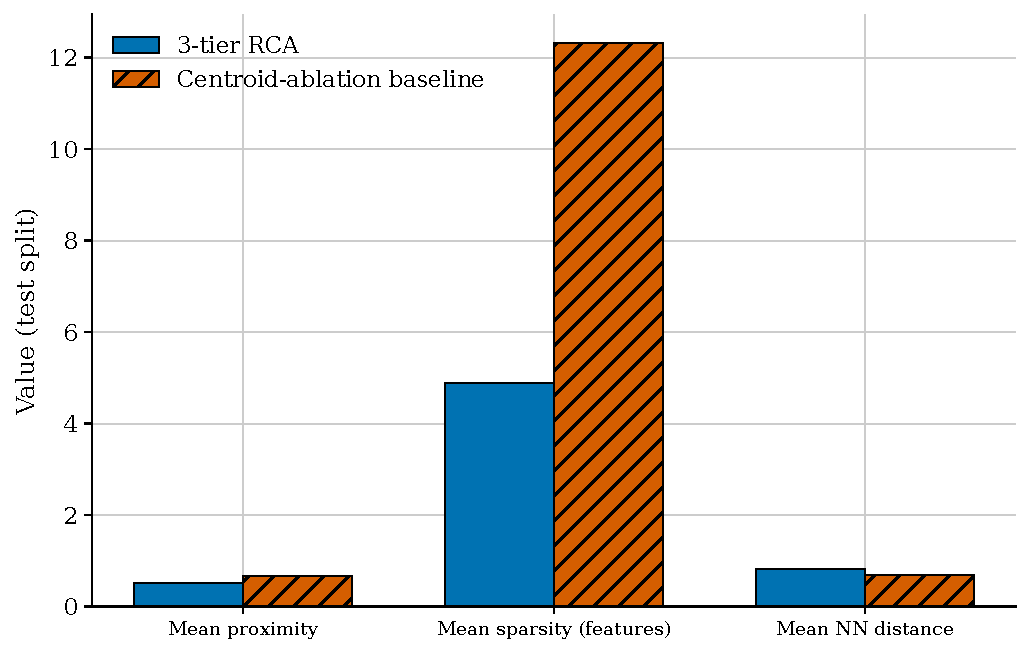
\includegraphics[width=0.85\textwidth]{figures/ch4/fig_ch4_method_comparison_metrics.pdf}
\caption{Mean proximity, sparsity, and nearest-conforming-neighbour distance for the three-tier engine versus the centroid-ablation baseline, test split. Source: \texttt{figures/ch4/fig\_ch4\_method\_comparison\_metrics}.}
\label{fig:ch4-method-comparison-metrics}
\end{figure}

\begin{figure}[htbp]
\centering
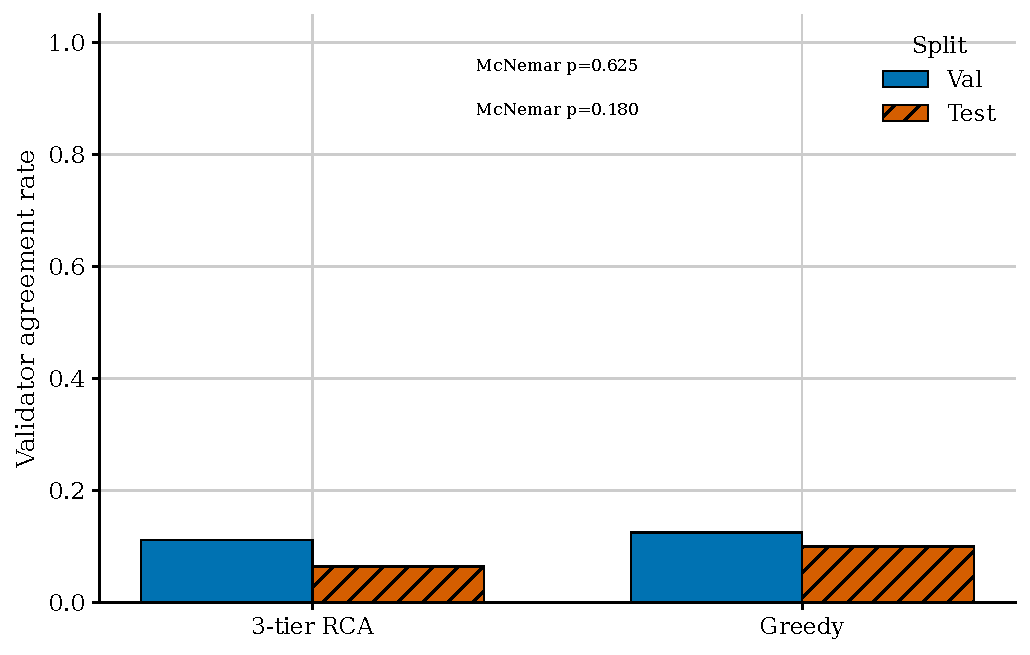
\includegraphics[width=0.85\textwidth]{figures/ch4/fig_ch4_validator_by_split_method.pdf}
\caption{Independent-validator agreement rate for both methods on both splits, with the McNemar exact-test p-value annotated for each split. Source: \texttt{figures/ch4/fig\_ch4\_validator\_by\_split\_method}.}
\label{fig:ch4-validator-by-split-method}
\end{figure}

The first observation is that \textbf{the two methods resolve identically}: 140 of 147 on test, 144 of 147 on validation, for both. This is not a coincidence and is not evidence that the methods are equivalent --- it is a consequence of the matched acceptance criterion and of the fact that the unresolved cases in both are the same seven Tier-0 short-circuits, which depend on the champion model rather than on the search. With resolution held equal by construction, the remaining four metrics isolate the effect of the ablated components cleanly.

The second observation is the important one. \textbf{The centroid ablation achieves a \emph{higher} independent confirmation rate than the three-tier engine} on both splits: 10.00\% against 6.43\% on test (14 confirmations against 9), and 12.50\% against 11.11\% on validation.

This is not the result the engine's design would predict, and it is reported here without softening. The method that removes SHAP feature selection and LIME directional guidance --- the two components that constitute this work's contribution to the search itself --- produces recommendations that an independent model endorses more often. §4.5.4 establishes that the difference is not statistically distinguishable from chance, and §4.5.5 explains why the structure of the two methods makes this outcome unsurprising in retrospect. But the direction of the difference is real and it is not favourable to the proposed engine.

The third observation is that \textbf{both rates are low.} 6.43\% and 10.00\% are both far from anything that would license describing either method's output as verified. Whatever separates the two methods is small relative to what they have in common, and what they have in common is a confirmation rate in the single digits to low tens of percent.

\hypertarget{statistical-significance}{%
\subsection{4.5.4 Statistical Significance}\label{statistical-significance}}

The comparison concerns paired binary outcomes --- each non-conforming cycle is analysed by both methods, and each method's result for that cycle is either confirmed or not --- so McNemar's exact two-sided test was applied per §3.9.4.

\textbf{Table 4.19.} McNemar contingency table, test split, per-sample verifier outcomes for the two methods. Source: \texttt{models/rca\_comparison\_test.json}.

\begin{longtable}[]{@{}llll@{}}
\toprule\noalign{}
& Ablation confirmed & Ablation not confirmed & Row total \\
\midrule\noalign{}
\endhead
\bottomrule\noalign{}
\endlastfoot
\textbf{3-tier confirmed} & 14 & 2 & 16 \\
\textbf{3-tier not confirmed} & 7 & 124 & 131 \\
\textbf{Column total} & 21 & 126 & 147 \\
\end{longtable}

\textbf{McNemar exact test, test split: statistic = 2.0, \emph{p} = 0.1797.} Not significant at α = 0.05.

\textbf{McNemar exact test, validation split: \emph{p} = 0.625.} Not significant at α = 0.05. \emph{{[}Insert the validation contingency table from \texttt{models/rca\_comparison\_val.json} → \texttt{mcnemar\_test.contingency}.{]}}

\textbf{Convention used.} The test operates on the raw per-sample verifier flag. The seven Tier-0 already-conforming cycles carry a positive flag for \textbf{both} methods, because the engine returns \texttt{validator\_ok\ =\ True} for a cycle it declines to modify. They therefore contribute to the concordant ``both confirmed'' cell (14) and do not enter either discordant cell. Since McNemar conditions only on the discordant cells, these seven cases have \textbf{no effect on the statistic or the p-value}. The aggregate confirmation rates of §4.5.1 and Table 4.18, by contrast, are computed over resolved cases only and exclude them --- which is why the row totals here (16 and 21) exceed the confirmed counts reported there (9 and 14) by exactly seven.

The discordant cells are the evidential content: \textbf{7 cycles where only the ablation's recommendation was confirmed, against 2 where only the three-tier engine's was.} With 9 discordant pairs in total, an exact binomial test on a 7:2 split yields \emph{p} = 0.1797. This is a small number of discordant observations, and the test is correspondingly underpowered --- a point returned to in §5.5.

\textbf{Interpretation, stated carefully.} A non-significant McNemar result does not prove the two methods equivalent. Absence of evidence for a difference is not evidence of absence, and at nine discordant pairs the test could not have detected a moderate difference. What the result licenses is the conditional statement prepared in §3.9.4:

\begin{quote}
The independent-confirmation rates of two structurally different counterfactual search strategies are statistically indistinguishable on this data.
\end{quote}

Combined with the ablation framing of §3.6.7 --- the two methods share an acceptance criterion, a champion model, a verifier, a step size, and a search paradigm, and differ in feature selection and directional guidance --- this indistinguishability is \textbf{consistent with the confirmation rate being a property of the shared approach rather than of either implementation}. The three-tier engine's low confirmation rate is not a defect of SHAP-guided search that a better feature-selection scheme would fix, because removing SHAP-guided search entirely does not fix it.

This is the argument by which the finding of §4.5.1 is generalised from one algorithm to a method class. It is an argument from a non-significant test on a small sample, and it is stated at that strength --- as evidence consistent with a claim, not as a demonstration of it.

\hypertarget{where-each-method-wins}{%
\subsection{4.5.5 Where Each Method Wins}\label{where-each-method-wins}}

The two methods differ sharply on three of the five metrics, and the differences are systematic rather than incidental.

\textbf{Table 4.20.} Metric-by-metric comparison, test split, with the structural explanation for each difference.

\begin{longtable}[]{@{}
  >{\raggedright\arraybackslash}p{(\columnwidth - 8\tabcolsep) * \real{0.2000}}
  >{\raggedright\arraybackslash}p{(\columnwidth - 8\tabcolsep) * \real{0.2000}}
  >{\raggedright\arraybackslash}p{(\columnwidth - 8\tabcolsep) * \real{0.2000}}
  >{\raggedright\arraybackslash}p{(\columnwidth - 8\tabcolsep) * \real{0.2000}}
  >{\raggedright\arraybackslash}p{(\columnwidth - 8\tabcolsep) * \real{0.2000}}@{}}
\toprule\noalign{}
\begin{minipage}[b]{\linewidth}\raggedright
Metric
\end{minipage} & \begin{minipage}[b]{\linewidth}\raggedright
3-tier
\end{minipage} & \begin{minipage}[b]{\linewidth}\raggedright
Ablation
\end{minipage} & \begin{minipage}[b]{\linewidth}\raggedright
Winner
\end{minipage} & \begin{minipage}[b]{\linewidth}\raggedright
Explanation
\end{minipage} \\
\midrule\noalign{}
\endhead
\bottomrule\noalign{}
\endlastfoot
Resolution rate & 0.9524 & 0.9524 & Tie & Matched acceptance criterion; identical Tier-0 exclusions \\
Mean sparsity & \textbf{4.88} & 12.32 & \textbf{3-tier} & Tier 1 adjusts 5 SHAP-selected features; ablation adjusts all 13 \\
Mean proximity & \textbf{0.5161} & 0.6783 & \textbf{3-tier} & Fewer moving parameters means shorter total displacement \\
Mean NN distance & 0.8290 & \textbf{0.6864} & \textbf{Ablation} & Ablation moves explicitly toward the conforming centroid \\
Validator rate & 0.0643 & \textbf{0.1000} & \textbf{Ablation} & --- \\
\end{longtable}

\textbf{The three-tier engine wins decisively on actionability.} Its recipes touch a mean of \textbf{4.88 parameters against the ablation's 12.32} --- a 2.5-fold difference --- and are \textbf{24\% closer} to the originating cycle in scaled space (0.5161 against 0.6783). Both differences are large relative to the metrics' scales and both were anticipated in §3.6.7 as direct consequences of the designs. A recipe of five adjustments is something an operator can execute and reason about; a recipe of twelve is a wholesale reconfiguration of the machine, and one whose individual components an operator cannot separately assess. If the question is which method produces a usable work instruction, the answer is unambiguous.

\textbf{The ablation wins on nearest-neighbour distance (0.6864 against 0.8290), and this metric structurally favours it.} This was stated in advance in §3.6.7 and is restated here so that the result is not over-read. The ablation's entire search consists of moving toward the centroid of conforming training samples. A metric that measures distance to the nearest conforming training sample is therefore measuring, in part, how directly a method aims at the region that metric rewards. Reporting the ablation as ``more plausible'' on this basis would be close to circular. The honest statement is that the ablation terminates closer to observed conforming production, by construction, and that the three-tier engine's counterfactuals sit further from it.

\textbf{The ablation also wins on validator rate, and this is not structurally explained away.} The nearest-neighbour result and the confirmation result point the same way: the method that ends closer to real conforming cycles is also the method a second model more often endorses. That is a coherent story, and it is unfavourable to the proposed engine. §5.2 takes it up.

The overall picture is a clean instance of the desiderata conflict established in §2.4.4 and the reason §3.9.2 requires reporting all five metrics rather than a favourable subset. \textbf{No configuration wins on everything.} The three-tier engine produces recommendations that are sparse, proximate, and actionable --- and less often independently corroborated. The ablation produces recommendations that are dense, distant from the original cycle, and closer to observed conforming production --- and slightly more often corroborated. A study reporting only sparsity and proximity would conclude the three-tier engine is better. A study reporting only nearest-neighbour distance and validator rate would conclude the ablation is. Both conclusions would be selective reporting of the same experiment.

\begin{center}\rule{0.5\linewidth}{0.5pt}\end{center}

\hypertarget{tier-cascade-sensitivity}{%
\section{4.6 Tier Cascade Sensitivity}\label{tier-cascade-sensitivity}}

§4.5 established a gap between self-reported and independently confirmed resolution at the default operating point. This section asks whether that gap is a fixed property of the engine or a function of how it is configured. The answer is the second, and it is the most practically consequential result in the chapter.

Two sweeps were run on both splits: the \textbf{acceptance threshold} across \{0.55, 0.65, 0.75, 0.85, 0.95\} with the iteration budget fixed at 150, and the \textbf{iteration budget} across \{10, 25, 50, 150\} with the threshold fixed at 0.55.

\hypertarget{threshold-sweep}{%
\subsection{4.6.1 Threshold Sweep}\label{threshold-sweep}}

\textbf{Table 4.21.} Acceptance-threshold sweep, test split (n = 147 non-conforming cycles per configuration), iteration budget fixed at 150. Source: \texttt{models/tier\_sensitivity\_test.json}.

\begin{longtable}[]{@{}
  >{\raggedright\arraybackslash}p{(\columnwidth - 16\tabcolsep) * \real{0.1111}}
  >{\raggedright\arraybackslash}p{(\columnwidth - 16\tabcolsep) * \real{0.1111}}
  >{\raggedright\arraybackslash}p{(\columnwidth - 16\tabcolsep) * \real{0.1111}}
  >{\raggedright\arraybackslash}p{(\columnwidth - 16\tabcolsep) * \real{0.1111}}
  >{\raggedright\arraybackslash}p{(\columnwidth - 16\tabcolsep) * \real{0.1111}}
  >{\raggedright\arraybackslash}p{(\columnwidth - 16\tabcolsep) * \real{0.1111}}
  >{\raggedright\arraybackslash}p{(\columnwidth - 16\tabcolsep) * \real{0.1111}}
  >{\raggedright\arraybackslash}p{(\columnwidth - 16\tabcolsep) * \real{0.1111}}
  >{\raggedright\arraybackslash}p{(\columnwidth - 16\tabcolsep) * \real{0.1111}}@{}}
\toprule\noalign{}
\begin{minipage}[b]{\linewidth}\raggedright
Threshold
\end{minipage} & \begin{minipage}[b]{\linewidth}\raggedright
Tier 1
\end{minipage} & \begin{minipage}[b]{\linewidth}\raggedright
Tier 2
\end{minipage} & \begin{minipage}[b]{\linewidth}\raggedright
Tier 3
\end{minipage} & \begin{minipage}[b]{\linewidth}\raggedright
Resolved
\end{minipage} & \begin{minipage}[b]{\linewidth}\raggedright
Resolution rate
\end{minipage} & \begin{minipage}[b]{\linewidth}\raggedright
Confirmed
\end{minipage} & \begin{minipage}[b]{\linewidth}\raggedright
Validator rate
\end{minipage} & \begin{minipage}[b]{\linewidth}\raggedright
Runtime (s)
\end{minipage} \\
\midrule\noalign{}
\endhead
\bottomrule\noalign{}
\endlastfoot
\textbf{0.55} (default) & 140 & 0 & 0 & 140 & \textbf{95.24\%} & 9 & \textbf{6.43\%} & 71 \\
0.65 & 140 & 0 & 2 & 140 & 95.24\% & 13 & 9.29\% & 143 \\
0.75 & 89 & 21 & 33 & 110 & 74.83\% & 24 & 21.82\% & 477 \\
0.85 & 21 & 24 & 98 & 45 & 30.61\% & 20 & 44.44\% & 904 \\
0.95 & 1 & 6 & 137 & 7 & \textbf{4.76\%} & 6 & \textbf{85.71\%} & 1,084 \\
\end{longtable}

\textbf{Table 4.22.} Acceptance-threshold sweep, validation split (n = 147), iteration budget fixed at 150. Source: \texttt{models/tier\_sensitivity\_val.json}.

\begin{longtable}[]{@{}
  >{\raggedright\arraybackslash}p{(\columnwidth - 16\tabcolsep) * \real{0.1111}}
  >{\raggedright\arraybackslash}p{(\columnwidth - 16\tabcolsep) * \real{0.1111}}
  >{\raggedright\arraybackslash}p{(\columnwidth - 16\tabcolsep) * \real{0.1111}}
  >{\raggedright\arraybackslash}p{(\columnwidth - 16\tabcolsep) * \real{0.1111}}
  >{\raggedright\arraybackslash}p{(\columnwidth - 16\tabcolsep) * \real{0.1111}}
  >{\raggedright\arraybackslash}p{(\columnwidth - 16\tabcolsep) * \real{0.1111}}
  >{\raggedright\arraybackslash}p{(\columnwidth - 16\tabcolsep) * \real{0.1111}}
  >{\raggedright\arraybackslash}p{(\columnwidth - 16\tabcolsep) * \real{0.1111}}
  >{\raggedright\arraybackslash}p{(\columnwidth - 16\tabcolsep) * \real{0.1111}}@{}}
\toprule\noalign{}
\begin{minipage}[b]{\linewidth}\raggedright
Threshold
\end{minipage} & \begin{minipage}[b]{\linewidth}\raggedright
Tier 1
\end{minipage} & \begin{minipage}[b]{\linewidth}\raggedright
Tier 2
\end{minipage} & \begin{minipage}[b]{\linewidth}\raggedright
Tier 3
\end{minipage} & \begin{minipage}[b]{\linewidth}\raggedright
Resolved
\end{minipage} & \begin{minipage}[b]{\linewidth}\raggedright
Resolution rate
\end{minipage} & \begin{minipage}[b]{\linewidth}\raggedright
Confirmed
\end{minipage} & \begin{minipage}[b]{\linewidth}\raggedright
Validator rate
\end{minipage} & \begin{minipage}[b]{\linewidth}\raggedright
Runtime (s)
\end{minipage} \\
\midrule\noalign{}
\endhead
\bottomrule\noalign{}
\endlastfoot
0.55 (default) & 144 & 0 & 0 & 144 & 97.96\% & 16 & 11.11\% & 73 \\
0.65 & 142 & 1 & 2 & 143 & 97.28\% & 15 & 10.49\% & 159 \\
0.75 & 99 & 13 & 33 & 112 & 76.19\% & 25 & 22.32\% & 463 \\
0.85 & 25 & 18 & 102 & 43 & 29.25\% & 24 & 55.81\% & 945 \\
0.95 & 0 & 4 & 142 & 4 & 2.72\% & 4 & \textbf{100.00\%} & 1,448 \\
\end{longtable}

\begin{figure}[htbp]
\centering
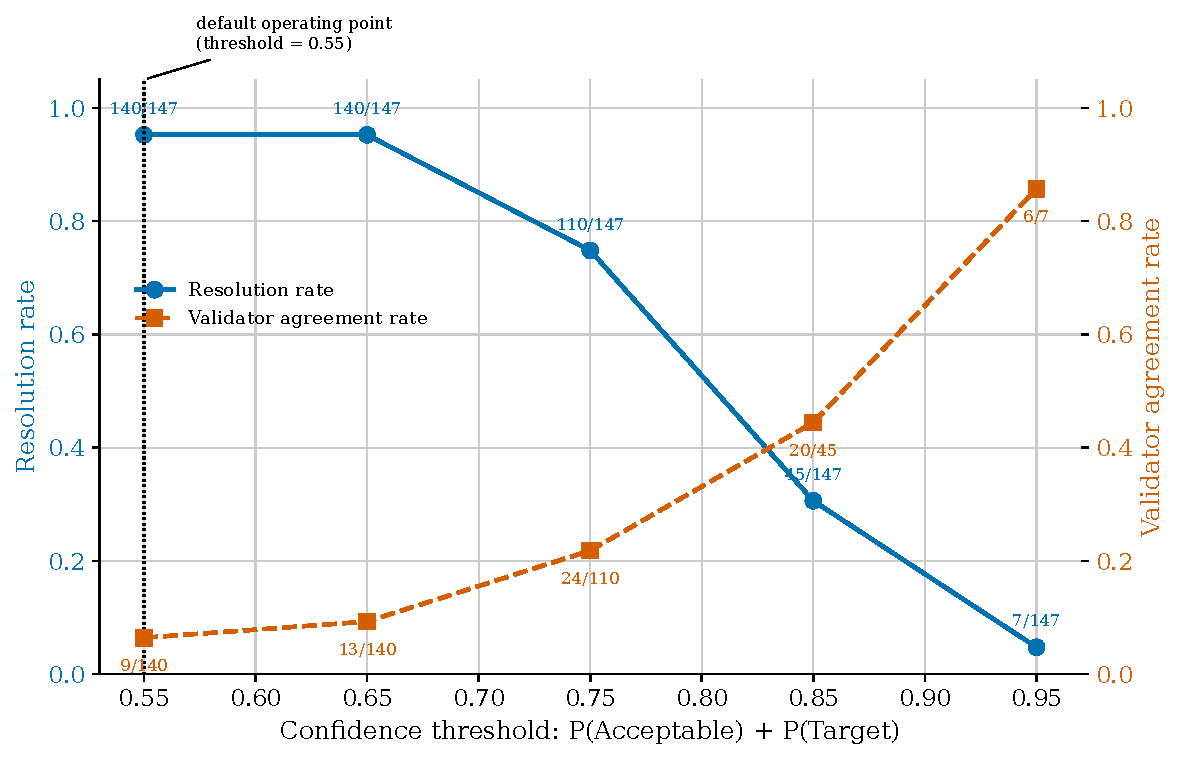
\includegraphics[width=0.85\textwidth]{figures/ch4/fig_ch4_tradeoff_resolution_validator.pdf}
\caption{\textbf{Central result figure.} Resolution rate (falling) and independent-validator agreement rate (rising) as functions of the acceptance-confidence threshold, test split, with the default operating point annotated and raw counts labelled at every marker. Source: \texttt{figures/ch4/fig\_ch4\_tradeoff\_resolution\_validator}.}
\label{fig:ch4-tradeoff-resolution-validator}
\end{figure}

\begin{figure}[htbp]
\centering
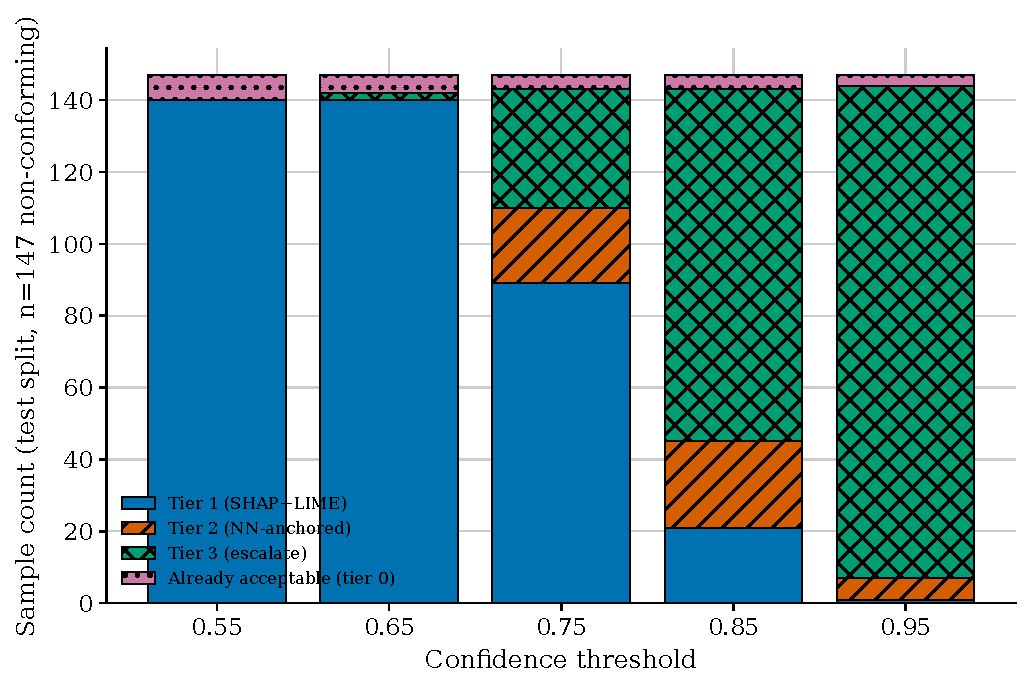
\includegraphics[width=0.85\textwidth]{figures/ch4/fig_ch4_tier_distribution.pdf}
\caption{Distribution of RCA outcomes (Tier 1, Tier 2, Tier 3, already-acceptable) across the five swept thresholds, test split. Source: \texttt{figures/ch4/fig\_ch4\_tier\_distribution}.}
\label{fig:ch4-tier-distribution}
\end{figure}

Three findings.

\textbf{Finding 1 --- The gap is tunable, and the trade-off is near-monotonic.} As the acceptance threshold rises from 0.55 to 0.95 on the test split, resolution rate falls from 95.24\% to 4.76\% while validator agreement rises from 6.43\% to 85.71\%. The validation split shows the same relationship, reaching 100\% agreement at threshold 0.95. Every increment of the threshold buys independent corroboration and pays for it in coverage.

This transforms the finding of §4.5.1 from a defect into an \textbf{operating characteristic}. The 6.43\% confirmation rate is not a fixed property of counterfactual RCA on this dataset; it is the confirmation rate at the most permissive point of a configurable envelope. A deployment can choose where on that curve to sit, and the choice is a genuine engineering decision about the relative cost of an uncorroborated recommendation and a declined one.

The counts at the tight end are small and must be read as such. At threshold 0.95 on test, 6 confirmations of 7 resolutions is 85.71\% with a very wide confidence interval; on validation, 4 of 4 is 100\% on four observations. The \emph{direction} of the relationship is supported across ten configurations and two splits; the precise values at the extremes are not.

\textbf{Finding 2 --- The tier cascade is an active operating envelope.} Tier 2 first activates at threshold 0.65 on validation (1 case) and 0.75 on test (21 cases), reaching 24 cases at threshold 0.85 on test. Tier 3 activates at 0.65 on both splits and becomes dominant above 0.75, accounting for 98 of 147 cycles at 0.85 and 137 of 147 at 0.95 on test.

This settles the question left open in §3.6.4. The tiers are not dormant fallbacks that this dataset never exercises; they are the mechanism by which the cascade responds to a stricter acceptance criterion. As the threshold rises, Tier 1's explanation-guided local search increasingly fails to reach an accepted point, control passes to the nearest-neighbour anchor, and where that also fails the engine escalates. The behaviour is exactly what the design intends, and it is only invisible at the default configuration because the default is permissive.

\textbf{Finding 3 --- Escalation is the engine behaving correctly, not failing.} At threshold 0.95, the engine declines to answer for 137 of 147 cycles. Read against §3.6.4, this is the safety property working: under a demand for high-confidence correction, the engine mostly reports that no parameter adjustment within physical bounds achieves it, and directs the cycle to manual inspection. The 6 of 7 it does answer are answered with recommendations an independent model overwhelmingly endorses.

There is also a computational cost to the strict end: runtime rises from 71 s to 1,084 s on test, a factor of 15, because failed Tier-1 searches run their full iteration budget before Tier 2 begins.

\hypertarget{iteration-budget-sweep}{%
\subsection{4.6.2 Iteration-Budget Sweep}\label{iteration-budget-sweep}}

\textbf{Table 4.23.} Iteration-budget sweep, threshold fixed at 0.55, both splits. Source: \texttt{models/tier\_sensitivity\_\{val,test\}.json}.

\begin{longtable}[]{@{}
  >{\raggedright\arraybackslash}p{(\columnwidth - 14\tabcolsep) * \real{0.1250}}
  >{\raggedright\arraybackslash}p{(\columnwidth - 14\tabcolsep) * \real{0.1250}}
  >{\raggedright\arraybackslash}p{(\columnwidth - 14\tabcolsep) * \real{0.1250}}
  >{\raggedright\arraybackslash}p{(\columnwidth - 14\tabcolsep) * \real{0.1250}}
  >{\raggedright\arraybackslash}p{(\columnwidth - 14\tabcolsep) * \real{0.1250}}
  >{\raggedright\arraybackslash}p{(\columnwidth - 14\tabcolsep) * \real{0.1250}}
  >{\raggedright\arraybackslash}p{(\columnwidth - 14\tabcolsep) * \real{0.1250}}
  >{\raggedright\arraybackslash}p{(\columnwidth - 14\tabcolsep) * \real{0.1250}}@{}}
\toprule\noalign{}
\begin{minipage}[b]{\linewidth}\raggedright
Split
\end{minipage} & \begin{minipage}[b]{\linewidth}\raggedright
Max iter
\end{minipage} & \begin{minipage}[b]{\linewidth}\raggedright
Tier 1
\end{minipage} & \begin{minipage}[b]{\linewidth}\raggedright
Tier 2
\end{minipage} & \begin{minipage}[b]{\linewidth}\raggedright
Tier 3
\end{minipage} & \begin{minipage}[b]{\linewidth}\raggedright
Resolution rate
\end{minipage} & \begin{minipage}[b]{\linewidth}\raggedright
Confirmed
\end{minipage} & \begin{minipage}[b]{\linewidth}\raggedright
Validator rate
\end{minipage} \\
\midrule\noalign{}
\endhead
\bottomrule\noalign{}
\endlastfoot
test & 10 & 83 & 7 & 50 & 61.22\% & 12 & \textbf{13.33\%} \\
test & 25 & 139 & 1 & 0 & 95.24\% & 10 & 7.14\% \\
test & 50 & 140 & 0 & 0 & 95.24\% & 9 & 6.43\% \\
test & 150 & 140 & 0 & 0 & 95.24\% & 9 & 6.43\% \\
val & 10 & 76 & 5 & 63 & 55.10\% & 18 & \textbf{22.22\%} \\
val & 25 & 140 & 3 & 1 & 97.28\% & 19 & 13.29\% \\
val & 50 & 144 & 0 & 0 & 97.96\% & 16 & 11.11\% \\
val & 150 & 144 & 0 & 0 & 97.96\% & 16 & 11.11\% \\
\end{longtable}

\begin{figure}[htbp]
\centering
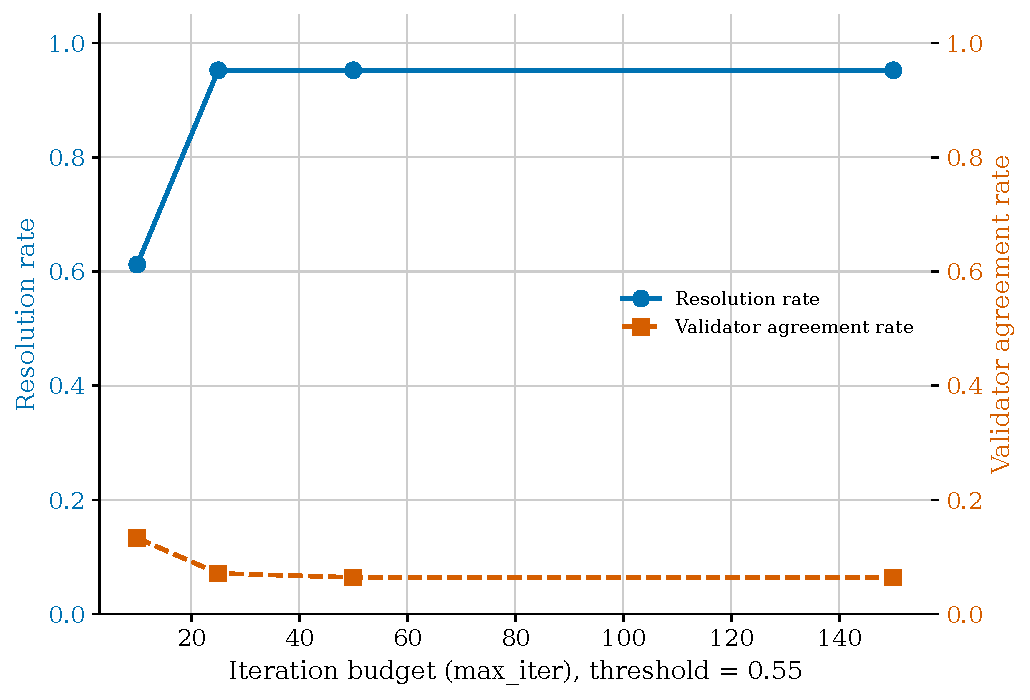
\includegraphics[width=0.85\textwidth]{figures/ch4/fig_ch4_tradeoff_maxiter.pdf}
\caption{Resolution rate and validator agreement as functions of the iteration budget, threshold fixed at 0.55, test split. Source: \texttt{figures/ch4/fig\_ch4\_tradeoff\_maxiter}.}
\label{fig:ch4-tradeoff-maxiter}
\end{figure}

The iteration budget produces the same trade-off through a different mechanism, and the result is arguably more interesting than the threshold sweep because it is less expected.

\textbf{A shorter search yields better-corroborated recommendations.} At an iteration budget of 10 on the test split, resolution falls to 61.22\% but validator agreement rises to 13.33\% --- more than double the default figure --- and on validation to 22.22\%, also roughly double. Restricting how far the search may travel improves the independent quality of what it finds.

The mechanism is the one §2.4.4 and §2.7.2 describe. A counterfactual reached in ten steps of 0.02 lies at most 0.2 scaled units from the original cycle in any parameter. A counterfactual permitted 150 steps may travel up to 3.0 units and saturate at the bounds. The further the search travels from the observed cycle, the more it relies on the model's extrapolation and the less likely a second model is to agree. \textbf{Search effort and independent trustworthiness are inversely related} on this dataset.

\textbf{Saturation occurs by 50 iterations.} The results at 50 and 150 are identical on both splits --- same tier counts, same resolution, same confirmations. The additional 100 iterations change nothing, because every search that succeeds does so within 50 steps and every search that fails would fail at any budget. The default budget of 150 is therefore three times larger than necessary at this threshold, and reducing it to 50 would cut runtime with no effect on results. §5.3 takes up whether it should be reduced further, to a regime where the trade-off is actively used.

\hypertarget{implications-for-the-operating-point}{%
\subsection{4.6.3 Implications for the Operating Point}\label{implications-for-the-operating-point}}

Taken together, the two sweeps show that the engine has a \textbf{two-dimensional operating envelope} and that the default configuration sits at the permissive corner of it: the lowest threshold and an iteration budget three times past saturation. That corner maximises coverage and minimises independent corroboration.

Nothing in this chapter establishes which point on the envelope a deployment should choose, because that depends on the relative cost of a wrong recommendation and a declined one in a particular plant --- a question this thesis has no data to answer. What the sweeps establish is that \textbf{the choice exists, is continuous, and is measurable}, and that reporting a single operating point without characterising the envelope around it would have concealed most of what the engine actually does. §5.3 discusses candidate operating points and the information a plant would need to select among them.

\begin{center}\rule{0.5\linewidth}{0.5pt}\end{center}

\hypertarget{drift-detection-validation}{%
\section{4.7 Drift Detection Validation}\label{drift-detection-validation}}

Per §3.7.3, the reference and current windows both derive from the same stratified split of the same dataset, so no genuine temporal drift is present and none is reported. What is reported is \textbf{detector sensitivity to controlled synthetic perturbation}, which is the claim the available data supports.

For each of the 13 parameters and each shift magnitude k $\in$ \{0, 1, 2, 3\}, the validation set was copied, the selected parameter shifted by k × σ\_train and clipped to the scaled bounds, and PSI recomputed against the training reference.

\textbf{Table 4.24.} PSI response to synthetic distribution shift, selected parameters. Full table for all 13 parameters at all four magnitudes in Appendix D. Thresholds: PSI \textless{} 0.10 stable, 0.10--0.20 moderate, \textgreater{} 0.20 critical. Source: \texttt{models/drift\_validation.json}.

\begin{longtable}[]{@{}
  >{\raggedright\arraybackslash}p{(\columnwidth - 10\tabcolsep) * \real{0.1667}}
  >{\raggedright\arraybackslash}p{(\columnwidth - 10\tabcolsep) * \real{0.1667}}
  >{\raggedright\arraybackslash}p{(\columnwidth - 10\tabcolsep) * \real{0.1667}}
  >{\raggedright\arraybackslash}p{(\columnwidth - 10\tabcolsep) * \real{0.1667}}
  >{\raggedright\arraybackslash}p{(\columnwidth - 10\tabcolsep) * \real{0.1667}}
  >{\raggedright\arraybackslash}p{(\columnwidth - 10\tabcolsep) * \real{0.1667}}@{}}
\toprule\noalign{}
\begin{minipage}[b]{\linewidth}\raggedright
Parameter
\end{minipage} & \begin{minipage}[b]{\linewidth}\raggedright
σ\_train
\end{minipage} & \begin{minipage}[b]{\linewidth}\raggedright
PSI at k = 0
\end{minipage} & \begin{minipage}[b]{\linewidth}\raggedright
PSI at k = 1
\end{minipage} & \begin{minipage}[b]{\linewidth}\raggedright
PSI at k = 2
\end{minipage} & \begin{minipage}[b]{\linewidth}\raggedright
PSI at k = 3
\end{minipage} \\
\midrule\noalign{}
\endhead
\bottomrule\noalign{}
\endlastfoot
Melt temperature & 0.1705 & 0.0259 & 8.2883 & 8.2883 & 8.2883 \\
Mold temperature & 0.2559 & 0.0406 & 2.1087 & 5.1307 & 6.8035 \\
time\_to\_fill & 0.6478 & 0.0195 & 7.6032 & 7.5715 & 7.6140 \\
ZDx -- Plasticizing time & 0.2353 & 0.0512 & 2.9142 & 7.6622 & 8.2924 \\
ZUx -- Cycle time & 0.8592 & 0.0362 & 6.0487 & 5.7814 & 8.1222 \\
SKx -- Closing force & 0.4291 & 0.0573 & 1.5497 & 4.2614 & 7.3632 \\
SKs -- Clamping force peak & 0.4200 & 0.0133 & 2.9266 & 3.9492 & \emph{{[}see artefact{]}} \\
APVs -- Spec. inj. pressure peak & 0.3592 & 0.0257 & 1.9440 & 4.2252 & 4.8287 \\
CPn -- Screw position & 0.3198 & 0.0321 & 1.4790 & 3.7901 & 4.8616 \\
SVo -- Shot volume & 0.3090 & 0.0183 & 1.6420 & 4.8940 & 7.1315 \\
\end{longtable}

\begin{figure}[htbp]
\centering
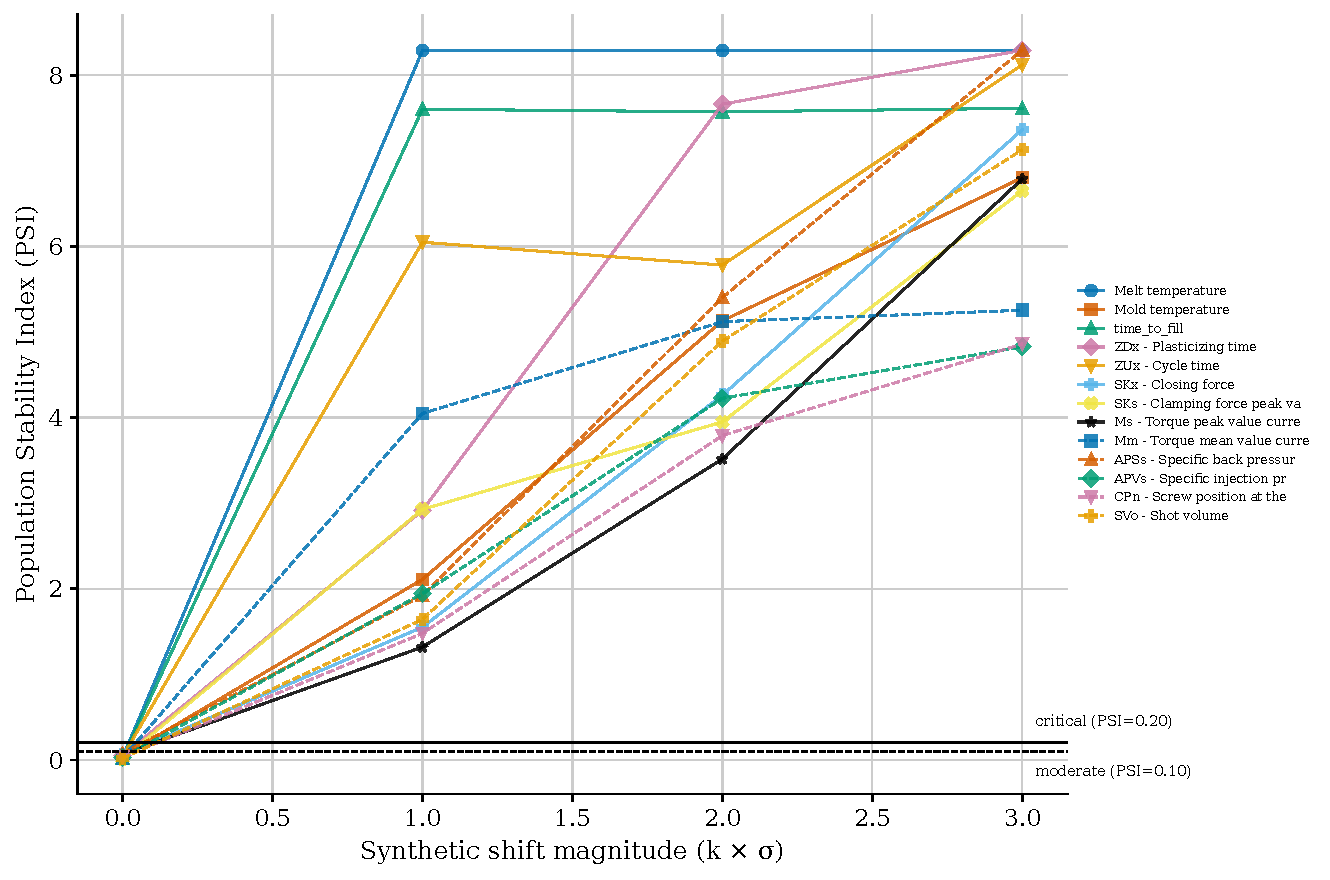
\includegraphics[width=0.85\textwidth]{figures/ch4/fig_ch4_psi_sensitivity.pdf}
\caption{PSI for each of the 13 parameters under synthetic shifts of magnitude k·σ, with the moderate (0.10) and critical (0.20) thresholds marked. Source: \texttt{figures/ch4/fig\_ch4\_psi\_sensitivity}.}
\label{fig:ch4-psi-sensitivity}
\end{figure}

Three results.

\textbf{At k = 0, every parameter is classified stable.} PSI values range from 0.0133 to 0.0573, all below the 0.10 moderate threshold. This is the anticipated baseline stated in §3.7.3: two samples drawn from the same stratified split of the same dataset should look alike, and they do. The non-zero values reflect finite-sample binning variation between 870 training and 290 validation observations, not drift.

\textbf{At k = 1σ, all 13 parameters cross the critical threshold.} The smallest PSI at k = 1 is 1.479 (screw position), more than seven times the 0.20 critical threshold; the largest is 8.288 (melt temperature). \textbf{The detector's trigger magnitude is therefore k = 1σ for all 13 parameters}, with a very wide margin. A one-standard-deviation shift in any single process parameter is detected unambiguously.

\textbf{PSI does not increase monotonically with k for every parameter, and the reason is instructive.} Melt temperature returns exactly 8.2883 at k = 1, 2 and 3; time\_to\_fill returns 7.6032, 7.5715 and 7.6140; cycle time falls from 6.0487 at k = 1 to 5.7814 at k = 2 before rising to 8.1222 at k = 3. This is a consequence of the clipping applied after the shift. Once a shift is large enough to push most of a parameter's mass against the scaled upper bound of +1, further shifting cannot move it, and the resulting distribution --- and its PSI --- saturates. Melt temperature has the smallest σ\_train (0.1705) and saturates first and completely.

The correct conclusion is that \textbf{PSI magnitude beyond the trigger point is not a reliable measure of drift severity in this bounded space}, and PSI should be read as a detector rather than as a magnitude estimator. That is consistent with its conventional use and with the threshold-based interpretation of §3.7.3, but it is worth stating because a reader looking at Table 4.24 might otherwise expect the values to order the severity of the injected shifts, and they do not.

\textbf{Limitations restated.} This is a synthetic sensitivity study, labelled as such throughout. It establishes that the detector responds to controlled single-parameter shifts of known magnitude. It does not establish that the detector would catch the drift patterns a real machine produces, which are typically gradual, multi-parameter, and correlated rather than sudden, univariate, and independent. Real drift monitoring requires temporally separated production data, which this work does not have. The Page-Hinkley detector on the confidence stream was exercised on the validation split and is reported in the application interface, but for the same reason it detects nothing on data with no temporal structure, and no result from it is claimed here.

\begin{center}\rule{0.5\linewidth}{0.5pt}\end{center}

\hypertarget{expert-evaluation-sub-study}{%
\section{4.8 Expert Evaluation Sub-Study}\label{expert-evaluation-sub-study}}

\emph{{[}This section is a placeholder pending collection of expert responses. The instrument is complete and reproduced in Appendix C. If responses are not collected before submission, this section should be removed and the sub-study described in §6.4 as planned work --- a study that was designed but not run must not be reported as though it were run.{]}}

\hypertarget{participants-and-procedure}{%
\subsection{4.8.1 Participants and Procedure}\label{participants-and-procedure}}

\emph{{[}Insert: number of participants; role distribution (process engineer, quality manager, machine operator, academic); experience bands; recruitment route; whether the instrument was administered in person or remotely; date range of collection; language of administration and whether translation was required.{]}}

\emph{{[}Insert consent statement: participation voluntary and informed; responses recorded without identifying information beyond coarse role and experience band; results reported in aggregate only.{]}}

\hypertarget{instrument-design}{%
\subsection{4.8.2 Instrument Design}\label{instrument-design}}

The questionnaire presents each participant with RCA cases drawn from the held-out test split, including at least one verifier-confirmed case (test index 39, reproduced in Table 4.16) and at least one unconfirmed case (test index 5). For each case, participants see the cycle's 13 parameters in engineering units, the model's classification and confidence, the SHAP and LIME explanation, and the recommended adjustments --- \textbf{without} being told the verifier's verdict, so that judgements are not anchored by it.

Four five-point Likert constructs are assessed:

\begin{longtable}[]{@{}
  >{\raggedright\arraybackslash}p{(\columnwidth - 2\tabcolsep) * \real{0.5000}}
  >{\raggedright\arraybackslash}p{(\columnwidth - 2\tabcolsep) * \real{0.5000}}@{}}
\toprule\noalign{}
\begin{minipage}[b]{\linewidth}\raggedright
Construct
\end{minipage} & \begin{minipage}[b]{\linewidth}\raggedright
Item
\end{minipage} \\
\midrule\noalign{}
\endhead
\bottomrule\noalign{}
\endlastfoot
C1 --- Explanation clarity & The explanation makes it clear which process parameters drove this classification. \\
C2 --- Recommendation plausibility & The recommended adjustments are plausible as a process intervention. \\
C3 --- Behavioural intention & I would act on this recommendation on a running machine. \\
C4 --- System trust & I would trust a system of this kind as a decision-support tool in quality control. \\
\end{longtable}

Each item is followed by a free-text field for reasoning. The full instrument, including the case presentations and the demographic items, is reproduced in Appendix C.

\hypertarget{results}{%
\subsection{4.8.3 Results}\label{results}}

\emph{{[}Insert: per-construct mean, median, and distribution across participants; comparison of ratings between the confirmed and unconfirmed cases --- the analytically central comparison, since it tests whether expert judgement distinguishes the cases the independent verifier distinguishes; representative free-text responses, translated where necessary.{]}}

\emph{{[}Table 4.25 placeholder: Likert response distribution by construct.{]}}

\emph{{[}Figure 4.16 placeholder: diverging stacked bar chart of Likert responses by construct.{]}}

\hypertarget{threats-to-validity-given-sample-size}{%
\subsection{4.8.4 Threats to Validity Given Sample Size}\label{threats-to-validity-given-sample-size}}

\emph{{[}Insert once n is known.{]}} The sub-study is \textbf{descriptive rather than inferential} and no significance testing is performed on its results, for the reasons given in §3.9.6: the expert pool available in the local industrial context is small, and inferential statistics on a handful of respondents would convey a precision the design cannot support.

Three threats apply regardless of the realised sample size and are stated here so that the section is not read as stronger than it is.

\textbf{Construct mismatch.} Expert plausibility judgement and recommendation correctness are different constructs. An expert may find a recommendation plausible and be wrong; a correct recommendation may be counter-intuitive. The sub-study measures whether the system's outputs are \emph{credible to domain experts}, which is a necessary condition for adoption and not a sufficient condition for correctness. It complements the independent-validation protocol of §4.5 and does not substitute for it.

\textbf{Selection.} Participants recruited through professional contacts are not a random sample of the population of process engineers, and may be more favourably disposed toward digital quality tools than the population a deployment would encounter.

\textbf{Presentation.} Judgements are made from a static case presentation rather than from use of the running system, so the results speak to the intelligibility of the output rather than to the usability of the application.

\begin{center}\rule{0.5\linewidth}{0.5pt}\end{center}

\hypertarget{summary-of-findings}{%
\section{4.9 Summary of Findings}\label{summary-of-findings}}

\textbf{Table 4.26.} Research questions mapped to results and supporting artefacts. All headline figures are test-split unless stated.

\begin{longtable}[]{@{}
  >{\raggedright\arraybackslash}p{(\columnwidth - 6\tabcolsep) * \real{0.2500}}
  >{\raggedright\arraybackslash}p{(\columnwidth - 6\tabcolsep) * \real{0.2500}}
  >{\raggedright\arraybackslash}p{(\columnwidth - 6\tabcolsep) * \real{0.2500}}
  >{\raggedright\arraybackslash}p{(\columnwidth - 6\tabcolsep) * \real{0.2500}}@{}}
\toprule\noalign{}
\begin{minipage}[b]{\linewidth}\raggedright
RQ
\end{minipage} & \begin{minipage}[b]{\linewidth}\raggedright
Question
\end{minipage} & \begin{minipage}[b]{\linewidth}\raggedright
Result
\end{minipage} & \begin{minipage}[b]{\linewidth}\raggedright
Supporting artefact
\end{minipage} \\
\midrule\noalign{}
\endhead
\bottomrule\noalign{}
\endlastfoot
\textbf{RQ1} & How accurately can injection-molding quality be classified from machine-native parameters alone? & \textbf{93.81\%} test accuracy (n = 291); macro F1 0.9369; \emph{Waste} recall \textbf{94.59\%}; non-conformance recall \textbf{94.56\%}; all errors between adjacent photometric bands & \texttt{test\_evaluation.json}, \texttt{experiments.json} \\
\textbf{RQ2} & Can post-hoc explanation identify which parameters drive individual outcomes, usably? & Global SHAP ranking led by cycle time, plasticizing time, filling time; rank agreement r = 1.000 with impurity, \textbf{r = 0.659} with Relief and \textbf{r = 0.604} with ANOVA, all three ranking cycle time first; attribution in \textbf{1.8 ms}, local explanation in \textbf{20 ms} & \texttt{shap\_global\_importance.json}, \texttt{shap\_vs\_filters.json}, \texttt{xai\_timing.json} \\
\textbf{RQ3} & Can explanations be converted into bounded, executable corrective recommendations? & \textbf{95.24\%} resolution (140/147); mean \textbf{4.88} parameters per recipe; mean proximity \textbf{0.5161}; all recommendations within observed operating range by construction; zero Tier-3 escalations at default & \texttt{rca\_evaluation\_test.json}, \texttt{rca\_comparison\_test.json} \\
\textbf{RQ4a} & What is the discrepancy between self-reported and independently confirmed resolution? & \textbf{95.24\% self-reported against 6.43\% independently confirmed} --- a gap of \textbf{88.81 percentage points}. 131 of 140 recommendations carry no corroboration & \texttt{rca\_evaluation\_test.json} \\
\textbf{RQ4b} & Is the discrepancy a property of one algorithm or of the method class? & Centroid ablation, with SHAP and LIME removed, confirms at \textbf{10.00\%} --- statistically indistinguishable (McNemar exact, \emph{p} = 0.180 test, \emph{p} = 0.625 val). Consistent with a property of the shared approach & \texttt{rca\_comparison\_\{val,test\}.json} \\
\textbf{RQ4c} & Is the discrepancy fixed or configurable? & \textbf{Tunable and near-monotonic.} Threshold 0.55 → 0.95 moves resolution 95.24\% → 4.76\% and confirmation 6.43\% → 85.71\%. Iteration budget 150 → 10 moves resolution 95.24\% → 61.22\% and confirmation 6.43\% → 13.33\% & \texttt{tier\_sensitivity\_\{val,test\}.json} \\
\textbf{RQ5} & Do the artefacts integrate into a Quality 4.0 framework aligned with ISO 9001? & Traceability records prediction, recommendation \textbf{and verification status} per cycle; PSI drift detection operates without labels and triggers at \textbf{k = 1σ}; capability module functional but computed against \textbf{assumed} limits (§5.3.4), so no capability claim about the real process is supported & \texttt{process\_capability.json}, \texttt{traceability\_sample.json}, \texttt{drift\_validation.json}, \texttt{oee\_simulation.json} \\
\textbf{Supporting} & Does the tier cascade function as designed? & Active operating envelope: Tier 2 activates from threshold 0.65 (val) / 0.75 (test); Tier 3 reaches 137/147 at threshold 0.95 & \texttt{tier\_sensitivity\_\{val,test\}.json} \\
\textbf{Supporting} & Is drift detection sensitive? & PSI triggers critical at \textbf{k = 1σ for all 13 parameters}; stable at k = 0; saturates above trigger due to bound clipping. Synthetic study only & \texttt{drift\_validation.json} \\
\end{longtable}

\hypertarget{the-result-in-one-paragraph}{%
\subsection{4.9.1 The Result in One Paragraph}\label{the-result-in-one-paragraph}}

On a held-out test split of 291 real injection-molding cycles, a Random Forest classifies quality at 93.81\% accuracy with 94.59\% recall on the safety-critical \emph{Waste} class, and its predictions are explained by attributions that three independent importance methods corroborate. A three-tier counterfactual engine converts those explanations into bounded corrective recipes for 95.24\% of non-conforming cycles, averaging 4.88 parameter adjustments each, every one within the machine's observed operating range. An independently trained multilayer perceptron, of a different model family and different seed, taking no part in generating those recipes, confirms \textbf{6.43\%} of them. A structurally different search with the explanation components removed confirms 10.00\%, a difference McNemar's exact test cannot distinguish from chance. Raising the acceptance threshold to 0.95 lifts confirmation to 85.71\% and collapses coverage to 4.76\%.

The engine's self-report and its independent corroboration differ by nearly ninety percentage points at the default operating point; the difference is not attributable to the explanation components, and it is tunable rather than fixed.

Chapter 5 interprets these results, examines what the circularity finding does and does not license, and sets out what a defensible validation protocol for counterfactual root-cause analysis in manufacturing would require.

\hypertarget{discussion}{%
\chapter{Discussion}\label{discussion}}

Chapter 4 reported what the system does. This chapter asks what those results mean: what the classification performance and feature attributions say about the injection molding process, what the gap between self-reported and independently confirmed resolution establishes about counterfactual root-cause analysis as a method, what would have to be true for a factory of the kind described in §2.2.5 to adopt this framework, and where the boundaries of the work lie.

The chapter is organised around a single argumentative spine. §5.1 establishes that the predictive and explanatory layers behave in ways consistent with the physics of the process and with independent methods --- that is, that the substrate on which the counterfactual work rests is sound. §5.2 then argues that the circularity finding is not a defect of that substrate but a property of how counterfactual explanations are validated, and derives from it a specific change in how such systems should present their output. §5.3 asks what deployment would require. §5.4 and §5.5 state the limits of all of it.

\begin{center}\rule{0.5\linewidth}{0.5pt}\end{center}

\hypertarget{interpreting-the-classification-results}{%
\section{5.1 Interpreting the Classification Results}\label{interpreting-the-classification-results}}

\hypertarget{why-random-forest-performs-well-on-this-problem}{%
\subsection{5.1.1 Why Random Forest Performs Well on This Problem}\label{why-random-forest-performs-well-on-this-problem}}

Random Forest attained 93.81\% test accuracy and the highest cross-validation mean of the six candidates, though --- as §4.2.1 emphasised --- by a margin smaller than the cross-validation standard deviation separating it from XGBoost and Gradient Boosting. The question worth asking is not why Random Forest beat the others, since on this evidence it did not meaningfully beat the other two tree ensembles, but why \emph{tree ensembles as a class} dominate here while the multilayer perceptron and k-nearest neighbours trail by three to six percentage points.

Three properties of the problem account for it.

\textbf{The data are tabular, low-dimensional, and modest in volume.} Thirteen features and 870 training samples is a regime in which the inductive bias of axis-aligned recursive partitioning is well matched to the estimation problem, and in which a neural network has too many parameters relative to the evidence available to constrain them. The MLP's cross-validation standard deviation (0.0240) is the largest of the six, which is the signature of a model whose fit varies materially with which 80\% of the training split it sees.

\textbf{The decision boundaries are threshold-like.} The quality label is defined by binning a continuous photometric measurement at U\textsubscript{0} = 0.40, 0.45 and 0.50. The underlying target is therefore genuinely a set of thresholds, and a model that represents decisions as thresholds on individual features is representing the target in its own native form. A distance-based learner such as kNN, which has no mechanism for expressing ``this quantity above that value,'' must approximate a threshold structure with a neighbourhood structure, and its weaker performance (0.8839 CV mean, the lowest of the six) follows.

\textbf{Feature scales and interactions are heterogeneous.} The 13 parameters span forces in the hundreds of newtons, pressures in the hundreds of bar, and times in single-digit seconds. Tree ensembles are invariant to monotone rescaling of individual features; distance-based and gradient-based learners are not, and depend on the scaling choice to behave sensibly. The MinMax scaling of §3.3 mitigates this for all models but does not eliminate the advantage.

There is a fourth consideration that matters more for this thesis than for the accuracy comparison. Of the six candidates, only the tree ensembles admit exact Shapley attribution through TreeSHAP. Had the MLP been the champion, the explanation layer would have depended on sampling-based approximation, the Tier-1 feature ranking would have been stochastic, and identical inputs could have produced different repair recipes on different runs. The choice of a tree ensemble is therefore not solely an accuracy decision; it is a determinism decision, and §4.3.3 showed that all remaining variability in the explanation layer originates in LIME precisely because SHAP contributes none.

\hypertarget{agreement-with-the-reference-study}{%
\subsection{5.1.2 Agreement with the Reference Study}\label{agreement-with-the-reference-study}}

The comparison of §4.2.5 was deliberately conservative: the protocols differ, the figures are not commensurable, and no claim of parity was made. What the comparison does support is worth restating, because it is the licence for everything downstream.

The \textbf{algorithm ranking reproduces}. Polenta et al.~{[}5{]} found random forest strongest and gradient-boosted trees second among their six candidates, with kNN weakest; this work recovers the same ordering under a different protocol, a different software stack, and a different train/test partition. Rankings are more robust than absolute figures, and their reproduction under changed conditions is evidence that the ordering reflects the data rather than either implementation.

The \textbf{per-class profile matches closely}. \emph{Waste} recall is 0.9459 in both. \emph{Acceptable} precision differs by one ten-thousandth. The reference is uniformly slightly higher on the remaining cells, in the direction its protocol advantage predicts, and the largest per-cell divergence --- \emph{Inefficient} recall, 0.9452 here against 0.9736 --- is under three percentage points on a class of 73 test samples, or roughly two samples.

Taken together, these support the conclusion a reproduction should reach: \textbf{the reimplementation behaves like the thing it reimplements}, notwithstanding the five documented hyperparameter deviations of §3.4.3. That matters because the counterfactual engine traverses this model's decision surface. If the reimplementation had produced a materially different model, any finding about counterfactuals generated from it would be a finding about an idiosyncratic artefact rather than about the method.

\hypertarget{what-the-shap-attributions-say-about-the-process}{%
\subsection{5.1.3 What the SHAP Attributions Say About the Process}\label{what-the-shap-attributions-say-about-the-process}}

The global attribution ranking of §4.3.1 is the most substantively interesting result in the predictive half of this work, because it makes a claim about the process rather than about the model. The ranking is dominated by time-domain quantities: cycle time (0.0999), plasticizing time (0.0700) and filling time (0.0522) occupy the top three positions and together carry more attribution mass than the remaining ten parameters combined. Forces and pressures follow, temperatures come seventh and eighth, and torque and back-pressure measurements are effectively irrelevant at ranks 11 to 13.

\textbf{This is physically coherent for the specific quality characteristic being predicted.} The label is not a defect classification but a photometric measurement: the general uniformity U\textsubscript{0} of a road lens, which quantifies how evenly the finished optic distributes light. Optical uniformity in a moulded lens is governed principally by two things --- the uniformity of packing, which determines local density and therefore local refractive index, and the distribution of residual stress and molecular orientation frozen into the part, which produces birefringence and local distortion of the optical surface. Both are dominated by the \emph{thermal and pressure history} of the melt, and the time-domain parameters are the most direct available summary of that history.

Filling time governs shear rate and therefore the degree of molecular orientation locked into the skin layer as the flow front freezes. Plasticizing time reflects the residence and shear history of the melt in the barrel and therefore its thermal and rheological state at the moment of injection. Cycle time integrates cooling and holding and therefore determines how much of the shrinkage occurs under packing pressure and how much occurs freely after gate freeze --- which is precisely the mechanism that produces non-uniform density in a thick optical part.

Melt and mold temperature ranking below the timings is initially counter-intuitive, since temperature is the parameter a moulder would name first. Two considerations reconcile it. First, the temperatures in this dataset have very narrow observed spread --- mold temperature has a standard deviation of 0.43 °C over a range of 3.75 °C (§4.7, §5.3.4) --- so a well-controlled parameter that barely varies cannot explain variation in the outcome regardless of its physical importance. Attribution measures explanatory power over the observed distribution, not physical significance in general, and a parameter held tightly constant will always rank low. Second, both Relief and ANOVA assign melt temperature a weight of exactly zero on this dataset while SHAP places it eighth of thirteen, which suggests that whatever contribution it makes is interactive rather than univariate --- visible to a tree ensemble and invisible to a univariate filter.

That three methodologically unrelated procedures --- exact Shapley attribution over a random forest, a nearest-neighbour-based filter, and a univariate analysis of variance --- \textbf{all rank cycle time first} is the most robust statement the explanation layer supports. It is not a claim that cycle time \emph{causes} optical non-uniformity; it is a claim that, across three different notions of informativeness, cycle time carries more information about U\textsubscript{0} than any other recorded parameter.

\textbf{A caveat that becomes central in §5.2.} The attribution ranking establishes which parameters are \emph{informative}. It does not establish which are \emph{manipulable}. Several of the highest-ranked quantities --- cycle time, plasticizing time, the torque and clamping-force peaks, screw position at end of hold --- are not machine setpoints at all but \emph{measured outcomes} of the cycle. An operator does not type a cycle time into the machine; cycle time is what results from the cooling-time setpoint, the clamping sequence, and the part's thermal behaviour. This distinction has no consequence for classification, where all that matters is whether a quantity is informative. It has a very large consequence for counterfactual recommendation, and §5.2.2 argues that it is part of the explanation for the central finding of this thesis.

\hypertarget{the-error-structure-and-the-decision-threshold-question}{%
\subsection{5.1.4 The Error Structure and the Decision-Threshold Question}\label{the-error-structure-and-the-decision-threshold-question}}

The confusion matrix of §4.2.4 has a property that a purely accuracy-focused reading would miss: it is \textbf{block-diagonal}. All 18 test-split errors fall within \{\emph{Waste}, \emph{Acceptable}\} or within \{\emph{Target}, \emph{Inefficient}\}, and not a single sample crosses between the two blocks.

This means the model's errors respect the ordinal structure of the underlying measurement. Every error is a confusion between photometrically adjacent bands, so the magnitude of every error is bounded by one band width. The model never mistakes a badly under-performing lens for an over-performing one, which for a quality-control application is close to the best achievable error structure: a classifier that occasionally confuses adjacent grades is operationally very different from one whose errors are unordered.

The four \emph{Waste} → \emph{Acceptable} errors --- 1.37\% of the test split --- are the escapes: non-compliant lenses the model would pass. The four \emph{Acceptable} → \emph{Waste} errors are the false alarms. At this operating point the two are exactly balanced, which is a consequence of calibrating a probabilistic classifier on a balanced dataset rather than of any deliberate cost weighting.

\textbf{Should a production deployment shift that balance?} The asymmetry argued in §3.9.1 says yes in principle: an escape reaches a customer as a compliance failure, while a false alarm costs one part. Shifting the decision threshold toward \emph{Waste} would trade false alarms for escapes at a rate governed by the local slope of the model's ROC curve.

Two considerations complicate the recommendation, and neither is resolved by this work. First, the exchange rate is not known: how many additional scrapped compliant lenses buy one prevented escape depends on the density of the probability distribution near the threshold, which this thesis has not characterised. Second, and more importantly, the cost ratio is a business parameter that varies by customer contract, and a thesis has no basis for setting it. What can be said is that \textbf{the capability to shift it exists and is cheap} --- it requires only a decision rule over the existing probability vector, no retraining --- and that a deployment should treat the balance as a configurable business decision rather than inheriting the balanced default by accident. This is the same argument, in the classification layer, that §4.6.3 made for the counterfactual layer: the system has an operating envelope, and the default position within it should be chosen rather than accepted.

\begin{center}\rule{0.5\linewidth}{0.5pt}\end{center}

\hypertarget{the-circularity-problem}{%
\section{5.2 The Circularity Problem}\label{the-circularity-problem}}

\hypertarget{why-self-validated-counterfactuals-overstate-resolution}{%
\subsection{5.2.1 Why Self-Validated Counterfactuals Overstate Resolution}\label{why-self-validated-counterfactuals-overstate-resolution}}

The central result of this thesis is the pair of figures in §4.5.1: on the held-out test split, the engine resolves \textbf{95.24\%} of non-conforming cycles and an independent model confirms \textbf{6.43\%} of those resolutions. The same 140 recommendations produce both numbers.

The mechanism is the one anticipated in §2.7.2 and it is worth stating without hedging. A counterfactual search terminates when the champion model is satisfied. Its reported resolution rate is therefore a measurement of the search procedure's competence at satisfying that model --- not a measurement of whether the recommendation is right. The criterion and the objective are the same object. A procedure optimised to reach a point where P(Acceptable) + P(Target) ≥ 0.55, evaluated by checking whether P(Acceptable) + P(Target) ≥ 0.55, cannot fail except through search failure.

This would be a harmless tautology if trained models were faithful representations of the processes they model. The evidence assembled in §2.7.2 says they are not, in specific and documented ways {[}24{]}, {[}62{]}, {[}71{]}, {[}72{]}, {[}73{]}, {[}74{]}. And the results of §4.5 make the consequence concrete on a real manufacturing dataset: when a model with a different inductive bias, a different seed, and no involvement in the search is asked about the same 140 counterfactuals, it endorses nine.

\textbf{The distributional evidence supports the artefact reading over the alternatives.} §4.5.2 eliminated the obvious competing explanations --- the verifier is not incompetent, the counterfactuals are not extreme, and the acceptance criterion is not trivially permissive. What remains is the nearest-neighbour result: the mean counterfactual sits \textbf{0.829 scaled units} from the nearest real conforming cycle in the training data, in a space where each parameter spans two units. The engine's outputs are not landing in the regions where conforming production has actually been observed. They are landing in regions the champion model \emph{labels} conforming --- which, following Laugel et al.~{[}62{]}, is exactly the definition of an unjustified counterfactual: a point continuously connected to the model's favourable region but not to the data's.

\textbf{An additional mechanism specific to process data.} §5.1.3 observed that several of the most heavily attributed parameters are measured outcomes rather than setpoints. The Tier-1 search moves its five selected parameters \emph{independently}, each in the direction its LIME coefficient indicates. But cycle time, plasticizing time, the torque peaks and the clamping-force peak are not independently settable quantities; they are joint consequences of the machine's configuration and the polymer's behaviour. A recipe that reduces filling time by 0.41 s while increasing plasticizing time by 0.22 s and increasing cycle time by 0.08 s specifies a combination of \emph{measured outcomes} that may be jointly unreachable, because no setting of the machine's actual controls produces exactly that triple.

This is precisely the objection Karimi et al.~{[}35{]} raise in moving from counterfactual explanation to intervention: in the presence of causal dependencies among features, setting a feature to its counterfactual value does not produce the counterfactual world, because downstream features move too. §3.6.5 anticipated the residual risk in the abstract --- the clip guarantees each parameter individually lies within its observed range but cannot guarantee the \emph{combination} is one the process could produce. The nearest-neighbour figure quantifies how large that residual is, and the verifier's 6.43\% is what it costs.

A second learned model trained on real cycles has only ever seen jointly reachable combinations. Asked about a vector that is individually plausible in every coordinate but jointly unobserved, it has no particular reason to classify it as conforming --- and mostly does not.

\hypertarget{why-the-ablation-comparison-generalises-the-finding}{%
\subsection{5.2.2 Why the Ablation Comparison Generalises the Finding}\label{why-the-ablation-comparison-generalises-the-finding}}

A single engine reporting a low confirmation rate is a fact about that engine. The ablation of §3.6.7 was built to test whether the finding characterises a method class, and §4.5.3 and §4.5.4 report what it found.

The centroid ablation --- with SHAP feature selection and LIME directional guidance removed, and the acceptance criterion, champion model, verifier, step size and iteration budget held identical --- confirms at \textbf{10.00\%} on the test split against the three-tier engine's 6.43\%. McNemar's exact test on the paired per-sample outcomes cannot distinguish the two (\emph{p} = 0.180 on test, \emph{p} = 0.625 on validation).

Three readings follow, and they must be kept separate.

\textbf{Reading 1: the low confirmation rate is not attributable to the explanation components.} Removing SHAP and LIME entirely does not fix it. If the three-tier engine's poor independent corroboration were a consequence of SHAP selecting the wrong features or LIME indicating the wrong directions, a search that uses neither should behave differently. It does not. Whatever produces the gap is upstream of the feature-selection and direction-assignment machinery --- it is in the shared acceptance criterion, the shared model, and the shared paradigm of terminating when that model is satisfied. This is the argument by which the finding generalises from one algorithm to a method class, and it is the reason the ablation was built.

\textbf{Reading 2: the ablation is nominally better, and this is not favourable to the proposed engine.} The direction of the difference is consistent across both splits: the ablation confirms more often (10.00\% against 6.43\% on test; 12.50\% against 11.11\% on validation). The method that removes this work's contribution to the search produces recommendations an independent model endorses more frequently. That is reported in §4.5.3 without softening and is restated here for the same reason.

Its explanation is structural and coherent with the mechanism of §5.2.1. The ablation moves \emph{all thirteen} parameters toward the centroid of conforming training samples. It is therefore pulled continuously toward the region where real conforming cycles live, and its mean nearest-neighbour distance (0.686) is correspondingly lower than the three-tier engine's (0.829). Landing closer to observed conforming production is exactly what should make a second model more likely to agree. The two metrics tell one story.

\textbf{Reading 3: both rates are low, and the difference between them is small relative to what they share.} 6.43\% and 10.00\% are both far from anything that would license calling either method's output verified. Approximate Wilson 95\% intervals computed from the reported counts are roughly 4--12\% for the three-tier engine (9/140) and 6--17\% for the ablation (14/140); they overlap substantially, which is the same information the McNemar result conveys. The honest summary is not ``the ablation wins'' but ``\textbf{neither approach produces recommendations that an independent model routinely endorses, and the difference between them is not resolvable at this sample size}.''

\textbf{The limits of the inference.} §3.9.4 committed in advance to stating this carefully, and the commitment is honoured here. A non-significant McNemar result does not prove equivalence. With nine discordant pairs the test was underpowered against anything but a large effect, and a genuine difference of moderate size would very likely have gone undetected. What the result licenses is the conditional statement: \emph{the independent-confirmation rates of two structurally different search strategies are statistically indistinguishable on this data}, and that indistinguishability is \textbf{consistent with} the confirmation rate being a property of the shared approach. It is evidence for the generalisation, not a demonstration of it. §5.5 records the power limitation as a threat to conclusion validity.

\hypertarget{implications-for-xai-practice-in-manufacturing}{%
\subsection{5.2.3 Implications for XAI Practice in Manufacturing}\label{implications-for-xai-practice-in-manufacturing}}

If the finding holds beyond this dataset --- and §5.5 is explicit that a single dataset cannot establish that --- three consequences follow for how explainable AI is evaluated and deployed in manufacturing.

\textbf{Consequence 1: resolution rate should never be reported alone.} The literature reviewed in §2.7.1 documents that this is the prevailing practice: Nauta et al.~{[}70{]} found one XAI paper in three evaluating exclusively on anecdotal evidence, and Keane et al.~{[}36{]} found only 21\% of 100 counterfactual methods user-tested at all. A paper reporting that its engine resolves 95\% of defective cycles is making a claim its evaluation does not support, and a reader has no way to tell how much of that 95\% would survive contact with an independent check --- because the check was not performed. The minimum remedy is cheap: train a second model of a different family on the same training data, query it once per recommendation, and report the agreement rate alongside the resolution rate. The entire additional cost in this work was one MLP fit and one prediction per counterfactual.

\textbf{Consequence 2: the desiderata must be reported as a set.} §4.5.5 is a clean demonstration of why. The three-tier engine wins decisively on sparsity (4.88 against 12.32 parameters) and proximity (0.516 against 0.678); the ablation wins on nearest-neighbour distance (0.686 against 0.829) and validator agreement. A paper reporting only sparsity and proximity would conclude the three-tier engine superior. A paper reporting only plausibility and independent validation would conclude the ablation superior. Both would be selective reporting of the same experiment. Because the desiderata conflict by construction (§2.4.4), any single-metric claim about counterfactual quality is uninterpretable.

\textbf{Consequence 3: the operating point must be reported, and preferably the envelope around it.} §4.6 showed that the confirmation rate on this dataset ranges from 6.43\% to 85.71\% purely as a function of the acceptance threshold, and from 6.43\% to 13.33\% as a function of the iteration budget. A single reported figure is therefore a point on a curve, and a paper that does not say where on the curve it sits has under-specified its result. Had this work reported only its default configuration, it would have concealed the most practically useful thing it found.

There is a fourth consequence that concerns deployment rather than evaluation, and it is the most consequential of the four. \textbf{An unverified recommendation presented in the same register as a verified one invites exactly the failure mode the human-factors literature warns about.} Parasuraman and Riley {[}89{]} distinguish \emph{use}, \emph{misuse}, \emph{disuse} and \emph{abuse} of automation, and identify misuse --- over-reliance on automation whose reliability the user cannot assess --- as the characteristic failure of decision-support systems. Lee and See {[}90{]} frame the design objective not as maximising trust but as achieving \emph{appropriate reliance}: trust calibrated to the system's actual reliability. Buçinca et al.~{[}91{]} show experimentally that explanations alone do not produce appropriate reliance and can increase over-reliance, and that interface designs which force deliberate engagement reduce it.

A system that issues 140 confidently-worded parameter recipes of which nine carry independent corroboration, and does not distinguish the nine, is a system engineered for misuse. The design decisions of §3.6.6 and §3.7.5 --- surfacing the verifier's verdict in the interface, in the audit log, in the notification, and requiring the LLM shift report to state it --- are the minimum response. §5.2.5 argues they are not sufficient.

\hypertarget{what-a-defensible-validation-protocol-would-require}{%
\subsection{5.2.4 What a Defensible Validation Protocol Would Require}\label{what-a-defensible-validation-protocol-would-require}}

The finding of this thesis bounds what may be claimed from a counterfactual RCA engine's self-report. It does not tell a practitioner what to do instead. This section sets out what a defensible protocol would require, ordered by increasing strength and cost, using the three-level taxonomy of §2.7.3.

\textbf{Level 0 --- What is currently standard, and is insufficient.} Report the fraction of defective cases for which a counterfactual satisfying the generating model was found. This measures search competence and nothing else.

\textbf{Level 1 --- Distributional grounding (cheap, necessary, insufficient).} Report at least one out-of-distribution measure alongside proximity and sparsity, as Keane et al.~{[}36{]} recommend: distance to the nearest same-class training instance, local outlier factor, or the connectedness criterion of Laugel et al.~{[}62{]}. Cost is negligible --- a nearest-neighbour query per counterfactual. This work reports mean nearest-neighbour distance for exactly this reason, and §4.5.2 shows it carrying real diagnostic weight. What it establishes is whether the recommendation lands where real conforming production lives. What it cannot establish is whether the recommendation would achieve the intended outcome.

\textbf{Level 2 --- Independent model verification (moderate cost, the standard applied here).} Train a second model of a different family, on the same training data, with a different seed, taking no part in generation; query it once per recommendation; report the agreement rate over the full evaluation population, not over selected cases. Cost in this work was one MLP fit and 140 predictions.

Its strength is that the two models' idiosyncratic boundary artefacts are unlikely to coincide, so agreement is meaningfully more informative than self-report. Its limitation must be stated with equal clarity: \textbf{both models are trained on the same data and share whatever biases that data carries}. Agreement bounds the risk of a model-specific artefact; it cannot exclude a shared one. A protocol wanting more should use an \emph{ensemble} of independent verifiers spanning several families, or a verifier trained on a disjoint data partition, or --- best --- a physics-based simulation that does not learn from the data at all.

\textbf{Level 3 --- Process verification (definitive, expensive, not performed here).} Enact the recommendation on the machine and measure the resulting part. This is the only test that settles the question, because it is the only one that consults the process rather than a model of it.

A minimally adequate protocol would be: for a random sample of recommendations stratified across the confirmed and unconfirmed groups, apply the recipe on a running machine, produce a defined number of cycles, measure the resulting parts by the same procedure that generated the training labels --- here, laboratory photometric analysis of U\textsubscript{0} --- and report the fraction of recommendations that move the part into the conforming band. The stratification matters: without it, the trial cannot establish whether the verifier's verdict predicts physical success, which is the question that would determine whether Level 2 is a useful proxy at all.

The obstacles are real and are why this work did not perform it: access to an instrumented machine producing the same part, production time, photometric measurement capability, and tolerance for deliberately producing scrap during the trial. §6.4 identifies it as the principal item of future work.

\textbf{The recommendation this thesis makes.} Level 2 should be the \emph{minimum} standard for any published claim about counterfactual RCA performance in manufacturing, because its cost is trivial relative to the claim it qualifies. Level 3 should be required before any claim that recommendations are corrective rather than hypothetical. And no work should report a resolution rate without at least Level 1 alongside it.

\hypertarget{recipes-as-hypotheses-the-practical-payload}{%
\subsection{5.2.5 Recipes as Hypotheses: the Practical Payload}\label{recipes-as-hypotheses-the-practical-payload}}

The preceding sections could be read as a case against counterfactual root-cause analysis. They are not, and the distinction is the practical contribution of this thesis.

\textbf{The gap does not invalidate the method. It bounds the claims that may be made from it.}

Consider what the engine demonstrably does. It takes a defective cycle and returns, in under half a second, a ranked set of typically five parameter adjustments, each in engineering units, each within the machine's observed operating range, each accompanied by an attribution explaining why that parameter was selected and a local explanation indicating which direction moves the cycle toward the target band. The worked case of §4.4.4 lifts conforming confidence from 15.67\% to 74.29\% with a 0.46\% change in closing force, a 0.41 s reduction in filling time, and three smaller adjustments --- a coherent, small, executable intervention.

That is a substantial narrowing of a search space. Without it, an operator facing a defective cycle has thirteen parameters and no ordering over them, and the classical practice described in §2.5.4 is to adjust one at a time and observe the next few shots. With it, the operator has five candidates, a direction for each, and a magnitude. \textbf{Even if only a minority of these recipes are correct, the recipe is a better starting hypothesis than an undirected search.}

What the finding forbids is the next step: presenting the recipe as a \emph{verified corrective action}. The engine has not established that the recipe works. It has established that the champion model believes it works, and --- in 6.43\% of cases at the default configuration --- that a second, independent model agrees.

The resulting position is a change of speech act rather than of function:

\begin{quote}
\textbf{A counterfactual recipe is a hypothesis for operator evaluation, not a verified corrective action.}
\end{quote}

The practical consequences are specific and mostly cheap.

\textbf{Presentation.} The recipe should be framed as a candidate to try, not an instruction to execute. ``Suggested first adjustment to trial'' is a different message from ``corrective action,'' and the second is not supported by this evidence.

\textbf{Verification status must be visible and differentiated.} The nine confirmed recommendations on the test split should not look like the 131 unconfirmed ones. §3.6.6 and §3.7.5 already surface the verdict; the argument here is that surfacing is not enough, and that unconfirmed recommendations should carry a visually distinct and less confident presentation. Buçinca et al.~{[}91{]} provide the relevant evidence: making the difference visible is weaker than making it \emph{require engagement}.

\textbf{The operator's judgement is retained rather than replaced.} The system writes no setpoints back to the machine (§3.2.5). The person deciding whether to apply the recipe is the person who knows what the mould was doing yesterday, whether the resin lot changed, and whether the cooling water has been unstable --- that is, the person holding the information about the material and environmental causes that §2.2.3 established are absent from machine-parameter data entirely.

\textbf{Outcomes should be captured.} The audit trail of §3.7.2 already records the recommendation and its verification status. Extending it to record whether the recipe was applied and what the next cycles produced would, over months of production, accumulate exactly the Level-3 evidence that §5.2.4 identifies as missing --- turning the deployment itself into the physical validation study.

This position --- actionable guidance offered as hypothesis, with its epistemic status made explicit and the human decision retained --- is what the thesis argues counterfactual RCA can honestly deliver today. It is less than the literature typically claims. It is considerably more than nothing, and it is defensible.

\begin{center}\rule{0.5\linewidth}{0.5pt}\end{center}

\hypertarget{practical-implications-for-palestinian-manufacturing}{%
\section{5.3 Practical Implications for Palestinian Manufacturing}\label{practical-implications-for-palestinian-manufacturing}}

§2.2.5 established the deployment context that motivated this work: plastics manufacturers operating with manual visual inspection, limited capital for automation, scarce specialist expertise, and --- in many cases --- customer-driven pressure toward ISO 9001 certification. This section asks what would actually be required for such a firm to adopt the framework, and is deliberately concrete about what is easy, what is hard, and what this work has not solved.

\hypertarget{computational-and-capital-feasibility}{%
\subsection{5.3.1 Computational and Capital Feasibility}\label{computational-and-capital-feasibility}}

On the cost side the picture is favourable, and this is the framework's clearest practical strength.

\textbf{No additional sensing is required.} This is the design constraint the entire architecture was built around (§3.2.1), and it is the difference between a solution a small moulder can consider and one it cannot. The vision systems of §2.3.5 and the in-mould instrumentation of §2.3.3 both require capital expenditure per production cell and integration expertise; the framework here consumes parameters the machine already records as a matter of ordinary operation.

\textbf{No specialised compute is required.} Every result in Chapter 4 was produced on CPU. Per-cycle analysis --- SHAP attribution, LIME explanation, iterative counterfactual search, and independent verification --- takes approximately 0.48 seconds (§4.1.2), against an injection moulding cycle time of roughly 75 seconds in this dataset. The margin is two orders of magnitude. A single commodity workstation can analyse every cycle of several machines in real time.

\textbf{The software stack is open-source and containerised.} Python, scikit-learn, SHAP, LIME, Streamlit and SQLite carry no licence cost, and the Docker packaging of §3.8.2 means deployment does not require the recipient to reproduce a development environment.

The residual costs are integration rather than capital: extracting cycle data from the machine controller --- via OPC UA where available (§2.6.1), or via the CSV export most controllers support --- and a person able to maintain the deployment. For a firm already running a maintenance function, the second is a training cost rather than a headcount cost.

\hypertarget{the-real-barrier-supervision-not-compute}{%
\subsection{5.3.2 The Real Barrier: Supervision, Not Compute}\label{the-real-barrier-supervision-not-compute}}

The honest assessment is that computational feasibility is not the binding constraint, and it would be misleading for this thesis to present affordability as the principal contribution to the deployment problem.

\textbf{The binding constraint is labelled data.} Every component of this framework is supervised. The classifier requires quality labels. The explanation layer explains that classifier. The counterfactual engine searches that classifier's decision surface. The verifier is a second supervised model. Without labels, none of it exists.

In this dataset, the labels came from laboratory photometric measurement of general uniformity --- an instrument and a procedure that the lens manufacturer possessed because optical performance is the product specification. A Palestinian moulder producing crates, pipe fittings, or household goods has a quality criterion (dimensional tolerance, absence of visual defect, drop-test survival) but generally no automated instrument producing a per-cycle quantitative label. Their existing quality record is an operator's visual pass/fail, recorded on paper if at all, and not linked to the machine's parameter log for that specific cycle.

Constructing a training set therefore requires a deliberate campaign: instrumenting the linkage between a cycle's parameter record and that cycle's quality outcome, sustained long enough and across enough conditions to cover the defect modes of interest. Silva et al.~{[}12{]} are one of the few studies to treat this as a first-class engineering problem, and their use of human-in-the-loop labelling is a realistic template. It is weeks of disciplined effort, not a software installation.

Two mitigations are worth noting. First, the label need not be laboratory-grade: a consistently applied operator judgement, reliably linked to the correct cycle, is a usable supervision signal, and the conformance definition can be binary rather than four-class. Second, the labelling burden is one-off per product family rather than continuous, provided the drift monitoring of §3.7.3 is used to detect when the model's assumptions have expired.

But the sequence matters, and stating it plainly is more useful to a practitioner than an optimistic summary: \textbf{a firm cannot deploy this framework and then acquire labels. It must acquire labels and then deploy the framework.}

\hypertarget{choosing-an-operating-point}{%
\subsection{5.3.3 Choosing an Operating Point}\label{choosing-an-operating-point}}

§4.6.3 established that the engine has a two-dimensional operating envelope and that the default configuration sits at its permissive corner. §5.3 is the place to say what a deployment should do about that.

The choice is governed by the relative cost of two errors: an uncorroborated recommendation acted upon (a wasted intervention, potentially a disturbed process), and a declined recommendation (a defect the system could not advise on, referred to manual inspection). The exchange rate between them is a plant-specific business parameter this thesis has no data to set. What the sweep provides is the menu.

\textbf{Table 5.1.} Candidate operating points on the test-split envelope, with their characteristics. Derived from Tables 4.21 and 4.23.

\begin{longtable}[]{@{}
  >{\raggedright\arraybackslash}p{(\columnwidth - 6\tabcolsep) * \real{0.2500}}
  >{\raggedright\arraybackslash}p{(\columnwidth - 6\tabcolsep) * \real{0.2500}}
  >{\raggedright\arraybackslash}p{(\columnwidth - 6\tabcolsep) * \real{0.2500}}
  >{\raggedright\arraybackslash}p{(\columnwidth - 6\tabcolsep) * \real{0.2500}}@{}}
\toprule\noalign{}
\begin{minipage}[b]{\linewidth}\raggedright
Configuration
\end{minipage} & \begin{minipage}[b]{\linewidth}\raggedright
Coverage
\end{minipage} & \begin{minipage}[b]{\linewidth}\raggedright
Independent corroboration
\end{minipage} & \begin{minipage}[b]{\linewidth}\raggedright
Character
\end{minipage} \\
\midrule\noalign{}
\endhead
\bottomrule\noalign{}
\endlastfoot
Threshold 0.55, 150 iter (default) & 95.24\% & 6.43\% & Maximum coverage, minimum corroboration \\
Threshold 0.55, 10 iter & 61.22\% & 13.33\% & Cheap gain: doubles corroboration for a third of coverage \\
Threshold 0.75, 150 iter & 74.83\% & 21.82\% & Balanced; Tier 2 becomes active \\
Threshold 0.85, 150 iter & 30.61\% & 44.44\% & Conservative; most cycles escalated \\
Threshold 0.95, 150 iter & 4.76\% & 85.71\% & Advisory only on near-certain cases \\
\end{longtable}

For a \textbf{first deployment in a firm with no prior experience of AI decision support}, the argument favours a conservative point --- threshold 0.75 or above --- for a reason that is behavioural rather than statistical. Lee and See {[}90{]} frame the design objective as \emph{appropriate reliance}: trust calibrated to actual reliability. A system that issues an advisory on almost every defective cycle, most of which cannot be corroborated, will produce visible failures early, and the documented response to that is \emph{disuse} --- the operator stops consulting the system at all {[}89{]}. A system that advises less often but is right more often when it does builds the calibrated trust on which later expansion of its scope depends. Coverage can be widened after the plant has evidence about the system's reliability; credibility, once lost on a shop floor, is not cheaply recovered.

The \textbf{iteration-budget finding of §4.6.2 is the cheapest available improvement} and deserves emphasis: reducing the budget from 150 to 10 doubles independent corroboration (6.43\% → 13.33\% on test, 11.11\% → 22.22\% on validation) at a cost of a third of coverage, and simultaneously reduces runtime. Since the results at 50 and 150 iterations are byte-identical on both splits, the default budget is at minimum three times larger than necessary and should be reduced regardless of where else on the envelope a deployment sits.

\hypertarget{iso-9001-alignment-and-an-important-caveat}{%
\subsection{5.3.4 ISO 9001 Alignment --- and an Important Caveat}\label{iso-9001-alignment-and-an-important-caveat}}

§2.6.2 argued that explainability is not only a trust property but a compliance one, and the framework's alignment with ISO 9001:2015 {[}8{]} is genuine in several respects.

\textbf{Traceability (§3.7.2) maps directly onto the standard's requirements} for control of nonconforming output and documented corrective action. The audit trail records, per cycle, what was predicted, with what confidence, what was recommended, and --- importantly --- whether that recommendation was independently corroborated. That last field is unusual and valuable: an auditor can distinguish corroborated from uncorroborated advice after the fact, which an audit trail recording only the recommendation could not support.

\textbf{Explanation supports the standard's evidence-based decision-making clause.} A defect record that says ``flagged non-conforming, principal contributions from filling time and plasticizing time, recommended adjustments as follows'' is an evidence trail; a record that says ``flagged non-conforming'' is not.

\textbf{The process-capability module, however, cannot be used as it stands, and this must be stated plainly.} §3.7.1 recorded that the specification limits in \texttt{config/constraints.yaml} are the observed minimum and maximum of the historical dataset, not sourced customer or engineering limits. The consequences are visible in the exported results: 12 of the 13 parameters are classified ``Not Capable,'' with Cpk values from 0.272 (filling time) to 0.900 (torque peak), and only melt temperature reaching ``Capable'' at Cpk 1.493.

\textbf{These verdicts are close to tautological and must not be reported as findings about the iGuzzini process.} If the specification window is defined as the observed range of the data, then the data fills the window by construction, and Cp reduces to approximately (observed range)/(6σ) --- a statistic about the shape of the parameter's distribution, not about its conformance to a requirement. A parameter with a roughly normal distribution whose observed range spans about six standard deviations will return Cp ≈ 1 and be classified marginal or not capable no matter how well controlled it actually is. Cycle time's Cp of 0.389 reflects an observed range of only about 2.3σ, which is a statement about the tails of that distribution rather than about capability.

The module therefore demonstrates a \emph{capability-monitoring mechanism} awaiting real specification limits. A deployment must obtain the limits from the customer drawing or the internal engineering specification before any Cp/Cpk figure it produces means anything. This is a five-minute configuration change and a prerequisite for the module's output being usable at all --- and it is exactly the kind of caveat that, left unstated, would allow a reader to take ``12 of 13 parameters not capable'' as a finding about a real production line.

\hypertarget{operators-training-and-knowledge-transfer}{%
\subsection{5.3.5 Operators, Training, and Knowledge Transfer}\label{operators-training-and-knowledge-transfer}}

§2.2.5 and §2.6.2 argued that explainability serves a workforce-development function in settings where formal process expertise is scarce: an explanation that attributes a defect to a specific machine setting transfers process knowledge to the person reading it.

The results give this argument partial support and one qualification.

\textbf{Support:} the attributions are stable, externally corroborated, and expressed in parameters an operator recognises. Three independent importance methods rank cycle time first (§4.3.2). Recipes average 4.88 parameters and are delivered in engineering units with explicit directions (§4.4.4). An operator repeatedly seeing that filling time and plasticizing time dominate defect explanations is acquiring a real and correct generalisation about this process.

\textbf{Qualification:} the parameters the model finds most informative are not, in several cases, parameters the operator directly sets (§5.1.3). Telling an operator that cycle time is the dominant driver is true and useful as process understanding; telling them to increase cycle time by 0.08 s is an instruction they cannot straightforwardly execute, because cycle time is an outcome of the cooling-time setpoint and the clamping sequence rather than a field on the control panel. A deployment should therefore \textbf{map recommendations from measured quantities onto the setpoints that govern them} before presenting them --- a translation layer this work does not implement and which would require machine-specific knowledge of the controller. Its absence is a genuine gap between the artefact evaluated here and a deployable tool, and §6.4 records it as future work.

The role separation of §3.7.7 is the right structure for this --- operator, engineer, and quality manager need different depths of the same analysis --- but as implemented it is a soft interface gate with no authentication backend and should not be described as access control. A deployment handling commercially sensitive parameter recipes would need authenticated identity, enforced authorisation, and an on-premises replacement for the third-party messaging transport of §3.7.6.

\begin{center}\rule{0.5\linewidth}{0.5pt}\end{center}

\hypertarget{limitations}{%
\section{5.4 Limitations}\label{limitations}}

This section states the limitations of the work directly and without mitigation language. They are ordered from narrowest to broadest, and the strongest is stated last.

\textbf{L1 --- Single dataset, single product, single manufacturer.} All results derive from one dataset: 1,451 road lenses produced by one manufacturer on one machine over a small number of production days. Nothing in this work establishes that the findings transfer to a different part geometry, a different polymer, a different machine, or a different quality criterion. The counterfactual finding in particular could in principle be specific to a dataset in which the conforming and non-conforming regions happen to be arranged in a way that makes model-satisfying counterfactuals easy to reach and jointly implausible.

\textbf{L2 --- Small evaluation population.} The test split contains 291 samples, of which 147 are non-conforming and 140 receive a recommendation. The headline confirmation figure of 6.43\% rests on 9 confirmations out of 140; an approximate Wilson 95\% interval computed from those counts spans roughly 4\% to 12\%. The paired comparison against the ablation rests on 9 discordant pairs. These are small numbers, and the precision implied by quoting figures to two decimal places is not warranted by them.

\textbf{L3 --- Proposal objective 4 was not delivered.} The research proposal committed to acquiring a new dataset or generating an augmented one to test the enhanced model against a second data source. This was not done. The comparative work in this thesis is instead the centroid-ablation study of §3.6.7, which addresses a different and --- in the author's view --- more important question, but which is not what was proposed. The substitution is recorded here rather than passed over silently.

\textbf{L4 --- Hyperparameters inherited, not tuned.} The champion's configuration is adopted from Polenta et al.~{[}5{]} with five documented deviations (§3.4.3). No hyperparameter search was conducted in this work. It is therefore possible that a tuned configuration would classify better, and possible --- though there is no evidence either way --- that a differently-shaped decision surface would yield different counterfactual behaviour.

\textbf{L5 --- Single random seed throughout.} The data split, the champion, and the verifier each use one fixed seed (42, 42, 7). No result in this thesis is repeated across seeds. Consequently no variance estimate exists for any headline figure, and it is not known how much of the 6.43\% confirmation rate would move under a different partition of the same data.

\textbf{L6 --- Drift monitoring demonstrated on synthetic perturbation only.} The reference and current windows derive from the same stratified split, so no real drift is present and none is reported (§4.7). The study establishes that PSI triggers at k = 1σ for all 13 parameters under controlled single-parameter shifts. It does not establish that the detector would catch the gradual, multi-parameter, correlated drift a real machine produces. The Page-Hinkley detector is implemented and exercised but detects nothing on data with no temporal structure, and no result from it is claimed.

\textbf{L7 --- Process-capability limits are assumed, not sourced.} As set out in §5.3.4, the Cp/Cpk figures are computed against the observed data range and are close to tautological. No capability claim about the real process is made or supportable.

\textbf{L8 --- Role-based access is an interface concept, not a security control.} The gate warns rather than blocks and has no authentication backend (§3.7.7).

\textbf{L9 --- The verifier is a single model, not an ensemble or a simulation.} One independently trained MLP adjudicates every recommendation. A stronger design would use several verifiers spanning multiple families, or a verifier trained on a disjoint data partition, or a physics-based simulation. With a single verifier, a systematic error in that one model would propagate into every reported confirmation rate.

\textbf{L10 --- Recommendations are not mapped from measured quantities onto setpoints.} Several of the parameters the engine adjusts are measured outcomes rather than machine setpoints (§5.1.3, §5.3.5). The recipes are therefore not directly executable on a control panel without a translation step the framework does not implement, and this may itself contribute to the joint-implausibility mechanism proposed in §5.2.1.

\textbf{L11 --- The expert evaluation is limited in scale.} \emph{{[}If the sub-study is completed: state realised n and reiterate that it is descriptive rather than inferential. If it is not completed: state that the instrument was designed but not administered, and that no expert-evaluation result is claimed.{]}} In either case, expert plausibility judgement and recommendation correctness are different constructs, and the sub-study cannot substitute for the validation question.

\textbf{L12 --- No physical validation. No counterfactual recipe generated in this work was ever executed on an injection moulding machine.}

This is the strongest limitation and it deserves to be stated without qualification. The central claim of this thesis concerns the gap between a model's self-report and an independent check on its recommendations. The independent check used is a second learned model --- which is itself a proxy. Both models were trained on the same 870 samples and share whatever biases those samples carry, so agreement between them bounds the risk of a model-specific artefact but cannot exclude a shared one, and disagreement establishes that one model rejects what another accepts, not that the recommendation is wrong.

\textbf{Only physical trial on an operating machine, with the resulting parts measured by the same photometric procedure that produced the training labels, would definitively confirm or refute a counterfactual recipe.} That trial has not been performed. Every statement in this thesis about the quality of the engine's recommendations is therefore a statement about how two learned models relate to one another, not about how either relates to the process. §5.2.4 specifies what such a trial would require and §6.4 identifies it as the principal item of future work.

\begin{center}\rule{0.5\linewidth}{0.5pt}\end{center}

\hypertarget{threats-to-validity}{%
\section{5.5 Threats to Validity}\label{threats-to-validity}}

\hypertarget{internal-validity}{%
\subsection{5.5.1 Internal Validity}\label{internal-validity}}

\textbf{Data leakage.} The principal internal threat in a study of this design is that information from the evaluation splits reaches a component that is later evaluated on them. Four specific controls address it: the scaler is fitted on the training split only; the verifier is fitted on the training split only; the Tier-2 conforming anchor pool is drawn from the training split only; and the ablation centroid is computed from the training split only. This guarantee is stated in the comparison script and holds for every result reported. The residual risk is that the validation split informed champion selection, which is why validation figures are never reported as headline results (§3.9.5) --- and §4.5.1 shows that discipline mattering, since the validation confirmation rate (11.11\%) is materially more favourable than the test figure (6.43\%).

\textbf{Selection bias in model choice.} Selecting on cross-validation mean rather than single-split accuracy localises the selection decision within the training split {[}83{]}, {[}84{]}. Had selection used the validation split, XGBoost would have been chosen and the validation figures would have been optimistically biased for it.

\textbf{Seed dependence.} As stated in L5, all results rest on a single seed configuration. A different partition could produce different figures, and no repetition was performed to estimate how different.

\textbf{Inherited configuration.} The champion's hyperparameters were adopted rather than tuned (L4). The deviation analysis of §3.4.3 documents each difference and resolves the depth ambiguity empirically, but it does not establish that the inherited configuration is optimal for this partition.

\hypertarget{external-validity}{%
\subsection{5.5.2 External Validity}\label{external-validity}}

\textbf{Single-context generalisation is not established.} L1 states the position: one dataset, one product, one machine, one manufacturer, one quality criterion. Every finding in this thesis is a finding about that context.

\textbf{The class balance is not representative of production.} The dataset is near-balanced --- 370 \emph{Waste}, 406 \emph{Acceptable}, 310 \emph{Target}, 360 \emph{Inefficient} --- with roughly half of all cycles non-conforming. A production line running in control does not scrap half its output. The dataset was evidently constructed to span the quality range rather than to reflect a steady-state production distribution, which is appropriate for benchmarking and misleading for estimating deployed performance. On a real line with a 2\% defect rate, the classifier would face a severely imbalanced problem, accuracy would cease to be an informative metric, and the RCA engine would be invoked far less often and on a differently distributed population.

\textbf{The counterfactual finding may or may not generalise.} The ablation comparison (§5.2.2) is evidence that the finding is a property of the approach rather than of one algorithm, but it is evidence from \emph{one dataset}. Establishing that self-referential validation systematically overstates counterfactual quality would require replication across several manufacturing datasets, and this thesis does not provide it. The claim made is that the gap exists and is large \emph{here}, and that the mechanism proposed for it is general --- not that the magnitude transfers.

\textbf{The deployment context is characterised from thin evidence.} As stated in §2.2.5, the account of Palestinian plastics manufacturing rests on a small and dated literature, and no field data were collected. The deployment discussion of §5.3 is therefore a reasoned argument from stated constraints, not an empirical finding about local factories.

\hypertarget{construct-validity}{%
\subsection{5.5.3 Construct Validity}\label{construct-validity}}

\textbf{The central construct is measured by a proxy.} The construct of interest is \emph{whether a recommended parameter adjustment would move the part into the conforming band on a real machine}. The measure used is \emph{whether a second learned model classifies the counterfactual vector as conforming}. These are not the same thing, and the gap between them is L12. Everything in §4.5 should be read as measuring the proxy.

\textbf{The plausibility metric is structurally biased.} Mean nearest-neighbour distance rewards methods that move toward the conforming data mass. The centroid ablation does exactly that by construction, so its superior score on this metric is partly a measure of alignment between its objective and the metric's definition. This was stated in advance (§3.6.7) and again at the point of reporting (§4.5.5), but it remains a construct-validity limitation of that particular comparison.

\textbf{Resolution rate mixes two quantities.} As §4.4.1 established, the 95.24\% figure has a denominator of all non-conforming cycles but excludes seven Tier-0 short-circuits from the numerator. Read as a measure of search success it understates (the search succeeded on 140 of the 140 cycles it attempted); read as a measure of population coverage it is correct. Both readings are given, but a single number carrying two meanings is a construct weakness.

\textbf{The verifier flag carries two meanings.} \texttt{validator\_ok} is true both for a confirmed counterfactual and for a Tier-0 cycle the engine declined to modify. §4.5.4 documents the consequence --- the McNemar contingency row totals exceed the confirmed counts by exactly seven --- and shows that it does not affect the test, since the concordant cell does not enter the statistic. It nonetheless means the flag is not a clean single-construct indicator.

\textbf{Capability indices measure the wrong thing.} As set out in §5.3.4 and L7, Cp and Cpk computed against observed data ranges are statistics about distribution shape, not about conformance to a requirement.

\hypertarget{conclusion-validity}{%
\subsection{5.5.4 Conclusion Validity}\label{conclusion-validity}}

\textbf{The paired test is underpowered.} McNemar's exact test was conducted on 9 discordant pairs on the test split. A test with that many discordant observations has low power against anything but a large effect, so the non-significant result (\emph{p} = 0.180) is weak evidence of equivalence and is not treated as more (§5.2.2). The generalisation from one algorithm to a method class rests on this test plus the structural argument about what the two methods share, and the structural argument is doing much of the work.

\textbf{Small counts at the extremes of the sweep.} The most striking figures in §4.6 --- 85.71\% confirmation at threshold 0.95 on test, 100\% on validation --- rest on 7 and 4 resolved cases respectively. The monotone \emph{direction} of the trade-off is supported across ten configurations and two splits; the values at the tight end are not stable estimates and should not be quoted as achievable operating characteristics without replication.

\textbf{No confidence intervals were computed in the original analysis.} The approximate Wilson intervals given in §5.2.2 and L2 were derived here from the reported counts; the evaluation scripts report point estimates only. A stronger design would bootstrap the confirmation rate over resampled evaluation populations and report intervals throughout.

\textbf{No correction for multiple comparisons.} Two McNemar tests and three Spearman correlations are reported. None is corrected for multiplicity. Given that no result is claimed on the basis of a marginal p-value --- the two McNemar tests are non-significant and the three correlations have p between 0.0 and 0.029 --- the omission does not affect any conclusion, but it is recorded.

\textbf{Single execution.} Every reported figure comes from one run of one configuration on one seed (L5). Nothing in the evaluation estimates run-to-run variance, and the LIME component is stochastic (§4.3.3), so a repetition would not return identical counterfactual recipes in every case.

\begin{center}\rule{0.5\linewidth}{0.5pt}\end{center}

\hypertarget{summary}{%
\section{5.6 Summary}\label{summary}}

This chapter has argued four things.

First, the predictive and explanatory layers are sound. The classifier reproduces the reference study's algorithm ranking and per-class profile, its errors respect the ordinal structure of the photometric measurement without a single cross-block confusion, and its attributions are corroborated by two model-free importance methods that independently rank the same parameter first. The substrate on which the counterfactual work rests is not in question.

Second, the circularity finding is a property of how counterfactual explanations are validated, not a defect of that substrate. A search that terminates when a model is satisfied, evaluated by asking whether that model is satisfied, measures its own competence. When an independent model is asked instead, 6.43\% of recommendations survive. Removing the explanation components does not repair this and if anything slightly improves it, which --- together with the structural similarity of the two methods --- is evidence that the gap belongs to the shared approach. A mechanism specific to process data compounds it: several of the most heavily attributed parameters are measured outcomes rather than setpoints, so a search that moves them independently can specify combinations the machine cannot produce.

Third, the finding bounds claims rather than invalidating the method. A five-parameter, bounded, directed recipe delivered in under half a second is a substantial narrowing of a thirteen-parameter search space, and a better starting hypothesis than the trial-and-error practice it would replace. What the evidence forbids is calling it a verified corrective action. Presenting counterfactual recipes as hypotheses for operator evaluation, with verification status visibly differentiated and the human decision retained, is what this thesis argues the method can honestly deliver today.

Fourth, deployment in the target context is computationally and financially feasible but supervision-limited. The framework requires no added sensors, no specialised compute, and no licensed software; it requires labelled data, which the intended adopters do not currently produce. A conservative operating point is recommended for a first deployment, on grounds of calibrated trust rather than statistics, and the iteration-budget reduction of §4.6.2 is available as a free improvement.

The work's limitations are extensive and are stated in §5.4 without mitigation. The strongest is that no recipe generated here was ever executed on a machine, and that the independent check on which the central finding rests is itself a second learned model rather than the process. Chapter 6 states the conclusions this evidence supports and sets out what would be required to strengthen them.

\begin{center}\rule{0.5\linewidth}{0.5pt}\end{center}

\hypertarget{conclusion-and-future-work}{%
\chapter{Conclusion and Future Work}\label{conclusion-and-future-work}}

\hypertarget{summary-of-the-research}{%
\section{6.1 Summary of the Research}\label{summary-of-the-research}}

This thesis set out to determine whether injection-molding quality control could be made both interpretable and actionable using only the process parameters a molding machine already records, and --- having built a system that does so --- whether the corrective recommendations such a system produces can be trusted to the degree its own metrics suggest.

The work proceeded in five stages. A scoping review across machine learning for molding quality prediction, explainable AI, counterfactual explanation, root-cause analysis, and Quality 4.0 established that the field has converged on counterfactual explanation as the natural bridge from prediction to corrective action, has developed a clear set of desiderata for what a good counterfactual should satisfy, and validates those counterfactuals almost universally against the model that generated them. That last observation --- documented in the critical literature as a risk in principle but never quantified in an industrial setting --- became the gap the thesis addresses.

A design-science methodology was then specified around an instrumented artefact. Six algorithms were compared by stratified cross-validation on 1,451 real road-lens cycles described by thirteen machine-native parameters, and a Random Forest selected as champion on cross-validation mean rather than single-split accuracy. An explanation layer divided labour between exact TreeSHAP attribution, which selects which parameters to adjust, and LIME local surrogates, which determine the direction. A three-tier counterfactual engine converted those explanations into bounded parameter recommendations, with a confidence-margin acceptance criterion, physical bound enforcement by construction, and escalation for cycles no parameter adjustment can resolve. Two components existed solely to make the central question answerable: an independently trained multilayer perceptron verifier of a different model family and different seed, taking no part in generation, and a centroid ablation that removes the SHAP and LIME components while holding every other condition constant.

The evaluation reported classification performance with priority on the safety-critical \emph{Waste} class, five counterfactual metrics reported in full rather than selectively, an independent validation protocol applied across the entire held-out population, McNemar's exact test on paired per-sample outcomes, and a two-dimensional sensitivity sweep across the engine's operating envelope. Test-split figures were reported as the headline throughout, including where the validation split offered a more favourable number.

The classifier reached 93.81\% accuracy on 291 held-out samples with 94.59\% recall on \emph{Waste}, and its errors respected the ordinal structure of the underlying photometric measurement without a single confusion crossing between the compliant and non-compliant blocks. Its attributions were corroborated by two model-free importance methods. The counterfactual engine resolved 95.24\% of non-conforming cycles with recipes averaging 4.88 parameters, every recommendation inside the machine's observed operating range.

The independent verifier confirmed 6.43\% of them.

\hypertarget{answers-to-the-research-questions}{%
\section{6.2 Answers to the Research Questions}\label{answers-to-the-research-questions}}

\hypertarget{rq1-can-a-reproducible-multi-class-classifier-for-molded-product-quality-be-established-from-machine-native-process-parameter-data-alone}{%
\subsection{RQ1 --- Can a reproducible multi-class classifier for molded-product quality be established from machine-native process-parameter data alone?}\label{rq1-can-a-reproducible-multi-class-classifier-for-molded-product-quality-be-established-from-machine-native-process-parameter-data-alone}}

\textbf{Answer: to approximately 94\% accuracy, with recall on the safety-critical class at the same level, and with an error structure that respects the ordinal grading of the underlying measurement.}

The champion Random Forest achieved 93.81\% accuracy on the held-out test split (n = 291), macro F1 of 0.9369, recall on \emph{Waste} of 94.59\%, and non-conformance recall of 94.56\%. All 18 test-split errors fell within adjacent photometric bands; none crossed between the \{\emph{Waste}, \emph{Acceptable}\} and \{\emph{Target}, \emph{Inefficient}\} blocks. Per-class precision and recall track the reference study's Random Forest profile closely, though the two protocols are not commensurable and no claim of parity is made.

The answer to RQ1 is therefore affirmative and the qualification is narrow: this is one product on one machine, and the class balance of the benchmark dataset is not representative of a production line running in control.

\hypertarget{rq2-can-shap-and-lime-provide-operator-interpretable-explanations-at-both-global-and-local-scope-and-do-they-agree-with-importance-measures-that-do-not-consult-the-model}{%
\subsection{RQ2 --- Can SHAP and LIME provide operator-interpretable explanations at both global and local scope, and do they agree with importance measures that do not consult the model?}\label{rq2-can-shap-and-lime-provide-operator-interpretable-explanations-at-both-global-and-local-scope-and-do-they-agree-with-importance-measures-that-do-not-consult-the-model}}

\textbf{Answer: yes, and the resulting attributions are corroborated by methods that do not consult the model.}

The global SHAP ranking is dominated by time-domain quantities --- cycle time, plasticizing time and filling time occupy the top three positions and together carry more attribution mass than the remaining ten parameters combined --- which is physically coherent for a quality characteristic (optical general uniformity) governed by the thermal and pressure history of the melt. Rank agreement with the model's own impurity importances is perfect (r = 1.000), which establishes internal consistency but is agreement of a model with itself. The more informative comparison is against the two model-free filter methods reported for this dataset: Spearman r = 0.659 against Relief and r = 0.604 against ANOVA, both significant, with all three methods independently ranking cycle time first.

Attribution costs 1.8 ms per cycle and local explanation 20 ms, so explanation imposes no practical constraint. The affirmative answer carries one qualification developed at length in §5.1.3: the attributions identify which parameters are \emph{informative}, not which are \emph{manipulable}, and several of the most heavily attributed quantities are measured outcomes rather than machine setpoints.

\hypertarget{rq3-can-counterfactual-search-convert-those-explanations-into-actionable-physically-bounded-parameter-recipes}{%
\subsection{RQ3 --- Can counterfactual search convert those explanations into actionable, physically bounded parameter recipes?}\label{rq3-can-counterfactual-search-convert-those-explanations-into-actionable-physically-bounded-parameter-recipes}}

\textbf{Answer: yes, mechanically --- the engine produces bounded, sparse, proximate recommendations for 95\% of defective cycles in under half a second each.}

The three-tier engine resolved 140 of 147 non-conforming test-split cycles (95.24\%), with a mean of 4.88 adjusted parameters and mean proximity of 0.5161 in scaled units. Every recommendation lies within the range of values the machine has actually been operated at, guaranteed by construction rather than by post-hoc filtering. The seven unresolved cases are Tier-0 short-circuits --- cycles the model already regards as conforming --- rather than search failures; the test split contains zero escalations at the default configuration. Against the centroid ablation, the engine produces recipes 2.5 times sparser and 24\% closer to the originating cycle.

The word ``mechanically'' in the answer is doing real work, and RQ4 explains why.

\hypertarget{rq4-do-counterfactual-recipes-validated-by-the-generating-classifier-survive-validation-by-an-independent-model-and-is-any-discrepancy-a-property-of-one-algorithm-or-of-the-method-class}{%
\subsection{RQ4 --- Do counterfactual recipes validated by the generating classifier survive validation by an independent model, and is any discrepancy a property of one algorithm or of the method class?}\label{rq4-do-counterfactual-recipes-validated-by-the-generating-classifier-survive-validation-by-an-independent-model-and-is-any-discrepancy-a-property-of-one-algorithm-or-of-the-method-class}}

\textbf{Answer, stated as a finding rather than a shortfall: the discrepancy is approximately 89 percentage points; it is not attributable to the components this work contributed; and it is not a fixed defect but a tunable operating characteristic.}

\textbf{On magnitude.} On the held-out test split, the engine reports 95.24\% resolution and the independent verifier confirms 6.43\% of those resolutions --- 9 of 140. An approximate Wilson 95\% interval on that proportion spans roughly 4\% to 12\%. Operationally, the system issues 140 corrective recommendations of which 131 carry no independent corroboration. The validation split, which participated in champion selection, returns a materially more favourable 11.11\%, and the gap between the two splits is itself an illustration of why the reporting discipline of §3.9.5 exists.

\textbf{On generality.} The centroid ablation --- with SHAP feature selection and LIME directional guidance removed and every other condition held constant --- confirms at 10.00\%, and McNemar's exact test on the paired per-sample outcomes cannot distinguish the two methods (\emph{p} = 0.180 on test, \emph{p} = 0.625 on validation). Removing the explanation components does not repair the gap; if anything it slightly reduces it. Combined with the structural argument that the two methods share an acceptance criterion, a champion model, a verifier and a search paradigm, this is evidence that the confirmation rate is a property of the shared approach rather than of either implementation. It is evidence consistent with that claim, obtained from a non-significant test on nine discordant pairs, and it is not a demonstration of it.

\textbf{On configurability.} Raising the acceptance threshold from 0.55 to 0.95 moves resolution from 95.24\% to 4.76\% and confirmation from 6.43\% to 85.71\%, near-monotonically, on the test split. Reducing the iteration budget from 150 to 10 moves resolution from 95.24\% to 61.22\% and confirmation from 6.43\% to 13.33\% --- searching \emph{less} produces recommendations an independent model endorses \emph{more often}. The gap is therefore not an intrinsic property of counterfactual RCA on this dataset but the value that a particular, permissive configuration produces.

\textbf{What the answer does not establish.} The verifier is a second learned model trained on the same 870 samples, so agreement between the two bounds the risk of a model-specific artefact without excluding a shared one, and disagreement establishes that one model rejects what another accepts --- not that a recommendation is wrong. No recipe generated in this work was executed on a machine. Every statement here about recommendation quality is a statement about how two learned models relate to one another.

\hypertarget{rq5-how-do-the-resulting-artefacts-integrate-into-a-quality-4.0-framework-aligned-with-iso-9001}{%
\subsection{RQ5 --- How do the resulting artefacts integrate into a Quality 4.0 framework aligned with ISO 9001?}\label{rq5-how-do-the-resulting-artefacts-integrate-into-a-quality-4.0-framework-aligned-with-iso-9001}}

\textbf{Answer: the traceability, drift-monitoring and reporting components integrate cleanly and demonstrate genuine alignment; the process-capability component is functional but cannot produce a meaningful capability claim without specification limits this work did not have.}

Traceability maps directly onto the standard's clauses on control of nonconforming output and documented corrective action, and records one field an ordinary audit trail would not --- whether each recommendation was independently corroborated --- so that corroborated and uncorroborated advice remain distinguishable after the fact. Drift detection operates on feature distributions rather than labels, which is the only viable mode in production where quality labels arrive late or not at all, and triggers reliably at a one-standard-deviation shift in any of the thirteen parameters under controlled synthetic perturbation. Explanation supplies the evidence trail that the standard's evidence-based decision-making clause requires. OEE simulation connects per-cycle classification to a plant-level indicator that management already uses.

The process-capability module is the exception and the answer must be qualified accordingly. Its specification limits are the observed minimum and maximum of the historical dataset rather than sourced customer or engineering limits, which makes the resulting Cp and Cpk statistics about distribution shape rather than about conformance to a requirement (§5.3.4). The module demonstrates a capability-monitoring mechanism awaiting real limits; it does not assess the capability of the reference process, and none of its figures should be read as doing so.

Two further components are demonstrations rather than deployable implementations: role separation is an interface concept with no authentication backend, and the operator notification channel routes commercially sensitive process parameters through a third-party service and would require an on-premises replacement in production.

\hypertarget{contributions-revisited}{%
\section{6.3 Contributions Revisited}\label{contributions-revisited}}

The contributions are stated at the strength the evidence supports, and what is \emph{not} claimed is stated alongside them.

\textbf{C1 --- The first quantification, on a real industrial process dataset, of the gap between self-reported and independently verified counterfactual resolution.} The critical literature establishes that model-referential validation is unsound in principle {[}36{]}, {[}62{]}, {[}70{]} and demonstrates specific failure modes {[}72{]}, {[}74{]}. None of it measures the size of the resulting discrepancy in a manufacturing setting, across a complete held-out population, with a defined independent criterion. This thesis reports 95.24\% against 6.43\% and the protocol by which both were obtained.

\emph{Not claimed:} that this magnitude transfers to other datasets, products, or processes.

\textbf{C2 --- Evidence that the gap belongs to the method class rather than to a particular algorithm.} The centroid ablation is a controlled removal of SHAP selection and LIME guidance with matched acceptance criterion, model, verifier, step size and iteration budget. Its statistically indistinguishable confirmation rate is the basis for generalising C1 beyond the specific engine built here.

\emph{Not claimed:} equivalence of the two methods, which a non-significant test on nine discordant pairs cannot establish.

\textbf{C3 --- Characterisation of the gap as a tunable operating envelope.} Two sweeps across ten configurations and two splits show the resolution--confirmation trade-off to be continuous, near-monotonic in the acceptance threshold, and --- more surprisingly --- inversely related to search effort. This reframes a single unflattering figure as a design parameter with a measurable cost curve, and it is the result with the most direct practical value.

\textbf{C4 --- A domain-specific mechanism proposed for the gap.} Several of the parameters the engine most frequently adjusts are measured outcomes of the cycle rather than machine setpoints. A search that moves them independently can specify combinations of measured quantities that no configuration of the machine produces --- individually within range, jointly unreachable. This connects the observed gap to the counterfactual-versus-intervention distinction of Karimi et al.~{[}35{]} and supplies a testable explanation for it.

\emph{Not claimed:} that this mechanism accounts for the gap. It is a hypothesis, and §6.4 specifies the experiment that would test it.

\textbf{C5 --- A deployable, machine-native, integrated artefact.} A working system that classifies quality, explains each prediction, converts explanations into bounded corrective recipes in engineering units, verifies each recipe independently, and records the outcome in an audit trail suitable for ISO 9001 traceability --- operating on the machine's own parameters, on commodity CPU hardware, with no added sensing, in approximately half a second per cycle. The individual components are established in isolation; their integration under a machine-native constraint, with independent verification on the output path, is the engineering contribution.

\emph{Not claimed:} novelty of any individual component, or state-of-the-art classification accuracy.

\textbf{C6 --- A graded validation protocol and a change in how recommendations should be framed.} §5.2.4 sets out four levels of validation strength and proposes that independent-model verification be the minimum standard for any published claim about counterfactual RCA performance in manufacturing, given that its cost here was one model fit and one prediction per recommendation. §5.2.5 derives the practical consequence: a counterfactual recipe is a hypothesis for operator evaluation, not a verified corrective action. This distinction --- actionable guidance offered with its epistemic status made explicit and the human decision retained --- is the thesis's practical payload.

\textbf{C7 --- Full methodological disclosure as a reproducibility contribution.} The hyperparameter provenance document records five deviations from the reference configuration and resolves the depth ambiguity empirically rather than leaving it flagged; the artefact manifest maps every reported figure to the script and data file that produced it; the evaluation scripts write to non-overwriting, split-suffixed filenames; and the entire result set regenerates from raw data by two orchestration scripts. Reporting an inherited configuration as inherited, and reporting the test-split figure where the validation figure was more favourable, are part of this contribution rather than incidental to it.

\hypertarget{future-work}{%
\section{6.4 Future Work}\label{future-work}}

The items below are ordered by their importance to the claims this thesis makes, not by ease of execution.

\textbf{F1 --- Physical validation on an operating machine.} This is the necessary next step and the one that would convert the central finding from a statement about two models into a statement about a process. A minimally adequate design: draw a stratified random sample of recommendations across the verifier-confirmed and verifier-unconfirmed groups; apply each recipe on a running machine producing the same part; produce a defined number of cycles per recipe; measure the resulting parts by the same photometric procedure that generated the training labels; and report the fraction of recommendations that move the part into the conforming band.

The stratification is the essential design feature. Without it the trial establishes only whether recipes work; with it, the trial establishes \textbf{whether the verifier's verdict predicts physical success} --- which determines whether independent-model verification is a useful proxy at all, and is therefore the question with the most leverage over the field's practice. The obstacles are access to an instrumented machine producing the same part, production time, photometric measurement capability, and tolerance for producing scrap during the trial.

\textbf{F2 --- Testing the setpoint mechanism (C4).} The hypothesis of §5.2.1 is directly testable and cheap. Restrict the Tier-1 feature pool to the subset of parameters that are genuine machine setpoints --- melt temperature, mold temperature, closing force, shot volume --- rather than allowing the search to move measured outcomes, and re-measure the confirmation rate on the same test population. If joint unreachability among measured quantities is contributing to the gap, constraining the search to independently settable parameters should raise confirmation, at some cost in resolution. If the confirmation rate is unchanged, the mechanism is not doing the work attributed to it. Either outcome is informative, and the experiment requires no new data.

\textbf{F3 --- Stronger verification.} The single MLP verifier is the weakest structural element of the validation design (L9). Three extensions, in increasing order of strength: an \textbf{ensemble of verifiers} spanning several model families, reporting the level of consensus rather than a binary verdict; a verifier trained on a \textbf{disjoint data partition}, which would break the shared-training-data limitation that currently prevents agreement from excluding a common bias; and a \textbf{physics-informed verifier} --- a mould-filling simulation or a rheological model --- which does not learn from the data at all and would therefore constitute genuine external validation short of a physical trial.

\textbf{F4 --- An actionability translation layer.} The recipes are not directly executable on a control panel, because several adjusted quantities are outcomes rather than controls (L10). A deployment-ready system would map recommendations from measured quantities onto the setpoints that govern them, which requires machine-specific knowledge of the controller and its parameter dependencies. This is engineering rather than research, but it stands between the artefact evaluated here and a tool an operator can use unaided.

\textbf{F5 --- Multi-product, multi-machine, multi-dataset replication.} Every finding in this thesis derives from one dataset, one product, one machine and one manufacturer (L1). Establishing that self-referential validation systematically overstates counterfactual quality requires replication across several manufacturing datasets with differing geometry, material, and quality criteria. The magnitude of the gap is expected to vary; the question is whether its existence and direction do.

\textbf{F6 --- Evaluation under production-realistic distributions.} The benchmark dataset is near-balanced, with roughly half of all cycles non-conforming; a line running in control is not (§5.5.2). Re-evaluating under a severely imbalanced distribution would test whether the classifier remains useful when the base rate is 2\% rather than 50\%, and --- more interestingly for this thesis --- would exercise the Tier-2 and Tier-3 fallbacks at the default configuration. §4.6 showed those tiers activating under a stricter acceptance threshold; a harder distribution, in which fewer defective cycles lie close to the conforming region, would exercise them for the opposite reason and test whether the cascade behaves as designed when the easy cases are absent.

\textbf{F7 --- Full expert evaluation at scale.} The sub-study designed in §3.9.6 is limited by the size of the accessible expert pool and is descriptive rather than inferential. A larger study, ideally conducted with process engineers who work on injection molding daily and administered through use of the running system rather than static case presentation, would address whether the recommendations are intelligible and credible in practice. The analytically central comparison remains whether expert judgement distinguishes the cases the independent verifier distinguishes.

\textbf{F8 --- Real production drift monitoring, and closing the validation loop.} The drift work reported here is a synthetic sensitivity study; the detector's response to the gradual, multi-parameter, correlated drift a real machine produces is untested (L6). Deploying the monitor over months of production would supply that test. More significantly, extending the audit trail of §3.7.2 to record whether each recommendation was applied and what the subsequent cycles produced would accumulate, over time and at no marginal cost, exactly the physical evidence F1 identifies as missing --- turning a deployed system into a continuous validation study.

\textbf{F9 --- Cost-sensitive operating-point selection.} Both the classification threshold (§5.1.4) and the counterfactual acceptance threshold (§5.3.3) are currently set to defaults rather than chosen. Selecting either requires plant-specific cost data --- the price of an escaped non-conforming lens against the price of a scrapped compliant one, and the cost of an uncorroborated recommendation acted upon against that of a declined one. Obtaining those figures from a manufacturer and deriving the optimal operating point would convert two arbitrary defaults into justified engineering decisions.

\hypertarget{concluding-remarks}{%
\section{6.5 Concluding Remarks}\label{concluding-remarks}}

The system built in this thesis does what it was designed to do. It predicts injection-molding quality from parameters the machine already records, to an accuracy consistent with the published benchmark. It explains each prediction with attributions that two model-free methods independently corroborate. It converts those explanations into small, bounded, directed parameter recipes and delivers them to an operator in engineering units in under half a second. It does all of this without a camera, without an in-mould sensor, and without a GPU.

And when a second model is asked whether those recipes make sense, it agrees with fewer than one in fifteen.

That result was not what the work set out to produce, and it would have been straightforward to avoid finding it. Reporting the resolution rate alone would have yielded a clean and publishable 95\%. Reporting the validation split rather than the test split would have raised the confirmation figure by more than seventy percent. Omitting the ablation would have left the low rate attributable to a fixable implementation detail. Reporting the default configuration without the sweep would have concealed that the number is a choice rather than a property. Each of these omissions is standard practice in the literature reviewed in Chapter 2, and none would have been detectable by a reader.

The finding survives because the instrument was built to look for it. That, rather than the artefact or the accuracy figure, is what this thesis contributes: a demonstration that the question \emph{how would we know if this were wrong?} can be operationalised cheaply --- one additional model, one prediction per recommendation --- and that when it is, the answer on a real industrial dataset is uncomfortable.

The uncomfortable answer does not condemn counterfactual root-cause analysis. Narrowing thirteen parameters to five, with directions and magnitudes, in half a second, is a genuine improvement over adjusting one setting at a time and waiting to see. What the finding forbids is the last step in the sentence --- calling the output a corrective action rather than a hypothesis. That single change of speech act costs nothing, preserves everything the method actually delivers, and keeps the person who knows what the resin lot did yesterday in the position of deciding what to do next.

Explainable AI in manufacturing has spent its short history demonstrating that models can be made to explain themselves. The harder and more useful task, and the one this thesis argues should now be taken up, is establishing when those explanations deserve to be believed.

\begin{center}\rule{0.5\linewidth}{0.5pt}\end{center}

\emph{No new references are introduced in this chapter. The consolidated reference list {[}1{]}--{[}91{]} appears after Chapter 6.}


% ---------------- REFERENCES ----------------
% Uses plain LaTeX thebibliography (see references.tex) so the numbering
% [1]-[91] you already proofread is reproduced exactly, with no bib-tool
% parsing risk. See the chat message for the biblatex upgrade path.
% ============================================================
%  references.tex — consolidated bibliography [1]-[91]
%  Plain thebibliography: reproduces the numbering exactly as
%  proofread in the drafted chapters. Cited via \cite{refN}.
%
%  UPGRADE PATH: to switch to biblatex+biber later (recommended if
%  you keep adding references), convert each \bibitem below into a
%  proper .bib entry — see the chat message for why this was not
%  done automatically.
% ============================================================
\begin{thebibliography}{99}

\bibitem{ref1} H. Arksey and L. O'Malley, "Scoping studies: Towards a methodological framework," *Int. J. Soc. Res. Methodol.*, vol. 8, no. 1, pp. 19–32, Feb. 2005, doi: \url{https://doi.org/10}.1080/1364557032000119616.

\bibitem{ref2} D. O. Kazmer, *Injection Mold Design Engineering*, 2nd ed. Munich, Germany: Hanser, 2016.

\bibitem{ref3} D. V. Rosato and M. G. Rosato, *Injection Molding Handbook*, 3rd ed. Boston, MA, USA: Kluwer Academic, 2000.

\bibitem{ref4} P. Zhao, H. Zhou, Y. Li, and D. Li, "Intelligent injection molding on sensing, optimization, and control," *Adv. Polym. Technol.*, vol. 2020, art. 7023616, pp. 1–22, 2020, doi: \url{https://doi.org/10}.1155/2020/7023616.

\bibitem{ref5} A. Polenta, S. Tomassini, N. Falcionelli, P. Contardo, A. F. Dragoni, and P. Sernani, "A comparison of machine learning techniques for the quality classification of molded products," *Information*, vol. 13, no. 6, art. 272, Jun. 2022, doi: \url{https://doi.org/10}.3390/info13060272.

\bibitem{ref6} *Road Lighting — Part 2: Performance Requirements*, UNI EN 13201-2:2016, European Committee for Standardization, Brussels, Belgium, 2016.

\bibitem{ref7} F. K. Mukarker, "Product and process innovations in the Palestinian plastic industry," M.S. thesis, Faculty of Graduate Studies, Al-Quds University, Jerusalem, Palestine, 2016.

\bibitem{ref8} *Quality Management Systems — Requirements*, ISO 9001:2015, International Organization for Standardization, Geneva, Switzerland, 2015.

\bibitem{ref9} B. Ribeiro, "Support vector machines for quality monitoring in a plastic injection molding process," *IEEE Trans. Syst., Man, Cybern. C, Appl. Rev.*, vol. 35, no. 3, pp. 401–410, Aug. 2005, doi: \url{https://doi.org/10}.1109/TSMCC.2004.843228.

\bibitem{ref10} R. D. Párizs, D. Török, T. Ageyeva, and J. G. Kovács, "Machine learning in injection molding: An Industry 4.0 method of quality prediction," *Sensors*, vol. 22, no. 7, art. 2704, Apr. 2022, doi: \url{https://doi.org/10}.3390/s22072704.

\bibitem{ref11} O. Ogorodnyk, O. V. Lyngstad, M. Larsen, K. Wang, and K. Martinsen, "Application of machine learning methods for prediction of parts quality in thermoplastics injection molding," in *Advanced Manufacturing and Automation VIII*, K. Wang, Y. Wang, J. O. Strandhagen, and T. Yu, Eds. Singapore: Springer, 2019, pp. 237–244, doi: \url{https://doi.org/10}.1007/978-981-13-2375-1\_30.

\bibitem{ref12} B. Silva, R. Marques, D. Faustino, P. Ilheu, T. Santos, J. Sousa, and A. D. Rocha, "Enhance the injection molding quality prediction with artificial intelligence to reach zero-defect manufacturing," *Processes*, vol. 11, no. 1, art. 62, Dec. 2022, doi: \url{https://doi.org/10}.3390/pr11010062.

\bibitem{ref13} Z. Hu, Z. Yin, L. Qin, and F. Xu, "A novel method of fault diagnosis for injection molding systems based on improved VGG16 and machine vision," *Sustainability*, vol. 14, no. 21, art. 14280, Nov. 2022, doi: \url{https://doi.org/10}.3390/su142114280.

\bibitem{ref14} R. X. Gao, X. Tang, G. Gordon, and D. O. Kazmer, "Online product quality monitoring through in-process measurement," *CIRP Ann. Manuf. Technol.*, vol. 63, no. 1, pp. 493–496, 2014, doi: \url{https://doi.org/10}.1016/j.cirp.2014.03.041.

\bibitem{ref15} G. Gordon, D. O. Kazmer, X. Tang, Z. Fan, and R. X. Gao, "Quality control using a multivariate injection molding sensor," *Int. J. Adv. Manuf. Technol.*, vol. 78, no. 9–12, pp. 1381–1391, 2015, doi: \url{https://doi.org/10}.1007/s00170-014-6706-6.

\bibitem{ref16} Q. Wang, X. Zhao, J. Zhang, P. Zhang, X. Wang, C. Yang, J. Wang, and Z. Wu, "Research on quality characterization method of micro-injection products based on cavity pressure," *Polymers*, vol. 13, no. 16, art. 2755, Aug. 2021, doi: \url{https://doi.org/10}.3390/polym13162755.

\bibitem{ref17} S. Kumar, H. S. Park, and C. M. Lee, "Data-driven smart control of injection molding process," *CIRP J. Manuf. Sci. Technol.*, vol. 31, pp. 439–449, 2020, doi: \url{https://doi.org/10}.1016/j.cirpj.2020.07.006.

\bibitem{ref18} H. Tercan, P. Deibert, and T. Meisen, "Continual learning of neural networks for quality prediction in production using memory aware synapses and weight transfer," *J. Intell. Manuf.*, vol. 33, no. 1, pp. 283–292, Jan. 2022, doi: \url{https://doi.org/10}.1007/s10845-021-01793-0.

\bibitem{ref19} M. Asadi, S. S. Hashemi, and M. T. Sadeghi, "Injection molding inspection system based on machine vision," in *Proc. 9th RSI Int. Conf. Robotics and Mechatronics (ICRoM)*, 2021, pp. 536–541, doi: \url{https://doi.org/10}.1109/ICRoM54204.2021.9663455.

\bibitem{ref20} M. P. Muresan, D. G. Cireap, and I. Giosan, "Automatic vision inspection solution for the manufacturing process of automotive components through plastic injection molding," in *Proc. IEEE 16th Int. Conf. Intelligent Computer Communication and Processing (ICCP)*, Sep. 2020, pp. 423–430, doi: \url{https://doi.org/10}.1109/ICCP51029.2020.9266249.

\bibitem{ref21} R. Zhang, Y. Li, and Z. Guan, "Research on injection molded parts defect detection algorithm based on multiplicative feature fusion and improved attention mechanism," *Sci. Rep.*, vol. 14, art. 30894, Dec. 2024, doi: \url{https://doi.org/10}.1038/s41598-024-81430-x.

\bibitem{ref22} Y. Chen, Y. Ding, F. Zhao, E. Zhang, Z. Wu, and L. Shao, "Surface defect detection methods for industrial products: A review," *Appl. Sci.*, vol. 11, no. 16, art. 7657, Aug. 2021, doi: \url{https://doi.org/10}.3390/app11167657.

\bibitem{ref23} S. Kabir, M. S. Hossain, and K. Andersson, "A review of explainable artificial intelligence from the perspectives of challenges and opportunities," *Algorithms*, vol. 18, no. 9, art. 556, Sep. 2025, doi: \url{https://doi.org/10}.3390/a18090556.

\bibitem{ref24} C. Rudin, "Stop explaining black box machine learning models for high stakes decisions and use interpretable models instead," *Nat. Mach. Intell.*, vol. 1, no. 5, pp. 206–215, May 2019, doi: \url{https://doi.org/10}.1038/s42256-019-0048-x.

\bibitem{ref25} S. M. Lundberg and S.-I. Lee, "A unified approach to interpreting model predictions," in *Advances in Neural Information Processing Systems (NeurIPS)*, vol. 30, 2017, pp. 4765–4774.

\bibitem{ref26} S. M. Lundberg, G. Erion, H. Chen, A. DeGrave, J. M. Prutkin, B. Nair, R. Katz, J. Himmelfarb, N. Bansal, and S.-I. Lee, "From local explanations to global understanding with explainable AI for trees," *Nat. Mach. Intell.*, vol. 2, no. 1, pp. 56–67, Jan. 2020, doi: \url{https://doi.org/10}.1038/s42256-019-0138-9.

\bibitem{ref27} M. T. Ribeiro, S. Singh, and C. Guestrin, "'Why should I trust you?': Explaining the predictions of any classifier," in *Proc. 22nd ACM SIGKDD Int. Conf. Knowledge Discovery and Data Mining*, 2016, pp. 1135–1144, doi: \url{https://doi.org/10}.1145/2939672.2939778.

\bibitem{ref28} S. Wachter, B. Mittelstadt, and C. Russell, "Counterfactual explanations without opening the black box: Automated decisions and the GDPR," *Harvard J. Law Technol.*, vol. 31, no. 2, pp. 841–887, 2018.

\bibitem{ref29} R. K. Mothilal, A. Sharma, and C. Tan, "Explaining machine learning classifiers through diverse counterfactual explanations," in *Proc. 2020 Conf. Fairness, Accountability, and Transparency (FAT\* '20)*, 2020, pp. 607–617, doi: \url{https://doi.org/10}.1145/3351095.3372850.

\bibitem{ref30} S. Verma, V. Boonsanong, M. Hoang, K. Hines, J. Dickerson, and C. Shah, "Counterfactual explanations and algorithmic recourses for machine learning: A review," *ACM Comput. Surv.*, vol. 56, no. 12, art. 312, pp. 1–42, Dec. 2024, doi: \url{https://doi.org/10}.1145/3677119.

\bibitem{ref31} R. Guidotti, "Counterfactual explanations and how to find them: Literature review and benchmarking," *Data Min. Knowl. Discov.*, vol. 38, no. 5, pp. 2770–2824, 2024, doi: \url{https://doi.org/10}.1007/s10618-022-00831-6.

\bibitem{ref32} R. Poyiadzi, K. Sokol, R. Santos-Rodriguez, T. De Bie, and P. Flach, "FACE: Feasible and actionable counterfactual explanations," in *Proc. AAAI/ACM Conf. AI, Ethics, and Society (AIES)*, 2020, pp. 344–350, doi: \url{https://doi.org/10}.1145/3375627.3375850.

\bibitem{ref33} A. Van Looveren and J. Klaise, "Interpretable counterfactual explanations guided by prototypes," in *Machine Learning and Knowledge Discovery in Databases (ECML PKDD)*, Cham, Switzerland: Springer, 2021, pp. 650–665, doi: \url{https://doi.org/10}.1007/978-3-030-86520-7\_40.

\bibitem{ref34} B. Ustun, A. Spangher, and Y. Liu, "Actionable recourse in linear classification," in *Proc. Conf. Fairness, Accountability, and Transparency (FAT\* '19)*, 2019, pp. 10–19, doi: \url{https://doi.org/10}.1145/3287560.3287566.

\bibitem{ref35} A.-H. Karimi, B. Schölkopf, and I. Valera, "Algorithmic recourse: From counterfactual explanations to interventions," in *Proc. ACM Conf. Fairness, Accountability, and Transparency (FAccT)*, 2021, pp. 353–362, doi: \url{https://doi.org/10}.1145/3442188.3445899.

\bibitem{ref36} M. T. Keane, E. M. Kenny, E. Delaney, and B. Smyth, "If only we had better counterfactual explanations: Five key deficits to rectify in the evaluation of counterfactual XAI techniques," in *Proc. 30th Int. Joint Conf. Artificial Intelligence (IJCAI-21)*, Survey Track, 2021, pp. 4466–4474, doi: \url{https://doi.org/10}.24963/ijcai.2021/609.

\bibitem{ref37} D. Müller, M. März, S. Scheele, and U. Schmid, "An interactive explanatory AI system for industrial quality control," in *Proc. AAAI Conf. Artificial Intelligence*, vol. 36, no. 11, 2022, pp. 12580–12586, doi: \url{https://doi.org/10}.1609/aaai.v36i11.21530.

\bibitem{ref38} R. Hoffmann and C. Reich, "A systematic literature review on artificial intelligence and explainable artificial intelligence for visual quality assurance in manufacturing," *Electronics*, vol. 12, no. 22, art. 4572, Nov. 2023, doi: \url{https://doi.org/10}.3390/electronics12224572.

\bibitem{ref39} A. Saadallah, J. Büscher, O. Abdulaaty, T. Panusch, J. Deuse, and K. Morik, "Explainable predictive quality inspection using deep learning in electronics manufacturing," *Procedia CIRP*, vol. 107, pp. 594–599, 2022, doi: \url{https://doi.org/10}.1016/j.procir.2022.05.031.

\bibitem{ref40} A. Ettalibi, A. Elouadi, and A. Mansour, "AI and computer vision-based real-time quality control: A review of industrial applications," *Procedia Comput. Sci.*, vol. 231, pp. 212–220, 2024, doi: \url{https://doi.org/10}.1016/j.procs.2023.12.195.

\bibitem{ref41} M. Carletti, C. Masiero, A. Beghi, and G. A. Susto, "Explainable machine learning in Industry 4.0: Evaluating feature importance in anomaly detection to enable root cause analysis," in *Proc. IEEE Int. Conf. Systems, Man and Cybernetics (SMC)*, 2019, pp. 21–26, doi: \url{https://doi.org/10}.1109/SMC.2019.8913901.

\bibitem{ref42} S. K. Selvaraj, A. Raj, R. R. Mahadevan, U. Chadha, and V. Paramasivam, "A review on machine learning models in injection molding machines," *Adv. Mater. Sci. Eng.*, vol. 2022, art. 1949061, 2022, doi: \url{https://doi.org/10}.1155/2022/1949061.

\bibitem{ref43} H. Lee, K. Ryu, and Y. Cho, "A framework of a smart injection molding system based on real-time data," *Procedia Manuf.*, vol. 11, pp. 1004–1011, 2017, doi: \url{https://doi.org/10}.1016/j.promfg.2017.07.206.

\bibitem{ref44} J. Gim and B. Rhee, "Novel analysis methodology of cavity pressure profiles in injection-molding processes using interpretation of machine learning model," *Polymers*, vol. 13, no. 19, art. 3297, Oct. 2021, doi: \url{https://doi.org/10}.3390/polym13193297.

\bibitem{ref45} J. Gim and L.-S. Turng, "Interpretation of the effect of transient process data on part quality of injection molding based on explainable artificial intelligence," *Int. J. Prod. Res.*, vol. 61, no. 23, pp. 8192–8212, 2023, doi: \url{https://doi.org/10}.1080/00207543.2022.2153185.

\bibitem{ref46} J. Gim, C.-Y. Lin, and L.-S. Turng, "In-mold condition-centered and explainable artificial intelligence-based (IMC-XAI) process optimization for injection molding," *J. Manuf. Syst.*, vol. 72, pp. 196–213, Feb. 2024, doi: \url{https://doi.org/10}.1016/j.jmsy.2023.11.017.

\bibitem{ref47} M. Muaz, S. Sajid, T. Schulze, C. Liu, N. Klasen, and B. Drescher, "Explainable AI for correct root cause analysis of product quality in injection moulding," *J. Manuf. Process.*, vol. 145, pp. 371–380, Jul. 2025, doi: \url{https://doi.org/10}.1016/j.jmapro.2025.03.114.

\bibitem{ref48} G. Marín Díaz, "Comparative analysis of explainable AI methods for manufacturing defect prediction: A mathematical perspective," *Mathematics*, vol. 13, no. 15, art. 2436, Aug. 2025, doi: \url{https://doi.org/10}.3390/math13152436.

\bibitem{ref49} G. Brue, *Six Sigma for Managers*, 1st ed. New York, NY, USA: McGraw-Hill, 2002.

\bibitem{ref50} K. Papageorgiou, T. Theodosiou, A. Rapti, E. I. Papageorgiou, N. Dimitriou, D. Tzovaras, and G. Margetis, "A systematic review on machine learning methods for root cause analysis towards zero-defect manufacturing," *Front. Manuf. Technol.*, vol. 2, art. 972712, Oct. 2022, doi: \url{https://doi.org/10}.3389/fmtec.2022.972712.

\bibitem{ref51} M. Solé, V. Muntés-Mulero, A. I. Rana, and G. Estrada, "Survey on models and techniques for root-cause analysis," arXiv:1701.08546, Jul. 2017.

\bibitem{ref52} E. e Oliveira, V. L. Miguéis, and J. L. Borges, "Automatic root cause analysis in manufacturing: An overview and conceptualization," *J. Intell. Manuf.*, vol. 34, no. 5, pp. 2061–2078, 2023, doi: \url{https://doi.org/10}.1007/s10845-022-01914-3.

\bibitem{ref53} A. Chigurupati and N. Lassar, "Root cause analysis using artificial intelligence," in *Proc. Annu. Reliability and Maintainability Symp. (RAMS)*, 2017, pp. 1–5, doi: \url{https://doi.org/10}.1109/RAM.2017.7889651.

\bibitem{ref54} A. Lokrantz, E. Gustavsson, and M. Jirstrand, "Root cause analysis of failures and quality deviations in manufacturing using machine learning," *Procedia CIRP*, vol. 72, pp. 1057–1062, 2018, doi: \url{https://doi.org/10}.1016/j.procir.2018.03.229.

\bibitem{ref55} K. Wang, C. Liu, and Y. Lu, "Ensemble Bayesian network for root cause analysis of product defects via learning from historical production data," *J. Manuf. Syst.*, vol. 75, pp. 102–115, Aug. 2024, doi: \url{https://doi.org/10}.1016/j.jmsy.2024.06.001.

\bibitem{ref56} C. Wehner, M. Kertel, and J. Wewerka, "Interactive and intelligent root cause analysis in manufacturing with causal Bayesian networks and knowledge graphs," in *Proc. IEEE 97th Vehicular Technology Conf. (VTC2023-Spring)*, 2023, pp. 1–7, doi: \url{https://doi.org/10}.1109/VTC2023-Spring57618.2023.10199975.

\bibitem{ref57} Q. Ma, H. Li, and A. Thorstenson, "A big data-driven root cause analysis system: Application of machine learning in quality problem solving," *Comput. Ind. Eng.*, vol. 160, art. 107580, Oct. 2021, doi: \url{https://doi.org/10}.1016/j.cie.2021.107580.

\bibitem{ref58} D. J. Huang and H. Li, "A machine learning guided investigation of quality repeatability in metal laser powder bed fusion additive manufacturing," *Mater. Des.*, vol. 203, art. 109606, May 2021, doi: \url{https://doi.org/10}.1016/j.matdes.2021.109606.

\bibitem{ref59} S. Sarkar, N. Ejaz, M. Kumar, and J. Maiti, "Root cause analysis of incidents using text clustering and classification algorithms," in *Proc. ICETIT 2019*, Lecture Notes in Electrical Engineering, vol. 605. Cham, Switzerland: Springer, 2020, pp. 707–718, doi: \url{https://doi.org/10}.1007/978-3-030-30577-2\_63.

\bibitem{ref60} J. D. Crocco and P. R. O'Hern, Jr., "Manufacturing quality improvement through statistical root cause analysis using convolution neural networks," U.S. Patent Application US 2018/0293722 A1, Oct. 11, 2018.

\bibitem{ref61} B. Steenwinckel, D. De Paepe, S. Vanden Hautte, P. Heyvaert, M. Bentefrit, P. Moens, A. Dimou, B. Van Den Bossche, F. De Turck, S. Van Hoecke, and F. Ongenae, "FLAGS: A methodology for adaptive anomaly detection and root cause analysis on sensor data streams by fusing expert knowledge with machine learning," *Future Gener. Comput. Syst.*, vol. 116, pp. 30–48, Mar. 2021, doi: \url{https://doi.org/10}.1016/j.future.2020.10.015.

\bibitem{ref62} T. Laugel, M.-J. Lesot, C. Marsala, X. Renard, and M. Detyniecki, "The dangers of post-hoc interpretability: Unjustified counterfactual explanations," in *Proc. 28th Int. Joint Conf. Artificial Intelligence (IJCAI-19)*, 2019, pp. 2801–2807, doi: \url{https://doi.org/10}.24963/ijcai.2019/388.

\bibitem{ref63} C. A. Escobar and R. Morales-Menendez, *Machine Learning in Manufacturing: Quality 4.0 and the Zero Defects Vision*, 1st ed. Amsterdam, The Netherlands: Elsevier, 2024.

\bibitem{ref64} C. A. Escobar, M. E. McGovern, and R. Morales-Menendez, "Quality 4.0: A review of big data challenges in manufacturing," *J. Intell. Manuf.*, vol. 32, no. 8, pp. 2319–2334, 2021, doi: \url{https://doi.org/10}.1007/s10845-021-01765-4.

\bibitem{ref65} P. Bibow, M. Dalibor, C. Hopmann, B. Mainz, B. Rumpe, D. Schmalzing, M. Schmitz, and A. Wortmann, "Model-driven development of a digital twin for injection molding," in *Advanced Information Systems Engineering (CAiSE 2020)*, Lecture Notes in Computer Science, vol. 12127. Cham, Switzerland: Springer, 2020, pp. 85–100, doi: \url{https://doi.org/10}.1007/978-3-030-49435-3\_6.

\bibitem{ref66} D. C. Montgomery, *Introduction to Statistical Quality Control*, 8th ed. Hoboken, NJ, USA: Wiley, 2019.

\bibitem{ref67} J. Gama, I. Žliobaitė, A. Bifet, M. Pechenizkiy, and A. Bouchachia, "A survey on concept drift adaptation," *ACM Comput. Surv.*, vol. 46, no. 4, art. 44, pp. 1–37, Mar. 2014, doi: \url{https://doi.org/10}.1145/2523813.

\bibitem{ref68} J. Lu, A. Liu, F. Dong, F. Gu, J. Gama, and G. Zhang, "Learning under concept drift: A review," *IEEE Trans. Knowl. Data Eng.*, vol. 31, no. 12, pp. 2346–2363, Dec. 2019, doi: \url{https://doi.org/10}.1109/TKDE.2018.2876857.

\bibitem{ref69} B. Yurdakul, "Statistical properties of population stability index," Ph.D. dissertation, Western Michigan Univ., Kalamazoo, MI, USA, 2018.

\bibitem{ref70} M. Nauta, J. Trienes, S. Pathak, E. Nguyen, M. Peters, Y. Schmitt, J. Schlötterer, M. van Keulen, and C. Seifert, "From anecdotal evidence to quantitative evaluation methods: A systematic review on evaluating explainable AI," *ACM Comput. Surv.*, vol. 55, no. 13s, art. 295, pp. 1–42, Jul. 2023, doi: \url{https://doi.org/10}.1145/3583558.

\bibitem{ref71} D. Alvarez-Melis and T. S. Jaakkola, "On the robustness of interpretability methods," arXiv:1806.08049, Jun. 2018.

\bibitem{ref72} D. Slack, S. Hilgard, E. Jia, S. Singh, and H. Lakkaraju, "Fooling LIME and SHAP: Adversarial attacks on post hoc explanation methods," in *Proc. AAAI/ACM Conf. AI, Ethics, and Society (AIES)*, 2020, pp. 180–186, doi: \url{https://doi.org/10}.1145/3375627.3375830.

\bibitem{ref73} S. Krishna, T. Han, A. Gu, J. Pombra, S. Jabbari, S. Wu, and H. Lakkaraju, "The disagreement problem in explainable machine learning: A practitioner's perspective," arXiv:2202.01602, Feb. 2022.

\bibitem{ref74} J. Adebayo, J. Gilmer, M. Muelly, I. Goodfellow, M. Hardt, and B. Kim, "Sanity checks for saliency maps," in *Advances in Neural Information Processing Systems (NeurIPS)*, vol. 31, 2018, pp. 9505–9515.

\bibitem{ref75} F. Doshi-Velez and B. Kim, "Towards a rigorous science of interpretable machine learning," arXiv:1702.08608, Mar. 2017.

\bibitem{ref76} M. Pawelczyk, S. Bielawski, J. van den Heuvel, T. Richter, and G. Kasneci, "CARLA: A Python library to benchmark algorithmic recourse and counterfactual explanation algorithms," arXiv:2108.00783, Aug. 2021.

\bibitem{ref77} A. R. Hevner, S. T. March, J. Park, and S. Ram, "Design science in information systems research," *MIS Quarterly*, vol. 28, no. 1, pp. 75–105, Mar. 2004, doi: \url{https://doi.org/10}.2307/25148625.

\bibitem{ref78} K. Peffers, T. Tuunanen, M. A. Rothenberger, and S. Chatterjee, "A design science research methodology for information systems research," *J. Manage. Inf. Syst.*, vol. 24, no. 3, pp. 45–77, 2007, doi: \url{https://doi.org/10}.2753/MIS0742-1222240302.

\bibitem{ref79} L. Breiman, "Random forests," *Mach. Learn.*, vol. 45, no. 1, pp. 5–32, Oct. 2001, doi: \url{https://doi.org/10}.1023/A:1010933404324.

\bibitem{ref80} T. Chen and C. Guestrin, "XGBoost: A scalable tree boosting system," in *Proc. 22nd ACM SIGKDD Int. Conf. Knowledge Discovery and Data Mining*, 2016, pp. 785–794, doi: \url{https://doi.org/10}.1145/2939672.2939785.

\bibitem{ref81} F. Pedregosa, G. Varoquaux, A. Gramfort, V. Michel, B. Thirion, O. Grisel, M. Blondel, P. Prettenhofer, R. Weiss, V. Dubourg, J. Vanderplas, A. Passos, D. Cournapeau, M. Brucher, M. Perrot, and É. Duchesnay, "Scikit-learn: Machine learning in Python," *J. Mach. Learn. Res.*, vol. 12, pp. 2825–2830, 2011.

\bibitem{ref82} P. Geurts, D. Ernst, and L. Wehenkel, "Extremely randomized trees," *Mach. Learn.*, vol. 63, no. 1, pp. 3–42, Apr. 2006, doi: \url{https://doi.org/10}.1007/s10994-006-6226-1.

\bibitem{ref83} R. Kohavi, "A study of cross-validation and bootstrap for accuracy estimation and model selection," in *Proc. 14th Int. Joint Conf. Artificial Intelligence (IJCAI)*, vol. 2, 1995, pp. 1137–1145.

\bibitem{ref84} G. C. Cawley and N. L. C. Talbot, "On over-fitting in model selection and subsequent selection bias in performance evaluation," *J. Mach. Learn. Res.*, vol. 11, pp. 2079–2107, 2010.

\bibitem{ref85} E. S. Page, "Continuous inspection schemes," *Biometrika*, vol. 41, no. 1–2, pp. 100–115, Jun. 1954, doi: \url{https://doi.org/10}.1093/biomet/41.1-2.100.

\bibitem{ref86} S. Seabold and J. Perktold, "Statsmodels: Econometric and statistical modeling with Python," in *Proc. 9th Python in Science Conf. (SciPy)*, 2010, pp. 92–96, doi: \url{https://doi.org/10}.25080/Majora-92bf1922-011.

\bibitem{ref87} Q. McNemar, "Note on the sampling error of the difference between correlated proportions or percentages," *Psychometrika*, vol. 12, no. 2, pp. 153–157, Jun. 1947, doi: \url{https://doi.org/10}.1007/BF02295996.

\bibitem{ref88} T. G. Dietterich, "Approximate statistical tests for comparing supervised classification learning algorithms," *Neural Comput.*, vol. 10, no. 7, pp. 1895–1923, Oct. 1998, doi: \url{https://doi.org/10}.1162/089976698300017197.

\bibitem{ref89} R. Parasuraman and V. Riley, "Humans and automation: Use, misuse, disuse, abuse," *Human Factors*, vol. 39, no. 2, pp. 230–253, Jun. 1997, doi: \url{https://doi.org/10}.1518/001872097778543886.

\bibitem{ref90} J. D. Lee and K. A. See, "Trust in automation: Designing for appropriate reliance," *Human Factors*, vol. 46, no. 1, pp. 50–80, 2004, doi: \url{https://doi.org/10}.1518/hfes.46.1.50\_30392.

\bibitem{ref91} Z. Buçinca, M. B. Malaya, and K. Z. Gajos, "To trust or to think: Cognitive forcing functions can reduce overreliance on AI in AI-assisted decision-making," *Proc. ACM Hum.-Comput. Interact.*, vol. 5, no. CSCW1, art. 188, pp. 1–21, Apr. 2021, doi: \url{https://doi.org/10}.1145/3449287.

\end{thebibliography}

% ---------------- APPENDICES (A, B, C ... ) ----------------
\appendix
\hypertarget{specification-of-the-thirteen-process-parameters}{%
\chapter{Specification of the Thirteen Process Parameters}\label{specification-of-the-thirteen-process-parameters}}

This appendix gives the complete specification of the machine-native process parameters that constitute the feature vector used throughout this thesis. Column names are reproduced exactly as they appear in the dataset and in the implementation, because several use the machine manufacturer's abbreviation codes and consistency between thesis and code is required for reproducibility.

\hypertarget{a.1-parameter-definitions-and-descriptive-statistics}{%
\section{A.1 Parameter Definitions and Descriptive Statistics}\label{a.1-parameter-definitions-and-descriptive-statistics}}

\textbf{Table A.1.} Full specification of the thirteen process parameters. Units and physical descriptions from Polenta et al.~{[}5{]}, Table 1. Minimum and maximum are the observed extremes over the full raw dataset (n = 1,451); mean and standard deviation are computed over the same population. Source: \texttt{config/constraints.yaml} (auto-generated from \texttt{data/raw/raw\_data.csv}) and \texttt{thesis\_assets/data/feature\_specification.json}.

\begin{longtable}[]{@{}
  >{\raggedright\arraybackslash}p{(\columnwidth - 16\tabcolsep) * \real{0.1111}}
  >{\raggedright\arraybackslash}p{(\columnwidth - 16\tabcolsep) * \real{0.1111}}
  >{\raggedright\arraybackslash}p{(\columnwidth - 16\tabcolsep) * \real{0.1111}}
  >{\raggedright\arraybackslash}p{(\columnwidth - 16\tabcolsep) * \real{0.1111}}
  >{\raggedright\arraybackslash}p{(\columnwidth - 16\tabcolsep) * \real{0.1111}}
  >{\raggedright\arraybackslash}p{(\columnwidth - 16\tabcolsep) * \real{0.1111}}
  >{\raggedright\arraybackslash}p{(\columnwidth - 16\tabcolsep) * \real{0.1111}}
  >{\raggedright\arraybackslash}p{(\columnwidth - 16\tabcolsep) * \real{0.1111}}
  >{\raggedright\arraybackslash}p{(\columnwidth - 16\tabcolsep) * \real{0.1111}}@{}}
\toprule\noalign{}
\begin{minipage}[b]{\linewidth}\raggedright
\#
\end{minipage} & \begin{minipage}[b]{\linewidth}\raggedright
Parameter (dataset column)
\end{minipage} & \begin{minipage}[b]{\linewidth}\raggedright
Unit
\end{minipage} & \begin{minipage}[b]{\linewidth}\raggedright
Physical meaning
\end{minipage} & \begin{minipage}[b]{\linewidth}\raggedright
Process stage
\end{minipage} & \begin{minipage}[b]{\linewidth}\raggedright
Min
\end{minipage} & \begin{minipage}[b]{\linewidth}\raggedright
Max
\end{minipage} & \begin{minipage}[b]{\linewidth}\raggedright
Mean
\end{minipage} & \begin{minipage}[b]{\linewidth}\raggedright
Std
\end{minipage} \\
\midrule\noalign{}
\endhead
\bottomrule\noalign{}
\endlastfoot
1 & Melt temperature & °C & Temperature of the polymer before injection into the mold & Plasticizing & 81.747 & 155.032 & 106.892 & 5.6158 \\
2 & Mold temperature & °C & Temperature of the mold & Cooling & 78.409 & 82.159 & 81.326 & 0.4288 \\
3 & time\_to\_fill & s & Time taken to fill the mold cavity & Injection & 6.084 & 11.232 & 7.459 & 1.6881 \\
4 & ZDx -- Plasticizing time & s & Time to plasticize the material for one shot & Plasticizing & 2.780 & 6.610 & 3.2342 & 0.3432 \\
5 & ZUx -- Cycle time & s & Time to complete the entire cycle for one product & Whole cycle & 74.780 & 75.790 & 75.2188 & 0.4328 \\
6 & SKx -- Closing force & N † & Closing force applied to the mold & Clamping & 876.7 & 930.6 & 901.9748 & 11.0982 \\
7 & SKs -- Clamping force peak value & N † & Peak value of the mold closing force & Clamping & 894.8 & 946.5 & 919.3518 & 10.7800 \\
8 & Ms -- Torque peak value current cycle & N·m & Peak torque on the injection screw & Plasticizing & 94.2 & 130.3 & 116.7167 & 5.0291 \\
9 & Mm -- Torque mean value current cycle & N·m & Mean torque on the injection screw & Plasticizing & 76.5 & 114.9 & 104.1639 & 4.8022 \\
10 & APSs -- Specific back pressure peak value & bar & Peak resistance against the injection screw & Plasticizing & 144.8 & 150.5 & 146.2300 & 0.8049 \\
11 & APVs -- Specific injection pressure peak value & bar & Peak injection pressure & Injection & 780.5 & 943.0 & 900.9728 & 25.5192 \\
12 & CPn -- Screw position at the end of hold pressure & cm & Screw position at the end of the holding phase & Packing & 8.33 & 9.06 & 8.8089 & 0.0972 \\
13 & SVo -- Shot volume & cm³ & Volume of material injected & Injection & 18.51 & 19.23 & 18.7563 & 0.0955 \\
\end{longtable}

† See the unit-convention note in §A.3.

Per-split medians and quartiles are exported to \texttt{thesis\_assets/data/feature\_specification.json}; the 13 × 13 Pearson correlation matrix computed on the training split is exported to \texttt{thesis\_assets/data/correlation\_matrix.csv} and rendered as a heatmap in \texttt{thesis\_assets/figures/ch3/fig\_ch3\_correlation\_heatmap}.

\begin{figure}[htbp]
\centering
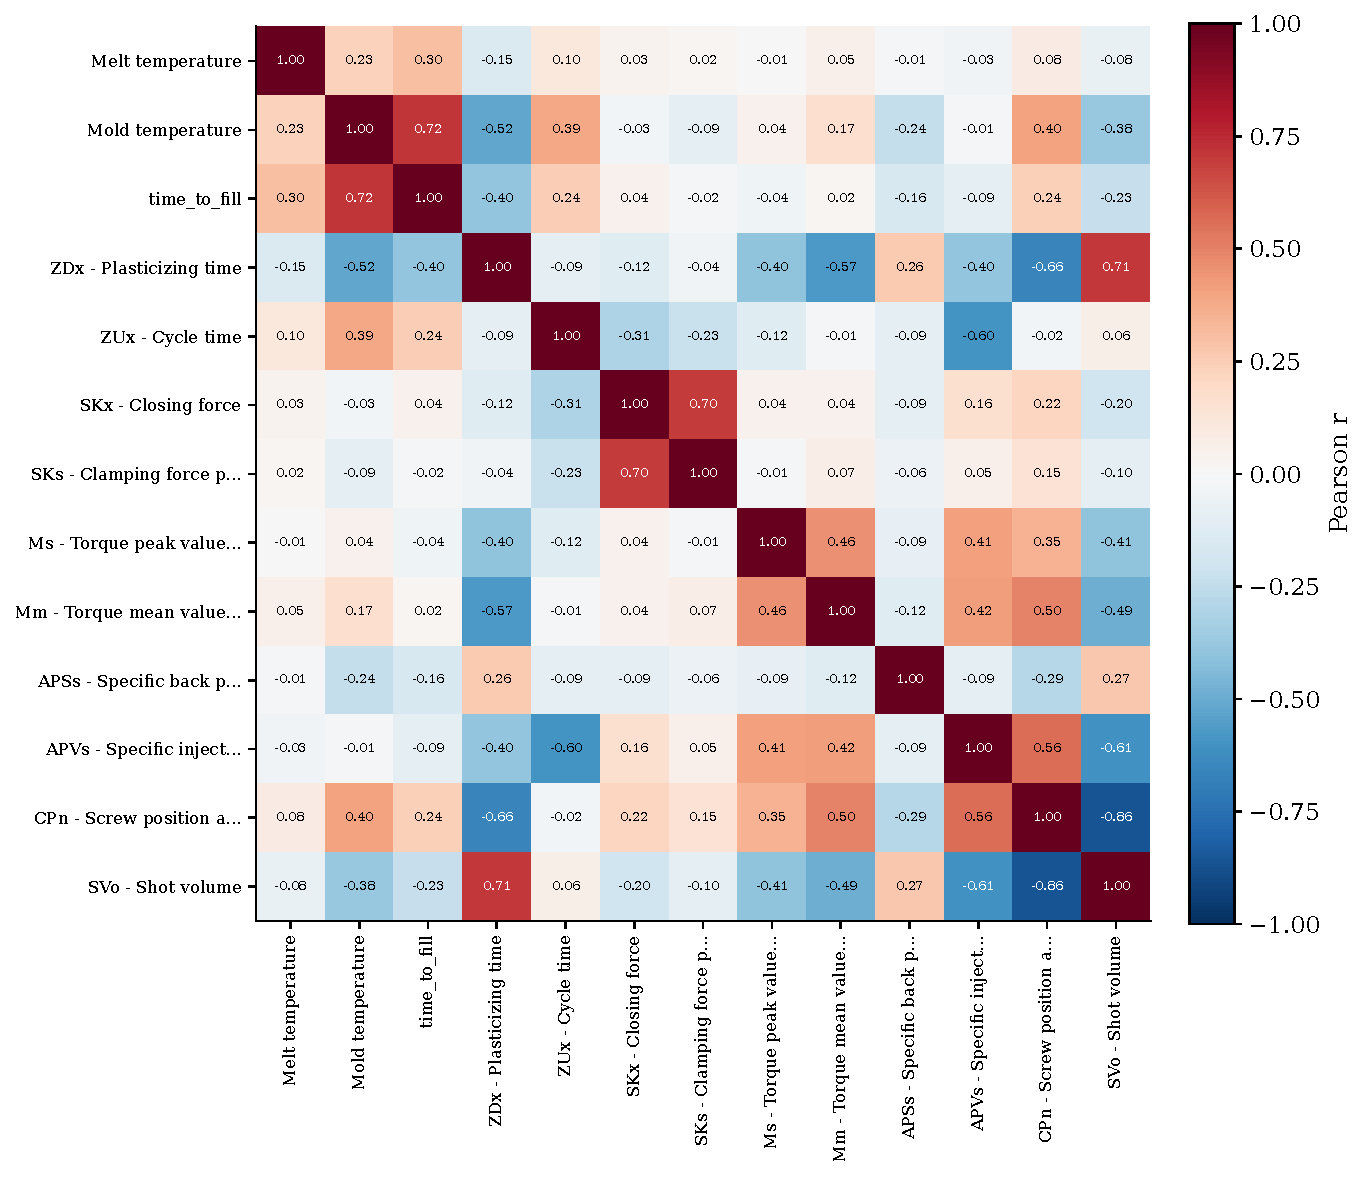
\includegraphics[width=0.75\textwidth]{figures/ch3/fig_ch3_correlation_heatmap.pdf}
\caption{Pearson correlation matrix of the 13 process parameters, training split. Source: \texttt{thesis\_assets/data/correlation\_matrix.csv}, \texttt{thesis\_assets/figures/ch3/fig\_ch3\_correlation\_heatmap}.}
\label{fig:ch3-correlation-heatmap}
\end{figure}

\hypertarget{a.2-setpoint-versus-measured-outcome-classification}{%
\section{A.2 Setpoint versus Measured-Outcome Classification}\label{a.2-setpoint-versus-measured-outcome-classification}}

Section 5.1.3 established a distinction that has no consequence for classification but a substantial one for counterfactual recommendation: some of these quantities are values an operator sets on the machine controller, while others are values the machine measures as a consequence of the cycle. A recommendation to change a measured outcome is not directly executable, because there is no field on the control panel corresponding to it.

\textbf{Table A.2.} Provisional classification of the thirteen parameters by controllability. \textbf{This classification is inferred from the parameter descriptions and from general injection molding practice; it has not been verified against the Engel E-MAC 310/100 controller documentation and should be confirmed before being relied upon.} It is the basis of the setpoint-restriction experiment proposed in §6.4 (F2).

\begin{longtable}[]{@{}
  >{\raggedright\arraybackslash}p{(\columnwidth - 4\tabcolsep) * \real{0.3333}}
  >{\raggedright\arraybackslash}p{(\columnwidth - 4\tabcolsep) * \real{0.3333}}
  >{\raggedright\arraybackslash}p{(\columnwidth - 4\tabcolsep) * \real{0.3333}}@{}}
\toprule\noalign{}
\begin{minipage}[b]{\linewidth}\raggedright
Parameter
\end{minipage} & \begin{minipage}[b]{\linewidth}\raggedright
Classification
\end{minipage} & \begin{minipage}[b]{\linewidth}\raggedright
Basis
\end{minipage} \\
\midrule\noalign{}
\endhead
\bottomrule\noalign{}
\endlastfoot
Melt temperature & Setpoint & Barrel zone temperature is directly set \\
Mold temperature & Setpoint & Mold temperature controller setpoint \\
SKx -- Closing force & Setpoint & Clamp force is configured per job \\
SVo -- Shot volume & Setpoint & Shot size / metering stroke is configured \\
time\_to\_fill & Partly derived & Consequence of the injection speed profile; measured per cycle \\
ZDx -- Plasticizing time & Derived & Consequence of screw rotation speed and back pressure \\
ZUx -- Cycle time & Derived & Aggregate of injection, hold, cooling and mold movement times \\
SKs -- Clamping force peak value & Measured & Peak of the realised clamping force \\
Ms -- Torque peak value & Measured & Peak screw torque during plasticizing \\
Mm -- Torque mean value & Measured & Mean screw torque during plasticizing \\
APSs -- Specific back pressure peak & Measured & Peak of the realised back pressure \\
APVs -- Specific injection pressure peak & Measured & Peak of the realised injection pressure \\
CPn -- Screw position at end of hold & Measured & Realised screw position at hold-pressure cut-off \\
\end{longtable}

Four parameters are cleanly settable; the remaining nine are wholly or partly consequences of the cycle. The three parameters that dominate the SHAP ranking (§4.3.1) --- cycle time, plasticizing time and filling time --- all fall in the derived group.

\hypertarget{a.3-note-on-unit-conventions}{%
\section{A.3 Note on Unit Conventions}\label{a.3-note-on-unit-conventions}}

Two of the recorded parameters carry values that appear inconsistent with typical engineering magnitudes for the units stated in the source publication. This is recorded here as a data-provenance observation, not as a claimed error in the source.

\textbf{Closing and clamping force.} These are stated in newtons and recorded at approximately 900--950. The machine identified in the source publication is an Engel E-MAC 310/100, whose designation indicates a clamping force in the region of 100 metric tonnes, or approximately 1,000 kN. A recorded value of 908 is therefore consistent with \textbf{kilonewtons} rather than newtons --- placing the process at roughly 90\% of the machine's rated clamping force, which is an unremarkable operating point.

\textbf{Melt temperature.} This is stated in degrees Celsius and recorded with a mean of 106.9 °C. Melt temperatures for optical thermoplastics used in road lenses are typically in the range 220--300 °C. The recorded quantity may therefore be a specific barrel zone, a controller-internal scaled value, or a differential rather than an absolute melt temperature.

\textbf{Consequence for this work: none, and this is worth being precise about.} Every method in this thesis operates on the values exactly as recorded, and every recommendation is expressed in the same units and on the same scale as the input. The counterfactual engine's bound enforcement (§3.6.5) clips to the observed range of the recorded values, so no recommendation departs from the range the machine was actually operated at, whatever the units of that range denote.

\textbf{Consequence for deployment: material.} Before any recommendation produced by this framework is transferred to a physical machine, the unit convention of every parameter must be confirmed against the machine's own controller documentation. A recommendation to reduce closing force by 4.18 units is a 0.46\% adjustment if the unit is kN and a physically meaningless one if it is N. This is recorded as a precondition of the physical validation trial specified in §6.4 (F1).

\hypertarget{a.4-feature-name-consistency}{%
\section{A.4 Feature Name Consistency}\label{a.4-feature-name-consistency}}

The exact feature-name strings below are asserted in the test suite (\texttt{tests/test\_data.py}, \texttt{EXPECTED\_FEATURES}) and must match the dataset column headers, the persisted \texttt{feature\_names.pkl} artefact, and every reference in the source code. Any divergence causes a key-lookup failure at run time rather than a silent error.

\begin{verbatim}
Melt temperature
Mold temperature
time_to_fill
ZDx - Plasticizing time
ZUx - Cycle time
SKx - Closing force
SKs - Clamping force peak value
Ms - Torque peak value current cycle
Mm - Torque mean value current cycle
APSs - Specific back pressure peak value
APVs - Specific injection pressure peak value
CPn - Screw position at the end of hold pressure
SVo - Shot volume
\end{verbatim}

Note the inconsistent naming convention inherited from the source dataset: \texttt{time\_to\_fill} uses lowercase snake case while the remaining twelve use the machine's abbreviation code followed by a hyphen-separated description, and two use plain English. The names are reproduced unmodified rather than normalised, so that the dataset as published and the dataset as consumed remain byte-identical.

\hypertarget{hyperparameter-provenance-and-deviation-analysis}{%
\chapter{Hyperparameter Provenance and Deviation Analysis}\label{hyperparameter-provenance-and-deviation-analysis}}

This appendix reproduces the provenance document maintained in the project repository at \texttt{docs/hyperparameter\_provenance.md}. It records the origin of every hyperparameter of the champion Random Forest, classifies each difference from the source configuration, and justifies each deviation. It is reproduced in full because §3.4.3 summarises it and a reader assessing the reproduction claim requires the complete record.

\hypertarget{b.1-reference}{%
\section{B.1 Reference}\label{b.1-reference}}

Polenta, A.; Tomassini, S.; Falcionelli, N.; Contardo, P.; Dragoni, A. F.; Sernani, P. ``A Comparison of Machine Learning Techniques for the Quality Classification of Molded Products.'' \emph{Information}, 2022, 13(6), article 272. DOI: 10.3390/info13060272. Cited in this thesis as reference {[}5{]}.

\hypertarget{b.2-what-the-source-publication-reports}{%
\section{B.2 What the Source Publication Reports}\label{b.2-what-the-source-publication-reports}}

The following values are taken directly from the source, Section 3.2.3 and Table 5. Nothing in this section is inferred.

\begin{itemize}
\tightlist
\item
  \textbf{Best configuration:} 95.04\% ± 1.26\% mean test accuracy via stratified five-fold cross-validation over all 1,451 samples. Parameters: \textbf{151 trees}, \textbf{maximum depth 79}, \textbf{gain ratio} as the splitting criterion.
\item
  \textbf{Second-best configuration:} 94.68\% accuracy. Parameters: \textbf{151 trees}, \textbf{maximum depth 140}, \textbf{information gain} as the splitting criterion.
\item
  \textbf{Ensemble method:} Extremely Randomised Trees (ExtraTrees), in which split thresholds are selected at random rather than greedily optimised.
\item
  \textbf{Features evaluated per split:} int(log(m) + 1), where m is the number of features and log is the natural logarithm. For m = 13: int(ln 13 + 1) = int(3.565) = \textbf{3}.
\item
  \textbf{Minimal leaf size:} 2. \textbf{Minimal size for splitting:} 4. \textbf{Minimal gain:} 0.01.
\item
  \textbf{No pruning strategy} was applied.
\item
  \textbf{Voting:} confidence voting, predicting the class with the highest accumulated confidence summed across trees.
\end{itemize}

\hypertarget{b.3-mapping-table}{%
\section{B.3 Mapping Table}\label{b.3-mapping-table}}

\textbf{Table B.1.} Champion Random Forest hyperparameter provenance, with each difference classified.

\begin{longtable}[]{@{}
  >{\raggedright\arraybackslash}p{(\columnwidth - 6\tabcolsep) * \real{0.2500}}
  >{\raggedright\arraybackslash}p{(\columnwidth - 6\tabcolsep) * \real{0.2500}}
  >{\raggedright\arraybackslash}p{(\columnwidth - 6\tabcolsep) * \real{0.2500}}
  >{\raggedright\arraybackslash}p{(\columnwidth - 6\tabcolsep) * \real{0.2500}}@{}}
\toprule\noalign{}
\begin{minipage}[b]{\linewidth}\raggedright
Hyperparameter
\end{minipage} & \begin{minipage}[b]{\linewidth}\raggedright
Polenta et al.~(2022)
\end{minipage} & \begin{minipage}[b]{\linewidth}\raggedright
This implementation
\end{minipage} & \begin{minipage}[b]{\linewidth}\raggedright
Status
\end{minipage} \\
\midrule\noalign{}
\endhead
\bottomrule\noalign{}
\endlastfoot
\texttt{n\_estimators} & 151 & 151 & \textbf{Identical} \\
\texttt{min\_samples\_leaf} & 2 & 2 & \textbf{Identical} \\
\texttt{min\_samples\_split} & 4 & 4 & \textbf{Identical} \\
\texttt{criterion} & gain ratio (best config) & \texttt{\textquotesingle{}entropy\textquotesingle{}} (information gain) & \textbf{Deviation} --- §B.4.1 \\
\texttt{max\_depth} & 79 (gain ratio row) / 140 (information gain row) & 79 & \textbf{Deviation} --- §B.4.2 \\
Ensemble type & ExtraTrees & \texttt{RandomForestClassifier} & \textbf{Deviation} --- §B.4.3 \\
Features per split & int(ln(m)+1) = 3 for m = 13 & \texttt{\textquotesingle{}sqrt\textquotesingle{}} → int(√13) = 3 & \textbf{Equivalent} --- §B.4.4 \\
Evaluation protocol & 5-fold CV, full dataset & Single held-out split & \textbf{Deviation} --- §B.4.5 \\
\texttt{random\_state} & Not specified & 42 & \textbf{Addition} (reproducibility) \\
\end{longtable}

\hypertarget{b.4-deviation-justifications}{%
\section{B.4 Deviation Justifications}\label{b.4-deviation-justifications}}

\hypertarget{b.4.1-splitting-criterion}{%
\subsection{B.4.1 Splitting Criterion}\label{b.4.1-splitting-criterion}}

The source's best-performing configuration uses the \textbf{gain ratio} criterion, which normalises information gain by split entropy to correct for high-cardinality features. scikit-learn's \texttt{RandomForestClassifier} implements only \texttt{\textquotesingle{}gini\textquotesingle{}} (Gini impurity) and \texttt{\textquotesingle{}entropy\textquotesingle{}} (information gain); gain ratio is not available.

\texttt{criterion=\textquotesingle{}entropy\textquotesingle{}} corresponds to information gain, which is the criterion from the source's \textbf{second-best} row. The source reports a 0.36 percentage-point difference between gain ratio (95.04\%) and information gain (94.68\%) within its own evaluation protocol. \textbf{This magnitude represents an upper bound on what is attributable to the criterion difference} under that protocol.

\hypertarget{b.4.2-maximum-depth}{%
\subsection{B.4.2 Maximum Depth}\label{b.4.2-maximum-depth}}

Two rows of the source's Table 5 are relevant: the gain ratio row specifies \texttt{max\_depth\ =\ 79}, and the information gain row specifies \texttt{max\_depth\ =\ 140}. This work uses \texttt{criterion=\textquotesingle{}entropy\textquotesingle{}} (information gain, §B.4.1) but \texttt{max\_depth=79} (the gain ratio row). The two parameters therefore originate from different rows.

Rather than leaving this as an unresolved inconsistency, it was tested empirically. \texttt{scripts/check\_tree\_depth.py} trains the champion and measures the realised depth of each of its 151 estimators.

\textbf{Table B.2.} Configured versus realised tree depth. Source: \texttt{models/tree\_depth.json}.

\begin{longtable}[]{@{}ll@{}}
\toprule\noalign{}
Statistic & Value \\
\midrule\noalign{}
\endhead
\bottomrule\noalign{}
\endlastfoot
Configured \texttt{max\_depth} & 79 \\
Realised maximum depth & \textbf{20} \\
Realised mean depth & 12.04 \\
Realised median depth & 12.0 \\
Realised minimum depth & 9 \\
Constraint binding? & \textbf{No} \\
\end{longtable}

No tree reaches depth 20, let alone 79 or 140. With 870 training samples, \texttt{min\_samples\_leaf=2} and \texttt{min\_samples\_split=4}, trees terminate naturally well below either bound. \textbf{The discrepancy between 79 and 140 is therefore empirically immaterial on this dataset: both values produce identical trained models.} This resolves the ambiguity rather than merely flagging it, and is the reason the deviation is documented rather than corrected.

\hypertarget{b.4.3-ensemble-type}{%
\subsection{B.4.3 Ensemble Type}\label{b.4.3-ensemble-type}}

The source uses \textbf{Extremely Randomised Trees} {[}82{]}, in which the split threshold for each candidate feature is drawn uniformly at random rather than optimised. \texttt{RandomForestClassifier} selects the best threshold among a random subsample of features, which is a more deterministic search.

\texttt{RandomForestClassifier} is used here for two reasons:

\begin{enumerate}
\def\labelenumi{\arabic{enumi}.}
\tightlist
\item
  \textbf{Downstream compatibility.} The entire explanation and counterfactual chain --- TreeSHAP attribution, SHAP-driven feature selection, LIME direction assignment, the tier cascade, and the independent verifier --- was developed and tested against \texttt{RandomForestClassifier}. Substituting the ensemble type would require re-validating every downstream component, and the risk of a silent behavioural change in the counterfactual engine outweighs the benefit of exact correspondence with the source's ensemble type.
\item
  \textbf{Stack consistency.} All five non-XGBoost candidates in this work use scikit-learn estimators.
\end{enumerate}

\hypertarget{b.4.4-features-evaluated-per-split}{%
\subsection{B.4.4 Features Evaluated Per Split}\label{b.4.4-features-evaluated-per-split}}

The source specifies int(ln(m) + 1) features per candidate split; scikit-learn's \texttt{max\_features=\textquotesingle{}sqrt\textquotesingle{}} uses int(√m). For \textbf{m = 13}:

\begin{itemize}
\tightlist
\item
  Source formula: int(ln 13 + 1) = int(2.565 + 1) = int(3.565) = \textbf{3}
\item
  This work: int(√13) = int(3.606) = \textbf{3}
\end{itemize}

The two formulae produce identical values at m = 13. \textbf{The ``Equivalent'' classification applies specifically to this dataset and does not hold in general} --- at m = 20, for example, the source formula gives 3 and \texttt{\textquotesingle{}sqrt\textquotesingle{}} gives 4.

\hypertarget{b.4.5-evaluation-protocol}{%
\subsection{B.4.5 Evaluation Protocol}\label{b.4.5-evaluation-protocol}}

The source reports mean test accuracy from \textbf{stratified five-fold cross-validation over all 1,451 samples} (95.04\% ± 1.26\%). This work reports cross-validation accuracy on the training split only (n = 870) and a separate held-out test accuracy (n = 291, 93.81\%).

\textbf{The two figures are not directly comparable.} The denominators, the train/test compositions, and the averaging procedures all differ. Any statement placing this work's accuracy alongside the source's 95.04\% must acknowledge this. \textbf{The source's 95.04\% is the reference point for the hyperparameter configuration, not a benchmark this work claims to match or exceed.} See §1.5.2 and §4.2.5.

\hypertarget{b.5-champion-selection}{%
\section{B.5 Champion Selection}\label{b.5-champion-selection}}

The champion is selected by the highest stratified five-fold cross-validation mean accuracy among all six candidates, implemented in \texttt{get\_champion()} in \texttt{src/experiment\_tracker.py}, which ranks on \texttt{cv\_mean} rather than single-split \texttt{val\_acc}.

\textbf{Table B.3.} Six-algorithm comparison. Source: \texttt{models/experiments.json}.

\begin{longtable}[]{@{}llll@{}}
\toprule\noalign{}
Algorithm & CV mean & CV std & Validation accuracy \\
\midrule\noalign{}
\endhead
\bottomrule\noalign{}
\endlastfoot
\textbf{RF} & \textbf{0.9471} & 0.0190 & 0.9310 \\
XGB & 0.9425 & 0.0202 & \textbf{0.9414} \\
GB & 0.9379 & 0.0168 & 0.9310 \\
MLP & 0.9218 & 0.0240 & 0.8931 \\
DT & 0.9023 & 0.0170 & 0.8966 \\
KNN & 0.8839 & 0.0043 & 0.8828 \\
\end{longtable}

Random Forest achieves the highest CV mean (0.9471) and is selected as champion. XGBoost achieves the highest single-split validation accuracy (0.9414), which is precisely why the selection criterion is the cross-validation mean: a single held-out split of 290 samples can be misleading at this resolution, and the difference between the two models on that split is approximately three samples. The full argument is given in §3.4.4.

Held-out test accuracy of the champion (n = 291): \textbf{93.81\%}, from \texttt{models/test\_evaluation.json}.

\hypertarget{b.6-hyperparameters-of-the-non-champion-candidates}{%
\section{B.6 Hyperparameters of the Non-Champion Candidates}\label{b.6-hyperparameters-of-the-non-champion-candidates}}

The five non-champion candidates use library defaults except where the source publication specifies otherwise. Because none is selected as champion, their configurations affect only the ranking, and the ranking's purpose in this work is to justify the champion selection rather than to establish a definitive algorithm comparison. Their exact configurations are recorded in \texttt{models/experiments.json} alongside their results.

\hypertarget{b.7-summary-statement}{%
\section{B.7 Summary Statement}\label{b.7-summary-statement}}

\textbf{The champion's hyperparameters are adopted from the source publication with five documented differences. They are not tuned in this work, and no hyperparameter search was conducted.} This is stated plainly in §3.4.3 and again here, because presenting adopted values as though they were the product of a search conducted in this work would misrepresent it. The consequence --- that a tuned configuration might classify better, and might produce a differently-shaped decision surface with different counterfactual behaviour --- is recorded as limitation L4 in §5.4.

\hypertarget{expert-evaluation-questionnaire-instrument}{%
\chapter{Expert Evaluation Questionnaire Instrument}\label{expert-evaluation-questionnaire-instrument}}

This appendix reproduces the instrument designed for the expert evaluation sub-study specified in §3.9.6 and reported in §4.8. It is reproduced in full whether or not responses were collected, so that the design is auditable and the study replicable.

\begin{center}\rule{0.5\linewidth}{0.5pt}\end{center}

\hypertarget{c.1-administration-notes-not-shown-to-participants}{%
\section{C.1 Administration Notes (not shown to participants)}\label{c.1-administration-notes-not-shown-to-participants}}

\textbf{Purpose.} To assess whether the system's explanations and corrective recommendations are intelligible and credible to people with domain expertise in injection molding or industrial quality control.

\textbf{Design principle --- the verifier's verdict is withheld.} Participants see two RCA cases: one that the independent verifier confirmed and one that it did not. \textbf{Participants are not told which is which, and are not told that a verifier exists.} This is the analytically central feature of the design: it tests whether expert judgement independently distinguishes the cases the verifier distinguishes. Disclosing the verdict would anchor the responses and destroy the comparison.

\textbf{Case order is counterbalanced.} Half of participants receive the confirmed case first (Case A = test index 39), half receive the unconfirmed case first (Case A = test index 5), to control for order effects.

\textbf{Language.} The instrument may be administered in Arabic or English at the participant's preference. If translated, the translation should be reviewed by a second Arabic-speaking engineer for terminological accuracy, and the language used recorded with each response.

\textbf{Estimated completion time.} 20--25 minutes.

\textbf{Analysis.} Descriptive only --- per-construct medians and full response distributions, plus a within-participant comparison of ratings between the confirmed and unconfirmed cases. \textbf{No significance testing is performed}, for the reasons given in §3.9.6 and §4.8.4.

\begin{center}\rule{0.5\linewidth}{0.5pt}\end{center}

\hypertarget{c.2-participant-information-and-consent}{%
\section{C.2 Participant Information and Consent}\label{c.2-participant-information-and-consent}}

\begin{quote}
\textbf{Study title:} Evaluating the interpretability of an AI-based quality control system for injection molding

\textbf{Researcher:} Obadah AlQawasema, Intelligent Systems Master Program, Palestine Polytechnic University
\textbf{Supervisor:} \emph{{[}Insert name{]}}

\textbf{What this study is about.} You are being invited to review the output of a software system that predicts the quality of injection-molded parts from machine process data, explains its predictions, and recommends corrective parameter adjustments. We would like your professional judgement on whether that output is clear and credible.

\textbf{What you will be asked to do.} You will be shown two production cycles. For each, you will see the machine's recorded process parameters, the system's quality classification, an explanation of which parameters drove that classification, and the adjustments the system recommends. You will then answer several rating questions and, if you wish, add comments. This takes approximately 20--25 minutes.

\textbf{There are no right or wrong answers.} We are evaluating the system, not you. Critical responses are as valuable as positive ones and more useful to the research.

\textbf{What we record.} Your responses, your professional role, and your years of experience in a broad band. \textbf{We do not record your name, your employer, or any other identifying information.} Results are reported only in aggregate, and no response will be attributable to an individual.

\textbf{Voluntary participation.} Participation is entirely voluntary. You may decline to answer any question and may stop at any point without giving a reason and without consequence.

\textbf{Use of results.} Aggregated, anonymous results will appear in a Master's thesis submitted to Palestine Polytechnic University and may appear in subsequent academic publication.

\textbf{Questions.} \emph{{[}Insert researcher contact e-mail{]}}

$\square$ I have read and understood the above, and I agree to take part.
\end{quote}

\begin{center}\rule{0.5\linewidth}{0.5pt}\end{center}

\hypertarget{c.3-section-1-background-3-items}{%
\section{C.3 Section 1 --- Background (3 items)}\label{c.3-section-1-background-3-items}}

\textbf{B1.} Which best describes your current role?
$\square$ Process engineer $\square$ Quality manager or quality engineer $\square$ Machine operator or technician $\square$ Production manager $\square$ Academic or researcher $\square$ Other: \_\_\_\_\_\_

\textbf{B2.} How many years have you worked with injection molding or plastics processing?
$\square$ Under 2 $\square$ 2--5 $\square$ 6--10 $\square$ 11--20 $\square$ Over 20

\textbf{B3.} How would you describe your prior experience with AI or machine learning tools in a production setting?
$\square$ None $\square$ Have read about them $\square$ Have used one $\square$ Have deployed or maintained one

\begin{center}\rule{0.5\linewidth}{0.5pt}\end{center}

\hypertarget{c.4-section-2-case-presentation}{%
\section{C.4 Section 2 --- Case Presentation}\label{c.4-section-2-case-presentation}}

\emph{Each case is presented on its own page in the following format. The two cases are drawn from the held-out test split of the road-lens dataset and are reproduced exactly as the system generated them.}

\begin{quote}
\hypertarget{case-a-b}{%
\subsection{Case {[}A / B{]}}\label{case-a-b}}

\textbf{Recorded process parameters for this production cycle}

\emph{{[}Table of all thirteen parameters with their recorded values in engineering units, as specified in Appendix A.{]}}

\textbf{System classification:} \emph{{[}e.g.~Waste --- non-conforming{]}}
\textbf{System confidence that the part conforms:} \emph{{[}e.g.~15.7\%{]}}

\textbf{Explanation --- the parameters the system identified as most influential for this cycle:}

\emph{{[}The five top-ranked parameters by local attribution, with the direction of each parameter's influence.{]}}

\textbf{Recommended adjustments}

\begin{longtable}[]{@{}lllll@{}}
\toprule\noalign{}
Parameter & Current & Suggested & Change & Direction \\
\midrule\noalign{}
\endhead
\bottomrule\noalign{}
\endlastfoot
\emph{{[}five rows, engineering units{]}} & & & & \\
\end{longtable}

\textbf{System confidence after the recommended adjustments:} \emph{{[}e.g.~74.3\%{]}}
\end{quote}

\textbf{Case source data.} The confirmed case is test-split index 39, reproduced as Table 4.16. The unconfirmed case is test-split index 5, recorded in \texttt{thesis\_assets/data/counterfactual\_cases.json}. Both are genuine system outputs; neither has been edited.

\begin{center}\rule{0.5\linewidth}{0.5pt}\end{center}

\hypertarget{c.5-section-3-rating-items-per-case}{%
\section{C.5 Section 3 --- Rating Items (per case)}\label{c.5-section-3-rating-items-per-case}}

\emph{Each item is answered on a five-point scale: 1 = Strongly disagree, 2 = Disagree, 3 = Neither agree nor disagree, 4 = Agree, 5 = Strongly agree.}

\textbf{Table C.1.} Likert constructs and their items.

\begin{longtable}[]{@{}
  >{\raggedright\arraybackslash}p{(\columnwidth - 4\tabcolsep) * \real{0.3333}}
  >{\raggedright\arraybackslash}p{(\columnwidth - 4\tabcolsep) * \real{0.3333}}
  >{\raggedright\arraybackslash}p{(\columnwidth - 4\tabcolsep) * \real{0.3333}}@{}}
\toprule\noalign{}
\begin{minipage}[b]{\linewidth}\raggedright
Code
\end{minipage} & \begin{minipage}[b]{\linewidth}\raggedright
Construct
\end{minipage} & \begin{minipage}[b]{\linewidth}\raggedright
Item wording
\end{minipage} \\
\midrule\noalign{}
\endhead
\bottomrule\noalign{}
\endlastfoot
\textbf{C1} & Explanation clarity & The explanation makes it clear which process parameters drove this classification. \\
\textbf{C2} & Recommendation plausibility & The recommended adjustments are plausible as a process intervention on a real machine. \\
\textbf{C3} & Behavioural intention & I would be willing to apply these adjustments on a running machine. \\
\textbf{C4} & System trust & I would trust a system of this kind as a decision-support tool in quality control. \\
\end{longtable}

Each rating item is followed by:

\begin{quote}
\textbf{Please explain your rating briefly.} (free text) \_\_\_\_\_\_\_\_\_\_\_\_\_\_\_\_\_\_\_\_\_\_
\end{quote}

Two further per-case items:

\textbf{C5.} Are there any parameters you would have expected the system to change that it did not? (free text)

\textbf{C6.} Are there any recommended changes that you consider unwise, impractical, or impossible on a real machine? If so, which, and why? (free text)

\emph{Item C6 is the most diagnostically important free-text field. It is the only route by which a participant can surface the setpoint-versus-measured-outcome problem identified in §5.1.3 without being prompted toward it.}

\begin{center}\rule{0.5\linewidth}{0.5pt}\end{center}

\hypertarget{c.6-section-4-overall-items-asked-once-after-both-cases}{%
\section{C.6 Section 4 --- Overall Items (asked once, after both cases)}\label{c.6-section-4-overall-items-asked-once-after-both-cases}}

\textbf{O1.} Considering both cases, which of the two sets of recommendations did you find more credible?
$\square$ Case A $\square$ Case B $\square$ About the same $\square$ Neither was credible

\textbf{O2.} Please explain your answer to O1. (free text)

\emph{Items O1--O2 are the primary analytical instrument of the sub-study. Whether expert judgement aligns with the independent verifier's verdict is the question these two items exist to answer.}

\textbf{O3.} In your view, how should output of this kind be presented to a machine operator?
$\square$ As an instruction to carry out
$\square$ As a suggestion to consider
$\square$ As one input among several, alongside the operator's own judgement
$\square$ It should not be shown to operators at all
$\square$ Other: \_\_\_\_\_\_

\textbf{O4.} What would have to be true for you to rely on a system of this kind in your own work? (free text)

\textbf{O5.} Any other comments on the system, the explanations, or the recommendations. (free text)

\begin{center}\rule{0.5\linewidth}{0.5pt}\end{center}

\hypertarget{c.7-response-recording-template}{%
\section{C.7 Response Recording Template}\label{c.7-response-recording-template}}

\begin{longtable}[]{@{}ll@{}}
\toprule\noalign{}
Field & Values \\
\midrule\noalign{}
\endhead
\bottomrule\noalign{}
\endlastfoot
Participant code & P01, P02, \ldots{} (sequential; no link to identity) \\
Role (B1), Experience band (B2), AI exposure (B3) & --- \\
Case order received & Confirmed-first / Unconfirmed-first \\
Language of administration & Arabic / English \\
C1--C4 per case & 1--5 \\
C5, C6 per case & Free text \\
O1--O5 & --- \\
Date of completion & --- \\
\end{longtable}

\begin{center}\rule{0.5\linewidth}{0.5pt}\end{center}

\hypertarget{c.8-known-limitations-of-the-instrument}{%
\section{C.8 Known Limitations of the Instrument}\label{c.8-known-limitations-of-the-instrument}}

These are stated here, and again in §4.8.4, so that the instrument is not read as stronger than it is.

\textbf{It measures credibility, not correctness.} Expert plausibility judgement and recommendation correctness are different constructs. An expert may find a recommendation plausible and be wrong; a correct recommendation may be counter-intuitive. This instrument complements the independent-validation protocol of §3.9.3 and cannot substitute for it.

\textbf{It measures reading, not use.} Participants judge a static case presentation rather than using the running system, so the results speak to the intelligibility of the output rather than to the usability of the application.

\textbf{Two cases cannot establish a pattern.} Items O1--O2 test whether expert judgement aligns with the verifier's verdict on a single pair. A properly powered version of that test would require many stratified pairs per participant, which the estimated completion time does not permit.

\textbf{The sample is not random.} Participants recruited through professional contacts may be more favourably disposed toward digital quality tools than the population a deployment would encounter.

\hypertarget{artefact-index}{%
\chapter{Artefact Index}\label{artefact-index}}

Every quantitative claim in this thesis traces to a file in the project repository, and every such file traces to the script that produced it and the data it consumed. This appendix reproduces that mapping. It is derived from \texttt{thesis\_assets/MANIFEST.md} and \texttt{models/ARTIFACTS.md}.

\textbf{Repository:} \texttt{github.com/obadaqw/Thesis\_Industrial\_AI\_V2}

\hypertarget{d.1-reproduction-procedure}{%
\section{D.1 Reproduction Procedure}\label{d.1-reproduction-procedure}}

The complete result set regenerates from raw data in two stages:

\begin{verbatim}
# Stage 1 — all evaluation artefacts (~3–4 h on CPU)
bash scripts/run_all_evaluations.sh

# Stage 2 — all thesis figures and tables
bash scripts/build_thesis_assets.sh
\end{verbatim}

Stage 1 executes, in dependency order: the data pipeline; training of all six candidate algorithms; the tree-depth verification; test-set evaluation; RCA batch evaluation on the validation and test splits; the tier sensitivity sweep on both splits; the method comparison on both splits; and the drift validation sweep. Stage 2 executes: dataset statistics export; XAI batch export; RCA worked-case export; Quality 4.0 module export; figure generation; and table export.

\textbf{Non-overwriting outputs.} Evaluation scripts write to split-suffixed filenames and do not overwrite existing results, so a re-run cannot silently replace a figure already cited in this thesis.

\textbf{Seeds.} 42 for the data split and champion model; 7 for the independent verifier; 42 for the SHAP beeswarm subsample.

\hypertarget{d.2-key-results-summary}{%
\section{D.2 Key Results Summary}\label{d.2-key-results-summary}}

\textbf{Table D.1.} Headline figures and their source files.

\begin{longtable}[]{@{}
  >{\raggedright\arraybackslash}p{(\columnwidth - 4\tabcolsep) * \real{0.3333}}
  >{\raggedright\arraybackslash}p{(\columnwidth - 4\tabcolsep) * \real{0.3333}}
  >{\raggedright\arraybackslash}p{(\columnwidth - 4\tabcolsep) * \real{0.3333}}@{}}
\toprule\noalign{}
\begin{minipage}[b]{\linewidth}\raggedright
Metric
\end{minipage} & \begin{minipage}[b]{\linewidth}\raggedright
Value
\end{minipage} & \begin{minipage}[b]{\linewidth}\raggedright
Source file
\end{minipage} \\
\midrule\noalign{}
\endhead
\bottomrule\noalign{}
\endlastfoot
RF cross-validation mean accuracy (5-fold, training split) & 94.71\% & \texttt{models/experiments.json} \\
RF held-out test accuracy (n = 291) & \textbf{93.81\%} & \texttt{models/test\_evaluation.json} \\
\emph{Waste} recall, test split & 94.59\% & \texttt{models/test\_evaluation.json} \\
Non-conformance recall, test split & 94.56\% & \texttt{models/test\_evaluation.json} \\
RCA resolution rate, validation split & 97.96\% & \texttt{models/rca\_evaluation\_val.json} \\
RCA resolution rate, test split & \textbf{95.24\%} & \texttt{models/rca\_evaluation\_test.json} \\
Validator agreement rate, validation split & 11.11\% & \texttt{models/rca\_evaluation\_val.json} \\
Validator agreement rate, test split & \textbf{6.43\%} & \texttt{models/rca\_evaluation\_test.json} \\
3-tier vs.~ablation sparsity, validation & 4.9 vs.~12.4 features & \texttt{models/rca\_comparison\_val.json} \\
3-tier vs.~ablation sparsity, test & 4.9 vs.~12.3 features & \texttt{models/rca\_comparison\_test.json} \\
McNemar exact p, validation split & 0.625 (not significant) & \texttt{models/rca\_comparison\_val.json} \\
McNemar exact p, test split & \textbf{0.180 (not significant)} & \texttt{models/rca\_comparison\_test.json} \\
PSI trigger magnitude & k = 1σ, all 13 parameters & \texttt{models/drift\_validation.json} \\
Realised maximum tree depth (configured 79) & 20 & \texttt{models/tree\_depth.json} \\
\end{longtable}

\hypertarget{d.3-chapter-3-assets}{%
\section{D.3 Chapter 3 Assets}\label{d.3-chapter-3-assets}}

\textbf{Table D.2.} Chapter 3 figures and tables.

\begin{longtable}[]{@{}
  >{\raggedright\arraybackslash}p{(\columnwidth - 10\tabcolsep) * \real{0.1667}}
  >{\raggedright\arraybackslash}p{(\columnwidth - 10\tabcolsep) * \real{0.1667}}
  >{\raggedright\arraybackslash}p{(\columnwidth - 10\tabcolsep) * \real{0.1667}}
  >{\raggedright\arraybackslash}p{(\columnwidth - 10\tabcolsep) * \real{0.1667}}
  >{\raggedright\arraybackslash}p{(\columnwidth - 10\tabcolsep) * \real{0.1667}}
  >{\raggedright\arraybackslash}p{(\columnwidth - 10\tabcolsep) * \real{0.1667}}@{}}
\toprule\noalign{}
\begin{minipage}[b]{\linewidth}\raggedright
Asset
\end{minipage} & \begin{minipage}[b]{\linewidth}\raggedright
Type
\end{minipage} & \begin{minipage}[b]{\linewidth}\raggedright
Description
\end{minipage} & \begin{minipage}[b]{\linewidth}\raggedright
Script
\end{minipage} & \begin{minipage}[b]{\linewidth}\raggedright
Source
\end{minipage} & \begin{minipage}[b]{\linewidth}\raggedright
Split
\end{minipage} \\
\midrule\noalign{}
\endhead
\bottomrule\noalign{}
\endlastfoot
\texttt{fig\_ch3\_class\_distribution} & Figure & Class counts across train/val/test & \texttt{generate\_thesis\_figures.py} & \texttt{class\_distribution.json} & all \\
\texttt{fig\_ch3\_correlation\_heatmap} & Figure & 13 × 13 Pearson correlation & \texttt{generate\_thesis\_figures.py} & \texttt{correlation\_matrix.csv} & train \\
\texttt{fig\_ch3\_feature\_ranges} & Figure & Standardised box plot, 13 parameters & \texttt{generate\_thesis\_figures.py} & \texttt{raw\_data.csv} & full \\
\texttt{tbl\_ch3\_feature\_specification} & Table & 13 parameters: unit, min/max/mean/median/std & \texttt{export\_thesis\_tables.py} & \texttt{feature\_specification.json} & full (raw) \\
\texttt{tbl\_ch3\_class\_distribution} & Table & Class counts and percentages, full + per split & \texttt{export\_thesis\_tables.py} & \texttt{class\_distribution.json} & all \\
\texttt{tbl\_ch3\_split\_summary} & Table & Split sizes, proportions, seed, stratification check & \texttt{export\_thesis\_tables.py} & \texttt{split\_summary.json} & all \\
\texttt{tbl\_ch3\_hyperparameter\_provenance} & Table & RF hyperparameter mapping vs.~reference & \texttt{export\_thesis\_tables.py} & \texttt{docs/hyperparameter\_provenance.md} & n/a \\
\texttt{tbl\_ch3\_tree\_depth} & Table & Configured vs.~realised RF tree depth & \texttt{export\_thesis\_tables.py} & \texttt{models/tree\_depth.json} & train \\
\end{longtable}

\hypertarget{d.4-chapter-4-assets}{%
\section{D.4 Chapter 4 Assets}\label{d.4-chapter-4-assets}}

\textbf{Table D.3.} Chapter 4 figures.

\begin{longtable}[]{@{}
  >{\raggedright\arraybackslash}p{(\columnwidth - 6\tabcolsep) * \real{0.2500}}
  >{\raggedright\arraybackslash}p{(\columnwidth - 6\tabcolsep) * \real{0.2500}}
  >{\raggedright\arraybackslash}p{(\columnwidth - 6\tabcolsep) * \real{0.2500}}
  >{\raggedright\arraybackslash}p{(\columnwidth - 6\tabcolsep) * \real{0.2500}}@{}}
\toprule\noalign{}
\begin{minipage}[b]{\linewidth}\raggedright
Asset
\end{minipage} & \begin{minipage}[b]{\linewidth}\raggedright
Section
\end{minipage} & \begin{minipage}[b]{\linewidth}\raggedright
Description
\end{minipage} & \begin{minipage}[b]{\linewidth}\raggedright
Source
\end{minipage} \\
\midrule\noalign{}
\endhead
\bottomrule\noalign{}
\endlastfoot
\texttt{fig\_ch4\_algorithm\_comparison} & 4.2.1 & Six-algorithm CV mean ± std & \texttt{experiments.json} \\
\texttt{fig\_ch4\_confusion\_matrix\_test} & 4.2.4 & 4 × 4 confusion matrix, counts + row \% & \texttt{test\_evaluation.json} \\
\texttt{fig\_ch4\_per\_class\_vs\_baseline} & 4.2.5 & Per-class metrics vs.~reference RF row & \texttt{test\_evaluation.json} + \texttt{POLENTA\_TABLE10\_RF} \\
\texttt{fig\_ch4\_shap\_global\_bar} & 4.3.1 & Mean \textbar SHAP\textbar{} per parameter & \texttt{shap\_global\_importance.json} \\
\texttt{fig\_ch4\_shap\_beeswarm} & 4.3.1 & SHAP summary, \emph{Target} class, 200-sample draw & \texttt{shap\_global\_importance.json} \\
\texttt{fig\_ch4\_shap\_local\_waterfall} & 4.3.3 & Local SHAP, test indices 8, 5, 0 & \texttt{local\_explanations.json} \\
\texttt{fig\_ch4\_lime\_local} & 4.3.3 & LIME coefficients, same three cases & \texttt{local\_explanations.json} \\
\texttt{fig\_ch4\_importance\_method\_comparison} & 4.3.2 & SHAP vs.~Relief vs.~ANOVA ranks & \texttt{shap\_vs\_filters.json} \\
\texttt{fig\_ch4\_top\_adjusted\_features} & 4.4.3 & Adjustment frequency, top five & \texttt{rca\_evaluation\_test.json} \\
\texttt{fig\_ch4\_method\_comparison\_metrics} & 4.5.5 & Proximity, sparsity, NN distance by method & \texttt{rca\_comparison\_test.json} \\
\texttt{fig\_ch4\_validator\_by\_split\_method} & 4.5.3 & Validator rate, both methods × both splits & \texttt{rca\_comparison\_\{val,test\}.json} \\
\texttt{fig\_ch4\_tier\_distribution} & 4.6.1 & RCA outcomes across five thresholds & \texttt{tier\_sensitivity\_test.json} \\
\textbf{\texttt{fig\_ch4\_tradeoff\_resolution\_validator}} & \textbf{4.6.1} & \textbf{Central result figure: resolution vs.~validator agreement across thresholds} & \texttt{tier\_sensitivity\_test.json} \\
\texttt{fig\_ch4\_tradeoff\_maxiter} & 4.6.2 & Same trade-off across iteration budgets & \texttt{tier\_sensitivity\_test.json} \\
\texttt{fig\_ch4\_psi\_sensitivity} & 4.7 & PSI vs.~k·σ shift, 13 parameters & \texttt{drift\_validation.csv} \\
\end{longtable}

\textbf{Table D.4.} Chapter 4 tables.

\begin{longtable}[]{@{}
  >{\raggedright\arraybackslash}p{(\columnwidth - 6\tabcolsep) * \real{0.2500}}
  >{\raggedright\arraybackslash}p{(\columnwidth - 6\tabcolsep) * \real{0.2500}}
  >{\raggedright\arraybackslash}p{(\columnwidth - 6\tabcolsep) * \real{0.2500}}
  >{\raggedright\arraybackslash}p{(\columnwidth - 6\tabcolsep) * \real{0.2500}}@{}}
\toprule\noalign{}
\begin{minipage}[b]{\linewidth}\raggedright
Asset
\end{minipage} & \begin{minipage}[b]{\linewidth}\raggedright
Section
\end{minipage} & \begin{minipage}[b]{\linewidth}\raggedright
Description
\end{minipage} & \begin{minipage}[b]{\linewidth}\raggedright
Source
\end{minipage} \\
\midrule\noalign{}
\endhead
\bottomrule\noalign{}
\endlastfoot
\texttt{tbl\_ch4\_algorithm\_comparison} & 4.2.1 & Six algorithms: CV mean/std, val acc/F1 & \texttt{experiments.json} \\
\texttt{tbl\_ch4\_test\_performance} & 4.2.2 & Headline test metrics & \texttt{test\_evaluation.json} \\
\texttt{tbl\_ch4\_per\_class\_metrics} & 4.2.3 & Precision/recall/support per class & \texttt{test\_evaluation.json} \\
\texttt{tbl\_ch4\_confusion\_matrix} & 4.2.4 & 4 × 4 matrix with totals & \texttt{test\_evaluation.json} \\
\texttt{tbl\_ch4\_baseline\_comparison} & 4.2.5 & This work vs.~reference, with protocol note & \texttt{test\_evaluation.json} \\
\texttt{tbl\_ch4\_shap\_global\_ranking} & 4.3.1 & 13 parameters by mean \textbar SHAP\textbar{} & \texttt{shap\_global\_importance.json} \\
\texttt{tbl\_ch4\_importance\_method\_comparison} & 4.3.2 & SHAP/impurity/Relief/ANOVA + Spearman r & \texttt{shap\_vs\_impurity.json}, \texttt{shap\_vs\_filters.json} \\
\texttt{tbl\_ch4\_rca\_summary} & 4.4.1 & Tier counts, resolution, validator rate, both splits & \texttt{rca\_evaluation\_\{val,test\}.json} \\
\texttt{tbl\_ch4\_counterfactual\_case} & 4.4.4 & Confirmed worked case, engineering units & \texttt{counterfactual\_case\_table.csv} \\
\texttt{tbl\_ch4\_method\_comparison} & 4.5.3 & All five metrics, both methods, both splits, McNemar p & \texttt{rca\_comparison\_\{val,test\}.json} \\
\texttt{tbl\_ch4\_tier\_sensitivity} & 4.6 & All eight sweep configurations, both splits & \texttt{tier\_sensitivity\_\{val,test\}.json} \\
\texttt{tbl\_ch4\_drift\_sensitivity} & 4.7 & PSI at each k·σ per parameter & \texttt{drift\_validation.csv} \\
\end{longtable}

\hypertarget{d.5-supporting-data-exhibits}{%
\section{D.5 Supporting Data Exhibits}\label{d.5-supporting-data-exhibits}}

\textbf{Table D.5.} Narrative exhibits in \texttt{thesis\_assets/data/}.

\begin{longtable}[]{@{}
  >{\raggedright\arraybackslash}p{(\columnwidth - 6\tabcolsep) * \real{0.2500}}
  >{\raggedright\arraybackslash}p{(\columnwidth - 6\tabcolsep) * \real{0.2500}}
  >{\raggedright\arraybackslash}p{(\columnwidth - 6\tabcolsep) * \real{0.2500}}
  >{\raggedright\arraybackslash}p{(\columnwidth - 6\tabcolsep) * \real{0.2500}}@{}}
\toprule\noalign{}
\begin{minipage}[b]{\linewidth}\raggedright
File
\end{minipage} & \begin{minipage}[b]{\linewidth}\raggedright
Feeds
\end{minipage} & \begin{minipage}[b]{\linewidth}\raggedright
Description
\end{minipage} & \begin{minipage}[b]{\linewidth}\raggedright
Split
\end{minipage} \\
\midrule\noalign{}
\endhead
\bottomrule\noalign{}
\endlastfoot
\texttt{feature\_specification.json} & App. A & Per-parameter units and descriptive statistics & raw \\
\texttt{class\_distribution.json} & Ch3 & Class counts and percentages, full and per split & all \\
\texttt{correlation\_matrix.csv} & Ch3 & 13 × 13 Pearson correlation & train \\
\texttt{split\_summary.json} & Ch3 & Split sizes, proportions, seed, stratification check & all \\
\texttt{shap\_global\_importance.json} & Ch4 & Mean \textbar SHAP\textbar, aggregated and per class & train \\
\texttt{shap\_vs\_impurity.json} & Ch4 & SHAP vs.~RF impurity, Spearman r = 1.000 & train \\
\texttt{shap\_vs\_filters.json} & Ch4 & SHAP vs.~Relief (r = 0.659) and ANOVA (r = 0.604) & train / reference \\
\texttt{local\_explanations.json} & Ch4 & Three worked cases: values, probabilities, SHAP, LIME & test \\
\texttt{shap\_lime\_agreement.json} & §4.3.3 & SHAP--LIME rank agreement, 50 test cycles & test \\
\texttt{lime\_stability.json} & §4.3.3 & LIME repeatability, 10 runs on one fixed cycle & test \\
\texttt{xai\_timing.json} & §4.3.4 & SHAP/LIME wall-clock timing, cache hit rate & test \\
\texttt{counterfactual\_cases.json} & §4.4.4 & Three worked RCA cases: confirmed, unconfirmed, Tier-0 & test \\
\texttt{counterfactual\_case\_table.csv} & Table 4.16 & Confirmed case, flattened to engineering units & test \\
\texttt{unresolved\_analysis.json} & §4.4.1 & The 7 excluded cases compared against the 140 resolved & test \\
\texttt{process\_capability.json} & §5.3.4 & Cp/Cpk per parameter --- \textbf{limits ASSUMED, see file header} & full (raw) \\
\texttt{oee\_simulation.json} & §3.7.4 & One representative OEE scenario & test (replayed) \\
\texttt{traceability\_sample.json} & §3.7.2 & Five audit-trail records --- \textbf{see provenance note in file} & test \\
\texttt{llm\_report\_sample.md} & §3.7.5 & One verbatim shift-report exhibit (test index 39) & test \\
\end{longtable}

\hypertarget{d.6-provenance-notes-attached-to-specific-artefacts}{%
\section{D.6 Provenance Notes Attached to Specific Artefacts}\label{d.6-provenance-notes-attached-to-specific-artefacts}}

Three artefacts carry provenance qualifications recorded in the files themselves and reproduced here, because a reader consulting the repository should encounter them at the same time as the data.

\textbf{\texttt{process\_capability.json} --- assumed specification limits.} The USL and LSL values are read from \texttt{config/constraints.yaml}, whose own header records that it was auto-generated from \texttt{raw\_data.csv}. They are therefore the \textbf{observed minimum and maximum of the historical dataset, not sourced customer or engineering specification limits.} Cp and Cpk computed against them are statistics about distribution shape, not capability assessments. See §5.3.4.

\textbf{\texttt{traceability\_sample.json} --- replayed, not logged.} No interactive session had populated \texttt{data/cycle\_history.db} at export time. Rather than fabricate audit records, the export script replayed five genuine, already-computed RCA outcomes from \texttt{models/rca\_results\_test.csv} through the real \texttt{cycle\_store.log\_cycle()} and \texttt{get\_recent()} functions against a throwaway SQLite file. The production database was not written to. No fields required anonymisation: the schema records only timestamp and outcome fields, no operator or personal data.

\textbf{\texttt{fig\_ch4\_per\_class\_vs\_baseline} and \texttt{tbl\_ch4\_baseline\_comparison} --- protocol mismatch.} These compare against the Random Forest row of Polenta et al.~{[}5{]}, Table 10, transcribed verbatim into the \texttt{POLENTA\_TABLE10\_RF} constant in both the figure and table scripts. The reference's values are summed across the five folds of stratified cross-validation over the full 1,451-sample dataset; this work's are from a single held-out split of 291. The comparison is directionally indicative only, and both outputs carry the caveat in their own captions.

\hypertarget{d.7-assets-requiring-manual-production}{%
\section{D.7 Assets Requiring Manual Production}\label{d.7-assets-requiring-manual-production}}

\texttt{thesis\_assets/figures/appendix/} contains a checklist rather than rendered figures. The eight application screenshots of Appendix F require an interactive session and cannot be produced by a script. \texttt{MANIFEST.md}, \texttt{CAPTIONS.md}, and the appendix README are hand-authored and are \textbf{not} regenerated by \texttt{build\_thesis\_assets.sh}; they must not be deleted when regenerating.

\hypertarget{selected-code-listings}{%
\chapter{Selected Code Listings}\label{selected-code-listings}}

This appendix reproduces the source of the three components on which the thesis's central finding depends: the three-tier counterfactual engine, the independent verifier, and the centroid-ablation baseline. Listings are reproduced from the project repository and are abridged where indicated; complete sources are at \texttt{github.com/obadaqw/Thesis\_Industrial\_AI\_V2}.

Peripheral modules --- the Streamlit pages, the LLM wrapper, the notification transport, the digital twin, and the role manager --- are not reproduced here. They are infrastructure (§3.7) and their inclusion would obscure the components that matter.

\begin{center}\rule{0.5\linewidth}{0.5pt}\end{center}

\hypertarget{e.1-counterfactual-rca-engine-configuration-and-contract}{%
\section{E.1 Counterfactual RCA Engine --- Configuration and Contract}\label{e.1-counterfactual-rca-engine-configuration-and-contract}}

\texttt{src/counterfactual\_rca.py}, module header and hyperparameters.

\begin{verbatim}
"""
counterfactual_rca.py — Counterfactual RCA: 3-Tier parameter-correction engine.

Distinct from rca_surrogate.py (Statistical Anomaly Monitor): that module flags
*which sensors / hardware components* deviate statistically; this module computes
*which parameter adjustments* would move a defective cycle into the conforming
region. Tier-3 escalations here correspond to cycles where the anomaly monitor
typically reports structural / multi-sensor faults beyond correctable bounds.

Design decisions implemented:
  #7  SHAP SELECTS which features to adjust (top-k by |SHAP value for Target class|).
      LIME gives the DIRECTION (sign of local linear coefficient for Target class).
  #9  Three-tier strategy in order: T1 -> T2 -> T3 (escalation).
  #10 ROBUST T2: centroid of <=15 nearest real good-quality samples; acceptance
      requires P(Acceptable) + P(Target) >= 0.55 (confidence margin).
  #11 Accepted counterfactual: model predicts class in {1, 2} (Acceptable OR Target).
  #12 Independent MLP validator (random_state=7, family != RF) confirms CF;
      validator_ok flag is returned to the caller/UI.

All counterfactual search is performed in MinMax-scaled space ([-1, 1]).
Physical bounds are enforced via np.clip at every iteration.
"""

# ── Hyper-parameters ─────────────────────────────────────────────────────────
TARGET_CLASSES       = {1, 2}   # model 0-based: 1=Acceptable, 2=Target
CONFIDENCE_THRESHOLD = 0.55     # P(Acceptable) + P(Target) to accept CF
T1_TOP_K             = 5        # SHAP selects top-5 features
T2_TOP_K             = 7        # Tier-2 adjusts top-7 features
T2_N_NEIGHBORS       = 15       # centroid of 15 nearest good samples
STEP                 = 0.02     # per-iteration step in scaled [-1,1] space
MAX_ITER             = 150      # max iterations per tier
LIME_SAMPLES         = 2000     # LIME perturbation budget
\end{verbatim}

\texttt{TARGET\_CLASSES} is the single definition of conformance (§3.2.3). It is imported by \texttt{evaluate\_rca.py}, \texttt{compare\_rca\_methods.py}, \texttt{tier\_sensitivity.py} and \texttt{greedy\_rca.py}, so that one constant governs the entire system.

\begin{center}\rule{0.5\linewidth}{0.5pt}\end{center}

\hypertarget{e.2-acceptance-criterion-and-the-independent-verifier}{%
\section{E.2 Acceptance Criterion and the Independent Verifier}\label{e.2-acceptance-criterion-and-the-independent-verifier}}

\texttt{src/counterfactual\_rca.py}, acceptance and verification helpers.

\begin{verbatim}
    def _confidence(self, x_scaled):
        """P(Acceptable) + P(Target) for a single scaled vector."""
        proba = self.model.predict_proba(x_scaled.reshape(1, -1))\cite{ref0}
        return float(proba\cite{ref1} + proba\cite{ref2})

    def _is_accepted(self, x_scaled):
        return self._confidence(x_scaled) >= self.confidence_threshold

    def _validate(self, x_scaled):
        """Independent MLP validator: True if it also predicts {Acceptable, Target}."""
        pred = int(self.validator.predict(x_scaled.reshape(1, -1))\cite{ref0})
        return pred in TARGET_CLASSES
\end{verbatim}

Verifier construction, from \texttt{CounterfactualRCA.\_\_init\_\_}:

\begin{verbatim}
        # Good samples for Tier-2 anchor (Acceptable=1 or Target=2 in 0-based)
        good_mask = np.isin(self.y_train, list(TARGET_CLASSES))
        self.good_samples = self.X_train[good_mask]

        # Independent MLP validator — different family (not RF), different seed
        self.validator = MLPClassifier(
            hidden_layer_sizes=(100, 50), max_iter=1000,
            random_state=7, early_stopping=True, n_iter_no_change=20
        )
        self.validator.fit(self.X_train, self.y_train)
\end{verbatim}

\textbf{Three independence properties are visible in these eight lines} and are asserted in the test suite (§E.6): the verifier is an \texttt{MLPClassifier} and the champion is a \texttt{RandomForestClassifier}; its seed is 7 while the champion's and the split's is 42; and it is fitted on \texttt{X\_train} only. \texttt{\_validate} is called only after a search has terminated --- it contributes nothing to \texttt{\_is\_accepted}, to feature selection, to direction assignment, or to the termination condition.

\begin{center}\rule{0.5\linewidth}{0.5pt}\end{center}

\hypertarget{e.3-tier-1-shap-selected-lime-directed-search}{%
\section{E.3 Tier 1 --- SHAP-Selected, LIME-Directed Search}\label{e.3-tier-1-shap-selected-lime-directed-search}}

\texttt{src/counterfactual\_rca.py}.

\begin{verbatim}
    def _tier1(self, x_scaled):
        x    = x_scaled.copy()
        x_df = pd.DataFrame([x], columns=self.feature_names)

        shap_vals = self.xai._get_shap_values(x_df)
        top_idx   = np.argsort(np.abs(shap_vals))[-self.t1_top_k:]

        top_names = [self.feature_names[i] for i in top_idx]
        try:
            lime_coeffs = self.xai.get_lime_directions(
                x_df, top_names, label=2, num_samples=LIME_SAMPLES
            )
        except Exception:
            lime_coeffs = {}

        directions = {}
        for idx in top_idx:
            fname = self.feature_names[idx]
            coeff = lime_coeffs.get(fname, 0.0)
            if coeff == 0.0:
                coeff = float(shap_vals[idx])
            directions[idx] = float(np.sign(coeff)) if coeff != 0 else 1.0

        for _ in range(self.max_iter):
            for idx, d in directions.items():
                x[idx] += d * STEP
            x = np.clip(x, -1.0, 1.0)
            if self._is_accepted(x):
                return {"success": True, "cf_scaled": x,
                        "feature_indices": top_idx.tolist()}

        return {"success": False}
\end{verbatim}

Three design decisions from §3.6.2 are visible. Feature selection is by absolute SHAP magnitude and is a \textbf{hard structural constraint} --- only five indices ever enter \texttt{directions}, which is where the sparsity objective enters the design. Direction assignment uses the LIME \textbf{sign} only, with a documented fallback chain to the SHAP sign and then to +1. And \texttt{np.clip(x,\ -1.0,\ 1.0)} executes \textbf{inside} the loop, so bound enforcement applies at every iteration rather than to the final result.

\begin{center}\rule{0.5\linewidth}{0.5pt}\end{center}

\hypertarget{e.4-tier-2-nearest-neighbour-anchored-search}{%
\section{E.4 Tier 2 --- Nearest-Neighbour Anchored Search}\label{e.4-tier-2-nearest-neighbour-anchored-search}}

\texttt{src/counterfactual\_rca.py}.

\begin{verbatim}
    def _tier2(self, x_scaled):
        dists    = euclidean_distances([x_scaled], self.good_samples)\cite{ref0}
        nn_idx   = np.argsort(dists)[:self.t2_n_neighbors]
        centroid = self.good_samples[nn_idx].mean(axis=0)

        gap     = np.abs(centroid - x_scaled)
        top_idx = np.argsort(gap)[-self.t2_top_k:]

        x = x_scaled.copy()
        for _ in range(self.max_iter):
            for idx in top_idx:
                d = np.sign(centroid[idx] - x[idx])
                x[idx] += d * STEP
            x = np.clip(x, -1.0, 1.0)
            if self._is_accepted(x):
                return {"success": True, "cf_scaled": x,
                        "feature_indices": top_idx.tolist()}

        return {"success": False}
\end{verbatim}

The anchor is the mean of the fifteen nearest \textbf{real conforming training samples}, not a synthetic optimum --- which is why the tier's target lies on the observed conforming manifold by construction (§3.6.3).

\begin{center}\rule{0.5\linewidth}{0.5pt}\end{center}

\hypertarget{e.5-tier-cascade-and-public-contract}{%
\section{E.5 Tier Cascade and Public Contract}\label{e.5-tier-cascade-and-public-contract}}

\texttt{src/counterfactual\_rca.py}, \texttt{analyze()}, abridged: the Tier-1 and Tier-2 result branches are structurally identical and only Tier 1 is shown.

\begin{verbatim}
    def analyze(self, x_real_df):
        x_scaled = self.scaler.transform(x_real_df)\cite{ref0}
        proba    = self.model.predict_proba(x_scaled.reshape(1, -1))\cite{ref0}
        pred     = int(self.model.predict(x_scaled.reshape(1, -1))\cite{ref0})
        conf     = float(proba\cite{ref1} + proba\cite{ref2})

        # ── Tier 0: already acceptable ────────────────────────────────────
        if self._is_accepted(x_scaled):
            return {
                "tier": 0, "status": "already_acceptable",
                "prediction": pred, "proba": proba.tolist(), "confidence": conf,
                "adjustments": [], "validator_ok": True,
                "message": (f"Part meets quality threshold "
                            f"(P{{Acc,Target}}={conf:.1%}).")
            }

        # ── Tier 1 ────────────────────────────────────────────────────────
        r1 = self._tier1(x_scaled)
        if r1["success"]:
            adj = self._build_adjustments(x_real_df, r1["cf_scaled"],
                                          r1["feature_indices"])
            vok = self._validate(r1["cf_scaled"])
            cf_conf = self._confidence(r1["cf_scaled"])
            return {
                "tier": 1, "status": "resolved",
                "prediction": pred, "proba": proba.tolist(), "confidence": conf,
                "adjustments": adj, "validator_ok": vok,
                "cf_confidence": round(cf_conf, 4),
                "message": (f"Tier 1 (SHAP+LIME): {self.t1_top_k} adjustments found. "
                            f"CF confidence={cf_conf:.1%}. "
                            f"Validator: {'Confirmed' if vok else 'Unconfirmed'}.")
            }

        # ── Tier 2 ────────────────────────────────────────────────────────
        #   [structurally identical to Tier 1; calls self._tier2]

        # ── Tier 3: escalation ────────────────────────────────────────────
        return {
            "tier": 3, "status": "escalate",
            "prediction": pred, "proba": proba.tolist(), "confidence": conf,
            "adjustments": [], "validator_ok": False, "cf_confidence": 0.0,
            "message": ("No parameter adjustment can resolve this defect within "
                        "physical bounds. Structural root cause — "
                        "manual inspection required.")
        }
\end{verbatim}

\textbf{Note on the Tier-0 return value.} \texttt{validator\_ok} is \texttt{True} for an already-conforming cycle that the engine declines to modify. This is why the McNemar contingency table of §4.5.4 carries row totals exceeding the confirmed counts by exactly seven, and it is documented at that table. The flag therefore carries two meanings --- \emph{this recommendation was corroborated} and \emph{no recommendation was needed} --- which is recorded as a construct-validity limitation in §5.5.3.

Adjustments are converted back to engineering units before return:

\begin{verbatim}
    def _build_adjustments(self, x_real_df, cf_scaled, feature_indices):
        cf_real = self.scaler.inverse_transform(cf_scaled.reshape(1, -1))\cite{ref0}
        x_real  = x_real_df.values\cite{ref0}
        result  = []
        for idx in feature_indices:
            fname  = self.feature_names[idx]
            curr   = round(float(x_real[idx]), 4)
            sugg   = round(float(cf_real[idx]), 4)
            delta  = round(sugg - curr, 4)
            result.append({
                "feature":   fname,
                "current":   curr,
                "suggested": sugg,
                "delta":     delta,
                "direction": "↑" if delta > 0 else ("↓" if delta < 0 else "—"),
            })
        return sorted(result, key=lambda r: abs(r["delta"]), reverse=True)
\end{verbatim}

\begin{center}\rule{0.5\linewidth}{0.5pt}\end{center}

\hypertarget{e.6-centroid-ablation-baseline}{%
\section{E.6 Centroid-Ablation Baseline}\label{e.6-centroid-ablation-baseline}}

\texttt{src/greedy\_rca.py}, module header.

\begin{verbatim}
"""
greedy_rca.py — Centroid-ablation baseline for comparison with 3-tier RCA.

This module implements a single-tier counterfactual search that moves all features
simultaneously toward the centroid of conforming training samples, without SHAP
feature selection or LIME direction guidance. It serves as a centroid-ablation
baseline in the thesis comparison study:

  3-tier RCA     -> SHAP selects top-k features · LIME gives adjustment direction
                    · NN-anchored centroid fallback (Tier 2)
  Ablation (this)-> all features adjusted toward global conforming centroid
                    · no feature selection · no local explanation

The acceptance criterion (P(Acceptable) + P(Target) >= confidence_threshold) and
physical bounds (clip to scaled space [-1, 1]) are identical to those of the
3-tier engine. Matching acceptance criteria is a design requirement: without it,
differing resolution rates would reflect threshold differences rather than the
effect of feature selection and directional guidance.

Output schema matches CounterfactualRCA.analyze() exactly so compare_rca_methods.py
can treat both methods interchangeably.
"""

TARGET_CLASSES       = {1, 2}
CONFIDENCE_THRESHOLD = 0.55
MAX_ITER             = 150
STEP                 = 0.02
\end{verbatim}

The matched constants are the experimental control (§3.6.7): identical acceptance criterion, step size, iteration budget and bound enforcement, with only feature selection and direction assignment removed. Any difference in outcome is therefore attributable to those two components --- and §4.5.3 reports that the confirmation rate is not.

\begin{center}\rule{0.5\linewidth}{0.5pt}\end{center}

\hypertarget{e.7-comparison-harness-and-statistical-test}{%
\section{E.7 Comparison Harness and Statistical Test}\label{e.7-comparison-harness-and-statistical-test}}

\texttt{scripts/compare\_rca\_methods.py}, metric definitions and the paired test.

\begin{verbatim}
def compute_proximity(orig_scaled, cf_scaled):
    return float(np.linalg.norm(orig_scaled - cf_scaled))


def compute_sparsity(adjustments):
    return sum(1 for a in adjustments if abs(a["delta"]) > 1e-4)


def compute_nn_distance(cf_scaled, good_samples):
    """L2 distance from cf_scaled to its nearest conforming training sample."""
    dists = euclidean_distances([cf_scaled], good_samples)
    return float(dists.min())


def run_mcnemar(df_rca, df_greedy):
    """McNemar's exact test on paired per-sample validator outcomes."""
    merged = df_rca[["sample_idx", "validator_ok"]].merge(
        df_greedy[["sample_idx", "validator_ok"]],
        on="sample_idx", suffixes=("_rca", "_greedy")
    )
    a = int(( merged["validator_ok_rca"] &  merged["validator_ok_greedy"]).sum())
    b = int((~merged["validator_ok_rca"] &  merged["validator_ok_greedy"]).sum())
    c = int(( merged["validator_ok_rca"] & ~merged["validator_ok_greedy"]).sum())
    d = int((~merged["validator_ok_rca"] & ~merged["validator_ok_greedy"]).sum())
    table = np.array([[a, b], [c, d]])
    result = mcnemar(table, exact=True)
    return {
        "contingency": {"a_both": a, "b_greedy_only": b,
                        "c_rca_only": c, "d_neither": d},
        "mcnemar_statistic": float(result.statistic),
        "mcnemar_p": float(result.pvalue),
    }
\end{verbatim}

The leakage guarantee is stated in the script header and holds for every result in Chapter 4:

\begin{quote}
Leakage guarantee: the MLP validator, the Tier-2 good-sample pool, and the greedy centroid are all derived from \texttt{X\_train} exclusively. The specified split is used only as the evaluation target, not for any training step.
\end{quote}

\begin{center}\rule{0.5\linewidth}{0.5pt}\end{center}

\hypertarget{e.8-tests-encoding-methodological-claims}{%
\section{E.8 Tests Encoding Methodological Claims}\label{e.8-tests-encoding-methodological-claims}}

Selected assertions from \texttt{tests/}. These exist so that a change violating a claim made in Chapter 3 fails the build rather than silently invalidating a reported result.

\begin{verbatim}
# tests/test_counterfactual.py
class TestValidatorIndependence:
    def test_validator_is_mlp(self, cf_rca):
        from sklearn.neural_network import MLPClassifier
        assert isinstance(cf_rca.validator, MLPClassifier)

    def test_validator_seed_differs_from_champion(self, cf_rca):
        # Validator must use seed != 42 to be truly independent
        assert cf_rca.validator.random_state != 42
        assert cf_rca.validator.random_state == 7


class TestConfidenceThreshold:
    def test_threshold_constant(self, cf_rca):
        from counterfactual_rca import CONFIDENCE_THRESHOLD as CF_THRESH
        assert CF_THRESH == pytest.approx(0.55)


# tests/test_data.py
class TestScaler:
    def test_scaler_feature_range(self, scaler):
        assert scaler.feature_range == (-1, 1), "Feature range must be (-1, 1)"


# tests/test_xai.py
class TestSHAP:
    def test_shap_target_class_index(self, xai_engine):
        assert xai_engine.target_class_idx == 2, \
            "target_class_idx must be 2 (model class 2 = original quality 3 = Target)"

    def test_shap_different_rows_differ(self, xai_engine, defect_scaled_row, good_scaled_row):
        sv_defect = xai_engine._get_shap_values(defect_scaled_row)
        sv_good   = xai_engine._get_shap_values(good_scaled_row)
        assert not np.allclose(sv_defect, sv_good), \
            "SHAP values identical for defect and golden — explainer is broken"
\end{verbatim}

The last assertion is a guard against a silently broken explainer returning constants --- a failure mode that would leave every reported attribution meaningless while producing no error.

\hypertarget{application-screenshots}{%
\chapter{Application Screenshots}\label{application-screenshots}}

This appendix documents the deployed application described in §3.8, which demonstrates that the framework operates as an integrated system rather than as a set of evaluation scripts. Eight pages are captured, one per module, together with the role that governs access to each.

\textbf{Capture procedure.} These figures cannot be produced by a script; they require an interactive session (\texttt{streamlit\ run\ app.py}). The light theme should be selected (Settings → Theme) for consistency with the print-ready figures elsewhere in this thesis and for legibility when printed or photocopied. Each screenshot is saved to \texttt{thesis\_assets/figures/appendix/} as \texttt{fig\_appendix\_\textless{}page\_slug\textgreater{}.png} at the highest resolution the browser permits.

\begin{center}\rule{0.5\linewidth}{0.5pt}\end{center}

\hypertarget{f.1-model-forge}{%
\section{F.1 Model Forge}\label{f.1-model-forge}}

\textbf{Role:} AI Engineer \emph{(the only role permitted to train)}

\emph{{[}Insert screenshot: \texttt{fig\_appendix\_model\_forge.png}{]}}

\textbf{Figure F.1.} The Model Forge page, showing the six-algorithm training and comparison view. The capture should display the cross-validation mean and standard deviation for all six candidates, with Random Forest identified as champion, corresponding to Table 4.3.

\begin{center}\rule{0.5\linewidth}{0.5pt}\end{center}

\hypertarget{f.2-xai-lab}{%
\section{F.2 XAI Lab}\label{f.2-xai-lab}}

\textbf{Role:} AI Engineer

\emph{{[}Insert screenshot: \texttt{fig\_appendix\_xai\_lab.png}{]}}

\textbf{Figure F.2.} The XAI Lab page, showing a SHAP attribution and a LIME explanation for a single selected cycle. The capture should show both explanations for the same cycle so that the division of labour described in §3.5.3 --- SHAP selecting which parameters, LIME determining direction --- is visible in a single frame.

\begin{center}\rule{0.5\linewidth}{0.5pt}\end{center}

\hypertarget{f.3-rca-investigator}{%
\section{F.3 RCA Investigator}\label{f.3-rca-investigator}}

\textbf{Role:} AI Engineer · Quality Manager

\emph{{[}Insert screenshot: \texttt{fig\_appendix\_rca\_investigator.png}{]}}

\textbf{Figure F.3.} The RCA Investigator page, showing a resolved three-tier counterfactual result. \textbf{The capture must include the validator confirmation badge}, since the visibility of that badge to the operator is a design claim made in §3.6.6 and §5.2.5 and should be evidenced rather than asserted. The repair recipe table in engineering units and the tier indicator should also be visible.

\emph{Suggested additional capture:} a second frame showing an \textbf{unconfirmed} result, so that the visual difference between a corroborated and an uncorroborated recommendation can be assessed directly against the argument of §5.2.5.

\begin{center}\rule{0.5\linewidth}{0.5pt}\end{center}

\hypertarget{f.4-digital-twin}{%
\section{F.4 Digital Twin}\label{f.4-digital-twin}}

\textbf{Role:} Operator

\emph{{[}Insert screenshot: \texttt{fig\_appendix\_digital\_twin.png}{]}}

\textbf{Figure F.4.} The Digital Twin page during a running simulation, showing the OEE gauge with its availability, performance and quality components, and the live cycle stream. §3.7.4 records that this is a simulation over recorded data, not a connection to a live machine.

\begin{center}\rule{0.5\linewidth}{0.5pt}\end{center}

\hypertarget{f.5-smart-reports}{%
\section{F.5 Smart Reports}\label{f.5-smart-reports}}

\textbf{Role:} Operator · Quality Manager

\emph{{[}Insert screenshot: \texttt{fig\_appendix\_smart\_reports.png}{]}}

\textbf{Figure F.5.} The Smart Reports page, showing a generated shift report. The capture should show a report for a cycle on which counterfactual analysis was run, so that the corrective adjustments and the verification status appear in the narrative --- the requirement stated in §3.7.5 that the verifier's verdict be carried through to the report rather than dropped at the presentation layer.

\begin{center}\rule{0.5\linewidth}{0.5pt}\end{center}

\hypertarget{f.6-iso-9001-dashboard}{%
\section{F.6 ISO 9001 Dashboard}\label{f.6-iso-9001-dashboard}}

\textbf{Role:} Quality Manager

\emph{{[}Insert screenshot: \texttt{fig\_appendix\_iso9001\_dashboard.png}{]}}

\textbf{Figure F.6.} The ISO 9001 Dashboard, showing the process-capability view with Cp and Cpk per parameter, first-pass yield, and the non-conformance summary. \textbf{The caption in the thesis body must repeat the qualification of §5.3.4:} the specification limits are the observed range of the historical dataset, not sourced engineering limits, so the capability verdicts displayed are not capability assessments of the reference process.

\begin{center}\rule{0.5\linewidth}{0.5pt}\end{center}

\hypertarget{f.7-drift-monitor}{%
\section{F.7 Drift Monitor}\label{f.7-drift-monitor}}

\textbf{Role:} AI Engineer · Quality Manager

\emph{{[}Insert screenshot: \texttt{fig\_appendix\_drift\_monitor.png}{]}}

\textbf{Figure F.7.} The Drift Monitor page showing a triggered PSI alert. The alert should be produced using the synthetic drift-injection control in the sidebar, at a shift of at least 1σ on one or more parameters, consistent with the sensitivity result of §4.7. The baseline note displayed on the page --- that near-zero PSI is the expected result when both windows derive from the same split --- should be legible in the capture, since it is the honest framing the module carries in the interface as well as in the thesis.

\begin{center}\rule{0.5\linewidth}{0.5pt}\end{center}

\hypertarget{f.8-cycle-history}{%
\section{F.8 Cycle History}\label{f.8-cycle-history}}

\textbf{Role:} AI Engineer · Quality Manager · Operator

\emph{{[}Insert screenshot: \texttt{fig\_appendix\_cycle\_history.png}{]}}

\textbf{Figure F.8.} The Cycle History page showing the SQLite audit trail with several logged cycles. The capture should show the columns that carry the ISO 9001 traceability argument of §3.7.2 and §5.3.4: timestamp, cycle identifier, prediction, confidence, RCA tier, and \textbf{verification status} --- the field that allows an auditor to distinguish corroborated from uncorroborated advice after the fact.

\begin{center}\rule{0.5\linewidth}{0.5pt}\end{center}

\hypertarget{f.9-role-access-summary}{%
\section{F.9 Role Access Summary}\label{f.9-role-access-summary}}

\textbf{Table F.1.} Page access by role, as implemented in \texttt{src/role\_manager.py}.

\begin{longtable}[]{@{}lccc@{}}
\toprule\noalign{}
Page & Operator & AI Engineer & Quality Manager \\
\midrule\noalign{}
\endhead
\bottomrule\noalign{}
\endlastfoot
Model Forge & & $\bullet$ & \\
XAI Lab & & $\bullet$ & \\
RCA Investigator & & $\bullet$ & $\bullet$ \\
Digital Twin & $\bullet$ & & \\
Smart Reports & $\bullet$ & & $\bullet$ \\
ISO 9001 Dashboard & & & $\bullet$ \\
Drift Monitor & & $\bullet$ & $\bullet$ \\
Cycle History & $\bullet$ & $\bullet$ & $\bullet$ \\
\emph{Permitted to train models} & & $\bullet$ & \\
\end{longtable}

\textbf{This is an interface concept, not a security control.} Accessing a page outside the active role's scope produces a warning banner rather than a block, and the application has no authentication backend. The module demonstrates that the same underlying analysis serves three distinct information needs at three different depths; it does not implement access control and should not be described as doing so. See §3.7.7 and limitation L8 in §5.4.

\hypertarget{declaration-of-artificial-intelligence-tool-use}{%
\chapter{Declaration of Artificial Intelligence Tool Use}\label{declaration-of-artificial-intelligence-tool-use}}

Submitted in accordance with the Palestine Polytechnic University 2025 policy on the use of artificial intelligence in academic work, Section 6.

\emph{{[}Before submission: verify this declaration against the current text of the policy. The structure below is designed to be complete rather than minimal, on the principle that an incomplete declaration is a more serious defect than a thorough one. If the policy prescribes a particular form or set of headings, adopt those and map the content below onto them.{]}}

\begin{center}\rule{0.5\linewidth}{0.5pt}\end{center}

\hypertarget{g.1-summary-statement}{%
\section{G.1 Summary Statement}\label{g.1-summary-statement}}

Generative artificial intelligence tools were used substantially throughout this project, in software development, literature verification, analysis interpretation, and the drafting of this document. This appendix records that use in full.

The research questions, the design decisions, the experimental configuration, the empirical results, the interpretation of those results, and the conclusions drawn from them are the author's own. All AI-generated material --- code, prose, and citations alike --- was reviewed, tested, corrected where necessary, and accepted or rejected by the author, who takes full responsibility for the entire contents of this thesis including any error that survived that review.

\begin{center}\rule{0.5\linewidth}{0.5pt}\end{center}

\hypertarget{g.2-tools-used}{%
\section{G.2 Tools Used}\label{g.2-tools-used}}

\textbf{Table G.1.} Artificial intelligence tools used during the project.

\begin{longtable}[]{@{}
  >{\raggedright\arraybackslash}p{(\columnwidth - 8\tabcolsep) * \real{0.2000}}
  >{\raggedright\arraybackslash}p{(\columnwidth - 8\tabcolsep) * \real{0.2000}}
  >{\raggedright\arraybackslash}p{(\columnwidth - 8\tabcolsep) * \real{0.2000}}
  >{\raggedright\arraybackslash}p{(\columnwidth - 8\tabcolsep) * \real{0.2000}}
  >{\raggedright\arraybackslash}p{(\columnwidth - 8\tabcolsep) * \real{0.2000}}@{}}
\toprule\noalign{}
\begin{minipage}[b]{\linewidth}\raggedright
Tool
\end{minipage} & \begin{minipage}[b]{\linewidth}\raggedright
Provider
\end{minipage} & \begin{minipage}[b]{\linewidth}\raggedright
Interface
\end{minipage} & \begin{minipage}[b]{\linewidth}\raggedright
Period of use
\end{minipage} & \begin{minipage}[b]{\linewidth}\raggedright
Purpose
\end{minipage} \\
\midrule\noalign{}
\endhead
\bottomrule\noalign{}
\endlastfoot
Claude (Anthropic large language models) & Anthropic & Web and desktop chat interface & \emph{{[}Insert date range{]}} & Literature review support, reference verification, analysis interpretation, document drafting, translation review \\
Claude Code & Anthropic & Command-line agentic coding tool & \emph{{[}Insert date range{]}} & Repository-level code generation, refactoring, correction, and test authoring \\
Groq inference API (Llama-3.3-70B) & Groq / Meta & API, embedded in the artefact & \emph{{[}Insert date range{]}} & \textbf{Component of the system under study}, not a research aid --- see §G.6 \\
\emph{{[}Insert any other tool used{]}} & & & & \\
\end{longtable}

\emph{{[}Complete the table. Include every tool used at any point, including tools used briefly or abandoned, and including any general-purpose writing assistant, translation tool, grammar or style checker, code completion tool, or reference manager with AI features. Model versions should be recorded where known. If no other tools were used, state that explicitly rather than leaving the row blank.{]}}

\begin{center}\rule{0.5\linewidth}{0.5pt}\end{center}

\hypertarget{g.3-uses-by-category}{%
\section{G.3 Uses by Category}\label{g.3-uses-by-category}}

\hypertarget{g.3.1-software-development}{%
\subsection{G.3.1 Software Development}\label{g.3.1-software-development}}

Claude Code was used for repository-level software development across the implementation described in Chapter 3. This included generating initial module implementations, refactoring existing modules, authoring the pytest suite, writing the evaluation and export scripts, and producing the orchestration scripts.

All generated code was executed, tested, and reviewed by the author before being committed. The test suite described in §3.8.4 was itself developed with AI assistance and serves as one of the mechanisms by which generated code was verified: several assertions encode methodological claims made in Chapter 3 precisely so that a defect introduced by any means --- including by generated code --- causes a build failure rather than a silent error in a reported result.

\textbf{Statement on characterisation of the development process.} The implementation was produced through an iterative process of specification, generation, execution, testing, and correction, with the author specifying requirements, reviewing output against them, and directing revision. Every module in the repository was executed and its behaviour verified against its specification before it contributed to any result reported in this thesis.

\hypertarget{g.3.2-code-review-and-correction}{%
\subsection{G.3.2 Code Review and Correction}\label{g.3.2-code-review-and-correction}}

A substantial portion of the AI-assisted development effort was corrective rather than generative. Multiple review passes were conducted over the repository in which AI assistance was used to identify defects, inconsistencies, and unsupported claims in code, documentation, and comments. §G.5 records specific defects identified and corrected through this process, including several introduced by earlier AI-assisted work.

\hypertarget{g.3.3-literature-review-and-reference-verification}{%
\subsection{G.3.3 Literature Review and Reference Verification}\label{g.3.3-literature-review-and-reference-verification}}

AI assistance was used to identify candidate literature, to summarise identified sources, and --- critically --- to verify bibliographic details against publisher records via web search.

The verification step was necessary because generative models produce plausible but fabricated citations. §G.5 records four such defects found and corrected in the reference list of an earlier draft of Chapter 2. \textbf{All 91 references in the consolidated list were subject to review, and a subset was verified directly against publisher records; those not individually verified are identified in the author's working records.} Any reference the author could not confirm was either verified independently or removed.

\hypertarget{g.3.4-analysis-and-interpretation}{%
\subsection{G.3.4 Analysis and Interpretation}\label{g.3.4-analysis-and-interpretation}}

AI assistance was used to interpret computed results, to identify relationships between results and the reviewed literature, and to propose explanatory mechanisms.

\textbf{No numerical result in this thesis was produced by a generative model.} Every reported figure was computed by the evaluation scripts described in Appendix D, from the dataset described in §3.2, and traces to a named artefact file. Where AI assistance contributed to interpretation --- for example, the proposal in §5.2.1 that the setpoint-versus-measured-outcome distinction may contribute to the observed validation gap --- that contribution is a hypothesis, is identified as such in the text, and is accompanied in §6.4 by the experiment that would test it.

Two derived statistics in §5.2.2 and §5.4 (approximate Wilson confidence intervals) were computed from counts already reported by the evaluation scripts and are identified in the text as derived rather than as script outputs.

\hypertarget{g.3.5-document-drafting}{%
\subsection{G.3.5 Document Drafting}\label{g.3.5-document-drafting}}

\textbf{This is the most extensive category of use and is declared without qualification.} AI assistance was used in drafting the text of this thesis. The process was iterative: the author specified the required structure, content, evidence base, and argumentative position for each section; AI assistance produced draft prose against that specification; the author reviewed, corrected, and revised the result.

Specifically:

\begin{itemize}
\tightlist
\item
  \textbf{Chapter 2} was revised from an earlier author-drafted literature review. Two major sections (§2.4.4 on counterfactual desiderata and §2.7 on the validation of explanations) were newly drafted with AI assistance, and the reference list was renumbered and verified.
\item
  \textbf{Chapters 1, 3, 4, 5 and 6} were drafted with AI assistance against a chapter-by-chapter structure agreed in advance by the author, using results computed by the author's evaluation scripts.
\item
  \textbf{The appendices}, including this declaration, were drafted with AI assistance.
\item
  \textbf{The Arabic abstract} was produced with AI assistance and requires review by a native Arabic-speaking reader with domain knowledge before submission. \emph{{[}Record here the name and role of the reviewer, or state that the author reviewed it personally.{]}}
\end{itemize}

\hypertarget{g.3.6-translation}{%
\subsection{G.3.6 Translation}\label{g.3.6-translation}}

\emph{{[}If any source material was translated with AI assistance, or if the expert evaluation instrument was translated into Arabic for administration, record that here, together with the review procedure applied to the translation.{]}}

\begin{center}\rule{0.5\linewidth}{0.5pt}\end{center}

\hypertarget{g.4-representative-prompts}{%
\section{G.4 Representative Prompts}\label{g.4-representative-prompts}}

The following are representative of the prompts issued during the project. The complete interaction log is retained by the author and can be supplied to the examining committee on request.

\textbf{Software development and correction:}

\begin{quote}
``Add a \texttt{-\/-split} flag to \texttt{evaluate\_rca.py} and \texttt{compare\_rca\_methods.py} so both can be run against the held-out test split rather than validation only. Outputs must be written to split-suffixed filenames and must not overwrite existing files.''
\end{quote}

\begin{quote}
``The plausibility metric currently reported does not distinguish counterfactuals of materially different quality. Replace it with mean L2 distance from the counterfactual to its nearest conforming training sample in scaled space, and update the comparison script and its documentation accordingly.''
\end{quote}

\begin{quote}
``Document the provenance of every champion hyperparameter against Polenta et al.~Table 5. Classify each difference as identical, equivalent, or a deviation, and justify each deviation. Do not describe any value as tuned in this work.''
\end{quote}

\textbf{Verification and review:}

\begin{quote}
``Verify every reference in this chapter against publisher records. Report any that cannot be confirmed to exist, and any whose volume, pages, authors, or DOI do not match.''
\end{quote}

\begin{quote}
``Re-check the repository against the claims made in the methodology chapter and report any statement in the document that the code does not support.''
\end{quote}

\textbf{Document drafting:}

\begin{quote}
``Deep review this chapter and add everything needed. Keep in mind professional referencing, double check all the references, keep in mind the structure we agreed on.''
\end{quote}

\begin{quote}
``Generate chapter three, keep in mind the outline we discussed and all we've done, don't miss anything.''
\end{quote}

\begin{quote}
``Proceed to chapter 4 as per the thesis structure we agreed on. Include all results we generated and figures. Put placeholders for the expert evaluation study.''
\end{quote}

\emph{{[}Add further representative prompts if the policy requires broader coverage, and record the approximate total volume of interaction if required.{]}}

\begin{center}\rule{0.5\linewidth}{0.5pt}\end{center}

\hypertarget{g.5-errors-in-ai-generated-material-identified-and-corrected}{%
\section{G.5 Errors in AI-Generated Material Identified and Corrected}\label{g.5-errors-in-ai-generated-material-identified-and-corrected}}

This section is included because a declaration that records only that AI was used, without recording that its output required correction, would understate both the risk and the review effort. The following defects in AI-generated material were identified by the author and corrected. All are recorded in the project's revision history.

\textbf{Bibliographic fabrication and error.}

\begin{enumerate}
\def\labelenumi{\arabic{enumi}.}
\tightlist
\item
  A citation to ``R. Kazmer et al., \emph{Real-time data acquisition and streaming in smart injection molding machines}, SPE ANTEC 2019'' appeared in an earlier draft reference list. \textbf{The publication does not exist}, and the author initial was also incorrect. It was removed.
\item
  A patent citation attributed ``Statistical root cause analysis using convolutional neural networks'' (US 2018/0293722 A1) to the wrong authors. The correct inventors are J. D. Crocco and P. R. O'Hern Jr.~Corrected.
\item
  A digital-twin reference was attributed to ``M. Dalibor et al., MODELS 2021.'' The correct source is Bibow et al., CAiSE 2020, LNCS vol.~12127, pp.~85--100 --- a different lead author, venue and year. Corrected.
\item
  The Muaz et al.~(2025) reference carried the wrong volume and page range (vol.~141, pp.~1144--1159 rather than vol.~145, pp.~371--380), although the DOI was correct. Corrected.
\item
  The Sarkar et al.~(2020) reference carried an incorrect DOI and publisher location. Corrected.
\end{enumerate}

\textbf{Unsupported factual claims.}

\begin{enumerate}
\def\labelenumi{\arabic{enumi}.}
\setcounter{enumi}{5}
\tightlist
\item
  A draft asserted that Wang et al.~(2024) combined an ensemble Bayesian network with a genetic algorithm. The source describes structure learning, parameter learning and Bayesian inference, and does not use a genetic algorithm. The sentence was rewritten to match the source.
\item
  An earlier version of the repository documentation described the champion model's hyperparameters as tuned in this work. They are adopted from the reference publication. The documentation was corrected and the full provenance analysis of Appendix B written in consequence.
\end{enumerate}

\textbf{Methodological error in generated text.}

\begin{enumerate}
\def\labelenumi{\arabic{enumi}.}
\setcounter{enumi}{7}
\tightlist
\item
  A draft of §3.9.3 stated that unresolved cases are treated as unconfirmed in the McNemar comparison. Inspection of the implementation showed that Tier-0 already-conforming cycles carry a positive verifier flag, which is why the contingency table row totals exceed the confirmed counts by exactly seven. The section was corrected to describe the actual convention, and the discrepancy documented at Table 4.19.
\end{enumerate}

\textbf{Software defects.}

\begin{enumerate}
\def\labelenumi{\arabic{enumi}.}
\setcounter{enumi}{8}
\tightlist
\item
  An evaluation metric intended to measure counterfactual plausibility was found to be vacuous --- it could not distinguish counterfactuals of materially different quality --- and was replaced with mean nearest-neighbour distance.
\item
  Evaluation scripts initially supported only the validation split, which would have caused the thesis's central figures to be reported on data that had participated in model selection. A \texttt{-\/-split} flag was added and all headline results recomputed on the held-out test split.
\item
  Path inconsistencies affecting \texttt{raw\_data.csv} and \texttt{constraints.yaml} were identified and corrected.
\item
  Two modules present in early development --- a genetic process optimiser and a REST API server --- were removed as outside the scope of the research questions (§1.5.3).
\end{enumerate}

\begin{center}\rule{0.5\linewidth}{0.5pt}\end{center}

\hypertarget{g.6-artificial-intelligence-as-an-object-of-study}{%
\section{G.6 Artificial Intelligence as an Object of Study}\label{g.6-artificial-intelligence-as-an-object-of-study}}

A distinction is drawn between AI tools used \emph{to conduct} this research and AI components that form part of the \emph{system being studied}. The latter are not research aids and their behaviour is a subject of the thesis rather than a contribution to its production:

\begin{itemize}
\tightlist
\item
  The \textbf{Random Forest classifier}, \textbf{SHAP} and \textbf{LIME} explanation layers, \textbf{counterfactual engine}, and \textbf{MLP verifier} are the artefact under evaluation (Chapter 3).
\item
  The \textbf{Groq / Llama-3.3-70B shift reporting module} (§3.7.5) is a component of that artefact. Its role is confined to narrating results computed deterministically by other modules; it performs no analysis and no numerical reasoning, and every quantity in its prompt is supplied by a deterministic component. The single shift-report exhibit reproduced in the thesis is a verbatim generated output and is identified as such.
\end{itemize}

\begin{center}\rule{0.5\linewidth}{0.5pt}\end{center}

\hypertarget{g.7-verification-procedures-applied-to-ai-generated-material}{%
\section{G.7 Verification Procedures Applied to AI-Generated Material}\label{g.7-verification-procedures-applied-to-ai-generated-material}}

The following checks were applied.

\begin{longtable}[]{@{}
  >{\raggedright\arraybackslash}p{(\columnwidth - 2\tabcolsep) * \real{0.5000}}
  >{\raggedright\arraybackslash}p{(\columnwidth - 2\tabcolsep) * \real{0.5000}}@{}}
\toprule\noalign{}
\begin{minipage}[b]{\linewidth}\raggedright
Category
\end{minipage} & \begin{minipage}[b]{\linewidth}\raggedright
Verification applied
\end{minipage} \\
\midrule\noalign{}
\endhead
\bottomrule\noalign{}
\endlastfoot
Code & Executed; unit and integration tests run; assertions encoding methodological claims added to the test suite; results reproducible from raw data by two orchestration scripts \\
Numerical results & Not AI-generated. Computed by scripts, written to named artefact files, mapped to every reported figure in Appendix D \\
Citations & Reviewed against publisher records; unconfirmable citations removed; five bibliographic defects corrected (§G.5) \\
Factual claims about sources & Checked against the source text; one unsupported claim corrected (§G.5, item 6) \\
Methodological statements & Cross-checked against the implementation; one error corrected (§G.5, item 8) \\
Drafted prose & Reviewed and revised by the author; all figures cross-checked against artefact files \\
Arabic abstract & \emph{{[}Record the review procedure and reviewer{]}} \\
\end{longtable}

\begin{center}\rule{0.5\linewidth}{0.5pt}\end{center}

\hypertarget{g.8-statement-of-authorship-and-responsibility}{%
\section{G.8 Statement of Authorship and Responsibility}\label{g.8-statement-of-authorship-and-responsibility}}

The intellectual contributions of this thesis --- the identification of the research gap, the decision to build an independent verifier and an ablated baseline in order to make the central question answerable, the choice to report the held-out test figure where the validation figure was more favourable, the interpretation of the results, and the conclusions drawn --- are the author's own.

Generative artificial intelligence tools were used as instruments in producing the software, verifying the literature, and drafting the text, under the author's direction and subject to the author's review at every stage. Their use is declared here in full.

\textbf{The author takes complete responsibility for the entire contents of this thesis, including any error, omission, or unsupported claim that survived review.}

~

Signature: \ldots\ldots\ldots\ldots\ldots\ldots\ldots\ldots\ldots\ldots\ldots\ldots\ldots\ldots..

Name: Obadah AlQawasema

Date: \ldots\ldots\ldots\ldots\ldots\ldots\ldots\ldots\ldots\ldots\ldots\ldots\ldots\ldots..


\end{document}
